\documentclass{article}

\usepackage{packages}
\usepackage{environments}
\usepackage{commands}

\begin{document}

\title{Лекции по Линейной Алгебре}
\author{Дима Трушин}
\date{2021 --- 2022}
	
\maketitle
\tableofcontents

\ProvidesFile{lecture01.tex}[Лекция 1]

\newpage

\section{Системы линейных уравнений}

% TO DO
% Добавить вступительное слово про линейную алгебру и что в ней интересного

\subsection{Системы линейных уравнений и связанная с ними терминология}

Наша задачи научиться решать Системы Линейных Уравнений (СЛУ), то есть находить все их решения или доказывать, что решений нет.
Общий вид СЛУ и ее однородная версия (ОСЛУ):
\[
\left\{
\begin{aligned}
a_{11}x_1 + &\ldots + a_{1n}x_n = b_1\\
&\ldots \\
a_{m1}x_1 + &\ldots + a_{mn}x_n = b_m
\end{aligned}
\right.\quad\quad
\left\{
\begin{aligned}
a_{11}x_1 + &\ldots + a_{1n}x_n = 0\\
&\ldots \\
a_{m1}x_1 + &\ldots + a_{mn}x_n = 0
\end{aligned}
\right.
\]

\paragraph{Коэффициенты}

Где живут коэффициенты $a_{ij}$ и $b_j$?
Варианты:
\begin{itemize}
\item Вещественные числа $\mathbb R$

\item Комплексные числа $\mathbb C$

\item Рациональные числа $\mathbb Q$
\end{itemize}
Для решения СЛУ {\bf НЕ} имеет значения откуда берутся коэффициенты, так как решения будут лежать там же.
Потому мы будем работать с числами из $\mathbb R$.

\paragraph{Решение}

Решением системы линейных уравнений называется набор чисел $(c_1,\ldots,c_n)$, $c_i\in\mathbb R$ такой, что при подстановке $c_i$ вместо $x_i$, все уравнения системы превращаются в верные равенства.
Введем обозначение $\mathbb R^n = \mathbb R\times \ldots \times \mathbb R = \{(c_1,\ldots,c_n)\mid c_i\in \mathbb R\}$.
То есть элемент $\mathbb R^n$ -- это набор из $n$ вещественных чисел.
Потому любое решение $c=(c_1,\ldots,c_n)$ является элементом $\mathbb R^n$.

\subsection{Матрицы связанные со СЛУ}

Для каждой СЛУ введем следующие обозначения:
\[
A= 
\begin{pmatrix}
a_{11}&\ldots& a_{1n}\\
\vdots&\ddots&\vdots\\
a_{m1}& \ldots &a_{mn}
\end{pmatrix}\quad
b = 
\begin{pmatrix}
b_1\\
\vdots\\
b_m
\end{pmatrix} \quad
x =
\begin{pmatrix}
x_1\\
\vdots\\
x_n
\end{pmatrix}\quad
(A|b) =
\left(\left.
\begin{matrix}
a_{11}&\ldots&a_{1n}\\
\vdots&\ddots&\vdots\\
a_{m1}&\ldots&a_{mn}\\
\end{matrix}
\:\right|\:
\begin{matrix}
b_1\\
\vdots\\
b_m\\
\end{matrix}\right)
\]
Названия:
\begin{itemize}
\item $A$ -- матрица системы

\item $b$ -- вектор правой части

\item $(A|b)$ -- расширенная матрица системы

\item $x$ -- вектор решений
\end{itemize}
Будем кратко записывать СЛУ и ее однородную версию так: $Ax = b$ и $Ax = 0$.
Также для краткости будем обозначать системы буквами $\Sigma$.

При решении системы линейных уравнений приходится помногу раз переписывать кучу данных, чтобы сократить эти записи целесообразно сократить количество записываемой на бумаге информации.
Расширенная матрица системы $(A|b)$ является необходимым минимумом такой информации.
Потому сейчас к такой записи можно относиться как к удобному способу компактно записать систему.

\paragraph{Количество решений}

Случай одного уравнения и одной неизвестной $ax = b$, где $a, b\in \mathbb R$:
\begin{itemize}
\item При $a\neq 0$ -- одно решение $x = b/a$.

\item При $a = 0$, $b\neq 0$ -- нет решений.

\item При $a = 0$, $b = 0$ -- любое число является решением, т.е. бесконечное число решений.
\end{itemize}

\paragraph{Что значит решить систему}

Решить систему значит описать множество ее решений, то есть либо доказать, что система не имеет решений вовсе, либо описать все наборы, которые являются решениями.
Если система не имеет решений, она называется несовместной, в противном случае -- совместной.

\paragraph{Эквивалентные системы}

Пусть даны две системы линейных уравнений с одинаковым числом неизвестных (но быть может разным числом уравнений) $\Sigma_1$ и $\Sigma_2$.
Будем говорить, что эти системы эквивалентны и писать $\Sigma_1 \sim \Sigma_2$, если множества решений этих систем совпадают.
Если $E_i\subseteq \mathbb R^n$ -- множество решений $i$-ой системы, то системы эквивалентны, если $E_1 = E_2$.

Вот полезный пример эквивалентных систем:
\[
\left\{
\begin{aligned}
x + y &= 1\\
x - y &= 0
\end{aligned}
\right.\quad\sim\quad
\left\{
\begin{aligned}
2x &= 1\\
2y &= 1
\end{aligned}
\right.
\]

\paragraph{Как решать систему}

Пусть нам надо решить систему $\Sigma$.
Идея состоит в том, чтобы постепенно менять ее на эквивалентную до тех пор, пока она не упростится до такого состояния, что все ее решения становятся легко описываемые.
\[
\Sigma = \Sigma_1 \mapsto \Sigma_2 \mapsto \ldots \mapsto \Sigma_n \leftarrow\text{ легко решается}
\]
Теперь надо объяснить две вещи: (1) какого сорта преобразования над системами мы будем делать и (2) к какому замечательному виду мы их приводим и как в нем выглядят все решения.
Ответам на эти два вопроса и будет посвящена оставшаяся часть лекции.

\subsection{Элементарные преобразования} 

Мы разделим все преобразования на три типа%
\footnote{Стоит отметить, что нумерация типов преобразования не является общепринятой и отличается от учебника к учебнику.}:
\begin{align*}
\text{I тип: }&
\left(\left.
\begin{matrix}
a_{11}&\ldots&a_{1n}\\
a_{i1}&\ldots&a_{in}\\
a_{j1}&\ldots&a_{jn}\\
a_{m1}&\ldots&a_{mn}
\end{matrix}
\:\right|\:
\begin{matrix}
b_1\\
b_i\\
b_j\\
b_m
\end{matrix}
\right)
\mapsto
\left(\left.
\begin{matrix}
a_{11}&\ldots&a_{1n}\\
a_{i1}&\ldots&a_{in}\\
a_{j1} + \lambda a_{i1}&\ldots&a_{jn}+ \lambda a_{in}\\
a_{m1}&\ldots&a_{mn}
\end{matrix}
\:\right|\:
\begin{matrix}
b_1\\
b_i\\
b_j+ \lambda b_i\\
b_m\\
\end{matrix}
\right)
\quad i\neq j
\\
\text{II тип: }&
\left(\left.
\begin{matrix}
a_{11}&\ldots&a_{1n}\\
a_{i1}&\ldots&a_{in}\\
a_{j1}&\ldots&a_{jn}\\
a_{m1}&\ldots&a_{mn}
\end{matrix}
\:\right|\:
\begin{matrix}
b_1\\
b_i\\
b_j\\
b_m
\end{matrix}
\right)
\mapsto
\left(\left.
\begin{matrix}
a_{11}&\ldots&a_{1n}\\
a_{j1}&\ldots&a_{jn}\\
a_{i1}&\ldots&a_{in}\\
a_{m1}&\ldots&a_{mn}
\end{matrix}
\:\right|\:
\begin{matrix}
b_1\\
b_j\\
b_i\\
b_m
\end{matrix}
\right)
\\
\text{III тип: }&
\left(\left.
\begin{matrix}
a_{11}&\ldots&a_{1n}\\
a_{i1}&\ldots&a_{in}\\
a_{m1}&\ldots&a_{mn}
\end{matrix}
\:\right|\:
\begin{matrix}
b_1\\
b_i\\
b_m
\end{matrix}
\right)
\mapsto
\left(\left.
\begin{matrix}
a_{11}&\ldots&a_{1n}\\
\lambda a_{i1}&\ldots&\lambda a_{in}\\
a_{m1}&\ldots&a_{mn}
\end{matrix}
\:\right|\:
\begin{matrix}
b_1\\
\lambda b_i\\
b_m
\end{matrix}
\right)
\quad \lambda \neq 0
\end{align*}
Поясним словами, что делают преобразования:
\begin{enumerate}
\item Прибавляем к $j$-ой строке $i$-ю, умноженную на константу $\lambda\in\mathbb R$.

\item Меняем местами $i$-ю и $j$-ю строки.

\item Умножаем $i$-ю строку на ненулевую константу $\lambda\neq 0$, $\lambda\in \mathbb R$.
\end{enumerate}

\subsection{Алгоритм Гаусса}

%\paragraph{Приведение к ступенчатому виду}
Этот метод заключается в приведении СЛУ к некоторому <<ступенчатому виду>>, где множество решений очевидно.%
\footnote{Данный метод является самым быстрым возможным как для написания программ, так и для ручного вычисления.
При вычислениях руками, однако, полезно местами пользоваться <<локальными оптимизациями>>, то есть, если вы видите, что какая-то хитрая комбинация строк сильно упростит вид системы, то сделайте ее.}
Разберем типичный ход алгоритма Гаусса на примере $3$ уравнений и $4$ неизвестных.%
\footnote{При переходе от одной матрицы к другой я новым коэффициентам даю старые имена, чтобы не захламлять текст новыми обозначениями.}

\paragraph{Прямой ход алгоритма Гаусса}

\begin{align*}
\left(\left.
\begin{matrix}
a_{11}& a_{12}&a_{13}& a_{14}\\
a_{21}& a_{22}&a_{23}& a_{24}\\
a_{31}& a_{32}&a_{33}& a_{34}\\
\end{matrix}
\:\right|\:
\begin{matrix}
b_1\\
b_2\\
b_3\\
\end{matrix}
\right)&
\quad 2\text{-я строка }-\frac{a_{21}}{a_{11}}\cdot1\text{-я строка}\quad\\
\left(\left.
\begin{matrix}
a_{11}& a_{12}&a_{13}& a_{14}\\
0& a_{22}&a_{23}& a_{24}\\
a_{31}& a_{32}&a_{33}& a_{34}\\
\end{matrix}
\:\right|\:
\begin{matrix}
b_1\\
b_2\\
b_3\\
\end{matrix}
\right)&
\quad 3\text{-я строка }-\frac{a_{31}}{a_{11}}\cdot1\text{-я строка}\quad\\
\left(\left.
\begin{matrix}
a_{11}& a_{12}&a_{13}& a_{14}\\
0& a_{22}&a_{23}& a_{24}\\
0& a_{32}&a_{33}& a_{34}\\
\end{matrix}
\:\right|\:
\begin{matrix}
b_1\\
b_2\\
b_3\\
\end{matrix}
\right)&
\quad 3\text{-я строка }-\frac{a_{32}}{a_{22}}\cdot2\text{-я строка}\quad\\
\left(\left.
\begin{matrix}
a_{11}& a_{12}&a_{13}& a_{14}\\
0& a_{22}&a_{23}& a_{24}\\
0& 0&a_{33}& a_{34}\\
\end{matrix}
\:\right|\:
\begin{matrix}
b_1\\
b_2\\
b_3\\
\end{matrix}
\right)&
\end{align*}
В результате данного хода какие-то коэффициенты, например $a_{33}$, могли занулиться, потому возможны следующие принципиально другие случаи%
\footnote{Это не полный список всех случаев.}
\[
\left(\left.
\begin{matrix}
\underline{a_{11}}& a_{12}&a_{13}& a_{14}\\
0& \underline{a_{22}}&a_{23}& a_{24}\\
0& 0&0& \underline{a_{34}}\\
\end{matrix}
\:\right|\:
\begin{matrix}
b_1\\
b_2\\
b_3\\
\end{matrix}
\right)
\quad
\left(\left.
\begin{matrix}
\underline{a_{11}}& a_{12}&a_{13}& a_{14}\\
0& 0&\underline{a_{23}}& a_{24}\\
0& 0&0& \underline{a_{34}}\\
\end{matrix}
\:\right|\:
\begin{matrix}
b_1\\
b_2\\
b_3\\
\end{matrix}
\right)
\quad
\left(\left.
\begin{matrix}
\underline{a_{11}}& a_{12}&a_{13}& a_{14}\\
0& \underline{a_{22}}&a_{23}& a_{24}\\
0& 0&0& 0\\
\end{matrix}
\:\right|\:
\begin{matrix}
b_1\\
b_2\\
\underline{b_3}\\
\end{matrix}
\right)
\quad
\left(\left.
\begin{matrix}
\underline{a_{11}}& a_{12}&a_{13}& a_{14}\\
0& \underline{a_{22}}&a_{23}& a_{24}\\
0& 0&0& 0\\
\end{matrix}
\:\right|\:
\begin{matrix}
b_1\\
b_2\\
0\\
\end{matrix}
\right)
\]

\paragraph{Главные и неглавные переменные}

Подчеркнутые элементы считаются не равными нулю.
В ступенчатом виде все переменные (и соответственно коэффициенты перед ними) делятся на главные и неглавные.
Главные коэффициенты -- это первые ненулевые коэффициенты в строке (подчеркнутые).
Переменные при них называются главными, остальные ненулевые коэффициенты и переменные -- неглавные.


\paragraph{Обратный ход алгоритма Гаусса}

Разберем типичный обратный ход алгоритма Гаусса.
Подчеркнутые элементы считаются не равными нулю.
\begin{align*}
\left(\left.
\begin{matrix}
\underline{a_{11}}& a_{12}&a_{13}& a_{14}\\
0& \underline{a_{22}}&a_{23}& a_{24}\\
0& 0&\underline{a_{33}}& a_{34}\\
\end{matrix}
\:\right|\:
\begin{matrix}
b_1\\
b_2\\
b_3\\
\end{matrix}
\right)&
\quad \text{разделить }i\text{-ю строку на }a_{ii}\\
\left(\left.
\begin{matrix}
1& a_{12}&a_{13}& a_{14}\\
0& 1&a_{23}& a_{24}\\
0& 0&1& a_{34}\\
\end{matrix}
\:\right|\:
\begin{matrix}
b_1\\
b_2\\
b_3\\
\end{matrix}
\right)&
\quad 2\text{-я строка }-a_{23}\cdot3\text{-я строка}\\
\left(\left.
\begin{matrix}
1& a_{12}&a_{13}& a_{14}\\
0& 1&0& a_{24}\\
0& 0&1& a_{34}\\
\end{matrix}
\:\right|\:
\begin{matrix}
b_1\\
b_2\\
b_3\\
\end{matrix}
\right)&
\quad 1\text{-я строка }-a_{13}\cdot3\text{-я строка}\\
\left(\left.
\begin{matrix}
1& a_{12}&0& a_{14}\\
0& 1&0& a_{24}\\
0& 0&1& a_{34}\\
\end{matrix}
\:\right|\:
\begin{matrix}
b_1\\
b_2\\
b_3\\
\end{matrix}
\right)&
\quad 1\text{-я строка }-a_{12}\cdot2\text{-я строка}\\
\left(\left.
\begin{matrix}
1& 0&0& a_{14}\\
0& 1&0& a_{24}\\
0& 0&1& a_{34}\\
\end{matrix}
\:\right|\:
\begin{matrix}
b_1\\
b_2\\
b_3\\
\end{matrix}
\right)&
\end{align*}
В специальных случаях приведенных выше, получим
\[
\left(\left.
\begin{matrix}
1& 0&a_{13}& 0\\
0& 1&a_{23}& 0\\
0& 0&0&1\\
\end{matrix}
\:\right|\:
\begin{matrix}
b_1\\
b_2\\
b_3\\
\end{matrix}
\right)
\quad
\left(\left.
\begin{matrix}
1& a_{12}&0& 0\\
0& 0&1& 0\\
0& 0&0&1\\
\end{matrix}
\:\right|\:
\begin{matrix}
b_1\\
b_2\\
b_3\\
\end{matrix}
\right)
\quad
\left(\left.
\begin{matrix}
1& 0&a_{13}& a_{14}\\
0&1&a_{23}& a_{24}\\
0& 0&0& 0\\
\end{matrix}
\:\right|\:
\begin{matrix}
0\\
0\\
1\\
\end{matrix}
\right)
\quad
\left(\left.
\begin{matrix}
1&0&a_{13}& a_{14}\\
0& 1&a_{23}& a_{24}\\
0& 0&0& 0\\
\end{matrix}
\:\right|\:
\begin{matrix}
b_1\\
b_2\\
0\\
\end{matrix}
\right)
\]
Полученный в результате обратного хода вид расширенной матрицы называется улучшенным ступенчатым видом, т.е., это ступенчатый вид, где все коэффициенты при главных неизвестных -- единицы, и все коэффициенты над ними равны нулю.


\paragraph{Удобный формализм}

Пока мы подробно не говорили о матрицах, введем некие удобные обозначения, которые упростят запись решений СЛУ.
\[
a=
\begin{pmatrix}
{a_1}\\{\vdots}\\{a_n}
\end{pmatrix}
\in\mathbb R^n
\text{ и }
b=
\begin{pmatrix}
{b_1}\\{\vdots}\\{b_n}
\end{pmatrix}
\in\mathbb R^n.
\text{ Тогда }
a + b =
\begin{pmatrix}
{a_1 + b_1}\\{\vdots}\\{a_n + b_n}
\end{pmatrix}
\in\mathbb R^n
\text{ и }
\lambda a =
\begin{pmatrix}
{\lambda a_1}\\{\vdots}\\{\lambda a_n}
\end{pmatrix}
\in\mathbb R^n\text{ для любого }\lambda\in\mathbb R.
\]

\paragraph{Получение решений}

В системе ниже, выберем переменную $x_4$ как параметр
\[
\left(\left.
\begin{matrix}
1& 0&0& a_{14}\\
0& 1&0& a_{24}\\
0& 0&1& a_{34}\\
\end{matrix}
\:\right|\:
\begin{matrix}
b_1\\
b_2\\
b_3\\
\end{matrix}
\right)
\]
Тогда решения имеют вид%
\footnote{Операция умножения матрицы на число покомпонентная (умножаем каждый элемент на число).
Сумма и разность двух матриц покомпонентная (складываем или вычитаем числа на одних и тех же позициях).}
\[
\begin{pmatrix}
x_1\\
x_2\\
x_3
\end{pmatrix}
=
\begin{pmatrix}
b_1\\
b_2\\
b_3
\end{pmatrix}
-
x_4
\begin{pmatrix}
a_{14}\\
a_{24}\\
a_{34}
\end{pmatrix}
\]
Специальные случаи:
\begin{align*}
\left(\left.
\begin{matrix}
1& 0&a_{13}& 0\\
0& 1&a_{23}& 0\\
0& 0&0&1\\
\end{matrix}
\:\right|\:
\begin{matrix}
b_1\\
b_2\\
b_3\\
\end{matrix}
\right)&\quad
\text{Решения:}\quad
\begin{pmatrix}
x_1\\
x_2\\
x_4
\end{pmatrix}
=
\begin{pmatrix}
b_1\\
b_2\\
b_3
\end{pmatrix}
-
x_3
\begin{pmatrix}
a_{13}\\
a_{23}\\
0
\end{pmatrix}\\
\left(\left.
\begin{matrix}
1& a_{12}&0& 0\\
0& 0&1& 0\\
0& 0&0&1\\
\end{matrix}
\:\right|\:
\begin{matrix}
b_1\\
b_2\\
b_3\\
\end{matrix}
\right)&\quad
\text{Решения:}\quad
\begin{pmatrix}
x_1\\
x_3\\
x_4
\end{pmatrix}
=
\begin{pmatrix}
b_1\\
b_2\\
b_3
\end{pmatrix}
-
x_2
\begin{pmatrix}
a_{12}\\
0\\
0
\end{pmatrix}\\
\left(\left.
\begin{matrix}
1& 0&a_{13}& a_{14}\\
0&1&a_{23}& a_{24}\\
0& 0&0& 0\\
\end{matrix}
\:\right|\:
\begin{matrix}
0\\
0\\
1\\
\end{matrix}
\right)&\quad
\text{Решения:}\quad
\text{Нет решений, т.к. последнее уравнение }0 = 1
\\
\left(\left.
\begin{matrix}
1&0&a_{13}& a_{14}\\
0& 1&a_{23}& a_{24}\\
0& 0&0& 0\\
\end{matrix}
\:\right|\:
\begin{matrix}
b_1\\
b_2\\
0\\
\end{matrix}
\right)&\quad
\text{Решения:}\quad
\begin{pmatrix}
x_1\\
x_2
\end{pmatrix}
=
\begin{pmatrix}
b_1\\
b_2
\end{pmatrix}
-
x_3
\begin{pmatrix}
a_{13}\\
a_{23}
\end{pmatrix}
-
x_4
\begin{pmatrix}
a_{14}\\
a_{24}
\end{pmatrix}
\end{align*}

\paragraph{Количество решений в ступенчатом виде}

Если во время прямого хода алгоритма Гаусса в расширенной матрице системы вам встретилась строка вида $(0 \ldots 0 \mid b)$, где $b$ -- произвольное ненулевое число, то данная система решений не имеет.
В этом случае нет необходимости переходить к обратному ходу.
Если же таких строк не встретилось, то система обязательно имеет решения.
При этом, если есть свободные переменные, то решений бесконечное число, а если их нет, то решение единственное.

\paragraph{Технические рекомендации}

Работая с целочисленными матрицами,  старайтесь во время прямого хода алгоритма Гаусса не выходить за рамки целых чисел.
\begin{itemize}
\item Используйте элементарные преобразования I типа только с целым параметром.

\item Полезно не злоупотреблять умножением на ненулевое целое, умножайте только на $\pm1$.
Иначе придется работать с большими числами.
\end{itemize}
На этапе обратного хода алгоритма Гаусса избавиться от деления уже не возможно.

\ProvidesFile{lecture02.tex}[Лекция 2]

\newpage

\section{Матрицы}

\subsection{Определение матриц}

Матрица -- это прямоугольная таблица чисел
\[
A=
\begin{pmatrix}
a_{11}&\ldots& a_{1n}\\
\vdots&\ddots&\vdots\\
a_{m1}& \ldots &a_{mn}
\end{pmatrix},\text{ где } a_{ij}\in \mathbb R
\]
Множество всех матриц с $m$ строками и $n$ столбцами обозначается $\MatrixDim{m}{n}$.
Множество квадратных матриц размера $n$ будем обозначать $\Matrix{n}$.
Матрицы с одним столбцом или одной строкой называются векторами (вектор-столбцами и вектор-строками соответственно).
Множество всех векторов с $n$ координатами обозначается через $\Vector{n}$.
Мы по умолчанию считаем, что наши вектора -- вектор-столбцы.%
\footnote{Важно, directX и openGL используют вектор-строки!
Потому часть инженерной литературы на английском связанной с трехмерной графикой оперирует со строками.
Это важно учитывать, так как нужно вносить поправки в соответствующие формулы.}

\subsection{Операции над матрицами}

\paragraph{Сложение}

Пусть $A,B\in \MatrixDim{m}{n}$.
Тогда сумма $A+B$ определяется покомпонентно, т.е. $C = A + B$, то $c_{ij} = a_{ij} + b_{ij}$ или
\[
\begin{pmatrix}
a_{11}&\ldots& a_{1n}\\
\vdots&\ddots&\vdots\\
a_{m1}& \ldots &a_{mn}
\end{pmatrix}
+
\begin{pmatrix}
b_{11}&\ldots& b_{1n}\\
\vdots&\ddots&\vdots\\
b_{m1}& \ldots &b_{mn}
\end{pmatrix}
=
\begin{pmatrix}
a_{11}+b_{11}&\ldots& a_{1n} + b_{1n}\\
\vdots&\ddots&\vdots\\
a_{m1}+b_{m1}& \ldots &a_{mn} + b_{mn}
\end{pmatrix}
\]
Складывать можно только матрицы одинакового размера.%
\footnote{Можно по аналогии определить и вычитание матриц, но в этом нет необходимости.
Например, потому что вычитание можно определить как $A + (-1)B$, где $(-1)B$ -- умножение на скаляр.
Либо можно определить аксиоматически, как это сделано ниже в следующем разделе.}

\paragraph{Умножение на скаляр}

Если $\lambda\in \mathbb R$ и $A\in \MatrixDim{m}{n}$, то $\lambda A$ определяется так: $\lambda A = C$, где $c_{ij} = \lambda a_{ij}$ или
\[
\lambda
\begin{pmatrix}
a_{11}&\ldots& a_{1n}\\
\vdots&\ddots&\vdots\\
a_{m1}& \ldots &a_{mn}
\end{pmatrix}
=
\begin{pmatrix}
\lambda a_{11}&\ldots& \lambda a_{1n}\\
\vdots&\ddots&\vdots\\
\lambda a_{m1}& \ldots &\lambda a_{mn}
\end{pmatrix}
\]

\paragraph{Умножение матриц}

Пусть $A\in\MatrixDim{m}{n}$ и $B\in\MatrixDim{n}{k}$, то произведение $AB\in\MatrixDim{m}{k}$ определяется так: $AB = C$, где $c_{ij} = \sum_{t=1}^n a_{it}b_{tj}$ или
\[
\begin{pmatrix}
a_{11}&\ldots& a_{1n}\\
\vdots&\ddots&\vdots\\
a_{m1}& \ldots &a_{mn}
\end{pmatrix}
\begin{pmatrix}
b_{11}&\ldots& b_{1k}\\
\vdots&\ddots&\vdots\\
b_{n1}& \ldots &b_{nk}
\end{pmatrix}
=\begin{pmatrix}
\sum_{t=1}^n a_{1t}b_{t1}&\ldots& \sum_{t=1}^n a_{1t}b_{tk}\\
\vdots&\ddots&\vdots\\
\sum_{t=1}^n a_{mt}b_{t1}& \ldots &\sum_{t=1}^n a_{mt}b_{tk}
\end{pmatrix}
\]
На умножение матриц можно смотреть следующим образом.
Чтобы получить коэффициент $c_{ij}$ надо, из матрицы $A$ взять $i$-ю строку (она имеет длину $n$), а из матрицы $B$ взять $j$-ый столбец (он тоже имеет длину $n$).
Тогда их надо скалярно перемножить и результат подставить в $c_{ij}$.

\paragraph{Транспонирование}

Пусть $A$ -- матрица вида
\[
\begin{pmatrix}
{a_{11}}&{\ldots}&{a_{1n}}\\
{\vdots}&{\ddots}&{\vdots}\\
{a_{m1}}&{\ldots}&{a_{mn}}\\
\end{pmatrix}\quad \text{или}\quad
\begin{pmatrix}
{a_{11}}&{a_{12}}&{a_{13}}\\
{a_{21}}&{a_{22}}&{a_{23}}
\end{pmatrix}\quad \text{или}\quad
\begin{pmatrix}
{x_1}\\
{x_2}\\
{x_3}\\
\end{pmatrix}
\]
Определим транспонированную матрицу $A^t = (a'_{ij})$ так: $a'_{ij} = a_{ji}$.
Наглядно, транспонированная матрица для приведенных выше
\[
\begin{pmatrix}
{a_{11}}&{\ldots}&{a_{m1}}\\
{\vdots}&{\ddots}&{\vdots}\\
{a_{1n}}&{\ldots}&{a_{mn}}\\
\end{pmatrix}\quad\text{или}\quad
\begin{pmatrix}
{a_{11}}&{a_{21}}\\
{a_{12}}&{a_{22}}\\
{a_{13}}&{a_{23}}\\
\end{pmatrix}\quad \text{или}\quad
\begin{pmatrix}
{x_1}&{x_2}&{x_3}\\
\end{pmatrix}
\]

\paragraph{След матрицы}

Пусть $A\in\Matrix{n}$, тогда определим след матрицы $A$, как сумму ее диагональных элементов: $\tr A = \sum_{i=1}^n a_{ii}$.

% TO DO
% поместить сюда свойства следа

\subsection{Специальные виды матриц}

Ниже мы перечислим названия некоторых специальных классов матриц:
\begin{itemize}
\item 
$A = 
\begin{pmatrix}
{\lambda_1}&{\ldots}&{0}\\
{\vdots}&{\ddots}&{\vdots}\\
{0}&{\ldots}&{\lambda_n}\\
\end{pmatrix}$ -- диагональная матрица.
Все ненулевые элементы стоят на главной диагонали, то есть в позиции, где номер строки равен номеру столбца.

\item
$A = 
\begin{pmatrix}
{\lambda}&{\ldots}&{0}\\
{\vdots}&{\ddots}&{\vdots}\\
{0}&{\ldots}&{\lambda}\\
\end{pmatrix}$ -- скалярная матрица.
Диагональная матрица с одинаковыми элементами на диагонали.
\end{itemize}

\subsection{Свойства операций}

Все операции на матрицах обладают <<естественными свойствами>> и согласованы друг с другом.
Вот перечень базовых свойств операций над матрицами:%
\footnote{Все эти свойства объединяет то, что они являются аксиомами в различных определениях для алгебраических структур.
Позже мы столкнемся с такими структурами.}
\begin{enumerate}
\item {\bf Ассоциативность сложения}
$(A + B) + C = A + (B + C)$ для любых $A,B,C\in \MatrixDim{m}{n}$

\item {\bf Существование нейтрального элемента для сложения}
Существует единственная матрица $0$ обладающая следующим свойством $A + 0 = 0 + A = A$ для всех $A\in\MatrixDim{m}{n}$.
Такая матрица целиком заполнена нулями.

\item {\bf Коммутативность сложения}
$A + B = B + A$ для любых $A,B\in\MatrixDim{m}{n}$.

\item {\bf Наличие обратного по сложению}
Для любой матрицы $A\in\MatrixDim{m}{n}$ существует матрица $-A$ такая, что $A + (-A) = (-A) + A = 0$.
Такая матрица единственная и состоит из элементов $-a_{ij}$.

\item {\bf Ассоциативность умножения}
Для любых матриц $A\in\MatrixDim{m}{n}$, $B\in\MatrixDim{n}{k}$ и $C\in\MatrixDim{k}{t}$ верно $(AB)C = A(BC)$.

\item {\bf Существование нейтрального элемента для умножения}
Для каждого $k$ существует единственная матрица $E\in\Matrix{k}$ такая, что для любой $A\in\MatrixDim{m}{n}$ верно $E A = A E = A$.
У такой матрицы $E_{ii} = 1$, а $E_{ij} = 0$.
Когда нет путаницы, матрицу $E$ обозначают через $1$.

\item {\bf Дистрибутивность умножения относительно сложения}
Для любых матриц $A,B\in\MatrixDim{m}{n}$ и $C\in\MatrixDim{n}{k}$ верно $(A + B)C = AC + B C$.
Аналогично, для любых $A\in\MatrixDim{m}{n}$ и $B,C\in\MatrixDim{n}{k}$ верно $A(B+C) = AB + AC$.

\item {\bf Умножение на числа ассоциативно}
Для любых $\lambda,\mu \in\mathbb R$ и любой матрицы $A\in\MatrixDim{m}{n}$ верно $\lambda(\mu A) = (\lambda \mu) A$.
Аналогично для любого $\lambda \in \mathbb R$ и любых $A\in\MatrixDim{m}{n}$ и $B\in \MatrixDim{n}{k}$ верно $\lambda(AB) = (\lambda A) B$.

\item {\bf Умножение на числа дистрибутивно относительно сложения матриц и сложения чисел}
Для любых $\lambda,\mu\in \mathbb R$ и $A\in \MatrixDim{m}{n}$ верно $(\lambda + \mu)A = \lambda A +\mu A$.
Аналогично, для любого $\lambda\in\mathbb R$ и $A,B\in\MatrixDim{m}{n}$ верно $\lambda(A+B) = \lambda A + \lambda B$.

\item {\bf Умножение на скаляр нетривиально}
Если $1\in\mathbb R$, то для любой матрицы $A\in \MatrixDim{m}{n}$ верно $1 A = A$.

\item {\bf Умножение на скаляр согласовано с умножением матриц}
Для любого $\lambda \in \mathbb R$ и любых $A\in\MatrixDim{m}{n}$ и $B\in\MatrixDim{n}{k}$ верно $\lambda(AB) = (\lambda A)B = A (\lambda B)$.

\item {\bf Транспонирование согласовано с суммой}
Для любых матриц $A, B\in\MatrixDim{m}{n}$ верно $(A+B)^t = A^t + B^t$.

\item {\bf Транспонирование согласовано с умножением на скаляр}
Для любой матрицы $A\in\MatrixDim{m}{n}$ и любого $\lambda\in\mathbb R$ верно $(\lambda A)^t = \lambda A^t$.

\item {\bf Транспонирование согласовано с умножением}
Для любых матриц $A, B\in\MatrixDim{m}{n}$ верно $(AB)^t = B^t A^t$.
\end{enumerate}

К этим свойствам надо относиться так.
Доказывая что-то про матрицы, можно лезть внутрь определений операций над ними, а можно пользоваться свойствами операций.
Так вот, список выше -- это минимальный набор свойств операций, из которых можно вытащить базовую информацию про эти операции и при этом не лезть внутрь определений.

\paragraph{Нулевые строки и столбцы}

Пусть в матрице $A\in \MatrixDim{m}{k}$ $i$-я строка полностью состоит из нулей и нам дана матрица $B\in \MatrixDim{k}{n}$.
Тогда в произведении $AB$ $i$-я строка тоже будет нулевая.
Изобразим это ниже графически
\[
AB =
\begin{pmatrix}
{*}&{*}&{\ldots}&{*}\\
{*}&{*}&{\ldots}&{*}\\
{0}&{0}&{\ldots}&{0}\\
{*}&{*}&{\ldots}&{*}\\
\end{pmatrix}
\begin{pmatrix}
{*}&{*}&{\ldots}&{*}\\
{*}&{*}&{\ldots}&{*}\\
{*}&{*}&{\ldots}&{*}\\
{*}&{*}&{\ldots}&{*}\\
\end{pmatrix}
=
\begin{pmatrix}
{*}&{*}&{\ldots}&{*}\\
{*}&{*}&{\ldots}&{*}\\
{0}&{0}&{\ldots}&{0}\\
{*}&{*}&{\ldots}&{*}\\
\end{pmatrix}
\]
Действительно, $i$-я строка произведения зависит от $i$-ой строки левого смножителя (матрицы $A$) и всех столбцов $B$.
Но умножая нулевую строку $A$ на что угодно, получим нули в $i$-ой строке результата.
Аналогичное утверждение верно для столбцов в матрице $B$, а именно.
Пусть в матрице $B\in \MatrixDim{k}{n}$ $i$-ый столбец полностью состоит из нулей и нам дана матрица $A\in \MatrixDim{m}{k}$.
Тогда в произведении $AB$ $i$-ый столбец тоже будет нулевой.
\[
AB =
\begin{pmatrix}
{*}&{*}&{*}&{*}\\
{*}&{*}&{*}&{*}\\
{\vdots}&{\vdots}&{\vdots}&{\vdots}\\
{*}&{*}&{*}&{*}\\
\end{pmatrix}
\begin{pmatrix}
{*}&{*}&{0}&{*}\\
{*}&{*}&{0}&{*}\\
{\vdots}&{\vdots}&{\vdots}&{\vdots}\\
{*}&{*}&{0}&{*}\\
\end{pmatrix}
=
\begin{pmatrix}
{*}&{*}&{0}&{*}\\
{*}&{*}&{0}&{*}\\
{\vdots}&{\vdots}&{\vdots}&{\vdots}\\
{*}&{*}&{0}&{*}\\
\end{pmatrix}
\]

\subsection{Связь с системами линейных уравнений}

Пусть нам дана система линейных уравнений соответствующая матрицам
\[
A= 
\begin{pmatrix}
a_{11}&\ldots& a_{1n}\\
\vdots&\ddots&\vdots\\
a_{m1}& \ldots &a_{mn}
\end{pmatrix}\quad
b = 
\begin{pmatrix}
b_1\\
\vdots\\
b_m
\end{pmatrix} \quad
x =
\begin{pmatrix}
x_1\\
\vdots\\
x_n
\end{pmatrix}\quad
(A|b) =
\left(\left.
\begin{matrix}
a_{11}&\ldots&a_{1n}\\
\vdots&\ddots&\vdots\\
a_{m1}&\ldots&a_{mn}\\
\end{matrix}
\:\right|\:
\begin{matrix}
b_1\\
\vdots\\
b_m\\
\end{matrix}\right)
\]
Мы кратко записывали такую систему $Ax = b$, а ее однородную версию через $Ax = 0$.
Но теперь, когда мы знаем умножение матриц, видно, что $Ax$ -- это произведение матрицы $A$, на вектор неизвестных $x$.

Главный бонус от матриц и операций над ними заключается вот в чем.
У нас исходно была большая и неуклюжая система линейных уравнений, в которой участвовали очень знакомые и простые для использования числа.
Теперь же мы заменили много линейных уравнений с кучей неизвестных на одно линейное матричное уравнение $Ax = b$.
Однако, теперь вместо приятных в использовании чисел у нас встретились более сложные объекты -- матрицы.
Потому к матрицам надо относиться как к более продвинутой версии чисел.

\paragraph{Линейная структура}

Пусть у нас дана система $Ax = b$ как выше.
Тогда $y\in\Vector{n}$ является решением этой системы, если выполнено матричное равенство $Ay = b$.
Аналогично и для однородной системы.
Теперь заметим следующее:
\begin{enumerate}
\item Если $y_1, y_2\in \Vector{n}$ -- решения системы $Ax = 0$, то $y_1 + y_2$ тоже является решением системы $Ax = 0$.
Действительно, надо показать, что $A(y_1 + y_2) = 0$.
Но $A(y_1 + y_2) = A y_1 + Ay_2 = 0 + 0 = 0$.

\item Если $y\in\Vector{n}$ -- решение системы $Ax = 0$ и $\lambda\in \mathbb R$, то $\lambda y$ -- тоже решение $Ax = 0$.
Действительно, $A(\lambda y) = \lambda Ay = 0$.
\end{enumerate}

Теперь сравним решения систем $Ax = b$ и $Ax = 0$.
Прежде всего заметим, что однородная система всегда имеет решение $x = 0$.
И вообще говоря, может так оказаться, что $Ax = b$ не имеет решений.
Например, $(A|b) = (0|1)$.
Однако, если $Ax = b$ совместна, то обе системы имеют <<одинаковое число>> решений. 

\begin{claim*}
Пусть система $Ax = b$ имеет хотя бы одно решение $z\in\Vector{n}$ и пусть $E_b\subseteq \Vector{n}$ -- множество решений $Ax = b$ и $E_0\subseteq \Vector{n}$ -- множество решений $Ax = 0$.
Тогда $E_b = z + E_0 = \{z +y\mid y\in E_0\}$.
\end{claim*}
\begin{proof}
Для доказательства $z + E_0 \subseteq E_b$ надо заметить, что если $y\in E_0$, то $z+y\in E_b$.
Для обратного включения проверяется, что если $z'\in E_b$, то $z' - z\in E_0$.
\end{proof}

\subsection{Дефекты матричных операций}

\paragraph{Матрицы как новые числа}

Рассмотрим множество квадратных матриц с введенными выше операциями: $(\Matrix{n}, +, -, \cdot, {}^t)$.
Про это множество стоит думать как про новый вид чисел со своими операциями.
Принципиальное отличие -- нельзя делить на любую ненулевую матрицу, как это можно было делать с числами.
Однако, это не единственное отличие.

\paragraph{Аномалии матричных операций}

Матричные операции обладают несколькими аномалиями по сравнению со свойствами операций над обычными числами.
\begin{enumerate}
\item Существование вычитания следует из <<хорошести>> операции сложения.
Она позволяет определить вычитание без проблем.
Однако, операция умножения уже хуже, чем на обычных числах, потому не получится определить на матрицах операцию деления.

\item Умножение матриц НЕ коммутативно.
Действительно 
\[
\begin{pmatrix}
{0}&{1}\\
{0}&{0}
\end{pmatrix}
\begin{pmatrix}
{0}&{0}\\
{1}&{0}
\end{pmatrix}
=
\begin{pmatrix}
{1}&{0}\\
{0}&{0}
\end{pmatrix}\quad\text{но}\quad
\begin{pmatrix}
{0}&{0}\\
{1}&{0}
\end{pmatrix}
\begin{pmatrix}
{0}&{1}\\
{0}&{0}
\end{pmatrix}
=\begin{pmatrix}
{0}&{0}\\
{0}&{1}
\end{pmatrix}
\]

\item В матрицах есть <<делители нуля>>, т.е. существуют две ненулевые матрицы $A$ и $B$ такие, что $AB = 0$.%
\footnote{На самом деле, это очень <<хорошая>> аномалия, так как она связана с тем, что ОСЛУ имеют решения.
Действительно, вопрос решения ОСЛУ $Ax = 0$ -- это в точности вопрос существования правых делителей нуля для $A$ в множестве $\Vector{n}$.}
Пример:
\[
\begin{pmatrix}
{1}&{0}\\
{0}&{0}
\end{pmatrix}
\begin{pmatrix}
{0}&{0}\\
{0}&{1}
\end{pmatrix}
=0
\]

\item В матрицах есть <<нильпотенты>>, то есть можно найти такую ненулевую матрицу $A$, что $A^n=0$.
Пример, 
\[
\begin{pmatrix}
{0}&{1}\\
{0}&{0}
\end{pmatrix}
\begin{pmatrix}
{0}&{1}\\
{0}&{0}
\end{pmatrix}
=0
\]
\end{enumerate}

\subsection{Деление}

\paragraph{Что значит деление в числах?}

Предположим, что у нас есть два числа $a,b\in\mathbb R$.
Тогда деление $a/b = a \cdot b^{-1}$ -- это просто умножение на обратный элемент, а обратный элемент $b^{-1}$ определяется свойством $b b^{-1} = 1$.
Данное наблюдение дает ключ к распространению деления и обращения на случай матриц.
А именно, вместо деления, мы будем рассматривать обратные матрицы и умножение на них.
Вот неочевидное преимущество такого подхода.
Из-за некоммутативности матричного умножения, нам пришлось бы вводить два вида деления: левое и правое.
А значит, пришлось бы изучать свойства двух операций и их согласованность.
Вместо этого, намного проще изучать обратные матрицы и умножать на них слева и справа с помощью обычного умножения.

\paragraph{Односторонняя обратимость}

Пусть $A\in\MatrixDim{m}{n}$, будем говорить, что $B\in\MatrixDim{n}{m}$ является левым обратным к $A$, если $BA = E\in\Matrix{n}$.
Аналогично, $B\in\MatrixDim{m}{n}$ -- правый обратный к $A$, если $AB = E\in\Matrix{m}$.
Надо иметь в виду, что вообще говоря левые и правые обратные между собой никак не связаны и их может быть много.
Например, пусть $A = (1, 0)\in\MatrixDim{1}{2}$.
Тогда у такой матрицы нет левого обратного, а любая матрица вида $(1, a)^t$ является правым обратным.
Если для матрицы $A$ существует левый обратный, то она называется обратимой слева.
Аналогично, при существовании правого обратного -- обратимой справа.

\paragraph{Обратимые матрицы}

Матрица $A\in\Matrix{n}$ называется обратимой, если к ней существует левый и правый обратный.%
\footnote{Можно было бы определить обратимую матрицу и в неквадратном случае.
Однако, можно показать, что не бывает обратимых неквадратных матриц.}

\begin{claim*}
Пусть матрица $A\in\Matrix{n}$ обратима.
Тогда левый обратный и правый обратный единственны и совпадают друг с другом.
\end{claim*}
\begin{proof}
Пусть $L\in\Matrix{n}$ -- произвольный левый обратный к $A$, а $R\in\Matrix{n}$ -- произвольный правый обратный.
Тогда рассмотрим выражение $LAR$, расставляя по разному скобки имеем:
\[
R = ER = (LA)R = L (AR) = LE = L
\]
Теперь, если $L$ и $L'$ -- два разных левых обратных.
Зафиксируем произвольный правый обратный $R$.
Из выше сказанного следует, что $L = R$ и $L' = R$.
Значит все левые обратные равны между собой.
Аналогично для правых.
\end{proof}

Значит, если матрица $A$ обратима, то существует единственная матрица $B$, удовлетворяющая свойствам $AB = BA = E$.
Такую матрицу $B$ обозначают $A^{-1}$ и называют обратной к матрице $A$.

\begin{claim*}
Пусть $A, B\in \Matrix{n}$ -- обратимые матрицы.
Тогда 
\begin{enumerate}
\item $AB$ тоже обратима и при этом $(AB)^{-1} = B^{-1}A^{-1}$.

\item  $A^t$ также будет обратима и $(A^t)^{-1} = (A^{-1})^t$ и обозначается $A^{-t}$.
\end{enumerate}
\end{claim*}
\begin{proof}
1) Действительно, надо проверить, что для $AB$ существует двусторонняя обратная.
Заметим, что $B^{-1}A^{-1}$ является таковой:
\[
AB B^{-1}A^{-1} = E \quad\text{и}\quad B^{-1}A^{-1} AB = E
\]
В частности, последнее означает, что $(AB)^{-1} = B^{-1}A^{-1}$.

2) Пусть матрица $A$ обратима, тогда
\[
A A^{-1} = E\quad \text{и}\quad A^{-1}A = E
\]
Транспонируем оба равенства, получим
\[
(A^{-1})^t A^t = E\quad \text{и}\quad A^t (A^{-1})^t = E
\]
Это означает, что $A^t$ обратима и при этом $(A^t)^{-1} = (A^{-1})^t$.
\end{proof}

\paragraph{Обратимые преобразования над СЛУ} 

% TO DO
% Оформить это как выделенное утверждение

Пусть у нас есть $A\in\MatrixDim{m}{n}$ и $b\in \Vector{m}$, которые задают систему линейных уравнений $Ax = b$, где $x\in \Vector{n}$.
Возьмем произвольную обратимую матрицу $C\in\Matrix{m}$.
Тогда система $Ax = b$ эквивалентна системе $CAx = Cb$.
Действительно, если для некоторого $y\in\Vector{n}$ имеем $Ay = b$, то, умножая обе части на $C$ слева, получим $CAy = Cb$, значит $y$ решение второй системы.
Наоборот, пусть $CA y = Cb$, тогда, умножая обе части на $C^{-1}$ слева, получим $Ay =b$, значит $y$ решение первой системы.

Сказанное выше значит, что мы можем менять СЛУ на эквивалентные с помощью умножения слева на любую обратимую матрицу.
Мы уже знаем, что есть другая процедура преобразования СЛУ с таким же свойством -- применение элементарных преобразований.
Возникает резонный вопрос: какая процедура лучше?
Оказывается, что между ними нет разницы в том смысле, что умножение на обратимую матрицу всегда совпадает с некоторой последовательностью элементарных преобразований и наоборот любое элементарное преобразование можно выразить с помощью умножения на обратимую матрицу.
Этому свойству и будет посвящен остаток лекции.

\subsection{Матрицы элементарных преобразований}
\label{section::ElemMat}

\paragraph{Тип I}

Пусть $S_{ij}(\lambda)\in\Matrix{n}$ -- матрица, полученная из единичной вписыванием в ячейку $i$ $j$ числа $\lambda$ (при этом $i\neq j$, то есть ячейка берется не на диагонали).
Эта матрица имеет следующий вид:
\[
\begin{tabular}{cc}
{}&{\quad \quad $j$}\\
{
$
\begin{matrix}
{}\\{i}\\{}\\{}
\end{matrix}
$}&{
$
\begin{pmatrix}
{1}&{0}&{\ldots}&{0}\\
{0}&{\ddots}&{\lambda}&{\vdots}\\
{\vdots}&{}&{\ddots}&{0}\\
{0}&{\ldots}&{0}&{1}\\
\end{pmatrix}
$
}
\end{tabular}
\]
Тогда прямая проверка показывает, умножение $A\in\MatrixDim{n}{m}$ на $S_{ij}(\lambda)$ слева прибавляет $j$ строку умноженную на $\lambda$ к $i$ строке матрицы $A$, а умножение $B\in\MatrixDim{m}{n}$ на $S_{ij}(\lambda)$ справа прибавляет $i$ столбец умноженный на $\lambda$ к $j$ столбцу матрицы $B$.
Заметим, что $S_{ij}(\lambda)^{-1} = S_{ij}(-\lambda)$.

\paragraph{Тип II}

Пусть $T_{ij}\in\Matrix{n}$ -- матрица, полученная из единичной перестановкой $i$ и $j$ ($i\neq j$) столбцов (или что то же самое -- строк).
Эта матрица имеет следующий вид
\[
\begin{tabular}{cc}
{}&{$i$\quad \quad\quad $j$}\\
{
$
\begin{matrix}
{}\\{i}\\{}\\{j}\\{}
\end{matrix}
$}&{
$
\begin{pmatrix}
{1}&{}&{}&{}&{}\\
{}&{0}&{}&{1}&{}\\
{}&{}&{\ddots}&{}&{}\\
{}&{1}&{}&{0}&{}\\
{}&{}&{}&{}&{1}\\
\end{pmatrix}
$
}
\end{tabular}
\]
Тогда прямая проверка показывает, умножение $A\in\MatrixDim{n}{m}$ на $T_{ij}$ слева переставляет $i$ и $j$ строки матрицы $A$, а умножение $B\in\MatrixDim{m}{n}$ на $T_{ij}$ справа переставляет $i$ и $j$ столбцы матрицы $B$.
Заметим, что $T_{ij}^{-1} = T_{ij}$.


\paragraph{Тип III}

Пусть $D_i(\lambda)\in\Matrix{n}$ -- матрица, полученная из единичной умножением $i$ строки на $\lambda\in\mathbb R\setminus 0$ (или что то же самое -- столбца).
Эта матрица имеет следующий вид
\[
\begin{tabular}{cc}
{}&{$i$}\\
{
$
\begin{matrix}
{}\\{}\\{i}\\{}\\{}
\end{matrix}
$}&{
$
\begin{pmatrix}
{1}&{}&{}&{}&{}\\
{}&{\ddots}&{}&{}&{}\\
{}&{}&{\lambda}&{}&{}\\
{}&{}&{}&{\ddots}&{}\\
{}&{}&{}&{}&{1}\\
\end{pmatrix}
$
}
\end{tabular}
\]
Тогда прямая проверка показывает, умножение $A\in\MatrixDim{n}{m}$ на $D_i(\lambda)$ слева умножает $i$ строку $A$ на $\lambda$, а умножение $B\in\MatrixDim{m}{n}$ на $D_i(\lambda)$ справа умножает $i$ столбец матрицы $B$ на $\lambda$.
Заметим, что $D_i(\lambda)^{-1}= D_i(\lambda^{-1})$.

\subsection{Невырожденные матрицы}

Начнем с полезного утверждения.

\begin{claim}
\label{claim::InvertibleDiscription}
Пусть $A\in\Matrix{n}$ -- произвольная квадратная матрица.
Тогда следующие условия эквивалентны:
\begin{enumerate}
\item Систем $Ax = 0$ имеет только нулевое решение.

\item Система $A^ty = 0$ имеет только нулевое решение.

\item Матрица $A$ представляется в виде $A = U_1\cdot \ldots \cdot U_k$, где $U_i$ -- матрицы элементарных преобразований.

\item Матрица $A$ обратима.

\item Матрица $A$ обратима слева, т.е. существует $L$ такая, что $LA = E$.

\item Матрица $A$ обратима справа, т.е. существует $R$ такая, что $AR = E$.
\end{enumerate}
\end{claim}

\begin{definition}
Пусть $A\in\Matrix{n}$ -- произвольная квадратная матрица. Будем говорить, что $A$ невырождена%
\footnote{Классически невырожденные матрицы определяются совсем по-другому, однако, все эти определения между собой эквивалентны.
Будьте готовы к тому, что в литературе вы увидите совсем другое определение.},
если удовлетворяет любому из перечисленных в предыдущем утверждении условий.
\end{definition}

\ProvidesFile{lecture03.tex}[Лекция 3]


\begin{proof}[Доказательство Утверждения~\ref{claim::InvertibleDiscription}]
(1)$\Rightarrow$(3).
Приведем $A$ к улучшенному ступенчатому виду с помощью Гаусса.
Так как $Ax = 0$ имеет только нулевое решение, то ступенчатый вид -- это единичная матрица $E$.
Пусть $S_1, \ldots, S_k$ -- матрицы элементарных преобразований, которые мы совершили во время Гаусса.
Это значит, что мы произвели следующие манипуляции
\[
A \mapsto S_1 A \mapsto S_2 S_1 A \mapsto \ldots \mapsto (S_k \ldots S_1 A) = E
\]
То есть $A = S_1^{-1}\ldots S_k^{-1}$.
Заметим, что $S_i^{-1}$ -- это матрица обратного элементарного преобразования к $S_i$.
Обозначим $U_i = S_i^{-1}$ и получим требуемое.

(2)$\Rightarrow$(3).
Проведем предыдущее рассуждение для матрицы $A^t$ вместо $A$.
Получим, что $A^t = U_1\ldots U_k$.
Тогда $A = U_k^t \ldots U_1^t$.
Теперь осталось заметить, что $U_i^t$ тоже является матрицей элементарного преобразования.

(3)$\Rightarrow$(4).
Мы имеем $A=U_1\ldots U_k$, причем каждая из $U_i$ обратима.
Так как произведение обратимых обратима, то $A$ также обратима.

(4)$\Rightarrow$(5) и (4)$\Rightarrow$(6) очевидно, так это переход от более сильного условия к более слабому.

(5)$\Rightarrow$(1).
Пусть $A$ обратима слева и нам надо решить систему $Ax = 0$.
Умножим ее слева на левый обратный к $A$, получим $x = 0$, что и требовалось.

(6)$\Rightarrow$(2).
Пусть $A$ обратима справа и нам надо решить систему $A^ty = 0$.
Умножим эту систему слева на $R^t$, где $R$ -- правый обратный к $A$.
Тогда $R^t A^t x = 0$.
Но $R^t A^t x = (AR)^tx = Ex = x = 0$, что и требовалось.
\end{proof}

В силу этого утверждения, мы не будем различать невырожденные и обратимые матрицы между собой.

\paragraph{Делители нуля}

Пусть $A\in\Matrix{n}$ -- некоторая ненулевая матрица и пусть $B\in\MatrixDim{n}{m}$.
Матрица $B$ называется правым делителем нуля для $A$, если $AB = 0$.
Условие~(1) предыдущего утверждения эквивалентно отсутствию правых делителей нуля.
Условие~(1) не сильнее, значит надо показать, что оно влечет отсутствие делителей нуля.
Если $B$ -- правый делитель нуля для $A$, то любой столбец $b$ матрицы $B$ удовлетворяет условию $Ab = 0$, а значит нулевой.

Аналогично определяются левые делители нуля для $A$ и показывается, что их отсутствие равносильно условию~(2) предыдущего результата.

\paragraph{Элементарные преобразования и обратимость}

Пусть $A\in\MatrixDim{m}{n}$ и $b\in\mathbb R^m$.
Тогда у нас есть две процедуры преобразования СЛУ $Ax = b$:
\begin{enumerate}
\item Применение элементарных преобразований к строкам системы.

\item Умножение обеих частей равенства на обратимую матрицу: $Ax=b$ меняем на $CAx = Cb$, где $C\in\Matrix{n}$ -- обратимая.
\end{enumerate}

Так как любое элементарное преобразование сводится к умножению слева на обратимую матрицу, то мы видим, что первый вид модификации систем является частным случаем второго.
В обратную сторону, из доказанного утверждения следует, что любая обратимая матрица может быть расписана как произведение матриц элементарных преобразований.
Значит, умножить на обратимую матрицу слева -- это все равно что сделать последовательность элементарных преобразований.

Главный плюс элементарных преобразований -- у них простые матрицы, а минус -- их нужно много, очень много, чтобы преобразовать одну систему в другую.
С обратимыми матрицами все наоборот: сами матрицы устроены непонятно как, но зато нужно всего одно умножение матриц, чтобы перевести систему из одной в другую.
Именно на это надо обращать внимание при выборе подхода по преобразованию систем.


\paragraph{Насыщенность обратимых}

Я хочу продемонстрировать еще одно полезное следствие из Утверждения~\ref{claim::InvertibleDiscription}.
Предположим у нас есть две матрицы $A, B\in \Matrix{n}$.
Тогда $AB$ обратима тогда и только тогда, когда $A$ и $B$ обратимы.
Действительно, справа налево мы уже знаем, обратимость обеих матриц $A$ и $B$ влечет обратимость произведения, мы даже знаем, что при этом $(AB)^{-1} = B^{-1}A^{-1}$.
Надо лишь показать в обратную сторону.
Предположим, что $AB$ обратима, это значит, что для некоторой матрицы $D\in \Matrix{n}$ выполнено
\[
ABD = E\quad\text{и}\quad DAB = E
\]
Тогда первое равенство говорит, что $BD$ является правым обратным к $A$.
А в силу эквивалентности пунктов~(4) и~(6) Утверждения~\ref{claim::InvertibleDiscription} это означает, что $A$ обратима.
Аналогично, $DA$ является левым обратным к $B$ и в силу эквивалентности пунктов~(4) и~(5) Утверждения~\ref{claim::InvertibleDiscription}, матрица $B$ обратима.
Так что произведение матриц обратимо тогда и только тогда, когда каждый сомножитель обратим.

\subsection{Блочное умножение матриц}

\paragraph{Формулы блочного умножения}

Пусть даны две матрицы, которые разбиты на блоки как показано ниже:
\[
\begin{matrix}
{}&{
\begin{matrix}
{k}&{s}
\end{matrix}}\\
{
\begin{matrix}
{m}\\
{n}
\end{matrix}}&{
\begin{pmatrix}
{A}&{B}\\
{C}&{D}
\end{pmatrix}}
\end{matrix}
\quad\quad
\begin{matrix}
{}&{
\begin{matrix}
{u}&{v}
\end{matrix}}\\
{
\begin{matrix}
{k}\\
{s}
\end{matrix}}&{
\begin{pmatrix}
{X}&{Y}\\
{W}&{Z}
\end{pmatrix}}
\end{matrix}
\]
Числа $m$, $n$, $k$, $s$, $u$, $v$ -- размеры соответствующих блоков.
Наша цель понять, что эти матрицы можно перемножать блочно.
А именно, увидеть, что результат умножения этих матриц имеет вид
\[
\begin{matrix}
{}&{
u\quad\quad\quad\quad\quad v
}\\
{
\begin{matrix}
{m}\\
{n}
\end{matrix}}&{
\begin{pmatrix}
{A X + B W}&{A Y + B Z}\\
{C X + D W}&{C Y + D Z}
\end{pmatrix}}
\end{matrix}
\]
Делается это таким трюком.
В начале заметим, что
\[
\begin{pmatrix}
{A}&{B}\\
{C}&{D}
\end{pmatrix}
=
\begin{pmatrix}
{A}&{0}\\
{0}&{0}
\end{pmatrix}
+
\begin{pmatrix}
{0}&{B}\\
{0}&{0}
\end{pmatrix}
+
\begin{pmatrix}
{0}&{0}\\
{C}&{0}
\end{pmatrix}
+
\begin{pmatrix}
{0}&{0}\\
{0}&{D}
\end{pmatrix}
\]
После чего методом <<пристального взгляда>> перемножаем матрицы с большим количеством нулей (попробуйте проделать это!).

На этот факт можно смотреть вот как.
Матрица -- это прямоугольная таблица заполненная числами.
А можно составлять прямоугольные таблица заполненные другими объектами, например матрицами.
Тогда они складываются и перемножаются так же как и обычные матрицы из чисел.
Единственное надо учесть, что в блочном умножении есть разница между $AX + BW$ и $XA + BW$, так как $A$, $B$, $X$ и $W$ не числа, а матрицы, то их нельзя переставлять местами, порядок теперь важен.

Вот полезный пример.
Пусть дана матрица из $\Matrix{n+1}$ вида
\[
\begin{pmatrix}
{A}&{v}\\
{0}&{\lambda}
\end{pmatrix},
\quad\text{где}\quad
A\in\Matrix{n},\quad
v\in\Vector{n},\quad
\lambda\in\mathbb R
\]
Тогда
\[
\begin{pmatrix}
{A}&{v}\\
{0}&{\lambda}
\end{pmatrix}
\begin{pmatrix}
{A}&{v}\\
{0}&{\lambda}
\end{pmatrix}
=
\begin{pmatrix}
{A^2}&{Av + v\lambda}\\
{0}&{\lambda^2}
\end{pmatrix}
=
\begin{pmatrix}
{A^2}&{Av + \lambda v}\\
{0}&{\lambda^2}
\end{pmatrix}
=
\begin{pmatrix}
{A^2}&{(A + \lambda E) v}\\
{0}&{\lambda^2}
\end{pmatrix}
\]
Предпоследнее равенство верно, так как не важно с какой стороны умножать $v$ на скаляр $\lambda$.

Вот еще один полезный пример блочного умножения.
Пусть $x_1,\ldots,x_m\in \Vector{n}$ и $y_1,\ldots,y_m\in\Vector{n}$ -- столбцы.
Составим из этих столбцов матрицы $X =(x_1|\ldots|x_m)$ и $Y = (y_1|\ldots|y_m)$.%
\footnote{Данная запись означает, что мы берем столбцы $x_i$ и записываем их подряд в одну большую таблицу.}
Заметим, что $X,Y \in \MatrixDim{n}{m}$.
Тогда
\[
XY^t = (x_1|\ldots|x_m)(y_1|\ldots|y_m)^t = \sum_{i=1}^m x_iy_i^t
\]

\subsection{Блочные элементарные преобразования}

\paragraph{Преобразования первого типа}

Пусть у нас дана матрица
\[
\begin{matrix}
{}&{
\begin{matrix}
{k}&{s}
\end{matrix}}\\
{
\begin{matrix}
{m}\\
{n}
\end{matrix}}&{
\begin{pmatrix}
{A}&{B}\\
{C}&{D}
\end{pmatrix}}
\end{matrix}
\]
Я хочу взять первую <<строку>> из матриц $(A, B)$ умножить ее на некую матрицу $R$ слева и прибавить результат к <<строке>> $(C, D)$.
Для этого матрица $R$ должна иметь $n$ строк и $m$ столбцов.
То есть процедура будет выглядеть следующим образом
\[
\begin{matrix}
{}&{
\begin{matrix}
{k}&{s\phantom{dd}}
\end{matrix}}\\
{
\begin{matrix}
{m}\\
{n}
\end{matrix}}&{
\begin{pmatrix}
{A}&{B}\\
{C}&{D}
\end{pmatrix}\mapsto}
\end{matrix}
\begin{matrix}
{
\begin{matrix}
{k\phantom{dddddd}}&{s}
\end{matrix}
}&{
}\\
{
\begin{pmatrix}
{A}&{B}\\
{C+RA}&{D+RB}
\end{pmatrix}
}&{
\begin{matrix}
{m}\\
{n}
\end{matrix}
}
\end{matrix}
\]
Оказывается, что такая процедура является умножением на обратимую матрицу слева, а именно
\[
\begin{matrix}
{}&{
\begin{matrix}
{m}&{n}
\end{matrix}}\\
{
\begin{matrix}
{m}\\
{n}
\end{matrix}}&{
\begin{pmatrix}
{E}&{0}\\
{R}&{E}
\end{pmatrix}}
\end{matrix}
\;
\begin{matrix}
{
\begin{matrix}
{k}&{s}
\end{matrix}
}&{
}\\
{
\begin{pmatrix}
{A}&{B}\\
{C}&{D}
\end{pmatrix}
}&{
\begin{matrix}
{m}\\
{n}
\end{matrix}
}
\end{matrix}
\;\;
\begin{matrix}
{
\begin{matrix}
{\phantom{dd}k\phantom{dddddd}}&{s}
\end{matrix}
}&{
}\\
{
=
\begin{pmatrix}
{A}&{B}\\
{C+RA}&{D+RB}
\end{pmatrix}
}&{
\begin{matrix}
{m}\\
{n}
\end{matrix}
}
\end{matrix}
\]
Заметим, что
\[
\begin{pmatrix}
{E}&{0}\\
{R}&{E}
\end{pmatrix}^{-1}
=
\begin{pmatrix}
{E}&{0}\\
{-R}&{E}\\
\end{pmatrix}
\]
В частности из этого наблюдения следует, что блочные элементарные преобразования строк не меняют множества решений соответствующей системы.

Аналогично можно делать блочные элементарные преобразования столбцов.
А именно
\[
\begin{matrix}
{}&{
\begin{matrix}
{k}&{s\phantom{dd}}
\end{matrix}}\\
{
\begin{matrix}
{m}\\
{n}
\end{matrix}}&{
\begin{pmatrix}
{A}&{B}\\
{C}&{D}
\end{pmatrix}\mapsto}
\end{matrix}
\begin{matrix}
{
\begin{matrix}
{k}&{\phantom{ddd}s\phantom{dd}}
\end{matrix}
}&{
}\\
{
\begin{pmatrix}
{A}&{B + AT}\\
{C}&{D + CT}
\end{pmatrix}
}&{
\begin{matrix}
{m}\\
{n}
\end{matrix}
}
\end{matrix}
\]
где $T$ матрица с $k$ строками и $s$ столбцами.
Как и в случае преобразований со строками, эта процедура сводится к операции умножения на обратимую матрицу справа
\[
\begin{matrix}
{}&{
\begin{matrix}
{k}&{s}
\end{matrix}}\\
{
\begin{matrix}
{m}\\
{n}
\end{matrix}}&{
\begin{pmatrix}
{A}&{B}\\
{C}&{D}
\end{pmatrix}}
\end{matrix}
\;
\begin{matrix}
{
\begin{matrix}
{k}&{s}
\end{matrix}
}&{
}\\
{
\begin{pmatrix}
{E}&{T}\\
{0}&{E}
\end{pmatrix}
}&{
\begin{matrix}
{k}\\
{s}
\end{matrix}
}
\end{matrix}
\;\;
\begin{matrix}
{
\begin{matrix}
{\phantom{d}k}&{\phantom{ddd}s\phantom{dd}}
\end{matrix}
}&{
}\\
{
=
\begin{pmatrix}
{A}&{B + AT}\\
{C}&{D + CT}
\end{pmatrix}
}&{
\begin{matrix}
{m}\\
{n}
\end{matrix}
}
\end{matrix}
\]
Как и раньше
\[
\begin{pmatrix}
{E}&{T}\\
{0}&{E}
\end{pmatrix}^{-1}
=
\begin{pmatrix}
{E}&{-T}\\
{0}&{E}
\end{pmatrix}
\]

\paragraph{Замечание}

Обратите внимание, что при блочных преобразованиях строк умножение на матрицу-коэффициент $R$ происходит слева, а при преобразованиях столбцов умножение на матрицу-коэффициент $T$ происходит справа.

\paragraph{Преобразования второго типа}

Преобразование вида
\[
\begin{pmatrix}
{A}&{B}\\
{C}&{D}
\end{pmatrix}
\mapsto
\begin{pmatrix}
{C}&{D}\\
{A}&{B}
\end{pmatrix}
\]
сводится к умножению на обратимую блочную матрицу слева
\[
\begin{pmatrix}
{0}&{E}\\
{E}&{0}
\end{pmatrix}
\begin{pmatrix}
{A}&{B}\\
{C}&{D}
\end{pmatrix}
=
\begin{pmatrix}
{C}&{D}\\
{A}&{B}
\end{pmatrix}
\]
А преобразование
\[
\begin{pmatrix}
{A}&{B}\\
{C}&{D}
\end{pmatrix}
\mapsto
\begin{pmatrix}
{B}&{A}\\
{D}&{C}
\end{pmatrix}
\]
сводится к умножению на обратимую блочную матрицу справа
\[
\begin{pmatrix}
{A}&{B}\\
{C}&{D}
\end{pmatrix}
\begin{pmatrix}
{0}&{E}\\
{E}&{0}
\end{pmatrix}
=
\begin{pmatrix}
{B}&{A}\\
{D}&{C}
\end{pmatrix}
\]
При этом
\[
\begin{pmatrix}
{0}&{E}\\
{E}&{0}
\end{pmatrix}^{-1}
=
\begin{pmatrix}
{0}&{E}\\
{E}&{0}
\end{pmatrix}
\]

\paragraph{Преобразования третьего типа}

Если $R\in \Matrix{m}$ -- обратимая матрица, то
\[
\begin{pmatrix}
{A}&{B}\\
{C}&{D}
\end{pmatrix}
\mapsto
\begin{pmatrix}
{RA}&{RB}\\
{C}&{D}
\end{pmatrix}
\]
является преобразованием умножения на обратимую матрицу слева, а именно
\[
\begin{pmatrix}
{R}&{0}\\
{0}&{E}
\end{pmatrix}
\begin{pmatrix}
{A}&{B}\\
{C}&{D}
\end{pmatrix}
=
\begin{pmatrix}
{RA}&{RB}\\
{C}&{D}
\end{pmatrix}
\]
при этом
\[
\begin{pmatrix}
{R}&{0}\\
{0}&{E}
\end{pmatrix}^{-1}
=
\begin{pmatrix}
{R^{-1}}&{0}\\
{0}&{E}
\end{pmatrix}
\]
Аналогично, для обратимой матрицы $T\in\Matrix{k}$, преобразование
\[
\begin{pmatrix}
{A}&{B}\\
{C}&{D}
\end{pmatrix}
\mapsto
\begin{pmatrix}
{AT}&{B}\\
{CT}&{D}
\end{pmatrix}
\]
является преобразованием умножения на обратимую матрицу справа, а именно
\[
\begin{pmatrix}
{A}&{B}\\
{C}&{D}
\end{pmatrix}
\begin{pmatrix}
{T}&{0}\\
{0}&{E}
\end{pmatrix}
=
\begin{pmatrix}
{AT}&{B}\\
{CT}&{D}
\end{pmatrix}
\]
Как и раньше, при работе со строками умножение на матрицу-коэффициент происходит слева, а при работе со столбцами -- справа.


\subsection{Массовое решение систем}

Пусть нам надо решить сразу несколько систем $Ax_1 = b_1$, \ldots, $Ax_k = b_k$, где $A\in \MatrixDim{m}{n}$, $b_i\in \Vector{m}$ и $x_i\in \Vector{n}$.
Определим матрицы $X = (x_1|\ldots|x_k)\in \MatrixDim{n}{k}$ и $B = (b_1|\ldots|b_k)\in \MatrixDim{m}{k}$ составленные из столбцов $x_i$ и $b_i$ соответственно.
Тогда по формулам блочного умножения матриц
\[
AX = A(x_1|\ldots|x_k) = (Ax_1|\ldots|Ax_k) = (b_1|\ldots|b_k) = B
\]
То есть массовое решение системы уравнений равносильно решению матричного уравнения $AX = B$.

\paragraph{Решение матричных уравнений}

\paragraph{Дано}

$A\in \MatrixDim{m}{n}$, $B\in \MatrixDim{m}{k}$.

\paragraph{Задача}

Найти $X\in \MatrixDim{n}{k}$ такую, что $AX = B$.

\paragraph{Алгоритм}

\begin{enumerate}
\item Составить расширенную матрицу $(A|B)$.
Например, если $A\in \MatrixDim{3}{3}$, а $B\in \MatrixDim{3}{2}$, то получим
\[
(A|B) = 
\left(
\left.
\begin{matrix}
{a_{11}}&{a_{12}}&{a_{13}}\\
{a_{21}}&{a_{22}}&{a_{23}}\\
{a_{31}}&{a_{32}}&{a_{33}}\\
\end{matrix}
\:\right|\:
\begin{matrix}
{b_{11}}&{b_{12}}\\
{b_{21}}&{b_{22}}\\
{b_{31}}&{b_{32}}\\
\end{matrix}
\right)
\]

\item Привести расширенную матрицу $(A|B)$ к улучшенному ступенчатому виду.
В примере выше, может получиться
\[
\left(
\left.
\begin{matrix}
{1}&{a_{12}}&{0}\\
{0}&{0}&{1}\\
{0}&{0}&{0}\\
\end{matrix}
\:\right|\:
\begin{matrix}
{b_{11}}&{0}\\
{b_{21}}&{0}\\
{0}&{1}\\
\end{matrix}
\right)\text{ или }
\left(
\left.
\begin{matrix}
{1}&{0}&{a_{13}}\\
{0}&{1}&{a_{23}}\\
{0}&{0}&{0}\\
\end{matrix}
\:\right|\:
\begin{matrix}
{b_{11}}&{b_{12}}\\
{b_{21}}&{b_{22}}\\
{0}&{0}\\
\end{matrix}
\right)
\]

\item Для каждого столбца матрицы $X$ выразить его главные переменные через свободные и записать ответ в виде матрицы.
Если для какого-то столбца решений  нет, то нет решений и у матричного уравнения $AX = B$.
В примере выше, в первом случае нет решения для второго столбца, потому решений нет в этом случае.
Во втором случае, 
\[
X = 
\begin{pmatrix}
{b_{11}}&{b_{12}}\\
{b_{21}}&{b_{22}}\\
{0}&{0}\\
\end{pmatrix}
+
\begin{pmatrix}
{-a_{13}}\\{-a_{23}}\\{1}
\end{pmatrix}
\begin{pmatrix}
{t}&{u}
\end{pmatrix},\text{ где } t,u\in \mathbb R
\]
\end{enumerate}

Если нужно решить матричное уравнение $XA = B$ для матриц соответствующего размера, то можно его транспонировать и свести задачу к рассмотренной.
А именно, это уравнение равносильно уравнению $A^t X^t = B^t$.
Тогда его можно решать относительно $X^t$, а потом транспонировать ответ.

\paragraph{Нахождение обратной матрицы методом Гаусса}

\paragraph{Дано}

Матрица $A\in \Matrix{n}$.

\paragraph{Задача}

Понять обратима ли матрица $A$ и если она обратима, то найти ее обратную $A^{-1}$.

\paragraph{Алгоритм} 

\begin{enumerate}
\item Нам надо по сути решить систему $AX = E$, где $E$ -- единичная матрица.
Потому составим расширенную матрицу системы $(A|E)$.

\item Приведем эту матрицу к улучшенному ступенчатому виду.

\item В результате возможны $2$ случая:
\begin{enumerate}
\item После приведения получили матрицу $(E|B)$.
Тогда $A$ обратима и $A^{-1} = B$.


\item После приведения получили матрицу $(D|B)$ и у матрицы $D$ есть свободные позиции.
Тогда матрица $A$ не обратима.
\end{enumerate}
\end{enumerate}
Заметим, что если в процессе алгоритма, мы слева от черты в расширенной матрице нашли свободную переменную, то на этом можно остановиться -- матрица $A$ необратима.

\paragraph{Корректность алгоритма}

Давайте я поясню почему алгоритм работает корректно.
Пусть у нас есть система $AX  = B$ с краткой записью $(A|B)$.
Если мы применим элементарное преобразование строк к краткой записи, то это будет означать умножение на матрицу элементарного преобразования слева, то есть при переходе $(A|B)\mapsto (UA|UB)$ мы меняем систему $AX = B$ на $UAX = UB$.
А значит, если матрица $X$ была решением $AX = B$, то мы имеем верное равенство двух матриц $AX = B$.
Если две одинаковые матрицы слева домножить на одну и ту же матрицу, то результат получится равным, то есть отсюда следует, что $UAX = UB$.
То есть любое решение системы $AX = B$ превращается в решение системы $UAX = UB$.
Так как матрица элементарного преобразования $U$ обратима, то мы можем домножить второе на $U^{-1}$, а значит работает рассуждение в обратную сторону и все решения второй являются решениями первой.

Теперь мы знаем, что меняя по алгоритму систему, мы не меняем множество решений.
Кроме того, по алгоритму, у нас в результате работы бывают две ситуации, либо мы приходим к ситуации $(E|B)$ либо к $(D|B)$ и в $D$ есть свободная позиция.
Давайте разберем их отдельно.
\begin{enumerate}
\item Пусть мы привели систему к виду $(E|B)$.
Эта запись соответствует системе $E X = B$, то есть $X = B$.
Более того, полученная система эквивалента исходное $AX = E$.
Теперь мы видим, что у системы $X = B$ единственное решение $B$, а это значит что и у системы $AX = E$ единственное решение $B$ (так как они эквивалентны).
А значит в этом случае $B$ -- это правая обратная к $A$, а следовательно и просто обратная.

\item Теперь предположим, что мы получим $(D|B)$, где у $D$ есть свободная переменная.
Так как мы переходили от $(A|E)$ к $(D|B)$ элементарными преобразованиями строк, то для некоторой обратимой матрицы $C\in \Matrix{n}$ выполнено $D = CA$.
Так как у матрицы $D$ есть свободная позиция и она квадратная~%
\footnote{Вот то место, где мы пользуемся квадратностью матрицы.}, то обязательно найдется нулевая строка.
А раз так, то матрица $D$ не может быть обратима справа.
Действительно, тогда в произведении $D R$ для любой $R\in \Matrix{n}$ будет иметь нулевую строку там же, где нулевая строка у $D$.
А значит, не может быть $E$.
Раз матрица $D$ не обратима, то и матрица $A$ не обратима, иначе $D$ была бы обратима, как произведение обратимых матриц.
\end{enumerate}

\subsection{Классификация СЛУ}

\paragraph{Единственность улучшенного ступенчатого вида}

Давайте в начале ответим на очень важный вопрос: а единственный ли у матрицы улучшенный ступенчатый вид?
Очевидно, что ступенчатый вид не единственный.
Однако, улучшенный ступенчатый вид окажется однозначно определенным.
Это означает, что у ступенчатого вида однозначно определена его форма (количество и длины ступенек).
В частности у любой СЛУ однозначно определены главные и свободные переменные.
Все это не бросается сразу в глаза и требует доказательства.
Давайте начнем с простого наблюдения.

\begin{claim}
Пусть $A\in\MatrixDim{m}{n}$ и $B\in\MatrixDim{k}{n}$ -- матрицы в ступенчатом виде, причем $B$ получена из $A$ выкидыванием одного ненулевого уравнения.
Тогда системы $Ax = 0$ и $Bx = 0$ не эквивалентны.%
\footnote{То есть имеют разное множество решений.}
\end{claim}
\begin{proof}
Пусть для определенности $A$ и $B$ имеют следующий вид (все незаполненные места предполагаются нулями):
\[
A = 
\begin{matrix}
{k\quad\quad\quad\quad\;}\\
\begin{pmatrix}
{*}&{*}&{*}&{*}&{*}&{*}&{*}&{*}\\
{}&{}&{*}&{*}&{*}&{*}&{*}&{*}\\
{}&{}&{}&{}&{*}&{*}&{*}&{*}\\
{}&{}&{}&{}&{}&{}&{*}&{*}\\
\end{pmatrix}
\end{matrix}
\quad
B =
\begin{matrix}
{k\quad\quad\quad\quad\;}\\
\begin{pmatrix}
{*}&{*}&{*}&{*}&{*}&{*}&{*}&{*}\\
{}&{}&{}&{}&{}&{}&{}&{}\\
{}&{}&{}&{}&{*}&{*}&{*}&{*}\\
{}&{}&{}&{}&{}&{}&{*}&{*}\\
\end{pmatrix}
\end{matrix}
\]
И пусть уравнение, которым они различаются начинается с $k$-ой позиции, т.е. $x_k$ -- главная переменная в $A$, но неглавная в $B$.

Пусть $E_A, E_B\subseteq \mathbb R^n$ -- множества решений систем $Ax = 0$ и $Bx = 0$, соответственно.
Так как в $A$ уравнений больше, чем в $B$, то $E_A \subseteq E_B$.

Чтобы показать неравенство, предположим, что наоборот $E_A = E_B$.
Рассмотрим следующие подмножества в них:
\begin{align*}
E_A^0 &= \{x\in E_A\mid x_i = 0\text{ при }i>k\}\\
E_B^0 &= \{x\in E_B\mid x_i = 0\text{ при }i>k\}
\end{align*}
То есть среди всех решений в $E_A$ и $E_B$, соответственно, рассмотрим только те, у которых координаты с номерами больше $k$ обращаются в ноль.
Это не пустые подмножества, например, там есть нулевое решение.
Если $E_A = E_B$, то и $E_A^0 = E_B^0$, так как последние задаются одинаковыми условиями.
Значит, чтобы прийти к противоречию, достаточно показать, что в $E_B^0$ есть элемент, которого нет в $E_A^0$.

Рассмотрим $E_A^0$.
Так как для $Ax = 0$ переменная $x_k$ -- главная, то она выражается через предыдущие.
А значит, если предыдущие ноль, то и она ноль.
Это значит, что для $x\in E_A^0$ автоматически $x_k = 0$.
С другой стороны, для системы $Bx = 0$ переменная $x_k$ является свободной.
Тогда сделаем так: положим все свободные переменные кроме $x_k$ равными нулю, а $x_k=1$.
Тогда все главные переменные правее $x_k$ (с большими номерами) автоматически станут нулями.
Таким образом мы получили точку $x\in E_B^0$, у которой $x_k\neq 0$.
Последнее приводит к противоречию с предположением, что $E_A = E_B$.
\end{proof}





\ProvidesFile{lecture04.tex}[Лекция 4]


\begin{claim}
Пусть $S_1\in\MatrixDim{m}{n}$ и $S_2\in\MatrixDim{k}{n}$ -- произвольные матрицы в улучшенном ступенчатом виде.
Если $S_1x = 0$ эквивалентно $S_2x=0$, то $S_1 = S_2$.
\end{claim}
\begin{proof}
Так как $S_1 x = 0$ и $S_2x = 0$ эквивалентны между собой, то если мы возьмем любое уравнение $l$ из системы $S_1 x = 0$ и добавим его к системе $S_2 x = 0$, получив систему $\left(\frac{S_2}{l}\right)x=0$, то новая система будет эквивалентна всем трем.
Аналогично, можно перекладывать уравнения из второй системы в первую, не меняя множества решений.

Пусть для определенности матрицы $S_1$  и $S_2$ имеют следующий вид:
\[
S_1 = 
\begin{pmatrix}
{1}&{*}&{0}&{*}&{0}&{0}&{*}&{*}&{*}\\
{}&{}&{1}&{*}&{0}&{0}&{*}&{*}&{*}\\
{}&{}&{}&{}&{1}&{0}&{*}&{*}&{*}\\
{}&{}&{}&{}&{}&{1}&{*}&{*}&{*}\\
\end{pmatrix}\quad
S_2 = 
\begin{pmatrix}
{1}&{\bullet}&{\bullet}&{0}&{\bullet}&{\bullet}&{0}&{\bullet}&{\bullet}\\
{}&{}&{}&{1}&{\bullet}&{\bullet}&{0}&{\bullet}&{\bullet}\\
{}&{}&{}&{}&{}&{}&{1}&{\bullet}&{\bullet}\\
\end{pmatrix}
\]
Они вообще говоря могут содержать разное количество ненулевых строк, пока мы ничего про это не знаем.

Давайте докажем, что в системах совпадают последние уравнения, потом следующие и так далее.
Будем двигаться снизу вверх от коротких к более длинным.
Нам надо показать три вещи: почему совпадают самые короткие уравнения, объяснить как показать совпадение для произвольного промежуточного уравнения и почему у одной из системы уравнения не закончатся раньше, чем у другой.

Пусть для определенности последнее уравнение $S_2$ не длиннее последнего уравнения $S_1$, как на картинке.
Добавим это уравнение к системе $S_1$.
Тогда возможны два случая: уравнение либо строго короче, либо имеет такую же длину.
В первом случае получим две эквивалентные системы с матрицами
\[
S_1 = 
\begin{pmatrix}
{1}&{*}&{0}&{*}&{0}&{0}&{*}&{*}&{*}\\
{}&{}&{1}&{*}&{0}&{0}&{*}&{*}&{*}\\
{}&{}&{}&{}&{1}&{0}&{*}&{*}&{*}\\
{}&{}&{}&{}&{}&{1}&{*}&{*}&{*}\\
\end{pmatrix}\quad
S_1' = 
\begin{pmatrix}
{1}&{*}&{0}&{*}&{0}&{0}&{*}&{*}&{*}\\
{}&{}&{1}&{*}&{0}&{0}&{*}&{*}&{*}\\
{}&{}&{}&{}&{1}&{0}&{*}&{*}&{*}\\
{}&{}&{}&{}&{}&{1}&{*}&{*}&{*}\\
{}&{}&{}&{}&{}&{}&{1}&{\bullet}&{\bullet}\\
\end{pmatrix}\quad
\]
Но по предыдущему утверждению это невозможно.
Значит уравнения имеют одинаковую длину, потому эквивалентны системы
\[
S_1 = 
\begin{pmatrix}
{1}&{*}&{0}&{*}&{0}&{0}&{*}&{*}&{*}\\
{}&{}&{1}&{*}&{0}&{0}&{*}&{*}&{*}\\
{}&{}&{}&{}&{1}&{0}&{*}&{*}&{*}\\
{}&{}&{}&{}&{}&{1}&{*}&{*}&{*}\\
\end{pmatrix}\quad
S_1' = 
\begin{pmatrix}
{1}&{*}&{0}&{*}&{0}&{0}&{*}&{*}&{*}\\
{}&{}&{1}&{*}&{0}&{0}&{*}&{*}&{*}\\
{}&{}&{}&{}&{1}&{0}&{*}&{*}&{*}\\
{}&{}&{}&{}&{}&{1}&{*}&{*}&{*}\\
{}&{}&{}&{}&{}&{1}&{\bullet}&{\bullet}&{\bullet}\\
\end{pmatrix}\quad
\]
В матрице $S_1'$ вычтем предпоследнее уравнение из последнего.
Новая система  $S_1''x=0$ будет эквивалентна $S_1x =0$.
Если уравнения не совпадают, то разность даст новую ступеньку и по предыдущему утверждению системы не могут быть эквивалентными.
Значит последние уравнения совпадают.

Теперь мы знаем, что матрицы $S_1$ и $S_2$ имеют вид (где треугольниками отмечены элементы одинаковых строк):
\[
S_1 = 
\begin{pmatrix}
{1}&{*}&{0}&{*}&{0}&{0}&{*}&{*}&{*}\\
{}&{}&{1}&{*}&{0}&{0}&{*}&{*}&{*}\\
{}&{}&{}&{}&{1}&{0}&{*}&{*}&{*}\\
{}&{}&{}&{}&{}&{1}&{\blacktriangle}&{\blacktriangle}&{\blacktriangle}\\
\end{pmatrix}\quad
S_2 = 
\begin{pmatrix}
{1}&{\bullet}&{\bullet}&{0}&{\bullet}&{0}&{\bullet}&{\bullet}&{\bullet}\\
{}&{}&{}&{1}&{\bullet}&{0}&{\bullet}&{\bullet}&{\bullet}\\
{}&{}&{}&{}&{}&{1}&{\blacktriangle}&{\blacktriangle}&{\blacktriangle}\\
\end{pmatrix}
\]
Теперь посмотрим на следующую пару уравнений.
Пусть для определенности уравнение в $S_1$ будет не длиннее, чем уравнение в $S_2$.
Добавим второе уравнение из $S_1$ в $S_2$ и получим эквивалентную систему.
У нас как и выше два варианта: либо длина уравнения строго меньше, либо длины одинаковые.
Рассмотрим случай первый:
\[
S_2' = 
\begin{pmatrix}
{1}&{\bullet}&{\bullet}&{0}&{\bullet}&{0}&{\bullet}&{\bullet}&{\bullet}\\
{}&{}&{}&{1}&{\bullet}&{0}&{\bullet}&{\bullet}&{\bullet}\\
{}&{}&{}&{}&{1}&{0}&{*}&{*}&{*}\\
{}&{}&{}&{}&{}&{1}&{\blacktriangle}&{\blacktriangle}&{\blacktriangle}\\
\end{pmatrix}\quad
S_2 = 
\begin{pmatrix}
{1}&{\bullet}&{\bullet}&{0}&{\bullet}&{0}&{\bullet}&{\bullet}&{\bullet}\\
{}&{}&{}&{1}&{\bullet}&{0}&{\bullet}&{\bullet}&{\bullet}\\
{}&{}&{}&{}&{}&{1}&{\blacktriangle}&{\blacktriangle}&{\blacktriangle}\\
\end{pmatrix}
\]
В этом случае по предыдущему утверждению системы не эквивалентны, чего быть не может.
Значит у нас второй случай:
\[
S_2' = 
\begin{pmatrix}
{1}&{\bullet}&{\bullet}&{0}&{\bullet}&{0}&{\bullet}&{\bullet}&{\bullet}\\
{}&{}&{}&{1}&{\bullet}&{0}&{\bullet}&{\bullet}&{\bullet}\\
{}&{}&{}&{1}&{*}&{0}&{*}&{*}&{*}\\
{}&{}&{}&{}&{}&{1}&{\blacktriangle}&{\blacktriangle}&{\blacktriangle}\\
\end{pmatrix}\quad
S_2 = 
\begin{pmatrix}
{1}&{\bullet}&{\bullet}&{0}&{\bullet}&{0}&{\bullet}&{\bullet}&{\bullet}\\
{}&{}&{}&{1}&{\bullet}&{0}&{\bullet}&{\bullet}&{\bullet}\\
{}&{}&{}&{}&{}&{1}&{\blacktriangle}&{\blacktriangle}&{\blacktriangle}\\
\end{pmatrix}
\]
Как и раньше, в $S_2'$ вычтем из нового уравнения вышестоящее.
Предположим, что уравнения были разные и получилась ненулевая строка.
Вопрос: где не может начинаться эта строка?
Ответ: там, где у обеих строк были нули.
Теперь воспользуемся тем, что все нижестоящие уравнения у нас одинаковые.
Это значит, что нули у обеих строк в одних и тех же местах (это места где начинаются нижестоящие строки).
Значит, может получится что-то вроде
\[
S_2'' = 
\begin{pmatrix}
{1}&{\bullet}&{\bullet}&{0}&{\bullet}&{0}&{\bullet}&{\bullet}&{\bullet}\\
{}&{}&{}&{1}&{\bullet}&{0}&{\bullet}&{\bullet}&{\bullet}\\
{}&{}&{}&{}&{*}&{0}&{*}&{*}&{*}\\
{}&{}&{}&{}&{}&{1}&{\blacktriangle}&{\blacktriangle}&{\blacktriangle}\\
\end{pmatrix}\quad\text{или}\quad
S_2'' = 
\begin{pmatrix}
{1}&{\bullet}&{\bullet}&{0}&{\bullet}&{0}&{\bullet}&{\bullet}&{\bullet}\\
{}&{}&{}&{1}&{\bullet}&{0}&{\bullet}&{\bullet}&{\bullet}\\
{}&{}&{}&{}&{}&{}&{*}&{*}&{*}\\
{}&{}&{}&{}&{}&{1}&{\blacktriangle}&{\blacktriangle}&{\blacktriangle}\\
\end{pmatrix}\quad\text{и т.д.}
\]
Но по предыдущему утверждению такого опять быть не может, так как новая система не эквивалентна $S_2 x = 0$.
Продолжая аналогично, мы показываем, что все уравнения у систем совпадают.

Осталось объяснить почему уравнения в одной из систем не могут закончиться раньше, чем в другой.
Но тогда у нас они обе в ступенчатом виде и одна получена из другой добавлением нескольких уравнений.
Добавление одного уменьшает множество решений, как показано в предыдущем утверждении, а добавление нескольких -- тем более.
\end{proof}

Из этого утверждения следует, что матрица улучшенного ступенчатого вида для любой матрицы $A\in\MatrixDim{m}{n}$ определена однозначно.
Так как если матрица $A$ приводится к двум разным ступенчатым видам, то их однородные системы эквивалентны, а значит они совпадают.
Потому, говоря о матрице $A$, можно говорить и о ее улучшенном ступенчатом виде без какой-либо неоднозначности.

\paragraph{Классификация}

\begin{claim}
Пусть $A,B\in\MatrixDim{m}{n}$ и пусть $E_A, E_B\subseteq \mathbb R^n$ -- множества решений систем $Ax = 0$ и $Bx = 0$, соответственно.
Тогда следующее эквивалентно:
\begin{enumerate}
\item $E_A = E_B$, т.е. системы эквивалентны.

\item $A$ приводится к $B$ элементарными преобразованиями строк.

\item Существует обратимая $C\in\Matrix{m}$ такая, что $B = CA$.

\item Матрица улучшенного ступенчатого вида для $A$ совпадает с матрицей улучшенного ступенчатого вида для $B$.
\end{enumerate}
\end{claim}
\begin{proof}
Мы все это уже доказали по сути, потому напомним, что откуда следует.
(2)$\Rightarrow$(1) Так как элементарные преобразования меняют систему на эквивалентную.
(1)$\Rightarrow$(4)  Предыдущее утверждение.
(4)$\Rightarrow$(2) Если матрицы $A$ и $B$ приводятся элементарными преобразованиями к одной и той же матрице (улучшенного ступенчатого вида), то они переводятся и друг в друга.
Эквивалентность (2)$\Leftrightarrow$(3) следует из Утверждения~\ref{claim::InvertibleDiscription} о том, что матрица обратима тогда и только тогда, когда она раскладывается в произведение элементарных.
\end{proof}

Смысл этого утверждения в следующем.
Возьмем множество всех однородных систем фиксированного размера, которое описывается матрицами $\MatrixDim{m}{n}$.
Тогда на этом множестве есть отношение эквивалентности: системы эквиваленты если они имеют одинаковое множество решений.
Это полезное свойство, потому что нам не важно какую из систем решать среди эквивалентных.
Однако, это свойство сложно проверяется.
С другой стороны, у нас есть процедура изменения системы (элементарные преобразования), которая меняет системы на заведомо эквивалентные.
Сделаем следующие замечания:
\begin{enumerate}
\item Утверждается, что эта процедура эффективная в том смысле, что если уж какие-то системы были эквивалентны, то мы обязательно от одной к другой сможем перейти элементарными преобразованиями.

\item Все то же самое верно и для второй процедуры -- умножение на обратимую матрицу слева (потому что это по сути та же самая процедура).

\item Утверждается, что в каждом классе эквивалентных систем мы можем найти одну единственную матрицу улучшенного ступенчатого вида.
То есть классов попарно неэквивалентных систем ровно столько же, сколько матриц улучшенного ступенчатого вида.

\item Последнее означает, что свойства системы с произвольной матрицей точно такие же, как у какой-то системы в улучшенном ступенчатом виде.
Потому в абстрактных задачах про системы можно всегда предполагать, что система уже имеет улучшенный ступенчатый вид.
\end{enumerate}

\subsection{Полиномиальное исчисление от матриц}

Обозначим множество всех многочленов с вещественными коэффициентами через $\mathbb R[x]$.
Формально это значит: $\mathbb R[x]=\{a_0+a_1x + \ldots + a_n x^n\mid n\in \mathbb Z_{+},\, a_i\in \mathbb R\}$.
Аналогично можно обозначать многочлены с рациональными, целыми, комплексными и т.д. коэффициентами.


\paragraph{Подстановка матриц в многочлены}

Пусть $p(x) = a_0+a_1x+\ldots a_n x^n$ -- многочлен с вещественными коэффициентами, а $A\in\Matrix{n}$.
Тогда можно определить $f(A)= a_0 E + a_1 A^1 + \ldots + a_n A^n\in\Matrix{n}$.
Если определить $A^0 = E$, то формула становится более единообразной $f(A)= a_0 A^0 + a_1 A^1 + \ldots + a_n A^n$.
Однако, психологически проще думать так: вместо $x$ подставляем $A$, а свободный член отождествляем со скалярными матрицами.
Отметим, что если два многочлена равны, то и их значения на матрице $A$ тоже равны.

\begin{claim*}
Пусть $A\in\Matrix{n}$ и $f,g\in\mathbb R[x]$ -- два произвольных многочлена, тогда:
\begin{enumerate}
\item $(f+g)(A) = f(A) + g(A)$.

\item $(fg)(A) = f(A)g(A)$.

\item $f(\lambda E) = f(\lambda)E$.

\item $f(C^{-1}AC) = C^{-1}f(A)C$ для любой обратимой $C\in \Matrix{n}$

\item Матрицы $f(A)$ и $g(A)$ коммутируют между собой.
\end{enumerate}
\end{claim*}
\begin{proof}
Все это делается прямой проверкой по определению.
Давайте объясним свойства (2) и (4).

(2) Пусть 
\[
f = \sum_{k=0}^na_k x^k\text{ и }g = \sum_{k=0}^m b_k x^k
\]
тогда 
\[
fg = \sum_{k=0}^{n + m} \left(\sum_{s + t = k }a_s b_t\right) x^k
\]
Потому надо проверить равенство:
\[
\left(\sum_{k=0}^n a_k A^k\right)\left(\sum_{k=0}^mb_k A^k\right) = \sum_{k=0}^{n+m}\left(\sum_{s+t = k} a_s b_t\right)A^k
\]
которое следует из перестановочности $A$ со своими степенями и коэффициентами.

(4) Заметим, что
\[
(C^{-1}AC)^n = C^{-1}ACC^{-1}AC\ldots C^{-1}AC = C^{-1}A^nC
\]
Осталось воспользоваться дистрибутивностью умножения, т.е. $C^{-1}(A + B)C = C^{-1}AC + C^{-1}BC$.
\end{proof}

\paragraph{Обнуляющий многочлен}

\begin{claim}
\label{claim::PolyAnnihilator}
Пусть $A\in\Matrix{n}$, тогда:
\begin{enumerate}
\item Существует многочлен $f\in\mathbb R[x]$ не равный тождественно нулю степени не больше $n^2$ такой, что $f(A) = 0$.

\item Если для какого-то многочлена $g\in\mathbb R[x]$ имеем $g(A) = 0$, а для $\lambda\in\mathbb R$ имеем $g(\lambda)\neq 0$, то $A-\lambda E$ является обратимой матрицей.
\end{enumerate}
\end{claim}
\begin{proof}
(1) Давайте искать многочлен $f$ с неопределенными коэффициентами в виде $f = a_0 + a_1 x + \ldots + a_{n^2}x^{n^2}$.
Надо чтобы было выполнено равенство $a_0 E + a_1 A + \ldots + a_{n^2}A^{n^2} = 0$.
Последнее равенство означает равенство матрицы слева нулевой матрице справа.
Это условие задается равенством всех $n^2$ ячеек матриц: $(a_0 E + a_1 A + \ldots + a_{n^2}A^{n^2})_{ij} = 0$ для всех $i,j$.
Каждое из этих условий является линейным уравнением вида $a_0 (E)_{ij} + a_1 (A)_{ij} + \ldots + a_{n^2}(A^{n^2})_{ij} = 0$.
То есть у нас есть система с $n^2$ уравнениями и $n^2 + 1 $ неизвестной.
А значит при приведении этой системы к ступенчатому виду у нас обязательно будет свободная переменная, а значит мы сможем найти ненулевое решение.

(2) Разделим многочлен $g$ на $x - \lambda$ с остатком, получим $g(x) = h(x) (x-\lambda) + g(\lambda)$.
Теперь в левую и правую часть равенства подставим $A$.
Получим 
\[
0 = g(A) = h(A)(A - \lambda E) + g(\lambda)E
\]
Перенесем $g(\lambda)E$ в другую сторону и поделим на $-g(\lambda)$, получим
\[
E = -\frac{1}{g(\lambda)}h(A)(A-\lambda E)
\]
То есть $-\frac{1}{g(\lambda)}h(A)$ является обратным к $A-\lambda E$.
\end{proof}

На самом деле можно показать, что найдется многочлен степени не больше $n$, зануляющий нашу матрицу.
Однако, мы пока не в состоянии этого сделать.

\paragraph{Спектр}

Пусть $A\in\Matrix{n}$ определим вещественный спектр матрицы $A$ следующим образом:
\[
\spec_\mathbb R A =\{\lambda \in \mathbb R\mid A - \lambda E\text{ не обратима}\}
\]
Аналогично определяются спектры в рациональном, комплексном и прочих случаях.

\begin{claim}
Пусть $A\in\Matrix{n}$ и пусть $f\in\mathbb R[x]$ такой, что $f(A) = 0$.
Тогда $|\spec_\mathbb R A|\leqslant \deg f$.
В частности спектр всегда конечен.
\end{claim}
\begin{proof}
Покажем, что любой элемент спектра является корнем $f$.
Для этого достаточно показать двойственное утверждение, если $\lambda$ не корень, то $\lambda$ не в спектре.
Но это в точности Утверждение~\ref{claim::PolyAnnihilator} пункт~(2).
\end{proof}

Так как у нас для любой матрицы найдется многочлен степени $n^2$ ее зануляющий, то спектр всегда конечен и его размер не превосходит $n^2$.
Как говорилось выше, на самом деле, можно найти многочлен степени $n$, потому спектр всегда не превосходит по мощности $n$.

\paragraph{Примеры}

\begin{enumerate}
\item Пусть $A\in\Matrix{n}$ -- диагональная матрица с числами $\lambda_1,\ldots, \lambda_n$ на диагонали, т.е.
\[
A = 
\begin{pmatrix}
{\lambda_1}&{}&{}\\
{}&{\ddots}&{}\\
{}&{}&{\lambda_n}
\end{pmatrix}
\]
Так как диагональные матрицы складываются и умножаются поэлементно
\begin{align*}
\begin{pmatrix}
{\lambda_1}&{}&{}\\
{}&{\ddots}&{}\\
{}&{}&{\lambda_n}
\end{pmatrix}
+
\begin{pmatrix}
{\mu_1}&{}&{}\\
{}&{\ddots}&{}\\
{}&{}&{\mu_n}
\end{pmatrix}
&=
\begin{pmatrix}
{\lambda_1 + \mu_1}&{}&{}\\
{}&{\ddots}&{}\\
{}&{}&{\lambda_n + \mu_n}
\end{pmatrix}\\
\begin{pmatrix}
{\lambda_1}&{}&{}\\
{}&{\ddots}&{}\\
{}&{}&{\lambda_n}
\end{pmatrix}
\begin{pmatrix}
{\mu_1}&{}&{}\\
{}&{\ddots}&{}\\
{}&{}&{\mu_n}
\end{pmatrix}
&=
\begin{pmatrix}
{\lambda_1 \mu_1}&{}&{}\\
{}&{\ddots}&{}\\
{}&{}&{\lambda_n \mu_n}
\end{pmatrix}
\end{align*}
То для любого многочлена $f\in\mathbb R[x]$ верно
\[
f
\begin{pmatrix}
{\lambda_1}&{}&{}\\
{}&{\ddots}&{}\\
{}&{}&{\lambda_n}
\end{pmatrix}
=
\begin{pmatrix}
{f(\lambda_1)}&{}&{}\\
{}&{\ddots}&{}\\
{}&{}&{f(\lambda_n)}
\end{pmatrix}
\]
То есть многочлен $f$ зануляет $A$ тогда и только тогда, когда он зануляет все $\lambda_i$.
Например, в качестве такого многочлена подойдет $f(x) = (x-\lambda_1)\ldots(x-\lambda_n)$.


Давайте покажем, что $\spec_\mathbb R A = \{\lambda_1,\ldots, \lambda_n\}$.
Так как многочлен $f$ зануляет $A$, утверждение~\ref{claim::PolyAnnihilator} пункт~(2) влечет, что спектр содержится среди его корней.
Значит, надо показать, что $A-\lambda_i E$ необратим для любого $i$.
Последнее легко видеть, так как $A-\lambda_i$ содержит $0$ на $i$-ом месте на диагонали.

\item Пусть $A=\left(\begin{smallmatrix}{0}&{-1}\\{1}&{0}\end{smallmatrix}\right)\in\Matrix{2}$.
Прямое вычисление показывает, что $A^2 = -E$, то есть многочлен $f(x) = x^2 + 1$ зануляет $A$.
Покажем, что $\spec_\mathbb R A = \varnothing$.
Действительно, по утверждению~\ref{claim::PolyAnnihilator} пункт~(2) спектр должен содержаться среди корней многочлена $f(x) = x^2 + 1$.
Однако, этот многочлен не имеет вещественных корней.
Этот пример объясняет, почему вещественных чисел иногда не достаточно и мы хотим работать с комплексными числами.
Например, в комплексном случае $\spec_\mathbb C A = \{i, - i\}$.
\end{enumerate}

\paragraph{Минимальный многочлен}

Пусть $A\in\Matrix{n}$ -- некоторая матрица.
Рассмотрим множество всех ненулевых многочленов зануляющих $A$.
Формально мы смотрим на множество
\[
M = \{f\in\mathbb R[x]\mid f(A)=0,\,f\neq 0\}
\]
Пусть $f_{min}\in M$ -- многочлен самой маленькой степени со старшим коэффициентом $1$.
Тогда он называется минимальным многочленом матрицы $A$.

\begin{claim}
\label{claim::MinPoly}
Пусть $A\in \Matrix{n}$, тогда верны следующие утверждения:
\begin{enumerate}
\item Минимальный многочлен $f_{min}$ существует.

\item Минимальный многочлен делит любой другой многочлен зануляющий $A$.

\item Минимальный многочлен единственный.

\item $\lambda\in\spec_\mathbb R A$ тогда и только тогда, когда $f_{min}(\lambda) = 0$.
\end{enumerate}
\end{claim}
\begin{proof}
(1).
По утверждению~\ref{claim::PolyAnnihilator} пункт~(1) у нас всегда найдется многочлен зануляющий $A$, а значит $M$ не пусто.
Так как степень не может убывать бесконечно, то мы обязательно найдем многочлен самой маленькой степени, который зануляет $A$.
Осталось разделить его на старший коэффициент.

(2).
Пусть $f\in M$ -- произвольный многочлен, а $f_{min}$ -- какой-то минимальный.
Тогда разделим $f$ на $f_{min}$ с остатком, получим 
\[
f(x) = h(x)f_{min}(x) + r(x)
\]
где $\deg r < \deg f_{min}$.
Подставим в это равенство матрицу $A$, получим
\[
0 = f(A) = h(A)f_{min}(A) + r(A) = r(A)
\]
Значит мы нашли многочлен $r$, который зануляет $A$ и меньше $f_{min}$ по степени.
Такое может быть только если $r(x) = 0$.

(3).
Пусть $f_{min}$ и $f'_{min}$ -- два минимальных многочлена матрицы $A$.
Тогда у них по определению одинаковая степень.
Рассмотрим $r(x) = f_{min}(x) - f'_{min}(x)$.
Многочлен $r(x)$ степени строго меньше, так как оба минимальных имеют старший коэффициент 1.
Кроме того, $r(A) = f_{min }(A) = f'_{min}(A) = 0$.
А значит $r(x) = 0$.

(4).
Мы уже знаем, что $\spec_\mathbb RA$ лежит среди корней $f_{min}$ (утверждение~\ref{claim::PolyAnnihilator} пункт~(2)).
Осталось показать обратное включение.
Предположим обратное, что есть $\lambda\in \mathbb R$ такое, что $f_{min}(\lambda) = 0$, но $\lambda\notin\spec_\mathbb RA$.
Тогда $f_{min}(x) = (x-\lambda)h(x)$.
Подставим в это равенство матрицу $A$ и получим 
\[
0 = f_{min}(A) = (A - \lambda E)h(A)
\]
Так как $\lambda\notin\spec_\mathbb R A$, то матрица $A-\lambda E$ обратима, а значит на нее можно сократить, то есть $h(A) = 0$ и степень $h$ строго меньше степени $f_{min}$, хотя сам $h$ -- ненулевой многочлен.
Последнее противоречит с нашим предположением о том, что $\lambda\notin\spec_\mathbb RA$.
\end{proof}

\paragraph{Поиск минимального многочлена}

Пусть задана матрица $A\in \Matrix{n}$.
То мы знаем, что найдется многочлен $f\in\mathbb R[x]$ такой, что $f(A) = 0$.
Кроме того, я сообщил, что $\deg f\leqslant n$.
Давайте обсудим, как найти подобный многочлен.
Будем искать его с неопределенными коэффициентами $f(x) = a_0 + a_1 x + \ldots + a_n x^n$.
Подставим в многочлен матрицу $A$ и приравняем результат к нулю.
\[
f(A) = a_0 E + a_1 A + \ldots + a_n A^n = 0
\]
Тогда то, что написано, является системой из $n^2$ уравнений, а именно
\[
\left\{_{1\leqslant i,j\leqslant n}
E_{ij}a_0 + A_{ij}a_1 + \ldots + (A^n)_{ij}a_n = 0
\right\}
\]
Здесь через $B_{ij}$ обозначены коэффициенты матрицы $B$, например, $E_{ij}$ -- это $ij$-ый коэффициент единичной матрицы, а $(A^n)_{ij}$ -- $ij$-ый коэффициент матрицы $A^n$.

Теперь нас интересует ненулевое решение этой системы, у которого как можно больше нулей справа.
Давайте поясню.
Такое решение отвечает зануляющему многочлену.
Мы хотим выбрать такой многочлен как можно меньшей степени.
То есть мы хотим по возможности занулить $a_n$, потом $a_{n-1}$, потом $a_{n-2}$ и так далее, пока находится ненулевое решение.
Предположим, что мы привели систему к ступенчатому виду и $a_k$ -- самая левая свободная переменная.
Я утверждаю, что $k$ и будет степенью минимального многочлена, а чтобы его найти надо положить $a_k = 1$, и все остальные свободные переменные равными нулю.

Действительно, если мы сделали, как описано, то все главные переменные правее $a_k$ тоже равны нулю, ибо они зависят от свободных переменных, стоящих правее, а они в нашем случае нулевые.
То есть $a_k$ будет старший ненулевой коэффициент в искомом многочлене, а значит $k$ будет его степенью.
Почему нельзя найти меньше.
Чтобы найти меньше надо занулить еще и $a_k$.
То есть все свободные переменные в этом случае будут нулевыми, а тогда и все главные будут нулевыми, а это даст нулевое решение, что противоречит нашим намерениям найти ненулевой многочлен.

\paragraph{Вычленение из какого-то зануляющего}

Предположим, что вы угадали какой-нибудь зануляющий многочлен для вашей матрицы $A\in\Matrix{n}$, а именно, нашли какой-то $f\in \mathbb R[x]$ такой, что $f(A) = 0$.
Тогда можно попытаться найти минимальный многочлен среди делителей многочлена $f$.
Эта процедура требует уметь искать эти самые делители.
Но в некоторых ситуациях эта процедура тоже бывает полезна.
Например, в случае большой блочной матрицы $A$ бывает проще найти зануляющий многочлен.

\paragraph{Замечание о спектре}

Можно показать, что любой вещественный многочлен $f\in\mathbb R[x]$ единственным образом разваливается в произведение 
\[
f(x) = (x-\lambda_1)\ldots (x-\lambda_k) q_1(x)\ldots q_r(x)
\]
где числа $\lambda_i\in\mathbb R$ могут повторяться, а $q_i(x)$ -- многочлены второй степени с отрицательным дискриминантом (то есть без вещественных корней).

Пусть теперь $f_{min}$ -- минимальный многочлен некоторой матрицы $A$.
Разложим его подобным образом.
Тогда мы видим из предыдущего утверждения, что $\spec_\mathbb RA$ помнит информацию только о первой половине сомножителей и теряет информацию о квадратичных многочленах.
Однако, если бы мы рассмотрели $f_{min}$ как многочлен с комплексными коэффициентами, то мы бы могли доразложить все $q_i(x)$ на линейные множители и $\spec_\mathbb CA$ помнит информацию о всех сомножителях $f_{min}$.
Еще надо понимать, что каждое $x-\lambda$ может несколько раз участвовать в разложении $f_{min}$, но спектр не помнит это количество, он лишь знает был ли там данный $x-\lambda$ или нет.

\paragraph{Замечание об арифметических свойствах матриц}

Если вы работаете с матрицами, то готовьтесь к тому, чтобы думать про них как про более сложную версию чисел.
А значит, вы будете писать с ними различного рода алгебраические выражения.
Например, для какой-нибудь матрицы $A\in\Matrix{n}$ можно написать $A^3 + 2 A - 3E$.
И предположим вы хотите упростить это выражение как-нибудь, не зная как именно выглядит ваша матрица $A$.
Единственное, что вам поможет в этом случае -- зануляющий многочлен.
Пусть, например, $f(x) = x^2 - 3$ зануляет $A$.
Это значит, что $A^2 = 3 E$.
Тогда выражение выше можно упростить так
\[
A^3 + 2 A - 3 E = 3A + 2 A - 3 E = 5A - 3 E
\]
Роль минимального многочлена заключается в том, что это <<самый лучший>> многочлен, который помнит как можно больше соотношений на матрицу $A$, чтобы можно было упрощать выражения.
Более того, минимальный многочлен автоматически говорит, когда можно делить на выражение от матрицы, а когда нет.
Например, на $A - E$ поделить можно, так как $1$ не является корнем $f$, с другой стороны на матрицы $A \pm\sqrt{3}E$ делить нельзя.

\paragraph{Обратимость и минимальный многочлен}

Обратимость матрицы по определению равносильна тому, что в ее спектре нет нуля, а это то же самое, что у минимального многочлена свободный член отличен от нуля.
В этом случае мы можем явно выразить обратную матрицу через исходную.
Действительно, пусть $f_{min} = a_0 + a_1 x + \ldots + a_m x^m$ для некоторой матрицы $A\in \Matrix{n}$.
Тогда
\[
a_0E + a_1 A + \ldots + a_m A^m =  0 \quad\Rightarrow\quad  A (a_1 E + \ldots + a_m A^{m-1}) =  -a_0 E \quad\Rightarrow\quad A \left(-\frac{a_1}{a_0} E - \ldots -\frac{ a_m}{a_0} A^{m-1}\right) = E
\]
То есть по определению
\[
A^{-1} = -\frac{a_1}{a_0} E - \ldots -\frac{ a_m}{a_0} A^{m-1}
\]
Обратите внимание, что данная формула работает при условии, что $a_0 \neq 0$.
Эта процедура похожа на процедуру избавления от иррациональности в знаменателе дробей или избавления от мнимой части в знаменателе в комплексных дробях.
Это не спроста, это в точности тот же самый метод.

\ProvidesFile{lecture05.tex}[Лекция 5]


\newpage

\section{Перестановки}

\subsection{Отображения множеств}

Пусть $X,Y$ -- некоторые множества, а $\varphi\colon X\to Y$ -- отображение.
Тогда $\varphi$ называется {\it инъективным}, если оно <<не склеивает точки>>, т.е. для любых $x,y\in X$ из условия $x\neq y$ следует $\varphi(x)\neq\varphi(y)$.
Отображение $\varphi$ называется {\it сюръективным}, если в любой элемент что-то переходит, т.е. для любого $y\in Y$ существует $x\in X$ такой, что $\varphi(x)=y$.
Отображение $\varphi$ называется {\it биективным}, если оно одновременно инъективно и сюръективно.%
\footnote{В теории множеств, множества -- это мешки с элементами, а отображения <<сравнивают>> эти мешки между собой.
Биекция, между множествами говорит, что это по сути одно и то же множество, но по-разному заданное.
Потому на биекцию между $X$ и $Y$ можно смотреть не как на отображение между разными множествами, а как на правило <<переименовывающее>> элементы на одном и том же множестве.}

Свойства отображения можно подчеркивать видом стрелки.
Например, инъективное отображение обычно обозначается $\varphi\colon X\hookrightarrow Y$, сюръективное -- $\varphi\colon X\twoheadrightarrow Y$, а биективное --  $\varphi\colon X\stackrel{\sim}{\longrightarrow}Y$.

Для любого множества $X$ отображение $\Identity\colon X\to X$ заданное по правилу $\Identity(x) = x$ называется {\it тождественным}.
Пусть $\varphi\colon X\to Y$ -- некоторое отображение.
Тогда $\psi\colon Y\to X$ называется {\it левым обратным} (соответственно {\it правым обратным}) к $\varphi$, если $\psi\varphi = \Identity$ ($\varphi\psi = \Identity$).%
\footnote{Легко проверить, что существование левого обратного никак не связано с существованием правого обратного и наоборот.}
Левых и правых обратных для $\varphi$ может быть много.
Однако, если есть оба обратных и $\psi_1$ -- левый обратный, а $\psi_2$ -- правый обратный, то они совпадают, так как $\psi_1 = \psi_1 (\varphi \psi_2) = (\psi_1\varphi)\psi_2 = \psi_2$.
А следовательно совпадают все левые обратные со всеми правыми и такой единственный элемент называют {\it обратным} и обозначают $\varphi^{-1}$, а $\varphi$ называют {\it обратимым}.
Легко проверить следующее.

\begin{claim*}
Пусть $\varphi\colon X\to Y$ -- некоторое отображение.
Тогда
\begin{enumerate}
\item $\varphi$ инъективно тогда и только тогда, когда $\varphi$ обладает левым обратным.

\item $\varphi$ сюръективно тогда и только тогда, когда $\varphi$ обладает правым обратным.

\item $\varphi$ биективно тогда и только тогда, когда $\varphi$ обратимо.
\end{enumerate}
\end{claim*}
% TO DO
% надо ли сделать доказательство?


\subsection{Перестановки}

Пусть $X_n = \{1,\ldots,n\}$ -- конечное множество из $n$ занумерованных элементов.%
\footnote{Формально говоря, это множество из $n$ элементов и фиксированный линейный порядок на нем.}
{\it Перестановкой} называется биективное отображение $\sigma\colon X_n\to X_n$.
Множество всех перестановок на $n$ элементном множестве будем обозначать через $\Sym{n}$.

\paragraph{Как задавать перестановки}

Как только вам встречается новый объект, первый важный вопрос -- а как подобные объекты вообще задавать?
Для перестановок есть три способа:
\begin{enumerate}
\item Задать стрелками соответствие на элементах
\[
\xymatrix{
	{1}\ar[d]&{2}\ar[dr]&{3}\ar[dr]&{4}\ar[dll]&{5}\ar[d]\\
	{1}&{2}&{3}&{4}&{5}
}
\]

\item С помощью таблицы значений (графика).
Здесь под каждым элементом пишется его образ:
\[
\begin{pmatrix}
{1}&{2}&{3}&{4}&{5}\\
{1}&{3}&{4}&{2}&{5}\\
\end{pmatrix}
\]

\item Графически в виде действия на элементах
\[
\xymatrix@R=10pt{
	{}&{2}\ar[rrd]&{}&{}\\
	{1}\ar@(dl,ul)&{}&{}&{3}\ar[dl]\\
	{}&{5}\ar@(dl,ul)&{4}\ar[luu]&{}
}
\]
\end{enumerate}

Все эти виды записи однозначно задают перестановку.
Самым популярным методом в литературе является второй способ.
В общем виде для перестановки $\sigma\in\Sym{n}$ табличная запись выглядит следующим образом:
\[
\begin{pmatrix}
{1}&{2}&{\ldots}&{n}\\
{\sigma(1)}&{\sigma(2)}&{\ldots}&{\sigma(n)}\\
\end{pmatrix}
\]
Заметим, что, если записать элементы $1,\ldots,n$ в другом порядке, скажем, $i_1,\ldots,i_n$, то перестановка $\sigma$ запишется в виде%
\footnote{Заметим, что в этой записи можно произвольным образом перемешивать столбцы, это никак не изменит задаваемую перестановку.}
\[
\begin{pmatrix}
{i_1}&{i_2}&{\ldots}&{i_n}\\
{\sigma(i_1)}&{\sigma(i_2)}&{\ldots}&{\sigma(i_n)}\\
\end{pmatrix}
\]
Из однозначности табличной записи получаем следующее.
\begin{claim*}
Количество перестановок на $n$ элементах есть $n!$, т.е. $|\Sym{n}| = n!$.
\end{claim*}


\subsection{Операция на перестановках}

Так как перестановки являются отображениями, а на отображениях есть операция композиции, то и на перестановках появляется операция.
Пусть $\sigma,\tau\in\Sym{n}$ -- две произвольные перестановки, определим $\sigma \tau$ как композицию, т.е. $\sigma\tau(k) = \sigma(\tau(k))$.
На языке диаграмм
\[
\xymatrix{
	{X_n}\ar[r]^{\tau}\ar@/_20pt/[rr]^{\sigma\tau}&{X_n}\ar[r]^{\sigma}&{X_n}
}
\]

\paragraph{Важно}

Обратите внимание, что перестановки применяются к элементам справа налево.
Это связано с тем, что они являются отображениями, а когда вы считаете композицию отображений, то вы сначала применяете к аргументу самое правое, потом следующее за ним и так далее.


Давайте посмотрим как выглядит произведение двух перестановок в табличной записи.
Пусть даны перестановки
\[
\sigma = 
\begin{pmatrix}
{1}&{2}&{3}&{4}\\
{4}&{1}&{2}&{3}
\end{pmatrix}\text{ и }
\tau = 
\begin{pmatrix}
{1}&{2}&{3}&{4}\\
{2}&{1}&{4}&{3}
\end{pmatrix}
\]
То перестановки $\sigma \tau$ и $\tau\sigma$ имеют вид
\[
\sigma \tau= 
\begin{pmatrix}
{1}&{2}&{3}&{4}\\
{1}&{4}&{3}&{2}
\end{pmatrix}\text{ и }
\tau \sigma= 
\begin{pmatrix}
{1}&{2}&{3}&{4}\\
{3}&{2}&{1}&{4}
\end{pmatrix}
\]


\paragraph{Свойства умножения}

\begin{itemize}
\item Если $\sigma, \tau, \rho \in\Sym{n}$ -- произвольные перестановки, то как легко видеть по определению $(\sigma\tau)\rho = \sigma(\tau\rho)$.
То есть в выражениях составленных из перестановок и произведений не важно в каком порядке расставлять скобки.
Потому скобки обычно опускаются.

\item Умножение перестановок не коммутативно, то есть вообще говоря $\sigma\tau \neq \tau \sigma$.%
\footnote{Один пример мы уже видели, еще один будет в разделе <<Циклические перестановки>>.} 

\item Тождественное отображение $\Identity$ является нейтральным элементом для умножения перестановок в том смысле, что верно $\Identity \sigma = \sigma \Identity = \sigma$ для любой перестановки $\sigma$.
В табличной записи $\Identity$ имеет вид
\[
\begin{pmatrix}
{1}&{2}&{\ldots}&{n}\\
{1}&{2}&{\ldots}&{n}\\
\end{pmatrix}
\]

\item Обратное отображение к $\sigma$ будем обозначать через $\sigma^{-1}$.
Оно будет обратным элементом относительно операции в том смысле, что $\sigma \sigma^{-1} = \sigma^{-1}\sigma = \Identity$.
В табличной записи обратное отображение можно записать так
\[
\begin{pmatrix}
{\sigma(1)}&{\sigma(2)}&{\ldots}&{\sigma(n)}\\
{1}&{2}&{\ldots}&{n}\\
\end{pmatrix}
\]
\end{itemize}

\subsection{Переименование элементов}

В нашем определении перестановка -- это биекция на множестве $X_n$.
Однако, элементы $X_n$ имеют конкретные имена -- это числа от $1$ до $n$.
А что произойдет, если мы сменим имена элементов?
Как изменится табличная запись перестановки?

В начале надо понять, что значит переименование элементов.
Во-первых, у нас есть запас старых имен $\{1,\ldots,n\}$, во-вторых, у нас должен быть список новых имен, скажем, $\{"1"{}, \ldots, "n"\}$ и, в-третьих, у нас должно быть соответствие, которое по старым именам строит новые, т.е. $\tau\colon \{1,\ldots,n\} \to \{"1"{}, \ldots, "n"\}$.
Потому, если мысленно убрать кавычки, то на переименование можно смотреть как на перестановку $\tau\colon X_n\to X_n$.

Пусть теперь у нас есть перестановка $\sigma\colon X_n\to X_n$.
Ее можно записать в табличном виде в старых и новых именах.
Чтобы различать эти таблицы мы будем использовать обозначения $\sigma_\text{стар}$ и $\sigma_\text{нов}$ для них соответственно.
Тогда мы можем записать связь между ними с помощью следующей диаграммы:
\[
\xymatrix{
	{\{1,\ldots, n\}}\ar[r]^-{\tau}\ar[d]_{\sigma_\text{стар}}&{\{"1"{},\ldots,"n"\}}\ar[d]^{\sigma_\text{нов}}\\
	{\{1,\ldots, n\}}\ar[r]^-{\tau}&{\{"1"{},\ldots,"n"\}}\\
}
\]
Если вспомнить, что $\{"1"{},\ldots, "n"\} = \{\tau(1),\ldots,\tau(n)\}$, то действие $\sigma_\text{нов}$ в новых именах устроено так: мы берем произвольный элемент с новым именем $\tau(k)$, находим его старое имя -- $k$, на старом имени можем подействовать $\sigma_\text{стар}$, которое есть $\sigma(k)$, а теперь надо найти новое имя для образа, что есть $\tau(\sigma(k))$.

Подытожим, что $\sigma_\text{нов}=\tau\sigma_\text{стар}\tau^{-1}$.
В табличной записи перестановки выглядят так
\[
\sigma_\text{стар} = 
\begin{pmatrix}
{1}&{2}&{\ldots}&{n}\\
{\sigma(1)}&{\sigma(2)}&{\ldots}&{\sigma(n)}\\
\end{pmatrix}\quad
\sigma_\text{нов} = 
\begin{pmatrix}
{\tau(1)}&{\tau(2)}&{\ldots}&{\tau(n)}\\
{\tau(\sigma(1))}&{\tau(\sigma(2))}&{\ldots}&{\tau(\sigma(n))}\\
\end{pmatrix}
\]
Хорошо еще иметь перед глазами следующую картинку:
\[
\xymatrix@R=10pt@C=10pt{
	{}&{2\leftrightarrow\tau(2)}\ar[dr]&{}&{}&{}&{6\leftrightarrow\tau(6)}\ar[ddl]&{}&{}\\
	{1\leftrightarrow\tau(1)}\ar[ur]&{}&{3\leftrightarrow\tau(3)}\ar[dl]&{5\leftrightarrow\tau(5)}\ar[urr]&{}&{}&{8\leftrightarrow\tau(8)}\ar@(ul,ur)&{9\leftrightarrow\tau(9)}\ar@(ul,ur)\\
	{}&{4\leftrightarrow\tau(4)}\ar[ul]&{}&{}&{7\leftrightarrow\tau(7)}\ar[ul]&{}&{}&{}\\
}
\]
Здесь в вершинах подписаны и старые и новые имена, а перестановка одна и та же.

\subsection{Циклы}

Пусть $\sigma\in \Sym{n}$ действует следующим образом: для некоторого множества $i_1,\ldots,i_k$ ($k\geqslant 2$) выполнено 
\[
\sigma(i_1) = i_2,\ldots,\,\sigma(i_{k-1}) = i_k,\,\sigma(i_k) = i_1,
\]
а все остальные элементы остаются на месте под действием $\sigma$.
Тогда $\sigma$ называется {\it циклом} длины $k$.
Такая перестановка для краткости обозначается $(i_1,\ldots,i_k)$.
Заметим, что такая запись не единственная: например, можно сказать $\sigma = (i_2,\ldots,i_k,i_1)$.%
\footnote{Как легко видеть, другой неоднозначности в записи цикла нет.}
Стоит отметить, что если в определении выше выбрать $k=1$, то перестановка обозначаемая $(i_1)$ совпадает с тождественной перестановкой.
Потому циклов длины $1$ просто не существует.
Однако, в некоторых случаях сама запись $(i_1)$ является удобным обозначением для единообразия в формулах.
Потому такие <<циклы>> принято называть тривиальными (подразумевая не цикл, а обозначение), а настоящие циклы -- нетривиальными.

Таблицей цикл задается следующим образом
\[
\begin{pmatrix}
{i_1}&{\ldots}&{i_{k-1}}&{i_k}&{j_1}&{\ldots}&{j_{n-k}}\\
{i_2}&{\ldots}&{i_k}&{i_1}&{j_{1}}&{\ldots}&{j_{n-k}}\\
\end{pmatrix}
\]
где $\{1,\ldots,n\} = \{i_1,\ldots,i_k\}\sqcup\{j_1,\ldots,j_{n-k}\}$.
Графически этот цикл выглядит так
\[
\xymatrix@R=10pt{
	{}&{}&{}&{}&{}&{i_2}\ar[rdd]&{}\\
	{}&{}&{}&{i_1}\ar[urr]&{}&{}&{}\\
	{j_1}\ar@(ul,ur)&{\ldots}&{j_{n-k}}\ar@(ul,ur)&{}&{}&{}&{i_3}\ar[dl]\\
	{}&{}&{}&{}&{i_k}\ar[uul]&{\ldots}\ar[l]&{}\\
}
\]

Цикл длины $2$ называется {\it транспозицией}, т.е. транспозиция $(i,j)$ -- это перестановка двух элементов $i$ и $j$.
Два цикла $(i_1,\ldots,i_k)$ и $(j_1,\ldots,j_m)$ называются {\it независимыми}, если множества $\{i_1,\ldots,i_k\}$ и $\{j_1,\ldots,j_m\}$ не пересекаются, т.е. множества действительно перемещаемых элементов не пересекаются.
Заметим, что независимые циклы коммутируют друг с другом, а зависимые -- нет, как показывает следующий пример: $(12)(23) = (123)$, а $(23)(12) = (321)$.%
\footnote{Проверьте это.}

\begin{claim}
\label{claim:CycleRename}
Пусть $\rho = (i_1,\ldots, i_k)\in\Sym{n}$ -- некоторый цикл длины $k$ и $\tau\in\Sym{n}$ -- произвольная перестановка, тогда 
\[
\tau(i_1,\ldots,i_k)\tau^{-1} = (\tau(i_1),\ldots,\tau(i_k))
\]
\end{claim}
\begin{proof}
Есть два способа понять это равенство.
Первый -- посмотреть на $\tau$ как на переименование элементов.
Тогда справа написан цикл по элементам с новыми именами, а слева -- правило переименования.

Второй способ -- проверка в лоб.
Надо проверить, что и левая и правая часть одинаково действуют на всех элементах вида $\tau(i)$.
Возьмем элемент $\tau(i_1)$, тогда правая часть его переводит в $\tau(i_2)$.
Посмотрим, что с ним делает левая часть.
Вначале, мы переходим в $i_1$, потом в $i_2$, а потом в $\tau(i_2)$.
Получили то же самое.
Аналогично проверяется, что $\tau(i)$ остается на месте, если $i$ не совпадает ни с одним из $i_s$.
\end{proof}

Теперь мы готовы доказать структурный результат о перестановках.

\begin{claim}
\label{claim:PermutationStructure}
Пусть $\sigma\in\Sym{n}$ -- произвольная перестановка.
Тогда
\begin{enumerate}
\item Перестановку $\sigma$ можно представить в виде $\sigma = \rho_1 \ldots \rho_k$, где $\rho_i$ -- независимые циклы.
Причем это представление единственное с точностью до перестановки сомножителей.

\item Пусть $\rho\in\Sym{n}$ -- произвольный цикл длины $k$, тогда его можно представить в виде $\rho = \tau_1\ldots \tau_{k-1}$, где $\tau_i$ -- транспозиции.%
\footnote{Это представление уже не единственное.}
\end{enumerate}
\end{claim}
\begin{proof}
(1) Пусть $i_1\in X_n$ -- произвольный элемент.
Подействуем на него $\sigma$, получим $i_2 = \sigma(i_1)$ и т.д.
Так как $X_n$ конечно, то мы в какой-то момент повторимся, например $i_5 = i_2$, как на рисунке ниже
\[
\xymatrix{
	{}&{i_2}\ar[r]^{\sigma}&{i_3}\ar[dl]^{\sigma}\\
	{i_1}\ar[ru]^{\sigma}&{i_4}\ar[u]^{\sigma}&{}\\
}
\]
На этой картинке видно, что $\sigma(i_1) = \sigma(i_4)$, но $\sigma$ инъективно, потому $i_1 = i_4$.
То есть правильная картинка следующая
\[
\xymatrix{
	{}&{i_2}\ar[r]^{\sigma}&{i_3}\ar[dll]^{\sigma}\\
	{i_1}\ar[ru]^{\sigma}&{}&{}\\
}
\]
Далее возьмем элемент, который не попал на этот цикл и повторим рассуждение для него.
Так найдем другой цикл и т.д.
В итоге картинка будет приблизительно такая
\[
\xymatrix{
	{}&{i_2}\ar[r]&{i_3}\ar[dll]&{i_5}\ar[rd]&{}&{i_7}\ar@/^10pt/[dr]&{}&{i_9}\ar@(dl,dr)\\
	{i_1}\ar[ru]&{}&{i_4}\ar[ru]&{}&{i_6}\ar[ll]&{}&{i_8}\ar@/^10pt/[ul]&{}\\
}
\]
Значит перестановка выше раскладывается в циклы $\sigma = (i_1,i_2,i_3) (i_4,i_5,i_6)(i_7,i_8)$.%
\footnote{Цикл $(i_9)$ здесь не используется, так как он совпадает с тождественной перестановкой $\Identity$, как и любой другой цикл длины $1$.} 

Единственность такого разложения следует из метода пристального взгляда на картинку и наше рассуждение.
Если нужно формальное объяснение, то нужно делать так.
Пусть $\sigma = \rho_1\ldots \rho_k$ и пусть $\rho_1 = (i_1,\ldots,i_s)$.
Подействуем $\sigma$ на элемент $i_1$.
Так как циклы справа независимы, то только $\rho_1$ действует на $i_1$ и значит $\sigma(i_1)=\rho_1 \ldots \rho_k(i_1) = i_2$.
То есть $i_2$ однозначно определено.
Продолжая в том же духе, мы видим, что все циклы однозначно определяются через $\sigma$.


(2) Пусть цикл $\sigma$ действует по правилу на картинке ниже
\[
\xymatrix@R=10pt@C=10pt{
  {1}\ar[dr]&{2}\ar[dr]&{3}\ar[dr]&{4}\ar[dr]&{5}\ar[dllll]\\
  {1}&{2}&{3}&{4}&{5}\\
}
\]
Чтобы получить цикл длины $k$ нам необходимо применить $k-1$ транспозицию. 
То есть в нашем примере надо применить $4$.
Сделаем это следующим образом
\[
\xymatrix@R=15pt@C=20pt{
  {}\ar@{=>}_{(1,2,3,4,5)}[dddd]&{1}\ar[d]&{2}\ar[d]&{3}\ar[d]&{4}\ar[dr]&{5}\ar[dl]&{}\ar@{=>}[d]^{(4,5)}\\
  {}&{1}\ar[d]&{2}\ar[d]&{3}\ar[dr]&{4}\ar[dl]&{5}\ar[d]&{}\ar@{=>}[d]^{(3,4)}\\
  {}&{1}\ar[d]&{2}\ar[dr]&{3}\ar[dl]&{4}\ar[d]&{5}\ar[d]&{}\ar@{=>}[d]^{(2,3)}\\
  {}&{1}\ar[dr]&{2}\ar[dl]&{3}\ar[d]&{4}\ar[d]&{5}\ar[d]&{}\ar@{=>}[d]^{(1,2)}\\
  {}&{1}&{2}&{3}&{4}&{5}&{}\\
}
\]
То есть в общем случае $(1,2,\ldots,k) = (1,2)(2,3)\ldots(k-2,k-1)(k-1,k)$.

\end{proof}

Давайте поймем, почему представление во втором случае не единственное.
Рассмотрим перестановку $(12)(23)$.
Тогда
\[
(12)(23) = (12)(23)(12)^{-1}(12) = (13)(12)
\]
здесь в первом равенстве мы поделили и домножили на $(12)$, а во втором воспользовались утверждением~\ref{claim:CycleRename}.

\subsection{Знак перестановки}

Рассмотрим произвольное отображение 
\[
\phi\colon \Sym{n}\to \{\pm 1\}
\]
удовлетворяющее следующим двум свойствам:
\begin{enumerate}
\item $\phi(\sigma \tau) = \phi(\sigma)\phi(\tau)$ для любых $\sigma, \tau \in\Sym{n}$.%
\footnote{Здесь справа стоит произведение чисел вида $1$ или $-1$.}

\item $\phi\not\equiv 1$, т.е. $\phi$ не равно тождественно $1$.
\end{enumerate}
Заметим, что несложно найти отображение удовлетворяющее только первому свойству, например, $\phi(\sigma) = 1$ для любого $\sigma$, что не интересно.
Наша основная задача доказать следующее.

\begin{claim}
Существует единственное отображение $\phi\colon \Sym{n} \to \{\pm 1\}$ обладающее свойствами~(1) и~(2).
\end{claim}

В этом случае такое отображение обозначается $\sgn\colon \Sym{n}\to \{\pm1\}$ и называется знаком.
Значение $\sgn(\sigma)$ называется знаком перестановки $\sigma\in\Sym{n}$.
Перестановка называется четной, если знак $1$ и нечетной, если $-1$.



\paragraph{Существование}

Обычно знак перестановки $\sigma$ определяют в виде $(-1)^{d(\sigma)}$, где $d(\sigma)$ -- некоторая целочисленная характеристика перестановки $\sigma$.
Классическим определением является {\it число беспорядков}.%
\footnote{Оно же {\it число инверсий}.} 

Пусть $\sigma \in\Sym{n}$ -- некоторая перестановка и $i,j\in X_n$ -- пара различных элементов.
Тогда эта пара называется {\it инверсией}, если <<$\sigma$ меняет характер монотонности>>, т.е. $i<j$ влечет $\sigma(i)>\sigma(j)$, а $i>j$ влечет $\sigma(i)<\sigma(j)$.
Если использовать запись перестановки в виде
\[
\xymatrix@R=10pt{
	{1}\ar[d]&{2}\ar[dr]&{3}\ar[dr]&{4}\ar[dll]&{5}\ar[d]\\
	{1}&{2}&{3}&{4}&{5}
}
\]
то инверсия соответствует пересечению стрелок.
Определим число $d_{ij}(\sigma) = 1$, если пара $i, j$ образует инверсию и $0$, если не образуют.
Тогда число всех инверсия для всевозможных пар это $d(\sigma) = \sum_{i < j} d_{ij}(\sigma)$.
Определим отображение $\sgn\colon \Sym{n}\to \{\pm 1\}$ по правилу $\sgn(\sigma) = (-1)^{d(\sigma)}$.
Для доказательства существования надо проверить, что $\sgn$ обладает указанными свойствами~(1) и~(2), то есть надо доказать следующее.

\begin{claim*}
Пусть $\sigma,\tau\in\Sym{n}$ -- произвольные перестановки, тогда 
\[
\sgn(\sigma\tau) = \sgn(\sigma)\sgn(\tau)\quad \text{и}\quad \sgn(1,2) = -1
\]
\end{claim*}
\begin{proof}
Второе утверждение очевидно, в перестановке $(1,2)$ всего одна инверсия, а значит $\sgn(1,2) = -1$.

Для доказательства первого надо показать, что
\[
d(\sigma) + d(\tau) = d(\sigma \tau) \pmod 2
\]
Давайте фиксируем пару $i, j$ и докажем следующее равенство
\[
d_{ij}(\tau) + d_{\tau(i)\tau(j)}(\sigma) = d_{ij}(\sigma \tau) \pmod 2
\]
Возможны следующие $4$ случая:
\begin{align*}
&{
\begin{matrix}
{\tau}\\{}\\{\sigma}
\end{matrix}\quad
\begin{aligned}
\xymatrix@R=10pt@C=10pt{
	{i}\ar[dr]&{}&{j}\ar[dr]&{}\\
	{}&{\tau(i)}\ar[d]&{}&{\tau(j)}\ar[dl]\\
	{}&{\sigma\tau(i)}&{\sigma\tau(j)}&{}\\
}
\end{aligned}
}&&{
\begin{matrix}
{\tau}\\{}\\{\sigma}
\end{matrix}\quad
\begin{aligned}
\xymatrix@R=10pt@C=10pt{
	{i}\ar[drrr]&{}&{j}\ar[dl]&{}\\
	{}&{\tau(j)}\ar[d]&{}&{\tau(i)}\ar[dl]\\
	{}&{\sigma\tau(j)}&{\sigma\tau(i)}&{}\\
}
\end{aligned}
}\\
&{
\begin{matrix}
{\tau}\\{}\\{\sigma}
\end{matrix}\quad
\begin{aligned}
\xymatrix@R=10pt@C=10pt{
	{i}\ar[dr]&{}&{j}\ar[dr]&{}\\
	{}&{\tau(i)}\ar[dr]&{}&{\tau(j)}\ar[dll]\\
	{}&{\sigma\tau(j)}&{\sigma\tau(i)}&{}\\
}
\end{aligned}
}&&{
\begin{matrix}
{\tau}\\{}\\{\sigma}
\end{matrix}\quad
\begin{aligned}
\xymatrix@R=10pt@C=10pt{
	{i}\ar[drrr]&{}&{j}\ar[dl]&{}\\
	{}&{\tau(j)}\ar[dr]&{}&{\tau(i)}\ar[dll]\\
	{}&{\sigma\tau(i)}&{\sigma\tau(j)}&{}\\
}
\end{aligned}
}\\
\end{align*}
Занесем результаты в таблицу
\begin{center}
\begin{tabular}{|c|c|c|c|c|}
\hline
{$d_{ij}(\tau)$}&{0}&{1}&{0}&{1}\\
\hline
{$d_{\tau(i)\tau(j)}(\sigma)$}&{0}&{0}&{1}&{1}\\
\hline
{$d_{ij} + d_{\tau(i)\tau(j)}(\sigma)$}&{0}&{1}&{1}&{2}\\
\hline
{$d_{ij}(\sigma\tau)$}&{0}&{1}&{1}&{0}\\
\hline
\end{tabular}
\end{center}
Что доказывает равенство
\[
d_{ij}(\tau) + d_{\tau(i)\tau(j)}(\sigma) = d_{ij}(\sigma \tau) \pmod 2
\]
Теперь сложим его для всех пар $i < j$.
Получим
\[
\sum_{i<j}d_{ij}(\tau) + \sum_{i<j}d_{\tau(i)\tau(j)}(\sigma) = \sum_{i<j}d_{ij}(\sigma \tau) \pmod 2
\]
Откуда
\[
d(\tau) + \sum_{i<j}d_{\tau(i)\tau(j)}(\sigma) = d(\sigma \tau) \pmod 2
\]
Так как $\tau\colon X_n\to X_n$ -- биекция, то если $(i,j)$ пробегает все разные пары, то и $(\tau(i),\tau(j))$ пробегает все разные пары.
Значит оставшаяся сумма равна $d(\sigma)$, что завершает доказательство.
\end{proof}

\ProvidesFile{lecture06.tex}[Лекция 6]


\paragraph{Единственность}

\begin{claim*}
Пусть $\phi\colon \Sym{n}\to \{\pm1\}$ обладает свойством (1).
Тогда
\begin{enumerate}
\item $\phi(\Identity) = 1$

\item $\phi(\sigma^{-1}) = \phi(\sigma)^{-1}$

\item Значение $\phi$ совпадает на всех транспозициях.
\end{enumerate}
\end{claim*}
\begin{proof}
(1) Рассмотрим цепочку равенств
\[
\phi(\Identity) = \phi(\Identity^2) = \phi(\Identity)\phi(\Identity)
\]
Так как это числовое равенство (все числа $\pm 1$), то можно сократить на $\phi(\Identity)$ и получим требуемое.


(2) Рассмотрим цепочку равенств
\[
1 = \phi(\Identity) = \phi(\sigma \sigma^{-1}) = \phi(\sigma)\phi(\sigma^{-1})
\]
Значит число $\phi(\sigma^{-1})$ является обратным к $\phi(\sigma)$.%
\footnote{Так как все наши числа $\pm 1$, то можно было бы сказать $\phi(\sigma^{-1}) = \phi(\sigma)$.
Но в указанной форме равенство лучше запоминается и встретится вам еще не раз.}

(3) Заметим, что для любых различных $i, j\in X_n$ у нас обязательно существует перестановка $\tau\in\Sym{n}$ такая, что $\tau(1) = i$ и $\tau(2) = j$.%
\footnote{Я оставляю это как упражнение.}
Тогда по утверждению~\ref{claim:CycleRename} получаем $(i,j) = \tau (1,2)\tau^{-1}$.
А значит
\[
\phi(i,j) = \phi(\tau (1,2) \tau^{-1}) = \phi(\tau)\phi(1,2)\phi(\tau^{-1}) = \phi(1,2)\phi(\tau)\phi(\tau^{-1}) = \phi(1,2)
\]
В предпоследнем равенстве мы воспользовались тем, что числа можно переставлять.
Следовательно, значение на любой транспозиции равно значению на фиксированной транспозиции $(1,2)$.
То есть значение на всех транспозициях одинаковое.
\end{proof}

Теперь давайте докажем единственность.
Пусть у нас существуют два таких отображения $\phi, \psi\colon \Sym{n}\to \{\pm 1\}$ удовлетворяющие свойствам~(1) и~(2).
Давайте покажем, что $\phi(\sigma) = \psi(\sigma)$ для любой $\sigma\in\Sym{n}$.
Из утверждения~\ref{claim:PermutationStructure}  следует, что $\sigma$ представляется в виде $\sigma = \tau_1\ldots\tau_r$, где $\tau_i$ -- транспозиции.

Значение $\phi$ одно и то же на всех транспозициях: либо $1$, либо $-1$.
Предположим, что значение равно $1$.
Тогда $\phi(\sigma) = \phi(\tau_1\ldots\tau_r) = \phi(\tau_1)\ldots\phi(\tau_r) = 1$ для всех $\sigma\in\Sym{n}$, что противоречит свойству~(2).
А значит $\phi(\tau) = -1$ для любой транспозиции $\tau$.
Аналогично, $\psi(\tau) = -1$ для любой транспозиции $\tau$.
А следовательно
\[
\phi(\sigma) = \phi(\tau_1\ldots\tau_r) = \phi(\tau_1)\ldots\phi(\tau_r) = (-1)^r =\psi(\tau_1)\ldots\psi(\tau_r) = \psi(\tau_1\ldots\tau_r)=\psi(\sigma)
\]
То есть, на самом деле, все определяется значением на транспозиции.


\subsection{Подсчет знака}

\paragraph{Декремент}

{\it Декремент} перестановки $\sigma\in\Sym{n}$ -- это 
\[
	\dec(\sigma) = n - \text{<<количество нетривиальных циклов>>} - \text{<<количество неподвижных точек>>}
\]
Если рассматривать все неподвижные точки как тривиальные <<циклы>>, то формула превращается в
\[
	\dec(\sigma) = n - \text{<<количество циклов>>} 
\]
Декремент можно описать еще так: каждая перестановка $\sigma$ определяет граф на множестве вершин $X_n$, где $(i,j)$ -- ребро, если $\sigma(i) = j$.
Тогда 
\[\
\dec(\sigma) = \text{<<количество вершин>>} - \text{<<количество компонент графа>>}
\]

\begin{claim}
Пусть $\sigma\in \Sym{n}$, тогда $\sgn(\sigma) = (-1)^{\dec(\sigma)}$.
\end{claim}
\begin{proof}
Действительно, разложим перестановку $\sigma$ в произведение независимых циклов $\sigma = \rho_1 \ldots \rho_k$.
Пусть длины циклов $d_1,\ldots, d_k$, соответственно.
Тогда 
\[
\sgn(\sigma) = (-1)^{d_1 - 1} \ldots (-1)^{d_k - 1} = (-1)^{\sum_i d_i - k}
\]
Пусть $s$ -- количество неподвижных точек.
Тогда 
\[
\sgn(\sigma) = (-1)^{\left(\sum_i d_i + s\right) - k - s} = (-1)^{n - k - s} = (-1)^{\dec(\sigma)}
\]
\end{proof}


При подсчете знака перестановки надо пользоваться декрементом.
То есть надо разложить перестановку в произведение независимых циклов и сложить их длины без единицы.
Например:
\[
\sigma = 
\begin{pmatrix}
{1}&{2}&{3}&{4}&{5}&{6}&{7}&{8}&{9}\\
{4}&{8}&{2}&{3}&{7}&{1}&{5}&{9}&{6}\\
\end{pmatrix}
\]
Теперь видим, что
\begin{align*}
1 &\to 4 \to 3 \to 2 \to 8 \to 9 \to 6 \to 1\\
5 &\to 7 \to 5
\end{align*}
Значит $\sigma = (1,4,3,2,8,9,6)(5,7)$, а значит $\dec(\sigma) = 6 + 1 = 7$ и $\sgn(\sigma) = -1$.

\subsection{Возведение в степень}

Прежде всего сделаем два простых наблюдения:
\begin{enumerate}
\item Пусть $\sigma, \tau\in \Sym{n}$ -- две коммутирующие перестановки, тогда $(\sigma \tau)^m = \sigma^m \tau^m$.

\item Пусть $\rho \in\Sym{n}$ -- цикл длины $d$, тогда $d$ совпадает с наименьшим натуральным числом $k$ таким, что $\rho^k = \Identity$.
\end{enumerate}

Пусть теперь $\sigma\in\Sym{n}$ -- произвольная перестановка.
Мы можем разложить ее в произведение независимых циклов $\sigma = \rho_1 \ldots \rho_k$ с длинами $d_1, \ldots, d_k$, соответственно.
Тогда 
\[
\sigma^m = \rho_1^m \ldots \rho_k^m = \rho_1^{m\pmod{d_1}}\ldots \rho_k^{m \pmod{d_k}}
\]
Таким образом, расчет произвольной степени перестановки $\sigma$ сводится к возведению циклов в степень не большую их длины.

Оставим еще одно замечание в качестве упражнения.
Если $\sigma = \rho_1\ldots \rho_k$ -- разложение в произведение независимых циклов длин $d_1,\ldots,d_k$, соответственно, то наименьшее натуральное $r$ такое, что $\sigma^r = \Identity$, равно наименьшему общему кратному чисел $d_1,\ldots,d_k$.


\subsection{Произведение циклов}

В этом разделе я приведу несколько примеров того, как перемножаются между собой зависимые циклы.

\paragraph{Два цикла}

Пусть циклы $\sigma,\tau\in \Sym{n}$ пересекаются по одному элементу как на рисунке ниже
\[
\xymatrix{
	{}&{i_3}\ar[dr]^{\sigma}&{}&{i_5}\ar@{-->}[dr]^{\tau}&{}\\
	{i_2}\ar[ur]^{\sigma}&{}&{i_4}\ar[dl]^{\sigma}\ar@{-->}[ur]^{\tau}&{}&{i_6}\ar@{-->}[dl]^{\tau}\\
	{}&{i_1}\ar[ul]^{\sigma}&{}&{i_7}\ar@{-->}[ul]^{\tau}&{}\\
}
\]
Надо найти произведение $\sigma\tau$.
Нетрудно видеть, что результат имеет следующий вид:
\[
\xymatrix{
	{}&{i_3}\ar[dr]&{}&{i_5}\ar[dr]&{}\\
	{i_2}\ar[ur]&{}&{i_4}
	\ar[ur]&{}&{i_6}\ar[dl]\\
	{}&{i_1}\ar[ul]&{}&{i_7}\ar[ll]&{}\\
}
\]
Таким образом мы получили формулу $(i_1,\ldots,i_k)(i_k,\ldots,i_n) = (i_1,\ldots,i_n)$.

\paragraph{Цикл и транспозиция}

Пусть $\sigma,\tau\in\Sym{n}$, где $\sigma$ -- цикл, а $\tau$ -- транспозиция, переставляющая два элемента цикла $\sigma$ как на рисунке ниже.
\[
\xymatrix{
	{}&{i_2}\ar[r]^{\sigma}&{i_3}\ar[rd]^{\sigma}&{}\\
	{i_1}\ar[ur]^{\sigma}\ar@{-->}@/^10pt/[rrr]^{\tau}&{}&{}&{i_4}\ar[dl]^{\sigma}\ar@{-->}@/^10pt/[lll]^{\tau}\\
	{}&{i_6}\ar[ul]^{\sigma}&{i_5}\ar[l]^{\sigma}&{}\\
}
\]
Вот так выглядят композиции для $\sigma\tau$ и $\tau\sigma$ соответственно
\[
\xymatrix{
	{}&{i_2}\ar[r]&{i_3}\ar[dr]&{}\\
	{i_1}\ar[drr]&{}&{}&{i_4}\ar[ull]\\
	{}&{i_6}\ar[ul]&{i_5}\ar[l]&{}\\
}
\quad\quad\quad
\xymatrix{
	{}&{i_2}\ar[r]&{i_3}\ar[dll]&{}\\
	{i_1}\ar[ur]&{}&{}&{i_4}\ar[dl]\\
	{}&{i_6}\ar[urr]&{i_5}\ar[l]&{}\\
}
\]
Таким образом общее правило выглядит так:
\begin{align*}
(i_1,\ldots,i_n)(i_1,i_k) &= (i_1,i_{k+1},\ldots,i_n)(i_2,\ldots,i_k)\\
(i_1,i_k)(i_1,\ldots,i_n) &= (i_1,\ldots,i_{k-1})(i_k,\ldots,i_n)
\end{align*}

\paragraph{Пара циклов и транспозиция}

Пусть $\sigma,\tau\in\Sym{n}$, причем $\sigma$ -- произведение двух независимых циклов, а $\tau$ -- транспозиция, переставляющая две вершины из разных циклов как на рисунке ниже.
\[
\xymatrix{
{}&{i_3}\ar[dr]^{\sigma}&{}&{}&{i_6}\ar[dr]^{\sigma}&{}\\
{i_2}\ar[ur]^{\sigma}&{}&{i_4}\ar[dl]^{\sigma}\ar@{-->}@/^10pt/[r]^{\tau}&{i_5}\ar[ur]^{\sigma}\ar@{-->}@/^10pt/[l]^{\tau}&{}&{i_7}\ar[dl]^{\sigma}\\
{}&{i_1}\ar[ul]^{\sigma}&{}&{}&{i_8}\ar[ul]^{\sigma}&{}\\
}
\]
Произведения $\sigma\tau$ и $\tau\sigma$ имеют вид
\[
\xymatrix{
	{}&{i_3}\ar[dr]&{}&{}&{i_6}\ar[dr]&{}\\
	{i_2}\ar[ur]&{}&{i_4}\ar[urr]&{i_5}\ar[dll]&{}&{i_7}\ar[dl]\\
	{}&{i_1}\ar[ul]&{}&{}&{i_8}\ar[ul]&{}\\
}
\quad\quad\quad
\xymatrix{
	{}&{i_3}\ar[drr]&{}&{}&{i_6}\ar[dr]&{}\\
	{i_2}\ar[ur]&{}&{i_4}\ar[dl]&{i_5}\ar[ur]&{}&{i_7}\ar[dl]\\
	{}&{i_1}\ar[ul]&{}&{}&{i_8}\ar[ull]&{}\\
}
\]
Таким образом общее правило выглядит так
\begin{align*}
(i_1,\ldots,i_k)(i_{k+1},\ldots,i_n)(i_k,i_{k+1}) &=(i_1,\ldots,i_k,i_{k+2},\ldots,i_n,i_{k+1})\\
(i_k,i_{k+1})(i_1,\ldots,i_k)(i_{k+1},\ldots,i_n) &= (i_k,i_1,\ldots,i_{k-1},i_{k+1},\ldots,i_n)
\end{align*}

\newpage

\section{Определитель}

\subsection{Философия}

Сейчас я хочу обсудить <<ориентированный объем>> на прямой, плоскости и в пространстве.

\paragraph{Прямая}

 На прямой мы можем выбрать <<положительное>> направление.
 Обычно на рисунке выбирают слева направо.
 Тогда длина вектора, который смотрит слева направо, считается положительной, а справа налево -- отрицательной.

\paragraph{Плоскость}

Здесь объем будет задаваться парой векторов, то есть некоторой квадратной матрицей размера $2$, где вектора -- это ее столбцы.
Основная идея такая: пусть мы хотим посчитать площадь между двумя векторами на плоскости, точнее площадь параллелограмма натянутого на вектора $e_1$ и $e_2$ как на первом рисунке ниже.
\[
\xymatrix{
	{}&{}&{}\ar@{--}[r]&{}\\
	{}\ar[urr]^{e_2}\ar[r]_{e_1}&{}\ar@{--}[urr]&{}&{}\\
	{}&{}&{}&{}\\
}\quad
\xymatrix{
	{}&{}&{}\\
	{}\ar[rr]^{e_2}\ar[r]_{e_1}&{}&{}\\
	{}&{}&{}\\
}\quad
\xymatrix{
	{}&{}&{}&{}\\
	{}\ar[drr]_{e_2}\ar[r]^{e_1}&{}\ar@{--}[drr]&{}&{}\\
	{}&{}&{}\ar@{--}[r]&{}\\
}
\]
Давайте двигать вектор $e_2$ к вектору $e_1$.
Тогда площадь будет уменьшаться и когда вектора совпадут, она будет равна нулю.
Однако, если мы продолжим двигать вектор $e_2$, то площадь между векторами опять начнет расти и картинка в конце концов станет симметрична исходной, а полученный параллелограмм равен изначальному.
Однако, эта ситуация отличается от предыдущей и вот как можно понять чем.
Предположим, что между векторами была натянута хорошо сжимаемая ткань, одна сторона которой красная, другая -- зеленая.
Тогда в самом начале на нас смотрит красная сторона этой ткани, но как только $e_2$ прошел через $e_1$ на нас уже смотрит зеленая сторона.
Мы бы хотели научиться отличать эти две ситуации с помощью знака, если на  нас смотрит красная сторона -- знак положительный, если зеленая -- отрицательный.

Еще один способ думать про эту ситуацию.
Представим, что плоскость -- это наш стол, а параллелограмм вырезан из бумаги.
Мы можем положить параллелограмм на стол двумя способами: лицевой стороной вверх или же вниз.
В первом случае мы считаем площадь положительной, а во втором -- отрицательной.
Возможность определить лицевую сторону связана с тем, что мы знаем, где у стола верх, а где низ.
Это возможно, потому что наша плоскость лежит в трехмерном пространстве и мы можем глядеть на нее извне.
Однако, если бы мы жили на плоскости и у нас не было бы возможности выглянуть за ее пределы, то единственный способ установить <<какой стороной вверх лежит параллелограмм>> был бы с помощью порядка векторов.

Еще одно важное замечание.
Если мы берем два одинаковых параллелограмма на нашем столе, которые лежат лицевой стороной вверх, то мы можем передвинуть один в другой, не отрывая его от стола.
А вот если один из параллелограммов имеет положительный объем, а другой отрицательный, то нельзя перевести один в другой, не отрывая от стола.
То есть, если вы живете на плоскости, то вам не получится переместить положительный параллелограмм в отрицательный, не сломав или не разобрав его.

\paragraph{Пространство}

В пространстве дело с ориентацией обстоит абсолютно аналогично.
Мы хотим уже считать объемы параллелепипедов натянутых на три вектора.
И мы так же хотим, чтобы эти объемы показывали <<с какой стороны>> мы смотрим на параллелепипед.
\[
\xymatrix{
	{}&{}\ar@{--}[rr]\ar@{--}[dl]&{}&{}\ar@{--}[dl]\\
	{}\ar@{--}[rr]&{}&{}&{}\\
	{}&{\cdot}\ar[uu]^(.3){e_3}\ar[rr]^(.3){e_2}\ar[dl]_{e_1}&{}&{}\ar@{--}[dl]\ar@{--}[uu]\\
	{}\ar@{--}[rr]\ar@{--}[uu]&{}&{}\ar@{--}[uu]&{}\\
}
\quad\quad\quad
\xymatrix{
	{}&{}\ar@{--}[rr]\ar@{--}[dl]&{}&{}\ar@{--}[dl]\\
	{}\ar@{--}[rr]&{}&{}&{}\\
	{}&{\cdot}\ar[uu]^(.3){e_2}\ar[rr]^(.3){e_3}\ar[dl]_{e_1}&{}&{}\ar@{--}[dl]\ar@{--}[uu]\\
	{}\ar@{--}[rr]\ar@{--}[uu]&{}&{}\ar@{--}[uu]&{}\\
}
\quad\quad\quad
\xymatrix{
	{}&{}\ar@{--}[rr]\ar@{--}[dl]&{}&{}\ar@{--}[dl]\\
	{}\ar@{--}[rr]&{}&{}&{}\\
	{}&{\cdot}\ar[uu]^(.3){e_1}\ar[rr]^(.3){e_3}\ar[dl]_{e_2}&{}&{}\ar@{--}[dl]\ar@{--}[uu]\\
	{}\ar@{--}[rr]\ar@{--}[uu]&{}&{}\ar@{--}[uu]&{}\\
}
\]
Здесь знак объема определяется по порядку векторов, как знак перестановки.
На рисунке объемы первого и третьего положительные, а у второго отрицательный.
Если вы сделаете модельки этих кубиков из подписанных спичек, то третий кубик -- это первый, но лежащий на другой грани.
А вот второй кубик получить из первого вращениями не получится.
Надо будет его разобрать и присобачить ребра по-другому.

Как и в случае с плоскостью, если бы мы могли выйти за пределы нашего трехмерного пространства, то у нас появилась бы лицевая и тыльная сторона, как у стола.
И тогда первый и третий кубики лежали бы лицевой стороной вверх, а второй -- вниз.
Мы, конечно же, так сделать не сможем и никогда в жизни не увидим подобное, но думать про такое положение вещей по аналогии с плоскостью можем и эта интуиция бывает полезна.

\paragraph{Пояснение планов}

В текущей лекции я не собираюсь обсуждать объемы, а всего лишь хочу коснуться некоторой техники, которая используется для работы с ориентированными объемами.
Чтобы начать честный рассказ про сами объемы (который обязательно будет, но позже), нам надо поговорить о том, что такое векторное пространство и как в абстрактном векторном пространстве мерить расстояния и углы.
Потому, пока мы не покроем эти темы, всерьез говорить про настоящие объемы мы не сможем.

\subsection{Три разных определения}

Начнем с классического определения в виде явной формулы.

\paragraph{Определитель (I)}

Рассмотрим отображение $\det \colon \Matrix{n}\to \mathbb R$, задаваемое следующей формулой: для любой матрицы $A\in\Matrix{n}$ положим
\[
\det A = \sum_{\sigma \in \Sym{n}} \sgn(\sigma) a_{1\sigma(1)}\ldots a_{n\sigma(n)}
\]
Данное отображение называется {\it определителем}, а его значение $\det A$ на матрице $A$ называется определителем матрицы $A$.

Давайте неформально обсудим, как считается выражение для определителя.
Как мы видим определитель состоит из суммы некоторых произведений.
Каждое произведение имеет вид $a_{1\sigma(1)}\ldots a_{n\sigma(n)}$ умноженное на $\sgn(\sigma)$.
Здесь из каждой строки матрицы $A$%
\footnote{Первый индекс -- индекс строки.}
выбирается по одному элементу так, что никакие два элемента не лежат в одном столбце (это гарантированно тем, что $\sigma$ -- перестановка и потому $\sigma(i)$ не повторяются).
Заметим, что слагаемых ровно столько, сколько перестановок -- $n!$ штук.
Из этих слагаемых половина идет со знаком плюс, а другая -- со знаком минус.

\paragraph{Нормированные полилинейные кососимметрические отображения (II)} 

Пусть $\phi\colon \Matrix{n}\to \mathbb R$ -- некоторое отображение и $A\in\Matrix{n}$.
Тогда про матрицу $A$ можно думать, как про набор из $n$ столбцов: $A = (A_1|\ldots|A_n)$.
Тогда функцию $\phi(A) = \phi(A_1,\ldots,A_n)$ можно рассматривать как функцию от $n$ столбцов.

В обозначениях выше рассмотрим отображения $\phi\colon \Matrix{n}\to \mathbb R$, удовлетворяющие следующим свойствам:
\begin{enumerate}
\item $\phi(A_1,\ldots, A_i + A_i', \ldots, A_n) = \phi(A_1,\ldots, A_i, \ldots, A_n) + \phi(A_1,\ldots,A_i', \ldots, A_n)$ для любого $i$.

\item $\phi(A_1,\ldots, \lambda A_i, \ldots, A_n) = \lambda \phi(A_1,\ldots, A_i, \ldots, A_n)$ для любого $i$ и любого $\lambda\in\mathbb R$.

\item $\phi(A_1,\ldots, A_i, \ldots, A_j, \ldots, A_n) = -\phi(A_1,\ldots, A_j, \ldots, A_i, \ldots, A_n)$ для любых различных $i$ и $j$.

\item $\phi(E) = 1$.
\end{enumerate}

Первые два свойства вместе называются {\it полилинейностью} $\phi$ по столбцам, т.е. это уважение суммы и умножения на скаляр.
Третье свойство называется {\it кососимметричностью} $\phi$ по столбцам.
Последнее условие -- это условие нормировки.
Данный набор свойств можно заменить эквивалентным с переформулированным третьим свойством:
\begin{enumerate}
\item $\phi(A_1,\ldots, A_i + A_i', \ldots, A_n) = \phi(A_1,\ldots, A_i, \ldots, A_n) + \phi(A_1,\ldots,A_i', \ldots, A_n)$ для любого $i$.

\item $\phi(A_1,\ldots, \lambda A_i, \ldots, A_n) = \lambda \phi(A_1,\ldots, A_i, \ldots, A_n)$ для любого $i$ и любого $\lambda\in\mathbb R$.

\item $\phi(A_1,\ldots, A', \ldots, A', \ldots, A_n) = 0$, т.е. если есть два одинаковых столбца, то значение $\phi$ равно нулю.

\item $\phi(E) = 1$.
\end{enumerate}

Действительно, обозначим $\Phi(a,b) = \phi(A_1,\ldots, a, \ldots, b, \ldots, A_n)$.
Тогда $\Phi$ полилинейная функция двух аргументов.%
\footnote{Такие отображения называются билинейными.}
И нам надо показать, что $\Phi(a,a) = 0$ для любого $a\in \mathbb R^n$ тогда и только тогда, когда $\Phi(a,b) = -\Phi(b,a)$ для любых $a,b\in\mathbb R^n$.
Для $\Rightarrow$ подставим $b = a$, получим $\Phi(a,a) = -\Phi(a,a)$.
Для обратного $\Leftarrow$ подставим $a+b$, получим $\Phi(a+b, a+b) = 0$.
Раскроем скобки: $\Phi(a,a) + \Phi(a,b) + \Phi(b,a) + \Phi(b,b) = 0$.
Откуда следует требуемое.

\paragraph{Пример}

На всякий случай поясню все свойства выше на примерах:
\begin{enumerate}
\item
$
\phi
\begin{pmatrix}
{1}&{3}\\
{2}&{7}
\end{pmatrix}
=
\phi
\left(\left.
\begin{pmatrix}
{1}\\{2}
\end{pmatrix}
\right|
\begin{pmatrix}
{3}\\{7}
\end{pmatrix}
\right)
=
\phi
\left(\left.
\begin{pmatrix}
{1}\\{2}
\end{pmatrix}
\right|
\begin{pmatrix}
{1}\\{3}
\end{pmatrix}
+
\begin{pmatrix}
{2}\\{4}
\end{pmatrix}
\right)
=
\phi
\begin{pmatrix}
{1}&{1}\\
{2}&{3}
\end{pmatrix}
+
\phi
\begin{pmatrix}
{1}&{2}\\
{2}&{4}
\end{pmatrix}
$

\item
$
\phi
\begin{pmatrix}
{1}&{3}\\
{2}&{9}
\end{pmatrix}
=
3\,
\phi
\begin{pmatrix}
{1}&{1}\\
{2}&{3}
\end{pmatrix}
$

\item
$
\phi
\begin{pmatrix}
{1}&{3}\\
{2}&{7}
\end{pmatrix}
=-
\phi
\begin{pmatrix}
{3}&{1}\\
{7}&{2}
\end{pmatrix}
$

\item[3']
$
\phi
\begin{pmatrix}
{1}&{1}\\
{2}&{2}
\end{pmatrix}
=0
$
\end{enumerate}

Везде далее будем упоминать отображения с такими свойствами, как отображения со свойством (II).

\paragraph{Нормированные полилинейные кососимметрические отображения (II')}

Аналогично (II) можно рассмотреть полилинейные кососимметрические отображения по строкам матрицы $A$ вместо столбцов.
Тогда можно рассматривать отображения $\phi'\colon \Matrix{n}\to \mathbb R$ с аналогами четырех свойств выше: полилинейность, кососимметричность, значение $1$ на единичной матрице.
Такие отображения мы будем называть, как отображения со свойствами (II').


\paragraph{Специальные мультипликативные отображения (III)} 

Рассмотрим множество отображений $\psi\colon \Matrix{n}\to \mathbb R$ удовлетворяющие следующими свойствам:
\begin{enumerate}
\item $\psi(AB) = \psi(A)\psi(B)$ для любых $A,B\in\Matrix{n}$.

\item 
$
\psi
\begin{pmatrix}
{1}&{}&{}&{}\\
{}&{\ddots}&{}&{}\\
{}&{}&{1}&{}\\
{}&{}&{}&{d}\\
\end{pmatrix}
= 
d
$ для любого ненулевого $d\in\mathbb R$.
\end{enumerate}
Всюду ниже будем упоминать отображения с такими свойствами, как отображения со свойством (I).%
\footnote{Обратите внимание, что существует много отображений со свойством (1), не удовлетворяющих свойству (2).
Действительно, если $\psi$ -- мультипликативное отображение, то есть удовлетворяет только свойству (1), то $\gamma_n(A) = \psi(A)^n$ -- тоже мультипликативное отображение для любого натурального $n\in \mathbb N$.
Кроме того, $\delta_\alpha(A) = |\psi(A)|^\alpha$ тоже является мультипликативным отображением для любого положительного $\alpha\in \mathbb R$.}


\paragraph{План дальнейших действий} 

Наша задача показать, что, во-первых, определитель обладает свойствами  (II), (II') и (III), а, во-вторых, что кроме определителя никакое другое отображение не удовлетворяет этим свойствам.
То есть все три определения между собой эквивалентны.
Самое сложное будет показать, что (III) влечет остальные два определения.
Это означает, что (III) легко проверять, но из него сложно выводить какие-либо свойства.
Самые полезные с вычислительной точки зрения -- определения (II) и (II').


\subsection{Явные формулы для определителя}

\paragraph{Подсчет в малых размерностях}

\begin{enumerate}
\item Если $A\in \Matrix{1} = \mathbb R$, то $\det A = A$.

\item Если $A \in \Matrix{2}$ имеет вид 
$
A = \left(\begin{smallmatrix}{a}&{b}\\{c}&{d}\end{smallmatrix}\right)
$
, то $\det A = ad - bc$.
Графически: главная диагональ минус побочная.

\item Если $A\in \Matrix{3}$ имеет вид
$
A = \left(\begin{smallmatrix}{a_{11}}&{a_{12}}&{a_{13}}\\{a_{21}}&{a_{22}}&{a_{23}}\\{a_{31}}&{a_{32}}&{a_{33}}\end{smallmatrix}\right)
$
, то определитель получается из $6$ слагаемых три из них с $+$ три с $-$.
Графически слагаемые можно изобразить так:
\[
\det A = 
+
\left(
\parbox{6pt}{
\xymatrix@R=6pt@C=6pt{
	{}\ar@{-}[ddrr]&{}&{}\\
	{}&{}&{}\\
	{}&{}&{}\\
}}
\right) +
\left(
\parbox{6pt}{
\xymatrix@R=6pt@C=6pt{
	{}&{}\ar@{-}[dr]&{}\\
	{}&{}&{}\ar@{-}[dll]\\
	{}\ar@{-}[uur]&{}&{}\\
}}
\right) +
\left(
\parbox{6pt}{
\xymatrix@R=6pt@C=6pt{
	{}&{}&{}\ar@{-}[ddl]\\
	{}\ar@{-}[urr]&{}&{}\\
	{}&{}\ar@{-}[ul]&{}\\
}}
\right) -
\left(
\parbox{6pt}{
\xymatrix@R=6pt@C=6pt{
	{}&{}&{}\ar@{-}[ddll]\\
	{}&{}&{}\\
	{}&{}&{}\\
}}
\right) -
\left(
\parbox{6pt}{
\xymatrix@R=6pt@C=6pt{
	{}&{}\ar@{-}[ddr]&{}\\
	{}\ar@{-}[ur]&{}&{}\\
	{}&{}&{}\ar@{-}[ull]\\
}}
\right) -
\left(
\parbox{6pt}{
\xymatrix@R=6pt@C=6pt{
	{}\ar@{-}[drr]&{}&{}\\
	{}&{}&{}\ar@{-}[dl]\\
	{}&{}\ar@{-}[uul]&{}\\
}}
\right) 
\]
Точная формула%
\footnote{Для больших размерностей чем $3$ на $3$ явная формула не пригодна из-за слишком большого числа слагаемых.
Даже с вычислительной точки зрения.}
\[
\det A = a_{11}a_{22}a_{33} + a_{12}a_{23}a_{31} + a_{13}a_{21}a_{32} - 
a_{13}a_{22}a_{31} - a_{12}a_{21}a_{33} - a_{11}a_{23}a_{32}
\]
\end{enumerate}

\paragraph{Треугольные матрицы}

\begin{claim}
\label{claim::DetUpperTr}
Для любых верхне и нижне треугольных матриц верны следующие формулы:
\[
\det
\begin{pmatrix}
{\lambda_1}&{\ldots}&{*}\\
{}&{\ddots}&{\vdots}\\
{}&{}&{\lambda_n}\\
\end{pmatrix}
 = 
\lambda_1 \ldots \lambda_n
\quad
\det
\begin{pmatrix}
{\lambda_1}&{}&{}\\
{\vdots}&{\ddots}&{}\\
{*}&{\ldots}&{\lambda_n}\\
\end{pmatrix}
 = 
 \lambda_1 \ldots \lambda_n
\]
В частности $\det E = 1$.
\end{claim}
\begin{proof}
Я докажу утверждение для верхнетреугольных матриц, нижнетреугольный случай делается аналогично.
Для доказательства надо посчитать определитель по определению и увидеть, что только одно слагаемое соответствующее тождественной перестановке является не нулем.
Действительно, рассмотрим выражение $a_{1\sigma(1)}\ldots a_{n\sigma(n)}$.
Посмотрим, когда это выражение не ноль.
Последний множитель $a_{n\sigma(n)}$ лежит в последней строке и должен быть не ноль.
Для этого должно выполняться $\sigma(n) = n$.
Теперь $a_{n-1\sigma(n-1)}$ должен быть не ноль.
Так как $\sigma(n) = n$, то $\sigma(n - 1)\neq n$.
А значит, чтобы $a_{n-1 \sigma(n-1)}$ был не ноль, остается только один случай $\sigma(n-1) = n-1$.
Продолжая аналогично, мы видим, что $\sigma(i) = i$ для всех строк $i$.
\end{proof}

\ProvidesFile{lecture07.tex}[Лекция 7]


\subsection{Свойства определителя}

\paragraph{Определитель и транспонирование}

Прежде чем перейти к доказательству следующего утверждения сделаем одно полезное наблюдение.
Если мы возьмем две произвольные перестановки $\sigma,\tau\in\Sym{n}$ и матрицу $A\in\Matrix{n}$, то выражения $a_{\tau(1) \sigma(\tau (1))}\ldots a_{\tau(n) \sigma(\tau(n))}$ совпадает с выражением $a_{1\sigma(1)}\ldots a_{n\sigma(n)}$ с точностью до перестановки сомножителей.
Это делается методом пристального взгляда: замечаем что каждый сомножитель одного выражения ровно один раз встречается в другом и наоборот.

\begin{claim}
\label{claim::DetTranspose}
Пусть $A\in \Matrix{n}$, тогда $\det A = \det A^t$.
\end{claim}
\begin{proof}
Посчитаем по определению $\det A^t$, получим
\[
\det A^t = \sum_{\sigma\in\Sym{n}}\sgn(\sigma)a_{\sigma(1)1} \ldots a_{\sigma(n)n} = 
\sum_{\sigma\in\Sym{n}}\sgn(\sigma)a_{\sigma(1)\sigma^{-1}(\sigma(1))} \ldots a_{\sigma(n)\sigma^{-1}(\sigma(n))}
\]
Теперь применим наше замечание перед доказательством:
\[
a_{\sigma(1)\sigma^{-1}(\sigma(1))} \ldots a_{\sigma(n)\sigma^{-1}(\sigma(n))}
=
a_{1 \sigma^{-1}(1)}\ldots a_{n\sigma^{-1}(n)}
\]
Значит
\[
\det A^t = \sum_{\sigma\in\Sym{n}}\sgn(\sigma) a_{1 \sigma^{-1}(1)}\ldots a_{n\sigma^{-1}(n)}
\]
Вспомним, что $\sgn(\sigma) = \sgn(\sigma^{-1})$.
Следовательно:
\[
\det A^t = \sum_{\sigma\in\Sym{n}}\sgn(\sigma^{-1}) a_{1 \sigma^{-1}(1)}\ldots a_{n\sigma^{-1}(n)}
\]
Теперь, если $\sigma$ пробегает все перестановки, то $\sigma^{-1}$ тоже пробегает все перестановки, так как отображение $\Sym{n}\to \Sym{n}$ по правилу $\sigma\mapsto \sigma^{-1}$ является биекцией.%
\footnote{Оно биекция, так как имеет обратное -- оно само.}
То есть мы можем сделать замену $\tau = \sigma^{-1}$ и приходим к выражению
\[
\det A^t = \sum_{\tau\in\Sym{n}}\sgn(\tau)a_{1\tau(1)}\ldots a_{n\tau(n)}
\]
Последнее в точности совпадает с определением $\det A$.
\end{proof}

Отметим, что если мы доказали какое-то свойство определителя для столбцов, то это утверждение автоматически гарантирует, что такое же свойство выполнено и для строк.
И наоборот, если что-то сделано для строк, то это автоматом следует для столбцов.

\subsection{Полилинейность и кососимметричность определителя}

Сейчас мы докажем, что определитель обладает всеми свойствами (II) и (II').
В силу утверждения~\ref{claim::DetTranspose} нам достаточно показать только (II).

\begin{claim}
\label{claim::DetPolyAnti}
Отображение $\det\colon \Matrix{n}\to \mathbb R$ рассматриваемое как отображение столбцов матрицы является полилинейным и кососимметричным, т.е. удовлетворяет следующим свойствам:
\begin{enumerate}
\item $\det(A_1,\ldots, A_i + A_i', \ldots, A_n) = \det(A_1,\ldots, A_i, \ldots, A_n) + \det(A_1,\ldots,A_i', \ldots, A_n)$ для любого $i$.

\item $\det(A_1,\ldots, \lambda A_i, \ldots, A_n) = \lambda \det(A_1,\ldots, A_i, \ldots, A_n)$ для любого $i$ и любого $\lambda\in\mathbb R$.

\item $\det(A_1,\ldots, A_i, \ldots, A_j, \ldots, A_n) = -\det(A_1,\ldots, A_j, \ldots, A_i, \ldots, A_n)$ для любых различных $i$ и $j$.

\item $\det E = 1$.
\end{enumerate}
\end{claim}
\begin{proof}
Мы знаем, что 
\[
\det A = \det A^t = \sum_{\sigma\in\Sym{n}}\sgn(\sigma)a_{\sigma(1)1} \ldots a_{\sigma(i)i}\ldots a_{\sigma(n)n}
\]
Проверим свойство (1):
\begin{gather*}
\det(A_1,\ldots, A_i + A_i', \ldots, A_n) = \sum_{\sigma\in\Sym{n}}\sgn(\sigma)a_{\sigma(1)1} \ldots \left(a_{\sigma(i)i} + a_{\sigma(i)i}'\right)\ldots a_{\sigma(n)n}=\\
= \sum_{\sigma\in\Sym{n}}\sgn(\sigma)a_{\sigma(1)1} \ldots a_{\sigma(i)i}\ldots a_{\sigma(n)n} +\sum_{\sigma\in\Sym{n}}\sgn(\sigma)a_{\sigma(1)1} \ldots a_{\sigma(i)i}'\ldots a_{\sigma(n)n} =\\
= \det(A_1,\ldots, A_i, \ldots, A_n) + \det(A_1,\ldots,A_i', \ldots, A_n)
\end{gather*}
Теперь свойство (2):
\[
\det(A_1,\ldots, \lambda A_i, \ldots, A_n) = \sum_{\sigma\in\Sym{n}}\sgn(\sigma)a_{\sigma(1)1} \ldots \left(\lambda a_{\sigma(i)i}\right)\ldots a_{\sigma(n)n}= \lambda \det(A_1,\ldots,  A_i, \ldots, A_n) 
\]
Для проверки свойства (3) введем следующее обозначение.
Пусть $\tau\in\Sym{n}$ обозначает транспозицию $(i,j)$.
Тогда посчитаем определитель с переставленными столбцами $i$ и $j$ местами:
\begin{gather*}
\det (A_1,\ldots, A_j, \ldots, A_i, \ldots, A_n) = \sum_{\sigma\in\Sym{n}}\sgn(\sigma) a_{\sigma(1)1}\ldots a_{\sigma(i)j}\ldots a_{\sigma(j)i}\ldots a_{\sigma(n)n} = \\
=  \sum_{\sigma\in\Sym{n}}\sgn(\sigma) a_{\sigma(1)\tau(1)}\ldots a_{\sigma(i)\tau(i)}\ldots a_{\sigma(j)\tau(j)}\ldots a_{\sigma(n)\tau(n)} = \\
= \sum_{\sigma\in\Sym{n}} \sgn(\sigma) a_{\sigma(\tau^{-1}(1))1} \ldots a_{\sigma(\tau^{-1}(n))n} = -\sum_{\sigma\in\Sym{n}} \sgn(\sigma\tau^{-1}) a_{\sigma(\tau^{-1}(1))1} \ldots a_{\sigma(\tau^{-1}(n))n}
\end{gather*}
Здесь при переходе от второй строчки к третьей мы воспользовались замечанием перед упражнением~\ref{claim::DetTranspose}.
Так как отображение $\Sym{n}\to \Sym{n}$ по правилу $\sigma\mapsto \sigma \tau^{-1}$ является биекцией, то если $\sigma$ пробегает все перестановки, то и $\sigma\tau^{-1}$ пробегает все перестановки.
А значит, делая замену $\rho = \sigma \tau^{-1}$, получаем
\[
-\sum_{\sigma\in\Sym{n}} \sgn(\sigma\tau^{-1}) a_{\sigma(\tau^{-1}(1))1} \ldots a_{\sigma(\tau^{-1}(n))n} = -\det (A_1,\ldots, A_i, \ldots, A_j,\ldots A_n)
\]

(4) Это непосредственно следует из определения, либо если хотите, то можно сослаться на утверждение~\ref{claim::DetUpperTr}.
\end{proof}

\begin{claim*}
Если $A\in\Matrix{n}$ имеет нулевой столбец или нулевую строку, то $\det A = 0$.
\end{claim*}
\begin{proof}
Пусть $A$ имеет нулевой столбец.
Мы знаем, что $\det$ -- полилинейная функция.
Значит, если мы умножим нулевой столбец на $-1$, определитель должен поменять знак.
С другой стороны, если мы умножим нулевой столбец на любое число, он не поменяется и определитель не должен поменяться.
Значит по безысходности определитель должен быть $0$.
\end{proof}


\paragraph{Определитель от элементарных матриц}

\begin{claim}
Верны следующие утверждения:
\begin{enumerate}
\item $\det (S_{ij}(\lambda)) = 1$, где $S_{ij}(\lambda)\in\Matrix{n}$ -- матрица элементарного преобразования первого типа.

\item $\det (U_{ij}) = -1$, где $U_{ij}\in\Matrix{n}$ -- матрица элементарного преобразования второго типа.

\item $\det(D_i(\lambda)) = \lambda$, где $D_{i}(\lambda)\in\Matrix{n}$ -- матрица элементарного преобразования третьего типа.
\end{enumerate}
\end{claim}
\begin{proof}
(1) Является следствием для случая верхне- и нижнетреугольных матриц.

(2) Так как $U_{ij}$ получается из единичной матрицы перестановкой $i$-го и $j$-го столбцов, то результат следует из кососимметричности определителя.

(3) Следует из полилинейности определителя -- свойство (II)~(2).
\end{proof}




\subsection{Полилинейные кососимметрические отображения}

Все утверждения в этом разделе доказываются для строк.
Соответствующие утверждения для столбцов доказываются аналогично.
Их формулировки и доказательства я оставляю в качестве упражнения.

\begin{claim}
\label{claim::PolyAntiAndElementary}
Пусть $\phi\colon \Matrix{n}\to \mathbb R$ -- полилинейное кососимметрическое отображение по строкам матриц, т.е. удовлетворяет следующим свойствам:%
\footnote{Здесь через $A_i$ обозначаются строки матрицы $A$ идущие сверху вниз.}
\begin{enumerate}
\item $\phi(A_1,\ldots, A_i + A_i', \ldots, A_n) = \phi(A_1,\ldots, A_i, \ldots, A_n) + \phi(A_1,\ldots,A_i', \ldots, A_n)$ для любого $i$.

\item $\phi(A_1,\ldots, \lambda A_i, \ldots, A_n) = \lambda \phi(A_1,\ldots, A_i, \ldots, A_n)$ для любого $i$ и любого $\lambda\in\mathbb R$.

\item $\phi(A_1,\ldots, A_i, \ldots, A_j, \ldots, A_n) = -\phi(A_1,\ldots, A_j, \ldots, A_i, \ldots, A_n)$ для любых различных $i$ и $j$.
\end{enumerate}
Тогда $\phi(UA) = \det(U)\phi(A)$ для любой матрицы $A\in\Matrix{n}$ и любой элементарной матрицы $U\in\Matrix{n}$.
\end{claim}
\begin{proof}
Случай $U = S_{ij}(\lambda)$.
\begin{gather*}
\phi(S_{ij}(\lambda)A) = \phi(A_1,\ldots, A_i + \lambda A_j, \ldots, A_j, \ldots, A_n) = \\
= \phi(A_1,\ldots, A_i, \ldots, A_j, \ldots, A_n) + \lambda\phi(A_1,\ldots, A_j, \ldots, A_j, \ldots, A_n) =  \phi(A) = \det(S_{ij}(\lambda))\phi(A)
\end{gather*}

Случай $U= U_{ij}$.
\begin{gather*}
\phi(U_{ij}A) = \phi(A_1,\ldots, A_j, \ldots, A_i, \ldots, A_n) = -\phi(A_1,\ldots, A_i, \ldots, A_j, \ldots, A_n) = -\phi(A) = \det(U_{ij})\phi(A)
\end{gather*}

Случай $U=D_i(\lambda)$.
\begin{gather*}
\phi(D_i(\lambda)A) = \phi(A_1,\ldots,\lambda A_i,\ldots, A_n) = \lambda \phi(A_1,\ldots, A_i,\ldots, A_n) = \lambda \phi(A) = \det(D_i(\lambda))\phi(A)
\end{gather*}
\end{proof}

\paragraph{Определитель и элементарные матрицы}

Заметим, что по утверждению~\ref{claim::DetPolyAnti}, определитель тоже является полилинейной и кососимметрической функцией.
Потому доказанное утверждение в частности означает, что $\det(UA) = \det(U)\det(A)$ для любой матрицы $A\in\Matrix{n}$ и любой элементарной матрицы $U\in\Matrix{n}$.

\paragraph{Подсчет определителя}

Предыдущее замечание позволяет дать эффективный способ вычисления определителя методом Гаусса.
Мы берем матрицу $A$ и приводим ее к ступенчатому виду попутно запоминая как изменился определитель по сравнению с определителем изначальной матрицы.
Если же мы будем использовать только элементарные преобразования первого типа, то определитель вовсе меняться не будет.
Ступенчатый вид матрицы всегда верхне треугольный.
Там определитель считается как произведение диагональных элементов.


\paragraph{Следствия утверждения~\ref{claim::PolyAntiAndElementary}}

\begin{claim}
[Единственность для полилинейных кососимметричных]
\label{claim::PolyAntiUnique}
Пусть $\phi\colon \Matrix{n}\to \mathbb R$ -- полилинейное кососимметрическое отображение по строкам матриц.
Тогда $\phi(X) = \det(X)\phi(E)$.
В частности, если $\phi(E) = 1$, то $\phi = \det$.
\end{claim}
\begin{proof}
Пусть $X\in\Matrix{n}$ -- произвольная матрица, тогда ее можно элементарными преобразованиями строк привести к улучшенному ступенчатому виду.
Последнее означает, что $X = U_1 \ldots U_k S$, где $S$ -- матрица улучшенного ступенчатого вида, а $U_i$ -- матрицы элементарных преобразований.
Применим к этому равенству отдельно $\phi$ и отдельно $\det$, получим
\begin{align*}
\phi(X) &= \det(U_1)\ldots \det(U_k)\phi(S)\\
\det(X) &= \det(U_1)\ldots \det(U_k)\det(S)
\end{align*}
Теперь для матрицы $S$ у нас есть два варианта: либо $S$ единичная, либо содержит нулевую строку.

Пусть $S = E$, тогда
\begin{align*}
\phi(X) &= \det(U_1)\ldots \det(U_k)\phi(E)\\
\det(X) &= \det(U_1)\ldots \det(U_k)
\end{align*}
Откуда и получаем требуемое $\phi(X) = \det(X)\phi(E)$.

Пусть теперь $S$ имеет нулевую строку.
Тогда из полилинейности определителя и $\phi$ следует, что $\phi(S) = 0 =\det(S)$.%
\footnote{При умножении на $-1$ нулевой строки с одной стороны функция должна поменять знак, а с другой не измениться.}
Что тоже влечет равенство $\phi(X) = \det(X)\phi(E)$.
\end{proof}


\begin{claim}
[Мультипликативность определителя]
\label{claim::DetMulti}
Пусть $A,B\in\Matrix{n}$ -- произвольные матрицы.
Тогда $\det(AB) = \det(A)\det(B)$.
\end{claim}
\begin{proof}
Фиксируем матрицу $B\in\Matrix{n}$ и рассмотрим отображение $\gamma\colon \Matrix{n}\to \mathbb R$ по правилу $A\mapsto \det(AB)$.
Если $A_1,\ldots, A_n$ -- строки матрицы $A$, то $A_1B, \ldots, A_nB$ -- строки матрицы $AB$.
Из этого легко видеть, что $\gamma$ -- полилинейна и кососимметрическая функция по строкам матрицы $A$.
Значит по утверждению~\ref{claim::PolyAntiUnique} $\gamma(A) = \det(A)\gamma(E)$.
Но последнее равносильно $\det(AB) = \det(A)\det (B)$.
\end{proof}

\begin{claim}
[Определитель с углом нулей]
Пусть $A,\in\Matrix{n}$ и $B\in\Matrix{m}$.
Тогда
\[
\det
\begin{pmatrix}
{A}&{*}\\
{0}&{B}
\end{pmatrix}
=
\det
\begin{pmatrix}
{A}&{0}\\
{*}&{B}
\end{pmatrix}
=
\det(A) \det(B)
\]
\end{claim}
\begin{proof}
Рассмотрим функцию $\phi\colon \Matrix{n}\to \mathbb R$ по правилу
\[
\phi(X) = 
\det
\begin{pmatrix}
{X}&{*}\\
{0}&{B}
\end{pmatrix}
\]
Заметим, что эта функция является полилинейной и кососимметричной по столбцам матрицы $X$.
В этом случае по утверждению~\ref{claim::PolyAntiUnique} о единственности для полилинейных кососимметрических отображений она имеет вид $\phi(X) = \det(X)\phi(E)$, то есть
\[
\det
\begin{pmatrix}
{A}&{*}\\
{0}&{B}
\end{pmatrix}
=
\det A
\det
\begin{pmatrix}
{E}&{*}\\
{0}&{B}
\end{pmatrix}
\]
Теперь рассмотрим функцию $\psi\colon \Matrix{m}\to \mathbb R$ по правилу
\[
\psi(X) =
\det
\begin{pmatrix}
{E}&{*}\\
{0}&{X}
\end{pmatrix}
\]
Заметим, что эта функция является полилинейной и кососимметричной по строкам матрицы $X$.
В этом случае по утверждению~\ref{claim::PolyAntiUnique} о единственности для полилинейных кососимметрических отображений она имеет вид $\psi(X) = \det(X)\psi(E)$, то есть
\[
\det
\begin{pmatrix}
{E}&{*}\\
{0}&{B}
\end{pmatrix}
=
\det B
\det
\begin{pmatrix}
{E}&{*}\\
{0}&{E}
\end{pmatrix}
\]
Последний определитель равен $1$, так как по утверждению~\ref{claim::DetUpperTr} определитель верхнетреугольной матрицы равен произведению ее диагональных элементов.
Теперь собираем вместе доказанные факты и получаем требуемый результат.
\end{proof}

Заметим, что таким образом мы можем считать определитель для блочно верхнетреугольных матриц и для блочно нижнетреугольных матриц с любым количеством блоков.
Формулы тогда будут выглядеть так
\[
\det
\begin{pmatrix}
{A_1}&{*}&{\ldots}&{*}\\
{}&{A_2}&{\ldots}&{*}\\
{}&{}&{\ddots}&{\vdots}\\
{}&{}&{}&{A_k}\\
\end{pmatrix}
=
\det
\begin{pmatrix}
{A_1}&{}&{}&{}\\
{*}&{A_2}&{}&{}\\
{\vdots}&{\vdots}&{\ddots}&{}\\
{*}&{*}&{\ldots}&{A_k}\\
\end{pmatrix}
=\det A_1 \ldots \det A_k
\]
где $A_i\in\Matrix{n_i}$ -- обязательно квадратные матрицы.
Это правило является обобщением утверждения о вычислении определителя для треугольных матриц.

\ProvidesFile{lecture08.tex}[Лекция 8]


\subsection{Мультипликативные отображения}

Давайте подытожим, что мы показали.
Утверждение~\ref{claim::DetPolyAnti} вместе с утверждением~\ref{claim::DetTranspose} объясняют почему определитель является полилинейной кососимметрической функцией как строк, так и столбцов.
Далее утверждение~\ref{claim::PolyAntiUnique} доказывает, что любая полилинейная кососимметричная функция по строкам, принимающая значение $1$ на единичной матрице, должна быть определителем.
С помощью утверждения~\ref{claim::DetTranspose} мы получаем аналогичный результат для столбцов.
Таким образом мы показали эквивалентность подхода (I) подходам (II) и (II').

Теперь, утверждение~\ref{claim::DetMulti} показывает, что определитель обязательно мультипликативен, а свойство (III)~(2) следует из явных вычислений для элементарных матриц.
Тем самым мы показали, что (I) и (II) влекут (III).
Осталось показать, что (III) влечет (I), т.е. что определитель является единственной функцией с такими свойствами.

\begin{claim}
\label{claim::DetMultiUnique}
Пусть $\psi\colon \Matrix{n}\to \mathbb R$ -- отображение удовлетворяющее свойствам:
\begin{enumerate}
\item $\psi(AB) = \psi(A)\psi(B)$ для любых $A,B\in\Matrix{n}$.

\item 
$
\psi
\begin{pmatrix}
{1}&{}&{}&{}\\
{}&{\ddots}&{}&{}\\
{}&{}&{1}&{}\\
{}&{}&{}&{d}\\
\end{pmatrix}
= 
d
$ для любого ненулевого $d\in\mathbb R$.
\end{enumerate}
Тогда $\psi = \det$.
\end{claim}

Доказательство этого утверждения разобьем в несколько этапов.
В начале докажем элементарные свойства мультипликативных отображений.

\begin{claim}
Пусть $\psi\colon \Matrix{n}\to \mathbb R$ отображение со свойством $\psi(AB) = \psi(A)\psi(B)$ для всех $A,B\in\Matrix{n}$.
Тогда
\begin{enumerate}
\item Если $P\in \Matrix{n}$ такая что $P^2 = P$, то $\psi(P)$ равно либо $0$ либо $1$.

\item В частности, значение $\psi(0)$ и $\psi(E)$ равно либо $0$ либо $1$.

\item Если $\psi(E) = 0$, то $\psi(A) = 0$ для любой матрицы $A\in\Matrix{n}$.

\item Если $\psi(0) = 1$, то $\psi(A) = 1$ для любой матрицы $A\in\Matrix{n}$.

\item Если $\psi(E) = 1$, то $\psi(A^{-1}) = \psi(A)^{-1}$ для любой обратимой матрицы $A\in\Matrix{n}$.
\end{enumerate}
\end{claim}
\begin{proof}

(1) Применим $\psi$ к тождеству $P^2 = P$, получим $\psi(P) = \psi(P P) = \psi(P)\psi(P)$.
То есть число $\psi(P)$ в квадрате равно самому себе.
Значит либо $\psi(P) = 0$, либо $\psi(P) = 1$.

(2) Заметим, что $E^2 = E$ и $0^2 = 0$ и воспользуемся предыдущим пунктом.

(3) Применим $\psi$ к тождеству $A = A E$, получим $\psi(A) = \psi(A)\psi(E) = 0$.

(4) Применим $\psi$ к тождеству $0 = A 0$, получим $\psi(0) = \psi(A) \psi(0)$.
И так как $\psi(0) =1$ по предположению, то $\psi(A) = 1$.

(5) Применим $\psi$ к тождеству $A A^{-1} = E$, получим $1 = \psi(E) = \psi(AA^{-1})=\psi(A)\psi(A^{-1})$.
Значит число $\psi(A^{-1})$ является обратным к числу $\psi(A)$, что и требовалось показать.
\end{proof}

\begin{claim}
\label{claim::MultiOnElementary}
Пусть $\psi\colon \Matrix{n}\to \mathbb R$ -- отображение удовлетворяющее свойствам:
\begin{enumerate}
\item $\psi(AB) = \psi(A)\psi(B)$ для любых $A,B\in\Matrix{n}$.

\item $\psi(D_n(\lambda)) = \lambda$ для любого ненулевого $\lambda\in\mathbb R$.
\end{enumerate}
Тогда
\begin{enumerate}
\item $\psi(S_{ij}(\lambda)) = 1 = \det(S_{ij}(\lambda))$.

\item $\psi(U_{ij}) = -1 = \det(U_{ij})$.

\item $\psi(D_i(\lambda)) = \lambda = \det(D_i(\lambda))$.
\end{enumerate}
\end{claim}
\begin{proof}
В начале заметим, что $\psi(E) = 1$.
Потому что иначе $\psi(A) = 0$ для любой матрицы, что противоречит второму свойству.
А раз $\psi(E)=1$, то можно пользоваться пунктом~(4) предыдущего утверждения.

(1) Для доказательства воспользуемся следующим замечанием: если $A,B\in\Matrix{n}$ -- произвольные обратимые матрицы, то $\psi(ABA^{-1}B^{-1}) = 1$.
Действительно, 
\[
\psi(ABA^{-1}B^{-1}) = \psi(A)\psi(B)\psi(A)^{-1}\psi(B)^{-1}=\psi(A)\psi(A)^{-1}\psi(B)\psi(B)^{-1} = 1
\]
Для доказательства нам достаточно представить $S_{ij}(\lambda)$ в таком виде.
Давайте проверим, что 
\[
S_{ij}(\lambda) = D_i(2) S_{ij}(\lambda)D_i^{-1}(2)S_{ij}(\lambda)^{-1}
\]
Это равенство проверяется непосредственно глядя на матрицы.
Давайте для простоты проверим в случае $2$ на $2$, когда все наглядно:
\[
\begin{pmatrix}
{2}&{0}\\
{0}&{1}\\
\end{pmatrix}
\begin{pmatrix}
{1}&{\lambda}\\
{0}&{1}\\
\end{pmatrix}
\begin{pmatrix}
{\frac{1}{2}}&{0}\\
{0}&{1}\\
\end{pmatrix}
\begin{pmatrix}
{1}&{-\lambda}\\
{0}&{1}\\
\end{pmatrix}
=
\begin{pmatrix}
{1}&{2\lambda}\\
{0}&{1}\\
\end{pmatrix}
\begin{pmatrix}
{1}&{-\lambda}\\
{0}&{1}\\
\end{pmatrix}
=
\begin{pmatrix}
{1}&{\lambda}\\
{0}&{1}\\
\end{pmatrix}
\]

(3) Для доказательства этого пункта воспользуемся следующим наблюдением: если $A,B\in\Matrix{n}$ причем $A$ обратима, тогда $\psi(ABA^{-1}) = \psi(B)$.
Действительно, 
\[
\psi(ABA^{-1}) = \psi(A)\psi(B)\psi(A)^{-1} =  \psi(B)\psi(A)\psi(A)^{-1} = \psi(B)
\]
Мы уже знаем, что $\psi(D_n(\lambda)) = \lambda$ по условию.
Надо лишь доказать, что для всех $i$ выполнено $\psi(D_i(\lambda)) = \lambda$.
Для этого достаточно представить $D_{i}(\lambda) = A D_{i+1}(\lambda)A^{-1}$.
Возьмем в качестве $A = U_{i, i+1}$ элементарную матрицу переставляющую $i$ и $i+1$ строки.
Тогда $A^{-1} = A$.
Более того, легко видеть, что $D_{i}(\lambda) = U_{i, i+1} D_{i+1}(\lambda)U_{i, i+1}^{-1}$.
Действительно, умножение на $U_{i, i+1}$ слева -- переставляет $i$ и $j$ строки, а умножение на $U_{i, i+1}$ справа равносильно умножению на $U_{i, i+1}^{-1}$ и оно переставляет $i$ и $j$ столбцы.
Для наглядности двумерный случай:
\[
\begin{pmatrix}
{0}&{1}\\
{1}&{0}\\
\end{pmatrix}
\begin{pmatrix}
{1}&{0}\\
{0}&{\lambda}\\
\end{pmatrix}
\begin{pmatrix}
{0}&{1}\\
{1}&{0}\\
\end{pmatrix}
=
\begin{pmatrix}
{\lambda}&{0}\\
{0}&{1}\\
\end{pmatrix}
\]

(2) Здесь мы воспользуемся тем, что элементарные преобразования второго типа можно выразить через элементарные преобразования первого и третьего типа, а именно, давайте проверим, что 
\[
U_{ij} = D_i(-1)S_{ji}(1)S_{ij}(-1)S_{ji}(1)
\]
Применив $\psi$ к этому равенству и воспользовавшись предыдущими двумя пунктами, мы получаем требуемое.
Однако, остается законный вопрос: а как вообще можно догадаться до такого и проверить?
Вот вам рассуждение приводящее к такому ответу.
Давайте последовательно применять элементарные преобразования первого и третьего типа к единичной матрице, пока не получим из нее матрицу $U_{ij}$.
Написанное равенство означает, что надо сделать так: (1) прибавить $i$ строку к $j$, (2) вычесть $j$ строку из $i$, (3) прибавить $i$ строку к $j$, (4) умножить $i$ строку на $-1$.
Давайте для наглядности это проделаем на матрицах $2$ на $2$.
Ниже мы последовательно умножаем матрицу с левой стороны на матрицу написанную над стрелкой:
\[
\xymatrix@R=10pt@C=40pt{
 	{
 	\begin{pmatrix}
	{1}&{0}\\
	{0}&{1}\\
	\end{pmatrix}
	}\ar[r]^-{
	\begin{pmatrix}
	{1}&{0}\\{1}&{1}\\
	\end{pmatrix}
	}&{
 	\begin{pmatrix}
	{1}&{0}\\
	{1}&{1}\\
	\end{pmatrix}
	}\ar[r]^-{
 	\begin{pmatrix}
	{1}&{-1}\\
	{0}&{1}\\
	\end{pmatrix}
	}&{
 	\begin{pmatrix}
	{0}&{-1}\\
	{1}&{1}\\
	\end{pmatrix}
	}\ar[r]^{
 	\begin{pmatrix}
	{1}&{0}\\
	{1}&{1}\\
	\end{pmatrix}
	}&{
 	\begin{pmatrix}
	{0}&{-1}\\
	{1}&{0}\\
	\end{pmatrix}
	}\ar[r]^{
 	\begin{pmatrix}
	{-1}&{0}\\
	{0}&{1}\\
	\end{pmatrix}
	}&{
 	\begin{pmatrix}
	{0}&{1}\\
	{1}&{0}\\
	\end{pmatrix}
	}
}
\]
\end{proof}


%% Переписать с учетом предложения на лекции
\begin{claim}
\label{claim::MultiOnIdempotent}
Пусть $\psi\colon \Matrix{n}\to \mathbb R$ -- отображение удовлетворяющее свойствам:
\begin{enumerate}
\item $\psi(AB) = \psi(A)\psi(B)$ для любых $A,B\in\Matrix{n}$.

\item $\psi(D_n(\lambda)) = \lambda$ для любого ненулевого $\lambda\in\mathbb R$.
\end{enumerate}
И пусть $P_k\in\Matrix{n}$ -- диагональная матрица, у которой $k$ единиц на диагонали и $n-k$ нулей, причем $k< n$.
Тогда $\psi(P_k) = 0$.
\end{claim}
\begin{proof}
Я приведу два доказательства.
Первое будет супер коротким, а второе будет годиться в более общей ситуации.%
\footnote{Имеется в виду случай матриц над произвольным полем, если вы знаете, что это такое.
Позже мы с этим познакомимся.}

\noindent\textbf{Доказательство I.} Заметим, что $D_n(\lambda) P_k = P_k$ при $k < n$ и любом ненулевом $\lambda \in \mathbb R$.
Применим к этому равенству $\psi$ и получим
\[
\lambda \psi(P_k) = \psi(D_n(\lambda)) \psi(P_k) = \psi(P_k)
\]
Выберем любое ненулевое число $\lambda$ отличное от $1$, тогда получим, что $\psi(P_k)$ обязано быть нулем.%
\footnote{Для тех, кто уже знает о том, что бывают разные поля.
Обратите внимание, что это доказательство не работает, если в поле нет элементов кроме $0$ и $1$, то есть в случае $\mathbb Z_2$.}


\noindent\textbf{Доказательство II.} В начале покажем, что $\psi(0) = 0$.
Мы уже знаем, что $\psi(0)$ либо $0$ либо $1$.
Предположим, что $\psi(0)=1$.
Применим $\psi$ к тождеству $0 = A 0$, получим $\psi(0) = \psi(A)\psi(0)$.
А следовательно $\psi(A) = 1$ для любого $A\in\Matrix{n}$, что противоречит второму свойству.

Теперь докажем, что $\psi(P_k) = 0$.
Заметим, что $P_k^2 = P_k$.
Значит $\psi(P_k)$ либо $0$, либо $1$.
Давайте предположим, что $\psi(P_k) = 1$.
Теперь покажем, что из равенства $\psi(P_k) = 1$ следует равенство $\psi(P_{k-1}) = 1$ для любого $k < n$.
Если это так, то применив это соображение $k$ раз, мы получим $\psi(P_0) = 1$, но $P_0 = 0$, а $\psi(0) = 0$.

Теперь мы боремся за то, чтобы из равенства $\psi(P_k) = 1$ вывести равенство $\psi(P_{k-1}) = 1$ для любого $k < n$.
Рассмотрим следующие матрицы%
\footnote{Здесь $U_{k, k+1}$ -- матрица перестановки $k$ и $k+1$ строк.
Именно в этом месте мы пользуемся тем, что $k<n$.}
\[
P_k=
\begin{pmatrix}
{1}&{}&{}&{}&{}&{}\\
{}&{\ddots}&{}&{}&{}&{}\\
{}&{}&{1}&{}&{}&{}\\
{}&{}&{}&{1}&{}&{}\\
{}&{}&{}&{}&{0}&{}\\
{}&{}&{}&{}&{}&{\ddots}\\
\end{pmatrix}
\quad\text{и}\quad
U_{k,k+1}P_kU_{k,k+1}^{-1}=
\begin{pmatrix}
{1}&{}&{}&{}&{}&{}\\
{}&{\ddots}&{}&{}&{}&{}\\
{}&{}&{1}&{}&{}&{}\\
{}&{}&{}&{0}&{}&{}\\
{}&{}&{}&{}&{1}&{}\\
{}&{}&{}&{}&{}&{\ddots}\\
\end{pmatrix}
\]
Тогда ясно, что $P_{k-1} = P_k U_{k,k+1}P_k U_{k,k+1}^{-1}$.
А значит, если мы применим $\psi$ к последнему равенству, то получим
\[
\psi(P_{k-1}) = \psi(P_k)\psi(U_{k,k+1})\psi(P_k)\psi(U_{k,k+1}^{-1}) = \psi(P_k)^2 = 1
\]
Что и требовалось.
\end{proof}


\begin{proof}
[Доказательство Утверждения~\ref{claim::DetMultiUnique}]
В начале пусть $A\in\Matrix{n}$ -- невырожденная матрица.
Тогда мы знаем, что она является произведением элементарных матриц $A = U_1\ldots U_k$.
Применим $\psi$ к этому равенству, получим $\psi(A) = \psi(U_1)\ldots \psi(U_k)$.
С другой стороны по утверждению~\ref{claim::MultiOnElementary} получаем $\psi(A) = \det(U_1)\ldots \det(U_k)$.
А из мультипликативности определителя, следует, что правая часть равна $\det A$.

Теперь покажем, что $\psi$ совпадает с $\det$ на всех матрицах.
Пусть $A\in\Matrix{n}$ -- произвольная матрица.
Тогда элементарными преобразованиями строк она приводится к ступенчатому виду, то есть $A$ можно представить в виде $TB$, где $T$ -- обратимая, а $B$ имеет улучшенный ступенчатый вид.
После этого к $B$ можно применить элементарные преобразования столбцов и привести к виду $P_k$.
То есть $B$ представляется в виде $P_k D$, где $D$ -- обратимая матрица.%
\footnote{Обратите внимание, что $k$ -- наш старый знакомый, а именно -- количество главных переменных в системе $Ax = 0$.}
То есть любая матрица $A$ представляется в виде $A = T P_k D$, где $T,D\in\Matrix{n}$ -- обратимые матрицы.
Тогда, применим к этому равенству $\psi$, получим
\[
\psi(A) = \psi(T)\psi(P_k)\psi(D) = 0
\]
Последнее равенство в силу $\psi(P_k) = 0$ из утверждения~\ref{claim::MultiOnIdempotent}.
В свою очередь, так как $A$ необратима, то $\det(A) = 0$ тоже.
\end{proof}

\subsection{Миноры и алгебраические дополнения}

\paragraph{Определения}

Пусть $B\in\Matrix{n}$ -- некоторая матрица с $b_{ij}$.
Рассмотрим матрицу $D_{ij}\in\Matrix{n-1}$ полученную из $B$ вычеркиванием $i$-ой строки и $j$-го столбца.
Определитель матрицы $D_{ij}$ обазначается $M_{ij}$ и называется {\it минором} матрицы $B$ или $i\,j$-минором для определенности.
Число $A_{ij} = (-1)^{i+j}M_{ij}$ называется {\it алгебраическим дополнением} элемента $b_{ij}$ или $i\,j$-алгебраическим дополнением матрицы $B$.

Покажем как это все выглядит на картинках.
Если мы представим матрицу $B$ в виде
\[
B =
\left(
\begin{array}{c|c|c}
\cline{2-2}
{X_{ij}}&{
\begin{array}{c}
{*}\\{\vdots}
\end{array}
}&{Y_{ij}}\\
\hline
\multicolumn{1}{|c|}{
\begin{array}{cc}
{*}&{\ldots}
\end{array}
}&{b_{ij}}&\multicolumn{1}{c|}{
\begin{array}{cc}
{\ldots}&{*}
\end{array}
}\\
\hline
{Z_{ij}}&{
\begin{array}{c}
{\vdots}\\{*}
\end{array}
}&{W_{ij}}\\
\cline{2-2}
\end{array}
\right)
\]
Тогда
\[
D_{ij} =
\begin{pmatrix}
{X_{ij}}&{Y_{ij}}\\
{Z_{ij}}&{W_{ij}}\\
\end{pmatrix},\quad
M_{ij} = 
\det
\begin{pmatrix}
{X_{ij}}&{Y_{ij}}\\
{Z_{ij}}&{W_{ij}}\\
\end{pmatrix}\quad\text{и}\quad
A_{ij} =
(-1)^{i+j}
\det
\begin{pmatrix}
{X_{ij}}&{Y_{ij}}\\
{Z_{ij}}&{W_{ij}}\\
\end{pmatrix}
\]
{\it Присоединенная матрица} $\hat B$ для $B$ определяется как
\[
\hat B = 
\begin{pmatrix}
{A_{11}}&{A_{21}}&{\ldots}&{A_{n1}}\\
{A_{12}}&{A_{22}}&{\ldots}&{A_{n2}}\\
{\vdots}&{\vdots}&{\ddots}&{\vdots}\\
{A_{1n}}&{A_{2n}}&{\ldots}&{A_{nn}}\\
\end{pmatrix}
\]
То есть надо в матрице $B$ каждый элемент $b_{ij}$ заменить на его алгебраическое дополнение $A_{ij}$, а потом полученную матрицу транспонировать.
Полезно держать перед глазами формулу для элемента присоединенной матрицы $\hat B_{ij} = A_{ji}$.

\paragraph{Формула разложения по строке}

\begin{claim}
\label{claim::DetExpand}
Пусть $B\in\Matrix{n}$ -- произвольная матрица.
Тогда%
\footnote{Всюду в формулах $A_{ij}$ обозначает алгебраическое дополнение.}
\begin{enumerate}
\item Для любой строки $i$ верно разложение
\[
\det B = \sum_{j=1}^n b_{ij} A_{ij}
\]

\item Для любого столбца $j$ верно разложение
\[
\det B = \sum_{i=1}^n b_{ij} A_{ij}
\]
\end{enumerate}
\end{claim}
\begin{proof}
Мы докажем формулу для строки, для столбца она получается аналогично либо применением транспонирования к матрице.
Рассмотрим $i$-ю строку в матрице $B$
\[
B =
\left(
\begin{array}{ccc}
{X_{ij}}&{
\begin{array}{c}
{*}\\{\vdots}
\end{array}
}&{Y_{ij}}\\
\hline
\multicolumn{1}{|c}{
\begin{array}{cc}
{b_{i1}}&{\ldots}
\end{array}
}&{b_{ij}}&\multicolumn{1}{c|}{
\begin{array}{cc}
{\ldots}&{b_{in}}
\end{array}
}\\
\hline
{Z_{ij}}&{
\begin{array}{c}
{\vdots}\\{*}
\end{array}
}&{W_{ij}}\\
\end{array}
\right)
\]
Эту строку можно разложить в сумму следующих строк 
\[
(b_{i1},\ldots,b_{in}) = \sum_{j=1}^n(0,\ldots,0,b_{ij},0,\ldots,0)
\]
Теперь вычислим определитель $B$ пользуясь линейностью по $i$-ой строке
\[
\det B = 
\sum_{j=1}^n
\det
\left(
\begin{array}{c|c|c}
\cline{2-2}
{X_{ij}}&{
\begin{array}{c}
{*}\\{\vdots}
\end{array}
}&{Y_{ij}}\\
\hline
\multicolumn{1}{|c|}{
\begin{array}{cc}
{0}&{\ldots}
\end{array}
}&{b_{ij}}&\multicolumn{1}{c|}{
\begin{array}{cc}
{\ldots}&{0}
\end{array}
}\\
\hline
{Z_{ij}}&{
\begin{array}{c}
{\vdots}\\{*}
\end{array}
}&{W_{ij}}\\
\cline{2-2}
\end{array}
\right)
\]
Теперь отдельно посчитаем следующий определитель
\[
\det 
\left(
\begin{array}{c|c|c}
\cline{2-2}
{X_{ij}}&{
\begin{array}{c}
{*}\\{\vdots}
\end{array}
}&{Y_{ij}}\\
\hline
\multicolumn{1}{|c|}{
\begin{array}{cc}
{0}&{\ldots}
\end{array}
}&{b_{ij}}&\multicolumn{1}{c|}{
\begin{array}{cc}
{\ldots}&{0}
\end{array}
}\\
\hline
{Z_{ij}}&{
\begin{array}{c}
{\vdots}\\{*}
\end{array}
}&{W_{ij}}\\
\cline{2-2}
\end{array}
\right)
=
(-1)^{j-1}
\det
\left(
\begin{array}{|c|cc}
\cline{1-1}
{
\begin{array}{c}
{*}\\{\vdots}
\end{array}
}&{X_{ij}}&{Y_{ij}}\\
\hline
{b_{ij}}&{\ldots}&\multicolumn{1}{c|}{0}\\
\hline
{
\begin{array}{c}
{\vdots}\\{*}
\end{array}
}&{Z_{ij}}&{W_{ij}}\\
\cline{1-1}
\end{array}
\right)
=
(-1)^{j-1}(-1)^{i-1}
\det
\left(
\begin{array}{|c|cc}
\hline
{b_{ij}}&{\ldots}&\multicolumn{1}{c|}{0}\\
\hline
{\vdots}&{X_{ij}}&{Y_{ij}}\\
{*}&{Z_{ij}}&{W_{ij}}\\
\cline{1-1}
\end{array}
\right)
\]
В первом равенстве мы переставили $j$-ый столбец $j-1$ раз, чтобы переместить его на место первого столбца.
Во втором равенстве мы переставили $i$-ю строку $i-1$ раз, чтобы переставить ее на место первой строки.
Последняя матрица является блочно нижнетреугольной, а следовательно, равенство можно продолжить так
\[
(-1)^{i+j} b_{ij}
\det
\begin{pmatrix}
{X_{ij}}&{Y_{ij}}\\
{Z_{ij}}&{W_{ij}}\\
\end{pmatrix}
= b_{ij}(-1)^{i+j}M_{ij} = b_{ij}A_{ij}
\]
\end{proof}


\paragraph{Явные формулы для обратной матрицы}

\begin{claim}
\label{claim::InvMatExplicite}
Для любой матрицы $B\in \Matrix{n}$ верно 
\[
\hat B B = B\hat B = \det(B) E
\]
\end{claim}
\begin{proof}
Нам надо отдельно доказать два равенства $\hat B B = \det (B) E$ и $B\hat B = \det (B) E$.
Давайте докажем второе равенство, а первое показывается аналогично (или через трюк с транспонированием).

Для доказательства $B\hat B = \det (B) E$ нам надо показать две вещи:
(1) все диагональные элементы матрицы $B\hat B$ равны $\det (B)$, (2) все внедиагональные элементы равны нулю.

(1) Рассмотрим $i$ диагональный элемент в матрице $B\hat B$:
\[
(B\hat B)_{ii} = \sum_{j=1}^n b_{ij}\hat B_{ji} = \sum_{j=1}^n b_{ij}A_{ij}=\det(B)
\]
Последняя формула является разложением определителя $\det (B)$ по $i$-ой строке из утверждения~\ref{claim::DetExpand}.

(2) Рассмотрим элемент на позиции $i\,j$ для $i\neq j$:
\[
(B\hat B)_{ij} = \sum_{k=1}^n b_{ik}\hat B_{kj} = \sum_{k=1}^n b_{ik}A_{jk}
\]
Нам надо показать, что последнее выражение равно нулю.
Давайте рассмотрим матрицу $B$ и заменим в ней $j$-ю строку на $i$-ю, все остальные оставим нетронутыми.
Обозначим полученную матрицу через $B'$.
Тогда
\[
B' =
\left(
\begin{array}{ccccc}
{*}&{\ldots}&{*}&{\ldots}&{*}\\
\hline
\multicolumn{1}{|c}{b_{i1}}&{\ldots}&{b_{ik}}&{\ldots}&\multicolumn{1}{c|}{b_{in}}\\
\hline
{*}&{\ldots}&{*}&{\ldots}&{*}\\
\hline
\multicolumn{1}{|c}{b_{i1}}&{\ldots}&{b_{ik}}&{\ldots}&\multicolumn{1}{c|}{b_{in}}\\
\hline
{*}&{\ldots}&{*}&{\ldots}&{*}\\
\end{array}
\right)
\]
Давайте посчитаем определитель $B'$ двумя способами.
С одной стороны $\det(B') = 0$ так как в матрице есть две одинаковые строки.
С другой стороны, давайте разложим определитель $\det(B')$ по $j$-ой строке
\[
\det (B') = \sum_{k=1}^n b_{ik}A_{jk}
\]
Что и требовалось доказать.
\end{proof}

В качестве непосредственного следствия этого утверждения получаем явные формулы обратной матрицы.%
\footnote{Заметим, что для формулы требуется условие $\det (B)\neq 0$.
Однако, матрица обратима тогда и только тогда, когда $\det(B)\neq 0$.
Один из способов это показать -- применить $\det$ к равенству $B B^{-1} = E$ и увидеть, что $\det(B) \det(B^{-1}) = 1$.
А в обратную сторону -- явные формулы.}

\begin{claim}[Явные формулы обратной матрицы]
Пусть $B\in\Matrix{n}$ -- обратимая матрица, тогда 
\[
B^{-1} = \frac{1}{\det(B)}\hat B
\]
\end{claim}

Заметим, что в случае матрицы $2$ на $2$ формулы принимают следующий вид
\[
\begin{pmatrix}
{a}&{b}\\
{c}&{d}\\
\end{pmatrix}^{-1}
=
\frac{1}{ad - bc}
\begin{pmatrix}
{d}&{-b}\\
{-c}&{a}\\
\end{pmatrix}
\]


\subsection{Формулы Крамера}

Пусть $A\in\Matrix{n}$ -- произвольная матрица и $b\in\mathbb R^n$ -- столбец.
Рассмотрим систему линейных уравнений $Ax = b$.
Давайте в матрице $A$ $i$-ый столбец заменим на $b$, а остальные столбцы оставим как есть.
Обозначим полученную матрицу через $\bar A_i$.
Определим $\Delta = \det (A)$ и $\Delta_i = \det (\bar A_i)$.

Мы знаем, что данная система имеет единственное решение для любого $b$ тогда и только тогда, когда матрица $A$ обратима.
Следующее утверждение дает явные формулы для координат решения системы в этом случае.

\begin{claim}[Формулы Крамера]
Пусть $A\in\Matrix{n}$, $x,b\in \mathbb R^n$ и выполнено равенство $Ax = b$.
Тогда $\Delta x_i = \Delta_i$ для любого $i$.%
\footnote{Здесь $x_i$ -- координаты вектора $x$.}
\end{claim}
\begin{proof}
Возьмем в матрице $A$ заменим $i$-ый столбец на столбец $b$.
Обозначим результирующую матрицу через $\bar A_i$.
Рассмотрим матрицу $A$ как строку из столбцов $A = (A_1|\ldots|A_n)$, где $A_i$ -- столбцы матрицы $A$.
Тогда равенство $Ax = b$, пользуясь блочными формулами, можно переписать так $x_1 A_1 + \ldots + x_n A_n = b$.
Давайте посчитаем определитель $\bar A_i$, пользуясь последним равенством.
\[
\det (\bar A_i) = \det(A_1|\ldots|b|\ldots|A_n) = \det(A_1|\ldots|\sum_{k=1}^n x_k A_k|\ldots|A_n) = \sum_{k=1}^n x_k \det (
\stackrel{i}{A_1|\ldots|A_k|\ldots|A_n})
\]
В последней формуле, если $k\neq i$, то слагаемое имеет два одинаковых столбца $A_i$.
Потому остается только одно слагаемое для $k = i$.
Получаем
\[
\det(\bar A_i) = x_i \det(A_1|\ldots|A_i|\ldots|A_n) = x_i \det(A)
\]
Что и требовалось.
\end{proof}

Заметим, что если $\Delta = \det (A) \neq 0$, то имеется единственное решение системы $Ax = b$ для любой правой части $b$ и координаты этого решения заданы по формулам $x_i =\frac{\Delta_i}{\Delta}$.
Однако, если $\Delta = \det(A) = 0$, то либо решений бесконечное число, либо их вообще нет.
В этом случае единственная информация из формул Крамера это: $\Delta_i = 0$.


\subsection{Характеристический многочлен}

Пусть $A\in\Matrix{n}$ -- произвольная квадратная матрица и $\lambda \in\mathbb R$.
Рассмотрим функцию $\chi_A(\lambda) = \det(\lambda E - A)$.

\begin{claim}
\label{claim::CharSpec}
Пусть $A\in\Matrix{n}$.
Тогда верно
\begin{enumerate}
\item Функция $\chi_A(\lambda)$ является многочленом степени $n$ со старшим коэффициентом $1$.

\item Для произвольного числа $\lambda$ верно, что $\lambda \in\spec_\mathbb R A$ тогда и только тогда, когда $\chi_A(\lambda) = 0$.%
\footnote{Аналогичное утверждение верно и для $\spec_\mathbb C A$.}
\end{enumerate}
\end{claim}
\begin{proof}
(1) Давайте посмотрим на явную формулу определителя
\[
\det B = \sum_{\sigma\in\Sym{n}}\sgn(\sigma) b_{1\sigma(1)}\ldots b_{n\sigma(n)}
\]
Заметим, что данное выражение является многочленом от коэффициентов матрицы $A$, причем все его слагаемые имеют степень $n$.
Теперь, когда мы считаем характеристический многочлен, мы находим $\det(\lambda E - A)$.
То есть вместо $b_{ii}$ мы должны подставить  $\lambda - a_{ii}$, а вместо $b_{ij}$ взять $-a_{ij}$ (при $i\neq j$).
То есть мы в многочлен от многих переменных подставляем либо числа, либо линейный многочлен от $\lambda$.
Понятно, что результат будет многочлен от $\lambda$ причем степени уж точно не больше $n$.
Теперь давайте поймем какая будет у него степень и старший коэффициент.
\[
\lambda E - A = 
\begin{pmatrix}
{\lambda - a_{11}}&{\ldots}&{-a_{1n}}\\
{\vdots}&{\ddots}&{\vdots}\\
{-a_{n1}}&{\ldots}&{\lambda - a_{nn}}\\
\end{pmatrix}
\]
Ясно, что максимальная степень по $\lambda$ может вылезти только из слагаемого являющегося произведением диагональных элементов -- $(\lambda - a_{11}) \ldots (\lambda - a_{nn})$.
А его старший член $\lambda^n$.
Вот и все.

(2) Вспомним, что $\lambda\in\spec_\mathbb R A$ тогда и только тогда, когда $A - \lambda E$ -- необратимая матрица или что то же самое,  $\lambda E - A$ -- необратимая матрица.
Матрица необратима тогда и только тогда, когда ее определитель ноль.
Потому $\lambda \in\spec_\mathbb R A$ тогда и только тогда, когда $\det (\lambda E - A) = 0$, то есть $\chi_A(\lambda) = 0$.
Что и требовалось.
\end{proof}

\begin{definition}
Для произвольной матрицы $A\in\Matrix{n}$ многочлен $\chi_A(\lambda)$ называется {\it характеристическим многочленом} матрицы $A$.
\end{definition}



\ProvidesFile{lecture09.tex}[Лекция 9]


\paragraph{Явные формулы для коэффициентов характеристического многочлена}

Вначале давайте введем некоторые обозначения.
Пусть $A\in\Matrix{n}$ -- некоторая матрица.
Рассмотрим произвольное $k$ элементное подмножество в множестве чисел от $1$ до $n$ заданное в виде $i_1,\ldots, i_k$%
\footnote{Здесь предполагается, что $i_1 < \ldots < i_k$.}
Вычеркнем из матрицы $A$ столбцы и строки с этими номерами и обозначим полученную матрицу через $R_{i_1,\ldots,i_k}$.
Графически эта процедура выглядит так:
\[
\begin{array}{cc}
{}&{
\begin{array}{ccccc}
{}&{i_1\phantom{aa}}&{\ldots}&{\phantom{aa}i_k}&{}\\
\end{array}
}\\
{
\begin{array}{c}
{}\\{i_1}\\{\vdots}\\{i_k}\\{}
\end{array}
}&{
\left(
\begin{array}{c|c|c|c|c}
\cline{2-2}
\cline{4-4}
{R_{1\,1}}&{
\begin{array}{c}
{a_{1i_1}}\\{\vdots}
\end{array}
}&{\ldots}&{
\begin{array}{c}
{a_{1i_k}}\\{\vdots}
\end{array}
}&{R_{1\,k+1}}\\
\hline
\multicolumn{1}{|c|}{
\begin{array}{cc}
{a_{i_11}}&{\ldots}\\
\end{array}
}&{}&{}&{}&\multicolumn{1}{c|}{
\begin{array}{cc}
{\ldots}&{a_{i_1n}}\\
\end{array}
}\\
\hline
{\vdots}&{}&{\ddots}&{}&{\vdots}\\
\hline
\multicolumn{1}{|c|}{
\begin{array}{cc}
{a_{i_k1}}&{\ldots}\\
\end{array}
}&{}&{}&{}&\multicolumn{1}{c|}{
\begin{array}{cc}
{\ldots}&{a_{i_kn}}\\
\end{array}
}\\
\hline
{R_{k+1\,1}}&{
\begin{array}{c}
{\vdots}\\{a_{ni_1}}
\end{array}
}&{\ldots}&{
\begin{array}{c}
{\vdots}\\{a_{ni_k}}
\end{array}
}&{R_{k+1\,k+1}}\\
\cline{2-2}
\cline{4-4}
\end{array}
\right)
}\\
\end{array}
\mapsto
R_{i_1,\ldots,i_k} = 
\begin{pmatrix}
{R_{1\,1}}&{\ldots}&{R_{1\,k+1}}\\
{\vdots}&{\ddots}&{\vdots}\\
{R_{k+1\,1}}&{\ldots}&{R_{k+1\,k+1}}\\
\end{pmatrix}
\in\Matrix{n-k}
\]
Пользуясь этими обозначениями покажем следующее.

\begin{claim}
Пусть $A\in\Matrix{n}$ и его характеристический многочлен имеет вид 
\[
\chi_A(\lambda) = \lambda^n + a_{n-1}\lambda^{n-1} + \ldots + a_1 \lambda + a_0
\]
Тогда
\begin{enumerate}
\item В обозначениях выше, для коэффициентов $a_k$ верна следующая формула%
\footnote{Заметим, что эта формула также имеет смысл при $k=0$ и при $k = n$.
Если $k = 0$, то множество индексов пусто $\varnothing$ и $R_\varnothing = A$, потому формула превращается в равенство $a_0 = (-1)^n\det A$.
При условии $ k = n$, мы вычеркиваем все строки из матрицы и в этом случае $R_{1,\ldots,n}\in\Matrix{0}$.
Такого объекта не существует, но мы можем для удобства считать, что в этом случае формула означает $\det R_{1,\ldots,n} = 1$.}
\[
a_{k} = (-1)^{n-k}\left(\sum_{i_1<\ldots<i_k}\det R_{i_1,\ldots,i_k}\right)
\]

\item $a_0 = (-1)^n\det A$.

\item $a_{n-1} =  - \tr A$.
\end{enumerate}
\end{claim}
\begin{proof}
(1) Введем обозначения для столбцов матрицы $A = (A_1|\ldots|A_n)$ и пусть $e_i\in\mathbb R^n$ -- столбец, у которого $i$-я координата равна $1$, а все остальные $0$.
Нам надо посчитать $\det(\lambda E - A) = (-1)^n \det(A-\lambda E)$.
Тогда, 
\[
\det(A-\lambda E) = \det(A_1 - \lambda e_1|\ldots|A_n - \lambda e_n)
\]
Теперь надо раскрыть последний определитель по полилинейности.%
\footnote{Думать про это выражение надо так: надо мысленно заменить вертикальные черточки умножением и считать, что мы раскрываем скобки в произведении.}
Всего у нас будет $2^n$ слагаемых, каждое из которых -- это определитель матрицы состоящей из столбцов $A_i$ или $-\lambda e_j$, стоящих вперемешку.

Давайте для определенности считать, что у нас $n=5$, тогда мы считаем
\[
\det(A_1-\lambda e_1|A_2-\lambda e_2|A_3 - \lambda e_3|A_4 -\lambda e_4|A_5 - \lambda A_5)
\]
Среди слагаемых давайте посмотрим на слагаемое, содержащее $2$ столбца матрицы $A$ и $3$ столбца вида $-\lambda e_i$, например, такое
\[
\det(A_1|-\lambda e_2|A_3|-\lambda e_4|-\lambda e_5) = 
\det
\begin{pmatrix}
{a_{11}}&{0}&{a_{13}}&{0}&{0}\\
{a_{21}}&{-\lambda}&{a_{23}}&{0}&{0}\\
{a_{31}}&{0}&{a_{33}}&{0}&{0}\\
{a_{41}}&{0}&{a_{43}}&{-\lambda}&{0}\\
{a_{51}}&{0}&{a_{53}}&{0}&{-\lambda}\\
\end{pmatrix}
\]
Давайте последовательно разлагать этот определитель по $2$-ому, $4$-ому и $5$-ому столбцам.
Обратим внимание, что $-\lambda$ всегда будут стоять на диагонали, потому знаки всех алгебраических дополнений будут положительными:
\[
\det
\begin{pmatrix}
{a_{11}}&{0}&{a_{13}}&{0}&{0}\\
{a_{21}}&{-\lambda}&{a_{23}}&{0}&{0}\\
{a_{31}}&{0}&{a_{33}}&{0}&{0}\\
{a_{41}}&{0}&{a_{43}}&{-\lambda}&{0}\\
{a_{51}}&{0}&{a_{53}}&{0}&{-\lambda}\\
\end{pmatrix}
=
(-\lambda)
\det
\begin{pmatrix}
{a_{11}}&{a_{13}}&{0}&{0}\\
{a_{31}}&{a_{33}}&{0}&{0}\\
{a_{41}}&{a_{43}}&{-\lambda}&{0}\\
{a_{51}}&{a_{53}}&{0}&{-\lambda}\\
\end{pmatrix}
=
(-\lambda)^2
\det
\begin{pmatrix}
{a_{11}}&{a_{13}}&{0}\\
{a_{31}}&{a_{33}}&{0}\\
{a_{51}}&{a_{53}}&{-\lambda}\\
\end{pmatrix}
=
(-\lambda)^3
\det
\begin{pmatrix}
{a_{11}}&{a_{13}}\\
{a_{31}}&{a_{33}}\\
\end{pmatrix}
\]
В общем случае слагаемое с $k$ столбцами вида $-\lambda e_i$ является определителем матрицы вида
\[
\begin{array}{cc}
{}&{
\begin{array}{ccccc}
{}&{i_1\phantom{aa}}&{\ldots}&{\phantom{aa}i_k}&{}\\
\end{array}
}\\
{
\begin{array}{c}
{}\\{i_1}\\{\vdots}\\{i_k}\\{}
\end{array}
}&{
\left(
\begin{array}{c|c|c|c|c}
\cline{2-2}
\cline{4-4}
{R_{1\,1}}&{
\begin{array}{c}
{0}\\{\vdots}
\end{array}
}&{\ldots}&{
\begin{array}{c}
{0}\\{\vdots}
\end{array}
}&{R_{1\,k+1}}\\
\hline
\multicolumn{1}{|c|}{
\begin{array}{cc}
{a_{i_11}}&{\ldots}\\
\end{array}
}&{-\lambda}&{}&{}&\multicolumn{1}{c|}{
\begin{array}{cc}
{\ldots}&{a_{i_1n}}\\
\end{array}
}\\
\hline
{\vdots}&{}&{\ddots}&{}&{\vdots}\\
\hline
\multicolumn{1}{|c|}{
\begin{array}{cc}
{a_{i_k1}}&{\ldots}\\
\end{array}
}&{}&{}&{-\lambda}&\multicolumn{1}{c|}{
\begin{array}{cc}
{\ldots}&{a_{i_kn}}\\
\end{array}
}\\
\hline
{R_{k+1\,1}}&{
\begin{array}{c}
{\vdots}\\{0}
\end{array}
}&{\ldots}&{
\begin{array}{c}
{\vdots}\\{0}
\end{array}
}&{R_{k+1\,k+1}}\\
\cline{2-2}
\cline{4-4}
\end{array}
\right)
}\\
\end{array}
=I_{i_1,\ldots,i_k}
\]
Раскладывая этот определитель по столбцам $i_1, \ldots, i_k$ мы получаем
\[
\det I_{i_1,\ldots,i_k} = (-\lambda)^k
\det R_{i_1,\ldots,i_k}
\]
Слагаемые при $\lambda^k$ вылезут, когда ровно $k$ столбцов имеют вид $-\lambda e_i$.
Остается не забыть, что мы считали $(-1)^n\chi_A(\lambda)$.

(2) Свободный член многочлена $\chi_A(\lambda)$ всегда равен $\chi_A(0) = \det(0 E - A) = \det(-A) = (-1)^n \det(A)$, что и требовалось.

(3) Для подсчета $a_{n-1}$ воспользуемся формулой, получим%
\footnote{Здесь $\hat i $ означает, что индекс $i$ пропущен.}
\[
a_{n-1} = (-1)^{n - (n-1)}\sum_{i=1}^n\det R_{1,\ldots,\hat i,\ldots,n}
\]
Но заметим, что $R_{1,\ldots, \hat i,\ldots, n} = a_{ii}$, а значит предыдущее равенство превращается в
\[
a_{n-1} = (-1)^{n - (n-1)}\sum_{i=1}^n a_{ii} = - \tr A
\]
\end{proof}

\paragraph{Примеры}

\begin{enumerate}
\item Если $A\in\Matrix{1}$, то есть $A = a\in\mathbb R$ -- число, то $\chi_A(\lambda) = \lambda - a$.

\item Если $A\in\Matrix{2}$, то $\chi_A(\lambda) = \lambda^2 - \tr A \lambda + \det A$.

\item Если $A\in\Matrix{3}$, то $\chi_A(\lambda) = \lambda^3 - \tr A \lambda^2 + a_1 \lambda - \det A$, где
\[
a_1 = 
\det
\begin{pmatrix}
{a_{22}}&{a_{23}}\\
{a_{32}}&{a_{33}}\\
\end{pmatrix}
+
\det
\begin{pmatrix}
{a_{11}}&{a_{13}}\\
{a_{31}}&{a_{33}}\\
\end{pmatrix}
+
\det
\begin{pmatrix}
{a_{11}}&{a_{12}}\\
{a_{21}}&{a_{22}}\\
\end{pmatrix}
\]
\end{enumerate}

Стоит отметить, что считать характеристические многочлены от матриц большего размера через эти формулы практически не целесообразно.
Максимальный разумный размер -- матрица $4$ на $4$.
Самый быстрый способ остается алгоритм Гаусса для подсчета определителя $\det(\lambda E - A)$ с символьными коэффициентами.



\subsection{Теорема Гамильтона-Кэли}

\paragraph{Многочлены с матричными коэффициентами}

Обозначим через $\Matrix{n}[t]$ множество многочленов от переменной $t$ имеющих матричные коэффициенты из $\Matrix{n}$, т.е.
\[
\Matrix{n}[t] = \{A_0+A_1t+\ldots + A_k t^k\mid A_i\in \Matrix{n}\}
\]
здесь $t$ -- формальная переменная, которая представляет собой неизвестное число.
Про эти многочлены надо думать как про картинки.
Такие картинки можно складывать и умножать по формулам известным для многочленов с обычными числовыми коэффициентами:
\begin{itemize}
\item Сумма.
\[
\left(\sum_{i}A_i t^i\right) +\left (\sum_{j}B_j t^j\right) = \sum_{i}(A_i+ B_i) t^i
\]

\item Произведение.
\[
\left(\sum_i A_i t^i\right)\left( \sum_j B_j t^j\right) = \sum_k \left(\sum_{s+t = k}A_s B_t\right)t^k
\]
\end{itemize}
Надо лишь отметить, что в произведении нельзя переставлять местами $A_s$ и $B_t$, так как матрицы вообще говоря не перестановочны.

\paragraph{Подстановка матрицы в многочлен} 

Теперь для произвольного многочлена $f\in\Matrix{n}[t]$ и матрицы $D\in\Matrix{n}$ определим подстановку матрицы $D$ в многочлен $f$ справа:
\[
f(D) = A_0 + A_1 D + \ldots + A_k D^k
\]
т.е. мы вместо $t$ подставляем всюду матрицу $D$.
Аналогично, можно определить левую подстановку:
\[
(D)f = A_0 + D A_1 + \ldots + D^k A_k
\]
Надо отметить, что вообще говоря $f(D)\neq (D)f$.
Мы всегда будем пользоваться только правой подстановкой.

\paragraph{Свойства подстановки}

Пусть $f,g\in\Matrix{n}[t]$ -- два многочлена и $D\in\Matrix{n}$ -- некоторая матрица.
Сделаем следующие замечания:
\begin{enumerate}
\item Всегда верно равенство
\[
f(D) + g(D) = (f + g)(D)
\]

\item Для произведения вообще говоря выполнено
\[
f(D)g(D)\neq (fg)(D)
\]
Действительно, возьмем $f(t) = t$, $g(t) = Bt$, тогда $(fg)(t) = Bt^2$.
В этом случае $f(D)g(D) = DBD$, а $(fg)(D) = BDD$.
Вообще говоря, имеем $DBD \neq BDD$ если матрицы $B$ и $D$ не коммутируют.

\item Если $D$ коммутирует со всеми коэффициентами матрицы $g$, то верно равенство
\[
f(D)g(D) = (fg)(D)
\]
Это видно непосредственно из определения умножения и подстановки.
\end{enumerate}

\paragraph{Теорема}

Теперь мы готовы к формулировке и доказательству полезного результата.

\begin{claim}
[Теорема Гамильтона-Кэли]
Пусть $A\in\Matrix{n}$.
Тогда $\chi_A(A) = 0$.
\end{claim}

Прежде чем доказывать теорему, давайте объясним в чем сложность и почему дурацкие доказательства не работают.
Смотрите, у нас $\chi_A(\lambda) = \det(\lambda E - A)$.
Хочется подставить вместо $\lambda$ матрицу $A$ и сказать, что определитель нулевой матрицы равен $0$.
В этом рассуждении есть лажа.
Давайте продемонстрируем ее на матрице $2$ на $2$.
Пусть
\[
A = 
\begin{pmatrix}
{a_{11}}&{a_{12}}\\
{a_{21}}&{a_{22}}\\
\end{pmatrix}
\]
Тогда
\[
\det(A-\lambda E) =
\det
\left(
\begin{pmatrix}
{a_{11}}&{a_{12}}\\
{a_{21}}&{a_{22}}\\
\end{pmatrix}
-\lambda E
\right)=
\det 
\begin{pmatrix}
{a_{11}-\lambda}&{a_{12}}\\
{a_{21}}&{a_{22}-\lambda}\\
\end{pmatrix}
\]
Так вот, последнее равенство верно если $\lambda$ является числом.
Если же $\lambda$ является матрицей, то оно непонятно, что значит.
Можно понимать правую часть как блочную матрицу $2$ на $2$ из блоков $2$ на $2$ (т.е. всего $4$ на $4$), но тогда это просто не верное равенство.
Это рассуждение можно докрутить до верного, но тогда в правой части надо использовать вместо определителя более хитрую его версию.
Подобное рассуждение растет из коммутативной алгебры, где доказательство естественным образом сводится к формулам Крамера, но для его освоения надо знать, что такое кольца и модули.
Мы же пойдем чуть более простым путем.

\begin{proof}
Рассмотрим матрицу $\lambda E - A$, где $\lambda$ -- неизвестное число.
Введем следующее обозначение $R(\lambda) = \widehat{\lambda E - A}$.

Заметим, что каждый коэффициент $R(\lambda)$ является многочленом от $\lambda$, т.е. $R(\lambda) = (r_{ij}(\lambda))$ и $r_{ij}(\lambda)$ -- многочлен.
То есть $r_{ij}(\lambda) = \sum_k r_{ijk}\lambda^k$.
Тогда $R(\lambda) = \sum_k R_k \lambda^k$, где $R_k=(r_{ijk})$.
То есть $R(\lambda)\in\Matrix{n}[\lambda]$.
Для ясности, давайте проиллюстрируем сказанное на следующем примере.
\[
\begin{pmatrix}
{5 - \lambda + 2 \lambda^2}&{3}\\
{4 - \lambda}&{2 + \lambda}\\
\end{pmatrix}
=
\begin{pmatrix}
{5}&{3}\\
{4}&{2}
\end{pmatrix}
+
\begin{pmatrix}
{-1}&{0}\\
{-1}&{1}
\end{pmatrix}
\lambda
+
\begin{pmatrix}
{2}&{0}\\
{0}&{0}
\end{pmatrix}
\lambda^2
\]

Теперь применим формулы для перемножения матрицы с ее присоединенной из утверждения~\ref{claim::InvMatExplicite} для матрицы $\lambda E - A$, получим 
\[
(\lambda E - A)R(\lambda) = R(\lambda)(\lambda E - A) = \det(\lambda E - A)E=\chi_A(\lambda)E
\]
Нас интересует только равенство
\[
R(\lambda)(\lambda E - A) = \chi_A(\lambda)E
\]
Тогда рассмотрим многочлены $f(\lambda) = R(\lambda)$, $g(\lambda) = \lambda E  - A$.
В этом случае $(fg)(\lambda) = \chi_A(\lambda)E$.
Возьмем в качестве матрицы $D$ матрицу $A$.
Заметим, что она коммутирует с коэффициентами $g$, потому что это $E$ и $-A$.
Значит верно равенство $f(D)g(D) = (fg)(D)$.
Последнее означает
\[
0 = R(A)(A E - A) = \chi_A(A) E = \chi_A(A)
\]
Что и требовалось доказать.
\end{proof}


\newpage
\section{Комплексные числа}

\subsection{Идея}

Почему нам вдруг не хватает вещественных чисел?
Давайте вспомним, а откуда получились вещественные числа?
Для начала у нас есть натуральные числа: $\mathbb N = \{1,2,3,\ldots\}$.
Которые мы беззаботно складывали и умножали.
Но как только нам захотелось посчитать $5 - 8$, как нам понадобились другие числа -- целые $\mathbb Z = \{\ldots, -2, -1,0,1,2,\ldots\}$.
И мы опять жили долго и счастливо, пока на не пришлось делить $2/3$ и тут пришлось построить рациональные числа $\mathbb Q = \{\frac{p}{q}\mid p,q\in \mathbb Z,\, q\neq 0\}$.
Вещественные нам пригодились, когда надо было решить уравнение $x^2 = 2$.
Тогда пришлось добавить $\sqrt{2}$, а заодно и кучу других полезных чисел.
Однако, этого опять оказалось мало и уравнение $x^2 +1 = 0$ не решается в вещественных числах.
При этом давайте заметим, что добавляя новые числа, операции над старыми мы не меняли.
Мы добавили целые, рациональные, вещественные, а натуральные как складывались и умножались по старым правилам, так и продолжают складываться и умножаться.

А какие-же числа мы хотим получить в идеале.
Прежде всего хочется решать уравнения вида $f(x) = 0$, где $f\in \mathbb R[x]$, всегда, когда это возможно.
Например, если $f = 1$, то решить такое уравнение по понятным причинам не возможно, но вот если $\deg f > 0$, то очень хочется иметь решение.
Новые числа должны содержать все вещественные как подмножество.
Но кроме этого, мы хотим уметь делать все арифметические операции с новыми числами, да еще так, чтобы старые операции не изменились.
И еще хочется по возможности быть экономными.
Вдруг, можно построить много разных лишних чисел (например, когда нам понадобились рациональные числа, мы могли по наивности и безрассудству сразу же построить вещественные, но обошлись более экономным вариантом в виде рациональных чисел).

Для того, чтобы формализовать идеи выше, нам надо строго сказать, а какой математической структурой должны являться новые числа.
Такими структурами являются поля.
Потом надо объяснить как правильно обращаться с полями, что с ними можно делать, как их сравнивать между собой.
И как только у нас появился зверинец полей, мы можем найти в нем поле комплексных чисел, как самое лучшее, которое только возможно среди тех, что удовлетворяют нашим запросам.


Сейчас нас ждет очередное абстрактное определение.
Напомню, что оно всегда состоит из двух частей: в первой части сказано какие у нас данные, а во второй -- каким аксиомам эти данные подчиняются.

\begin{definition}
[Поле]
Поле это следующий набор данных: $(F, + , \cdot)$, где
\begin{itemize}
\item $F$ -- некоторое множество.
Элементы этого множества называются числами.

\item $+\colon F\times F\to F$, $(x,y)\mapsto x+y$ -- некоторая операция называемая сложением.

\item $\cdot\colon F\times F\to F$, $(x,y)\mapsto xy$ -- некоторая операция называемая умножением.
\end{itemize}
Эти данные должны подчиняться следующим десяти аксиомам:
\begin{enumerate}
\item {\bf Ассоциативность сложения}
Для любых элементов $x,y,z\in F$ выполнено $x+(y+z) = (x+y)+z$.

\item {\bf Существования нейтрального по сложению}
Существует такой элемент $0\in F$ такой, что для любого $x\in F$ верно $x + 0 = 0 + x = x$.
Такой элемент называется нулем.

\item {\bf Существование обратного по сложению}
Для любого $x\in F$ существует элемент $-x\in F$ такой, что $x + (-x) = (-x) + x = 0$.
Такой элемент называется противоположным.

\item {\bf Коммутативность сложения}
Для любых элементов $x,y\in F$ верно $x+y = y+x$.

\item {\bf Ассоциативность умножения}
Для любых элементов $x,y,z\in F$ верно $x(yz) = (xy)z$.

\item {\bf Существование нейтрального по умножению}
Существует такой элемент $1\in F$, что для любого $x\in F$, верно $x 1 = 1 x = x$.
Такой элемент называется единицей.

\item {\bf Существование обратного по умножению}
Для любого элемента $x\in F\setminus\{0\}$ существует элемент $x^{-1}\in F$ такой, что $x x^{-1} = x^{-1}x = 1$.
Такой элемент называется обратным к $x$.

\item {\bf Коммутативность умножения}
Для любых элементов $x,y\in F$ верно $xy = yx$.

\item {\bf Дистрибутивность}
Для любых элементов $x,y,z\in F$ верно $x(y+z) = xy + xz$ и $(x+y)z = xz + yz$.

\item {\bf Нетривиальность}
$0\neq 1$.
\end{enumerate}
\end{definition}

\paragraph{Замечания}

Давайте сделаем несколько полезных замечаний.
\begin{enumerate}
\item Аксиомы сгруппированы следующим образом: (1--4) аксиомы на сложение, (5--8) аксиомы на умножение, (9) связь между сложением и умножением, (10) нетривиальность.
Причем аксиомы (1--4) и (5--8) идут по одному и тому же шаблону: ассоциативность, нейтральный элемент, обратный, коммутативность.
НО стоит отметить важную разницу между аксиомами (3) и (7).
По сложению обратный должен быть для любого элемента, по умножению только для ненулевого.
В частности, аксиому (7) нельзя сформулировать без аксиомы (2).

\item В аксиомах (2) и (6) не требуется единственность нуля и единицы.
Однако, можно показать, что если ноль существует, то он обязательно единственный, аналогично с единицей.
Действительно, если у нас есть два нуля $0_1$ и $0_2$, то рассмотрим их сумму $0_1 + 0_2$.
Так как $0_1$ является нулем, то $0_1 + 0_2 = 0_2$.
Так как $0_2$ является нулем, то $0_1 + 0_2 = 0_1$.
Значит оба нуля совпадают.
Аналогично проверяется единственность единицы.
Потому в силу однозначности эти элементы обозначаются $0$ и $1$.

\item В аксиомах (3) и (7) не требуется единственность обратного.
Однако, можно показать, что для любого $x$ существует единственный $-x$ и единственный $x^{-1}$.
Действительно, если для элемента $x\in F$ есть два элемента $y,z\in F$ таких, что
\[
x + y = y + x = 0\quad\text{и}\quad x + z = z + x = 0
\]
Тогда рассмотрим выражение
\[
(y + x) + z = y + (x + z)
\]
Его левая часть вычисляется в $0 + z = z$, а правая вычисляется в $y + 0  = y$.
А значит $y$ и $z$ совпадают.
То есть обратный по сложению будет один, аналогично с обратным по умножению.
Именно по причине однозначности им даются такие имена.
В частности однозначно определено число $-1$.

\item Мы привыкли к всяким замечательным свойствам, которым подчиняются числа $0$ и $1$.
Например: $x 0 = 0$ или $(-1)x = -x$ для любого $x$.
Оказывается, что их можно доказать пользуясь аксиомами.
Попробуйте сделать это.

\item Давайте рассмотрим множество $F=\{\cdot\}$ состоящее из одной точки.
Тогда на таком множестве существует единственная операция, положим сложение и умножение равными ей.
Тогда данный набор данных удовлетворяет всем аксиомам поля кроме последней.
Здесь ноль равен единице и вообще все элементы равны друг другу и ничего кроме  нуля (единицы) у нас  нет.
На самом деле, если ноль равен единице, то никаких других структур мы не построим.
Действительно, предположим $(F, +, \cdot)$ удовлетворяет всем аксиомам с первой по девятую, а вместо десятой -- ее отрицание $1 = 0$.
Тогда для любого элемента $a\in F$ имеем $a = a \cdot 1 = a \cdot 0$.
Давайте покажем, что $a \cdot 0 = 0$ для любого $a\in F$.
Рассмотрим равенство $0 + 0 = 0$, которое следует из определения нуля.
Умножим его на $a$, получим $a\cdot (0 + 0) = a \cdot 0$.
Раскроем скобки и получим $a \cdot 0 + a\cdot 0 = a\cdot 0$.
Теперь прибавим к обеим частям равенства элемент $- (a\cdot 0)$.
Получим
\[
a \cdot 0 + a\cdot 0 + - (a\cdot 0) = a\cdot 0 + - (a\cdot 0)
\]
Что равносильно $a\cdot 0 + 0 = 0$, а значит $a\cdot 0 = 0$, что и требовалось.
Потому последняя аксиома нужна для того, чтобы исключить именно этот дурацкий пример.
\end{enumerate}

\paragraph{Примеры}

Как только вам скормили абстрактное определение, первым делом нужны примеры.
Он помогут по-новому взглянуть на старых знакомых и разобраться с тем, а как вообще задавать эти самые новые объекты.

\begin{enumerate}
\item Рациональные и вещественные числа $\mathbb Q$ и $\mathbb R$ с обычными операциями.

\item Множество $\mathbb Q[\sqrt{2}] = \{a + b \sqrt{2}\mid a,b\in\mathbb Q\}\subseteq \mathbb R$ с обычными операциями является примером поля, которое лежит между $\mathbb Q$ и $\mathbb R$.

\item Рациональные функции $\mathbb R(x) = \{\frac{f}{g}\mid f,g\in\mathbb R[x]\}$.
Давайте думать про рациональные функции как про картинки.
Тогда на них определены формальные операции сложения и умножения.
Относительно этих операций они являются полем.

\item Теперь время экзотики $\mathbb F_2 =\{0, 1\}$, а операции берутся по модулю $2$.
Можно проверить, что и этот товарищ является полем.
Это очень важное поле для computer science.
Оно и его аналоги используются в теории кодирования, восстановления сигнала, архивирования и т.д.
\end{enumerate}

\ProvidesFile{lecture10.tex}[Лекция 10]


\begin{definition}
[Подполе]
Пусть $K$ и $L$ -- два поля причем $K \subseteq L$.
Тогда $K$ называется подполем в $L$, если операции сложения и умножения из $L$ ограниченные на $K$ дают сложение и умножение на $K$ соответственно.
Более подробно, пусть $+_L$ и $\cdot_L$ -- сложение и умножение на $L$, а $+_K$ и $\cdot_K$ -- сложение и умножение на $K$.
Тогда для любых элементов $x,y\in K$ верно: $x +_L y = x+_K y$ и $x\cdot_L y = x \cdot_K y$.
\end{definition}

По простому подполе -- это подмножество чисел в нашем поле, которое само является полем относительно операций из большего поля.
То есть нет никакой разницы какие операции использовать в подполе $K$: операции из $K$ или операции из $L$, так как между ними нет разницы.

\subsection{Абстрактное определение комплексных чисел}

\begin{definition}
Пусть поле $\mathbb C$ обладает следующими свойствами:
\begin{enumerate}
\item $\mathbb R\subseteq\mathbb C$ -- подполе, т.е. поле $\mathbb C$ содержит вещественные числа и операции сложения и умножения ограничиваются на $\mathbb R$ в обычные операции сложения и умножения.%
\footnote{В терминологии ниже вложение $\mathbb R\to \mathbb C$ является гомоморфизмом полей.}

\item Для любого не константного многочлена $f\in\mathbb C[x]$ существует корень $\alpha\in \mathbb C$, т.е. $f(\alpha) = 0$.

\item Поле $\mathbb C$ является минимальным полем, удовлетворяющим предыдущим свойствам, т.е. для любого поля $F$ такого, что $\mathbb R\subseteq F\subseteq \mathbb C$ если $F$ обладает двумя предыдущими свойствами, то $F = \mathbb C$.
\end{enumerate}
Тогда оно называется полем комплексных чисел.
\end{definition}

Стоит сделать важное замечание.
Из определения вообще говоря не следует, что подобное поле существует, но даже если оно и существует, то не понятно, вообще говоря, единственно ли оно.
Как можно ожидать, такое поле обязательно существует и оказывается, что оно единственно в некотором естественном смысле.
Потому идейно к определению выше надо относиться так: это набросок тех свойств, которые мы хотели бы получить от нашего поля, а дальше вся работа заключается в том, чтобы показать, во-первых, что таких свойств добиться можно и построить необходимое поле, а во-вторых, что как бы мы ни построили поле комплексных чисел, всегда получится одно и то же.

Как вы понимаете построить поле удовлетворяющее свойству (2) -- не простая задача.
Потому обычно поступают по-другому.
Мы построим поле с более слабым свойством, что существует решение только у уравнения $x^2 + 1 = 0$.
А уже потом покажем, что подобное поле удовлетворяет более сильному условию (2) из определения.
Единственность мы с вами доказывать не будем в силу того, что эта тема будет затронута в курсе алгебры в общем виде.

\subsection{Две модели комплексных чисел}
\label{subsection::ComplexModels}

В этом разделе я построю две модели комплексных чисел.
Для того чтобы различать эти модели, я для начала буду обозначать их $\mathbb C_1$ и $\mathbb C_2$.
Но как только мы поймем, что это одно и то же, мы будем опускать индекс и обозначать построенное поле через $\mathbb C$.

\paragraph{Символьная модель}

Пусть $\mathbb C_1$ -- это множество картинок вида $a+bi$, где $a,b\in\mathbb R$ -- вещественные числа, а $i$ и $+$ -- картинки.
Множество мы определили, теперь надо определить операции сложения и умножения.
Сумму картинок определим покомпонентно:
\[
(a+bi) + (c+di) = (a+c) + (b+d) i, \quad\text{где}\quad a,b,c,d\in\mathbb R
\]
Умножение определим исходя из соображений $i^2 = -1$.
Тогда
\[
(a+bi)(c+di) = (ac - bd) + (ad + bc)i,\quad\text{где}\quad a,b,c,d\in\mathbb R
\]
На этом этапе необходимые данные для определения поля нами построены.
Осталось дело за малым -- проверить все 10 аксиом.
Эту наинтереснейшую задачу я оставлю в качестве упражнения, но обязательно проверьте эти аксиомы.

Теперь $\mathbb C_1$ является полем.
Вещественные числа в него вкладываются так: число $r\in\mathbb R$ идет в картинку $r + 0 i\in\mathbb C_1$.
Теперь надо проверить, что сложить два вещественных числа -- это все равно, что сложить их как два комплексных числа.
Аналогично, умножить два вещественных числа -- это все равно, что умножить их как два комплексных числа.
Напоследок заметим, что комплексное число $i$ выбрано так, чтобы оно являлось решением уравнения $x^2 + 1 = 0$.

\paragraph{Матричная модель}

Пусть $\mathbb C_2$ -- это множество матриц вида $\left(\begin{smallmatrix}{a}&{-b}\\{b}&{a}\end{smallmatrix}\right)\in\Matrix{2}$.
Множество построено, теперь дело за операциями.
Придумывать их не надо, это будут обычные матричные сложение и умножение.
Единственное, что надо проверить, это что сумма и произведение матриц из $\mathbb C_2$ остаются в $\mathbb C_2$.%
\footnote{Это, пусть и легкое, упражнение мы оставляем на совести читателя.} 

Как и с первой моделью, мы только что построили все необходимые данные для определения поля, теперь надо проверить аксиомы.
И тут нам очень пригождаются матрицы.
Почти все аксиомы будут автоматически следовать из соответствующих свойств матричных операций.
Единственное, что надо проверить: коммутативность умножения и что любой ненулевой элемент обратим.
Я сейчас опять поступлю не очень честно и попрошу жаждущего знаний читателя все проверить самостоятельно.%
\footnote{На самом деле я всего лишь полу-честен с вами ибо чуть ниже будут проведены все соответствующие проверки.}

Вещественные числа вкладываются в $\mathbb C_2$ в виде скалярных матриц, то есть $r\in\mathbb R$ идет в $rE\in\mathbb C_2$.
Как мы знаем при этом операции матричного сложения и умножения превращаются в операции сложения и умножения вещественных чисел.
Осталось найти решение уравнения $x^2+1 = 0$.
Для этого заметим, что матрица $\left(\begin{smallmatrix}{0}&{-1}\\{1}&{0}\end{smallmatrix}\right)$ удовлетворяет этому уравнению.

\paragraph{Сравнение полей}

Для того чтобы сравнить различные поля и сказать, что они одинаковые или различные нам потребуется понятие изоморфизма полей.

\begin{definition}
Пусть $F_1$ и $F_2$ поля.
Отображение $\varphi\colon F_1\to F_2$ называется гомоморфизмом полей, если 
\begin{enumerate}
\item $\varphi(x+y) = \varphi(x) + \varphi(y)$ для любых $x,y\in F_1$.

\item $\varphi(xy) = \varphi(x)\varphi(y)$ для любых $x,y\in F_1$.

\item $\varphi(1) = 1$.
\end{enumerate}
Если $\varphi$ является биекцией, то оно называется изоморфизмом.
\end{definition}

Стоит отметить, что гомоморфизм полей всегда инъективен.
Попробуйте доказать это.
Кроме того, если отображение $\varphi$ инъективно, то достаточно лишь проверить первые два свойства гомоморфизма, т.е. единица автоматически перейдет в единицу.%
\footnote{Догадливый читатель уже сообразил, что в этом месте будет фраза: <<Проверьте это>>.}

Мы будем говорить что два поля изоморфны, если между ними существует изоморфизм.
Про изоморфные поля надо думать, как про одинаковые поля.
Действительно, что значит, что между множествами есть биекция.
Это значит, что это на самом деле одно и то же множество, а биекция лишь переопределяет имена, которыми называются наши элементы.
Изоморфизм кроме всего прочего сохраняет операции, это значит, что отождествив элементы наших полей, мы не различаем проделанных операций.
Так как поле для нас -- это множество с операциями, то значит мы не увидим никакой разницы, между полями, если в них одинаковые операции.

\begin{problems}
Пусть $\varphi\colon K\to L$ -- гомоморфизм полей.
Покажите, что выполнены следующие вещи:
\begin{enumerate}
\item $\varphi(0) = 0$.

\item $\varphi(-x) = -\varphi(x)$ для любого $x\in K$.

\item Если в определении гомоморфизма оставить только свойства $1$ и $2$, то $\varphi(1)$ либо $0$, либо $1$.
В частности, если $\varphi$ инъективно, то $\varphi(1) = 1$.

\item $\varphi(x^{-1}) = \varphi(x)^{-1}$ для любого ненулевого $x\in K$.
\end{enumerate}
\end{problems}

\paragraph{Сравнение моделей комплексных чисел}

Прежде чем объяснить, что $\mathbb C_1$ и $\mathbb C_2$ -- это одно и то же.
Нам понадобится еще одно определение.
Дело в том, что в наших полях лежат дополнительно вещественные числа и мы, когда будем сравнивать эти два поля, хотим чтобы это сравнение было согласовано в каком-то смысле с вещественными числами.

\begin{definition}
Пусть $F_1$ и $F_2$ -- два поля, содержащие поле вещественных чисел $\mathbb R$, то есть $\mathbb R\subseteq F_1$ и $\mathbb R\subseteq F_2$ и операции с $F_i$ ограничиваются на соответствующие операции на вещественных числах.
Будем говорить, что $\varphi\colon F_1\to F_2$ является изоморфизмом над $\mathbb R$, если 
\begin{enumerate}
\item $\varphi$ является изоморфизмом.

\item $\varphi(r) = r$ для любого вещественного числа $r\in \mathbb R$.
\end{enumerate}
\end{definition}

Давайте построим изоморфизм над $\mathbb R$ между $\mathbb C_1$ и $\mathbb C_2$.
А именно: $\varphi\colon \mathbb C_1\to \mathbb C_2$ будет действовать по правилу $a+bi \mapsto \left(\begin{smallmatrix}{a}&{-b}\\{b}&{a}\end{smallmatrix}\right)$.
По построению очевидно, что данное отображение является биекцией.
Кроме того, очевидно, что оно переводит сумму в сумму.
Методом пристального взгляда проверяем, что $\varphi$ сохраняет умножение.
Вещественное число $r = r + 0i$ переходит в матрицу $\left(\begin{smallmatrix}{r}&{0}\\{0}&{r}\end{smallmatrix}\right) = rE$.
С учетом нашего отождествления вещественных чисел с подмножествами в $\mathbb C_1$ и $\mathbb C_2$ последнее означает, что $\varphi(r) = r$ для любого $r\in\mathbb R$.
То есть нет никакой разницы между этими двумя моделями.
Причем на столько нет разницы, что при нашем отождествлении все новые числа в одной модели имеют ровно те же отношения со старыми числами, что и в другой (это по сути философия изоморфизма над $\mathbb R$).
С этого момента мы будем обозначать любую из этих двух моделей через $\mathbb C$.

\subsection{Простейшие свойства и операции}

\paragraph{Комплексное сопряжение}

Определим следующую операцию $\bar{\phantom{z}}\colon \mathbb C\to \mathbb C$ по правилу $z = a + bi \mapsto \bar z = a - bi$.
На языке матричной модели эта операция соответствует транспонированию.
Мы знаем, что транспонирование переводит сумму в сумму, а на произведении действует так $(AB)^t = B^t A^t$, но так как $\mathbb C_2$ коммутативно, то для матриц из $\mathbb C_2$ мы имеем $(AB)^t = A^t B^t$.
Кроме того сопряжение биективно, как видно из построения и переводит вещественные числа в вещественные.
Значит сопряжение является изоморфизмом $\mathbb C$ на $\mathbb C$ над $\mathbb R$.

Сделаем еще одно полезное замечание: на матричном языке сопряжение так же совпадает с вычислением присоединенной матрицы.
Действительно,
\[
\begin{pmatrix}
{a}&{-b}\\
{b}&{a}
\end{pmatrix}^t
= 
\begin{pmatrix}
{a}&{b}\\
{-b}&{a}
\end{pmatrix}
=
\widehat{
\begin{pmatrix}
{a}&{-b}\\
{b}&{a}
\end{pmatrix}}
\]

У последнего замечания есть интересное философское следствие.
Заметим, что сопряжение переводит $i$ в $-i$.
А так как оно является изоморфизмом, то это означает, что между $i$ и $-i$ нет никакой разницы.
То есть если мы внезапно обозначим $-i$ за $j$, то $i$ превратится в $-j$ и все комплексные числа будут иметь вид $a + bj$ и в этой новой форме никто не догадается, что $j$ это была $-i$, а не опечатка наборщика перепутавшего буквы $i$ и $j$.
То есть в поле комплексных чисел есть небольшая свобода выбора.
Мы случайно выбрали один из корней уравнения $x^2 + 1 = 0$ за $i$ и на самом деле нет никакой разницы какой из его корней мы так обозначим.

\paragraph{Вещественная и мнимая части}

Когда комплексное число записано в виде $z = a + bi$, где $a,b\in\mathbb R$, мы говорим, что это его алгебраическая форма.
В таком случае число $a$ называется его вещественной частью и обозначается $\Re z$, а $b$ называется мнимой частью $z$ и обозначается $\Im z$.
Числа с нулевой мнимой частью -- это вещественные числа, а числа с нулевой вещественной частью называются чисто мнимыми.

Заметим, что для любого числа $z\in\mathbb C$ верно
\begin{enumerate}
\item $z\in \mathbb R$ тогда и только тогда, когда $\bar z= z$.

\item $z\in i\mathbb R$ тогда и только тогда, когда $\bar z = - z$.
\end{enumerate}

\subsection{Геометрическая модель}

Комплексные числа $\mathbb C$ можно отождествить с вещественной плоскостью $\mathbb R^2$, а именно $a+bi$ соответствует вектору на плоскости $\left(\begin{smallmatrix}a\\b\end{smallmatrix}\right)$.
Таким образом про каждое комплексное число можно думать геометрически как про вектора.
При этом сложение комплексных чисел соответствует сложению векторов на плоскости.

У каждого вектора есть длина $|z| = \sqrt{a^2 + b^2}$ -- эта величина называется модулем комплексного числа.
В матричной модели у нас определитель, легко увидеть, что $\det z = |z|^2$.
Перечислим свойства модуля в следующем утверждении.

\begin{claim*}
Модуль комплексного числа обладает следующими свойствами:
\begin{enumerate}
\item $|{-}|\colon \mathbb C\to \mathbb R_+$ является нормой, то есть 
\begin{itemize}
\item $|z| \geqslant 0$ для любого $z\in\mathbb C$, причем равенство нулю достигается тогда и только тогда, когда $z = 0$.

\item $|\lambda z| = |\lambda | |z|$ для любого $\lambda \in \mathbb R$ и $z\in\mathbb C$.

\item $|z + w|\leqslant |z| + |w|$ для любых $z,w\in\mathbb C$.
\end{itemize}

\item $z\bar z = |z|^2$ для любого $z\in\mathbb C$.

\item $|zw| = |z| |w|$ для любых $z,w\in\mathbb C$.

\item $z^{-1} = \frac{\bar z}{|z|^2}$.
\end{enumerate}
\end{claim*}
\begin{proof}
Проверку (1) я оставлю на совести читателя.
(2) -- это явная формула.
(3) доказывается с использованием (2). % с этим не разобрался. у меня получилось в лоб, но может можно проще через 2.
А вот (4) -- это явная формула для обратной матрицы, потому что в матричной модели $\bar z$ -- это сопряженная матрица, а $|z|^2$ -- это $\det (z)$.
\end{proof}

\paragraph{Тригонометрическая форма}

Пусть $z\in\mathbb C$ и пусть $z\neq 0$.
Тогда мы можем сделать следующее
\[
z = a + bi = \sqrt{a^2 + b^2}\left(\frac{a}{\sqrt{a^2 + b^2}} + \frac{b}{\sqrt{a^2 + b^2}}i\right)
\]
У числа в скобках вещественная и мнимая часть после возведения в квадрат в сумме дают единицу, а значит они являются косинусом и синусом некоторого числа $\varphi$, а значит, $z$ можно переписать в следующей форме
\[
z = |z| (\cos \varphi + i\sin\varphi)
\]
Такая запись комплексного числа называется тригонометрической.
Число $\varphi$ определено с точностью до $2\pi n$, $n\in\mathbb Z$ и называется аргументом комплексного числа.
Геометрически $\varphi$ -- это угол между осью $OX$ и вектором проходящим из нуля в $z$.
Угол отсчитывается против часовой стрелки.
Существует следующее удобное соглашение
\[
e^{i\varphi} = \cos \varphi + i \sin \varphi
\]
Оказывается, что при таком определении экспонента обладает всеми знакомыми нам свойствами.%
\footnote{Если заглянуть чуть глубже в большую науку, то окажется, что вас ждет некоторый набор чудес.
Окажется, что в комплексном мире очень мало гладких функций и они очень жесткие.
Это значит, что для любой вещественной гладкой функции $f\colon \mathbb R\to \mathbb R$ существует не более одной комплексной гладкой функции $\tilde f\colon \mathbb C\to \mathbb C$, продолжающей $f$, в том смысле, что $\tilde f(r) = f(r)$ для любой $r\in \mathbb R$.
Потому как бы мы не продолжили нашу вещественную экспоненту в комплексный мир, все эти способы дают одно и то же.}
В этом случае тригонометрическую форму можно записать так
\[
z = |z| e^{i\varphi} = e^{\ln |z| + i\varphi}
\]

Алгебраическая форма записи комплексного числа хорошо согласована со сложением, а тригонометрическая -- с умножением, о чем говорит следующее.

\begin{claim*}
Для комплексных чисел в тригонометрической форме верны следующие формулы
\begin{enumerate}
\item Пусть $z_1 = r_1(\cos \varphi + i \sin \varphi)$ и $z_2=r_2(\cos \psi + i \sin \psi)$ -- два ненулевых комплексных числа, тогда
\[
z_1 z_2 = r_1 r_2 (\cos(\varphi + \psi) + i\sin(\varphi + \psi))
\]

\item Пусть $z_1 = r_1(\cos \varphi + i \sin \varphi)$ и $z_2=r_2(\cos \psi + i \sin \psi)$ -- два ненулевых комплексных числа, тогда
\[
\frac{z_1}{z_2} = \frac{r_1}{r_2}(\cos(\varphi - \psi) + i\sin(\varphi - \psi))
\]

\item {\bf Формулы Муавра}
Пусть $z = r(\cos \varphi + i \sin \varphi)$ -- ненулевое комплексное число, тогда
\[
z^n = r^n (\cos(n \varphi) + i \sin(n \varphi))
\]
\end{enumerate}
\end{claim*}
\begin{proof}
1) По определению
\begin{gather*}
r_1(\cos \varphi + i \sin \varphi) r_2 (\cos \psi + i \sin \psi) = r_1 r_2 (\cos \varphi \cos \psi - \sin \varphi \sin \psi + i (\sin\varphi \cos \psi + \sin \psi \cos \varphi)) =\\ r_1r_2(\cos(\varphi + \psi) + i\sin (\varphi + \psi))
\end{gather*}

2) Можно проверить двумя способами.
Либо воспользоваться тем, что $1/z_2 = \bar z_2 /|z_2|^2$, либо домножить требуемое равенство на $z_2$ и тогда проверка сводится к первому пункту.

3) Это непосредственное следствие первого пункта.
\end{proof}

% Переделать!

\subsection{Основная теорема алгебры}

\begin{definition}
Поле $F$ называется алгебраически замкнутым, если для любого многочлена $f\in F[x]\setminus F$ существует корень $\alpha\in F$, то есть $f(\alpha) = 0$.
\end{definition}


\begin{claim}
[Основная теорема алгебры]
Поле $\mathbb C$ построенное в разделе~\ref{subsection::ComplexModels} алгебраически замкнуто.
\end{claim}

\paragraph{План доказательства}

Доказательство основной теоремы алгебры проведем следующим образом.
Нам надо будет показать, что верны следующие  утверждения:
\begin{enumerate}
\item Пусть $p\in \mathbb C[x]$ -- произвольный многочлен отличный от константы.
Тогда для любой константы $c > 0$ найдется $r > 0$ такое, что для любого $z\in\mathbb C$ с условием $|z| > r$ выполнено $|p(x)| > c$.%
\footnote{То есть для $z$ больших по модулю значения модуля многочлена тоже большие.}

\item Пусть $p\in \mathbb C[x]$ -- произвольный многочлен, тогда отображение $|p|\colon \mathbb C\to \mathbb R$ заданное по правилу $z\mapsto |p(z)|$ достигает минимума, то есть найдется такая точка $z_0\in\mathbb C$, что $|p(z_0)|\leqslant |p(z)|$ для любого $z\in \mathbb C$.

\item Пусть $p\in \mathbb C[x]$ -- не константный многочлен и пусть $z\in \mathbb C$ такая точка, что $p(z) \neq 0$.
Тогда найдется точка $z_1\in \mathbb C$ такая, что $|p(z_1)| < |p(z)|$.
\end{enumerate}

Первое утверждение нужно для доказательства второго.
В свою очередь второе утверждение и третье дадут доказательство теоремы.
В начале я покажу, как из утверждений два и три вытекает основная теорема.

\begin{proof}
[Доказательство основной теоремы алгебры]
Возьмем произвольный неконстантный многочлен $p\in\mathbb C[x]$.
Мы должны показать, что он имеет хотя бы один корень в $\mathbb C$.
Предположим противное, пусть у него нет корней.
По второму пункту мы знаем, что найдется точка минимума $z_0\in\mathbb C$ для отображения $|p|\colon \mathbb C\to \mathbb R$.
То есть для любой точки $z\in\mathbb C$ будет выполнено $|p(z_0)|\leqslant |p(z)|$.
Так как по предположению у нас нет корней у многочлена $p$, то $p(z_0) \neq 0$.
А значит по третьему пункту мы можем найти точку $z_1\in\mathbb C$ такую, что $|p(z_1)|< |p(z)|$, что противоречит тому, что $z_0$ была точкой минимума.
Противоречие получилось из нашего предположения, что $p$ не имело корней.
\end{proof}

Теперь для завершения доказательства нам надо лишь показать истинность утверждений два и три выше.
Однако, для доказательства второго мне понадобится первое утверждение.

\begin{claim}
\label{claim::PolyDisk}
Пусть $p\in \mathbb C[x]$ -- произвольный многочлен отличный от константы.
Тогда для любого $c > 0$ найдется $r > 0$, что $|p(z)| > c$ при $|z| > r$.
\end{claim}
\begin{proof}
Пусть $p(z) = a_0 + a_1 z + \ldots + a_n z^n$ и $a_n\neq 0$.
Тогда
\[
p(z) = a_n z^n \left(1 + \frac{a_{n-1}}{a_n z} + \ldots + \frac{a_0}{a_n z^n}\right) = a_n z^n (1 + \omega(z))
\]
Фиксируем произвольное положительное число $r > 1$ и рассмотрим $|z| > r$.
Тогда 
\[
|\omega(z)| \leqslant \left|\frac{a_{n-1}}{a_n z}\right| + \ldots + \left|\frac{a_0}{a_n z^n}\right|\leqslant \left|\frac{a_{n-1}}{a_n }\right|\frac{1}{r} + \ldots + \left|\frac{a_0}{a_n }\right|\frac{1}{r^n}\leqslant  \left(\left|\frac{a_{n-1}}{a_n }\right| + \ldots + \left|\frac{a_0}{a_n }\right|\right)\frac{1}{r} 
\]
Последнее выражение  обозначим за $\delta(r)$, оно идет к нулю при $r\to \infty$.
Давайте теперь оценим вне этого диска значение $|p(z)|$:
\[
|p(z)| = |a_n z^n(1+\omega(z))| =|a_n| |z|^n |1 + \omega(z)|\geqslant |a_n| |z|^n (1 - |\omega(z)|)\geqslant |a_n| |r|^n(1 - \delta(r))\to \infty,\text{ при } r\to \infty
\]
То есть мы сможем найти $r$ при котором вне диска $\{z\in \mathbb C\mid |z| \leqslant r\}$ будет выполняться $|p(z)| > c$.
\end{proof}

\begin{claim}
Пусть $p\in \mathbb C[x]$ -- произвольный многочлен, тогда отображение $|p|\colon \mathbb C\to \mathbb R$ заданное по правилу $z\mapsto |p(z)|$ достигает минимума, то есть найдется такая точка $z_0\in\mathbb C$, что $|p(z_0)|\leqslant |p(z)|$ для любого $z\in \mathbb C$.
\end{claim}
\begin{proof}
Идея доказательства этого утверждения следующая.
Пусть $c = |p(0)|$.
Если это ноль, то мы нашли наш минимум.
Пусть $c\neq 0$, тогда давайте найдем диск $D_r(0)$ с центром в нуле и радиуса $r$ такой, что $|p(z)| > c$ для всех $z\notin D_r(0)$.
Тогда, по предыдущему утверждению~\ref{claim::PolyDisk} мы можем найти диск $D_r(0)= \{z\in\mathbb C\mid |z|\leqslant r\}$, вне которого $|p(z)|>c$.
А значит, если мы найдем минимум для $|p(z)|$ на диске $D_r(0)$ он автоматически будет минимумом в $\mathbb C$.
Действительно, внутри диска в этой точке мы будем принимать наименьшее значение, в частности значение будет не больше $c$.
Но вне диска мы не можем принять значение меньше, так как там мы строго больше $c$.

Теперь надо найти минимум внутри диска $D_r(0)$.
Давайте я приведу два доказательства: идейное и доказательство в лоб.
Идейное доказательство такое.
Функция $\phi\colon \mathbb C\to \mathbb R$ по правилу $z\mapsto |p(z)|$ есть композиция двух отображений: полиномиального $p\colon \mathbb C\to \mathbb C$ и модуля $|{-}|\colon \mathbb C\to\mathbb R$ по правилу $z\mapsto |z|$.
Оба эти отображения непрерывны, а значит и отображение $z\mapsto |p(z)|$ тоже непрерывно.
Кроме того, диск $D_r(0)$ является компактом, а любое непрерывное отображение на компакте достигает минимума.%
\footnote{Если вы сейчас пребываете в шоке, то это нормально.
Сейчас я исправлюсь и напишу простое доказательство, но он будет несколько длиннее.}
\end{proof}

\paragraph{Минимум на диске (по простому?)}

Чтобы найти минимум на диске, мне придется пользоваться фактами из математического анализа, ведь свойства комплексных чисел должны зависеть от особенностей их природы, которая не чисто алгебраическая.
Нам понадобится следующий факт.%
\footnote{Искренне надеюсь, что с ним вы знакомы.
Его можно считать одной из аксиом вещественных чисел.}
\begin{claim*}
[БД]
У любой последовательности на отрезке найдется сходящаяся подпоследовательность.
То есть для любой $a_n\in [a, b]$ найдется подпоследовательность $a_{n_k}$ такая, что существует
\[
\lim_{k\to \infty}a_{n_k}\in [a, b]
\]
\end{claim*}

Рассмотрим функцию $f = |p|\colon D_r(0)\to \mathbb R$ по правилу $f(z) = |p(z)|$.
Так как эта функция ограничена снизу нулем, то существует нижняя грань
\[
a = \inf_{z\in D_r(0)} f(z)
\]
По определению нижней грани, мы можем выбрать последовательность $z_n\in D_r(0)$ такую, что $f(z_n) \to a$.
Такая последовательность обязательно имеет вид $z_n = a_n + i b_n$, где $a_n, b_n\in [-r, r]$ -- последовательности вещественных чисел на отрезке.
Из них мы по очереди можем выбрать сходящиеся подпоследовательности $a_{n_k}$ и $b_{n_k}$, так что последовательность $z_{n_k}$ сходится в $D_r(0)$ к какой-то точке $z_0$.
А значит
\[
a = \lim_{k\to \infty} f(z_{n_k}) = \lim_{k\to \infty} |p(z_{n_k})| = \left|\lim_{k\to \infty} p(z_{n_k})\right| = \left|p\left(\lim_{k\to \infty} z_{n_k}\right)\right| = |p(z_0)|
\]
Давайте объясним все переходы.
Первый -- это определение нашей последовательности, мы по ней подбираемся к инфимуму.
Второй -- это непрерывность модуля, то есть для комплексного числа верно $\lim_{n\to \infty}|z_n| = |\lim_{n\to \infty} z_n|$.
Действительно, ведь $|a + bi| = \sqrt{a^2 + b^2}$ и функция корня от суммы квадратов непрерывна, то есть предел в точке равен ее значению в точке.
Третий переход следует из непрерывности многочлена $p(z)$.
Действительно, такой многочлен -- это сумма произведений мнимых и вещественных частей с коэффициентами, а в таких функциях мы тоже умеем переходить к пределу.
Последнее равенство -- это возможность взять предел у выбранной подпоследовательности.
Таким образом в точке $z_0$ достигается нижняя грань на диске $D_r(0)$, а значит это точка минимума.

\ProvidesFile{lecture11.tex}[Лекция 11]


\paragraph{Минимум обязан быть нулем}

Теперь осталось доказать утверждение~(3), что минимум для функции $|p(z)|$ (если $p$ не константа) обязательно должен быть нулем.
Точнее мы покажем, что если $|p(z)|\neq 0$, то обязательно найдется точка с еще меньшим модулем, то есть найдется $z'\in \mathbb C$, что $|p(z')|< |p(z)|$.
Но в начале нам понадобится следующий пример.

\begin{example}
[V.I.P. пример]
Рассмотрим $p(z) = z^d$ и посмотрим на функцию $p\colon \mathbb C\to \mathbb C$ по правилу $z \mapsto p(z) = z^d$.
Давайте рассмотрим окружность $z(t) = r e^{2\pi i t}$ для $t\in [0, 1]$.
Когда $t$ пробегает от $0$ до $1$, то $z(t) = r e^{2\pi i t}$ пробегает по окружности радиуса $r$ один оборот против часовой стрелки.
Давайте посмотрим на образ этой окружности под действием $p$, получим $p(z(t)) = r^d e^{2\pi i d t}$.
То есть теперь, когда $t$ пробегает от $0$ до $1$ мы пробегаем окружность радиуса $r^d$ но уже $d$ раз против часовой стрелки (делаем $d$ оборотов вместо одного).
% TO DO
% Надо нарисовать картинку!!
\end{example}


\begin{claim}
Пусть $p\in\mathbb C[x]$ -- произвольный не константный многочлен и $z_0\in \mathbb C$ такая точка, что $p(z_0)\neq 0$.
Тогда найдется точка $z_1\in \mathbb C$ такая, что $|p(z_1)|<|p(z_0)|$.
\end{claim}
\begin{proof}
Рассмотрим отображение $|p|\colon \mathbb C\to \mathbb R$.
По предыдущему утверждению, у него есть точка минимума $z_0$.
Давайте определим многочлен $g(z) = p(z_0 + z)$.
Тогда у многочлена $g(z)$ то же множество значений, что и у $p(z)$, но у него точка $0$ является точкой минимума.
В свою очередь $g$ представляется в виде
\[
g(z) = a_0 + a_r z^r + a_{r+1}z^{r+1} + \ldots + a_n z^n
\]
Здесь выше $a_0$ -- это значение многочлена $g$ в нуле, которое по условию не ноль.
Число $a_r$ -- это первый ненулевой коэффициент после $a_0$ в многочлене $g$.
Учтите, что $r$ может быть $1$, а может быть больше $1$.
Давайте перепишем многочлен $g$ следующим образом:
\[
g(z) = a_0 + a_r z^r\left(1 + \frac{a_{r+1}}{a_r}z + \ldots + \frac{a_n}{a_r} z^{n-r}\right) = a_0 + a_r z^r\left(1 + \omega(z) \right)
\]
где
\[
\omega(z) =  \frac{a_{r+1}}{a_r}z + \ldots + \frac{a_n}{a_r} z^{n-r}
\]

Давайте в начале посмотрим на многочлен $h(z) = a_0 + a_r z^r$ и покажем что для  него найдется точка $z_1$ такая, что $|h(z_1)| < |h(z_0)|$.
Если $|z| = \delta$, то $z^r$ описывает окружность радиуса $\delta^r$ вокруг нуля и делает $r$ оборотов.
Выражение $a_r z^r$ описывает окружность радиуса $|a_r|\delta^r$ вокруг нуля и делает $r$ оборотов.%
\footnote{Начальная точка для окружности имеет аргумент равный аргументу $a_r$.}
А значит $h(z) = a_0 + a_r z^r$ описывает окружность радиуса $|a_r|\delta^r$ вокруг точки $a_0$ и делает $r$ оборотов.
При малых $\delta$ эта окружность пересекается с радиус вектором $a_0$ в некоторой точке $m$.
Тогда решая уравнение $m = a_0 + a_r z^r$,%
\footnote{Это мы можем сделать, так как тут задача про извлечение корня из числа $(m - a_0) / a_r$.}
мы найдем точку $z_1$ такую, что $h(z_1) = m$.
Но по построению точка $m$ ближе к нулю, чем $a_0$, а это и значит, что $|h(z_1)| < |h(z_0)|$.

Теперь давайте посмотрим, что происходит с функцией $g$.
Давайте для начала оценим $\omega(z)$, когда $|z| = \delta < 1$:
\[
|\omega(z)| \leqslant \left| \frac{a_{r+1}}{a_r}\right| \delta + \ldots + \left|\frac{a_n}{a_r}\right| 
\delta^{n-r}\leqslant \left(\left| \frac{a_{r+1}}{a_r}\right|  + \ldots + \left|\frac{a_n}{a_r}\right|\right) 
\delta = C \delta
\]
Последнее неравенство следует из того, что $\delta < 1$.
А через $C$ мы обозначили полученную константу.
Тогда при $|z| = \delta$ имеем%
\footnote{Давайте я объясню смысл этой оценки.
Мы видим, что при $|z| = \delta$ функция $h(z)$ описывает окружность вокруг точки $a_0$ радиуса $R$.
Полученная оценка показывает, что функция $g(z)$ отличается от $h(z)$ на величину $\varepsilon R$, то есть лежит в кольце возле этой окружности.
А значит, $g(z)$ пересечет вектор $a_0$ в точке близкой к $m$ -- точке пересечения вектора $a_0$ с $h(z)$.}
\[
|g(z) - h(z)| = \left|a_{r+1}z^{r+1} + \ldots + a_n z^n \right|= |a_r|
\delta^r \left|\omega(z)\right| \leqslant |a_r|\delta^{r}C \delta = R C \delta
\]
где за $R$ мы обозначили радиус окружности описываемой $h(z)$ при $|z| = \delta$.
Таким образом мы видим, что при малых $\delta$ выполнено $|g(z_1) - h(z_1)| < RC\delta$.%
\footnote{Здесь $z_1$ -- точка такая, что $h(z_1)$ лежит на векторе $a_0$.}
Но тогда
\[
|g(z_1)| \leqslant |h(z_1)| + RC \delta
\]
Но по построению
\[
|h(z_1)| = |m| = |a_0| - R
\]
Значит
\[
|g(z_1)| \leqslant |h(z_1)| + RC \delta = |a_0| - R(1 - C\delta) < |a_0|
\]
где последнее неравенство выполнено при малых $\delta$, когда $C\delta < 1$.
\end{proof}

\subsection{Многочлены}

В этом разделе я хочу сказать пару слов про многочлены.
Пусть $F$ -- некоторое поле.
Тогда многочлен над полем $F$ -- это картинка вида $f = a_0 + a_1 x + \ldots + a_n x^n$, где $a_i\in F$.
Формально, такая картинка -- это конечная последовательность чисел $(a_0,\ldots,a_n)$, но психологически лучше и правильнее думать именно про картинки.
Еще можно для краткости писать $f = \sum_{k\geqslant 0}a_k x^k$, подразумевая, что в этой сумме только конечное число ненулевых коэффициентов.
Это удобное соображение позволяет удобно записать правила для сложения и умножения многочленов, которые определяются следующим образом
\[
\Bigl( \sum_{k\geqslant 0}a_k x^k\Bigl) + \Bigl( \sum_{k\geqslant 0}b_kx^k\Bigl) =  \sum_{k\geqslant 0}(a_k+b_k) x^k\quad\text{ и }\quad 
\Bigl( \sum_{k\geqslant 0}a_k x^k\Bigl)\Bigl( \sum_{k\geqslant 0}b_k x^k\Bigl) =  \sum_{k\geqslant 0}\Bigl(\sum_{m+n = k} a_m b_n\Bigl) x^k
\]
Таким образом многочлен -- это не функция, а картинка.
Однако, каждый многочлен $f\in F[x]$ задает функцию $F\to F$ по правилу $x\mapsto f(x)$.
Но в случае конечных полей (то есть полей из конечного числа элементов) разные многочлены могут давать одни и те же функции.
Напомню, что степень многочлена $f$ -- это наибольший номер $n$, что коэффициент $a_n\neq 0$.%
\footnote{По-хорошему надо еще аккуратно определить степень нулевого многочлена.
Но ее обычно определяют по ситуации так, как удобнее.
Например можно положить $-1$ или $-\infty$ и есть еще пара способов.
Но об этом можно особенно не запариваться.}

\paragraph{Примеры}

\begin{itemize}
\item Пример конечного поля.

Пусть $p\in \mathbb Z$ -- некоторое простое число.
Обозначим через $\mathbb Z_p$ множество остатков по этому числу, то есть $\mathbb Z_p = \{0, 1, \ldots, p-1\}$.
Введем на этом множестве операции сложения и умножения по модулю простого числа $p$, то есть
\[
a + b = a + b\pmod p\quad \text{и}\quad a b = ab \pmod p
\]
Тогда можно проверить, что $Z_p$ является полем, где числа $0$ и $1$ являются нулем и единицей поля.
Единственная аксиома, которая требует усилий -- показать, что любой ненулевой элемент $Z_p$ обратим.
Давайте возьмем произвольный ненулевой элемент $a\in \mathbb Z_p$.
Так как $ a < p$ и $p$ -- простое число, то $(a, p) =1$.
По расширенному алгоритму евклида найдутся целые числа $u, v\in\mathbb Z$ такие, что $1 = u a + vp$.
Рассмотрим это равенство по модулю простого числа $p$ и получим, что
$u a = 1 \pmod p$, а это и означает, что $u$ является обратным к $a$ по умножению.

\item Пример, когда разные многочлены дают одну и ту же функцию.

Рассмотрим многочлены $\mathbb Z_2[x]$.
Тогда $\mathbb Z_2$ состоит только из $0$ и $1$.
В этом случае все многочлены $x^n$ задают одну и ту же функцию.
\end{itemize}

\begin{definition}
 Пусть $F$ -- произвольное поле и $f\in F[x]$ -- некоторый многочлен.
 Если число $a\in F$ является его корнем, то $f$ делится на $x - a$, а значит представляется в виде $f(x) = (x - a) g(x)$ для некоторого $g\in F[x]$.
 Аналогично, если $a$ является корнем $g$, то можно выделить $(x - a)$ и в $g$ и так далее.
 В итоге можно найти разложение $f(x) = (x - a)^k g(x)$, где $g(a) \neq 0$.
 В этом случае говорят, что $k$ -- это кратность корня $a$ в многочлене $f$.
 Корень кратности $1$ называется простым.
\end{definition}


\begin{definition}
Пусть $f\in F[x]$ имеет вид $f = a_0 + a_1 x + \ldots + a_n x^n$.
Определим формальную производную следующим образом $f' = a_1 + 2a_2 x+\ldots + na_n x^{n-1}$ или по-другому $f'=\sum_{k\geqslant 1} k a_k x^{k-1}$.
\end{definition}

Несложно убедиться, что, определив таким образом производную, она удовлетворяет всем естественным свойствам, к которым мы привыкли в анализе.
В качестве упражнения предлагается проверить следующее.

\begin{claim}
Пусть $F$ -- произвольное поле.
Для формальной производной выполнены следующие свойства:
\begin{enumerate}
\item $(f + g)' = f' + g'$ для любых $f,g\in F[x]$.

\item $(\lambda f )' = \lambda f'$ для любых $\lambda\in F$ и $f\in F[x]$.

\item $(fg)' = f' g + fg'$ для любых $f,g\in F[x]$.

\item $f(g(x))' = f'(g(x)) g'(x)$ для любых $f,g\in F[x]$.
\end{enumerate}
\end{claim}


С помощью формальной производной можно проверить кратность корня в произвольном многочлене.
Для начала нам нужно следующее вспомогательное утверждение.

\begin{claim}
Пусть $F$ -- произвольное поле, $f\in F[x]$ -- некоторый многочлен и $a\in F$ -- его корень кратности $k$.
Тогда 
\begin{enumerate}
\item Число $a$ является корнем кратности хотя бы $k-1$ в многочлене $f'$.

\item Если число $k 1 \neq 0$ в $F$, то $a$ является корнем кратности в точности $k - 1$ в многочлене $f'$.
\end{enumerate}
\end{claim}
\begin{proof}
1) По определению имеем $f = (x - a)^k g(x)$ причем $g(a) \neq 0$.
Возьмем производную от $f$, получим
\[
f' = k(x-a)^{k-1}g(x) + (x-a)^k g'(x) = (x-a)^{k-1}(kg(x) + (x-a)g'(x))
\]
и мы видим, что у производной $a$ имеет кратность хотя бы $k-1$.


2) Давайте поймем, когда кратность может вырасти.
Только если множитель $(kg(x) + (x-a)g'(x))$ зануляется в $a$.
Если подставить $a$, то получим $kg(a)$.
Число $g(a)\neq 0$ по выбору, но если $k 1\neq 0$, то и их произведение не ноль в поле $F$, а это будет означать, что кратность корня в точности $k - 1$.
\end{proof}

\paragraph{Примеры и замечания}

\begin{enumerate}
\item
Давайте продемонстрируем ситуацию, когда кратность корня может возрасти.
Например, выберем $F = \mathbb Z_p$ и в качестве многочлена $h$ рассмотрим $x^p - 1$.
Тогда $h' = 0$.
Теперь положим $f = xh(x) = x^{p+1}- x$.
Тогда $f' = h(x) = x^p - 1$.
С другой стороны $x^p - 1 = (x-1)^p$, а значит $1$ имеет кратность $p$ в многочлене $f$.
Но и в многочлене $f'$ $1$ имеет кратность $p$.

\item Если для любого натурального числа $k\in \mathbb N$ в поле $F$ выполнено, $k 1 \neq 0$, то можно следующим образом проверить корень многочлена $f\in F[x]$ на кратность.
Если $a\in F$ -- некоторый корень.
Надо посмотреть на $f'(a)$.
Если это число ноль, то $a$ корень кратности больше $1$, а если не ноль, то кратности в точности $1$.

\item Если $F$ произвольное поле, то общий алгоритм проверки корня на простоту следующий.
Надо взять многочлен $f\in F[x]$, для которого $a$ является корнем.
Посчитать производную $f'$, потом посчитать нод $d(x) = (f, f')$.
Если $d(a) = 0$, то $a$ кратный корень, если $d(a) \neq 0$, то это корень кратности $1$.%
\footnote{Я не буду останавливаться на доказательствах этих фактов.
Все они вам встретятся в курсе алгебры.}
\end{enumerate}



\newpage
\section{Векторные пространства}

\subsection{Идея и определение}

\paragraph{Идея}

Мы с вами до этого изучали много разных объектов, которые не сильно похожи друг на друга.
Например, вектор-столбцы $F^n$, матрицы $\operatorname{M}_{m\,n}(F)$, функции $f\colon X\to F$, многочлены $F[x]$.
Все эти товарищи нам постоянно встречаются и каждый раз приходится для каждого из них все доказывать заново и во время доказательств мы видим, что наши рассуждения повторяются.
Это означает, что на самом деле у всех этих объектов есть некий общий интерфейс, через который мы на самом деле с ним работаем.
Самое главное в этом интерфейсе то, что мы можем брать элементы из этих объектов, умножать эти элементы на числа и складывать между собой.
Абстрактное векторное пространство как раз и формализует идею такого общего интерфейса, через который в множестве можно складывать элементы и умножать на числа.


У такого подхода есть несколько плюсов.
Во-первых, формальное удобство: как только вы что-то сделали для абстрактного векторного пространства и увидели, что что-то конкретное является таковым, то все ваши достижения автоматом применимы в этой конкретной ситуации.
Общий алгоритм для векторного пространства будет одинаково хорошо работать и для столбцов, и для матриц, и для функций и т.д.
Во-вторых, есть менее очевидный бонус.
Когда мы доказываем что-то про абстрактное векторное пространство, то про него надо думать как про $F^n$.
Это поможет вам не потеряться в формализме и догадаться, что откуда берется.
Неформально это означает, что если вы что-то умеете делать для $F^n$, то это автоматически верно для любого векторного пространства!
Формально это не совсем правда, но в классе хороших пространств это так.%
\footnote{Под хорошими тут подразумеваются конечно мерные.}
Тем не менее, даже в классе всех пространств, интуиция из $F^n$ очень полезна.


\paragraph{Определение}

Следующее определение -- это пример определения с контекстом.
Это означает, что прежде, чем его дать, вы должны зафиксировать некоторую информацию, которая необходима для вашего определения и без этой информации оно -- бессмысленный мусор.
У определения векторного пространства в качестве такого контекста выступает некоторое поле $F$.
Это значит, что пока вы не зафиксировали какое-то поле, вы не можете говорить о векторных пространствах над полем $F$, а <<просто векторных пространств>> без указания какого-либо поля не существует.

\begin{definition}
\label{def::VectorSpace}
Пусть $F$ -- некоторое фиксированное поле.
Тогда векторное пространство над полем $F$ -- это следующий набор данных $(V, +, \cdot)$, где
\begin{itemize}
\item $V$ -- множество.
Элементы этого множества будут называться векторами.

\item $+\colon V \times V \to V$ -- бинарная операция, то есть правило, действующее так: $(v,u)\mapsto v + u$, где $u,v \in V$.

\item $\cdot \colon F \times V \to V$ -- бинарная операция, то есть правило, действующее так: $(\alpha, v)\mapsto \alpha v$, где $\alpha \in F$ и $v\in V$.
\end{itemize}
При этом эти данные удовлетворяют следующим $8$ аксиомам:
\begin{enumerate}
\item {\bf Ассоциативность сложения} Для любых векторов $u,v,w\in V$ верно $(u+v) + w = u + (v+w)$.

\item {\bf Существование нулевого вектора} Существует такой вектор $0\in V$, что для любого $v\in V$ выполнено $0 + v = v + 0 = v$.

\item {\bf Существование противоположного вектора} Для любого вектора $v\in V$ существует вектор $-v\in V$ такой, что $v + (-v) = (-v) + v = 0$.

\item {\bf Коммутативность сложения} Для любых векторов $u,v \in V$ верно $u + v = v + u$.

\item {\bf Согласованность умножения со сложением векторов} Для любого числа $\alpha \in F$ и любых векторов $u,v \in V$ верно $\alpha(v + u) = \alpha v + \alpha u$.

\item {\bf Согласованность умножения со сложением чисел} Для любых чисел $\alpha, \beta\in F$ и любого вектора $v\in V$ верно $(\alpha + \beta)v = \alpha v + \beta v$.

\item {\bf Согласованность умножения с умножением чисел} Для любых чисел $\alpha,\beta\in F$ и любого вектора $v\in V$ верно $(\alpha\beta)v = \alpha(\beta v)$.

\item {\bf Нетривиальность} Для любого $v\in V$ верно $1 v = v$.%
\footnote{Здесь $1\in F$.}
\end{enumerate}
\end{definition}

\paragraph{Примеры}

\begin{enumerate}
\item Поле $F$ (или кто больше привык к вещественным числам $\mathbb R$) является векторным пространством над $F$ (соответственно над $\mathbb R$).

\item Более обще, множество вектор-столбцов $F^n$ является векторным пространством над $F$.

\item Множество матриц $\operatorname{M}_{m\,n}(F)$ является векторным пространством над $F$.

\item Пусть $X$ -- произвольное множество, тогда множество функций $F(X, F) = \{f\colon X\to F\}$ является векторным пространством над $F$.
Надо лишь объяснить как складывать функции и умножать на элементы $F$.
Операции поточечные, пусть $f,g\colon X\to F$, тогда функция $(f+g)\colon X\to F$ действует по правилу $(f+g)(x) = f(x) + g(x)$.
Если $\alpha \in F$, то функция $(\alpha f)\colon X\to F$ действует по правилу $(\alpha f)(x) = \alpha f(x)$.

\item Множество многочленов $F[x] = \{a_0+a_1x + \ldots + a_n x^n\mid a_i \in F,\,n\in \mathbb Z_{\geqslant 0}\}$.
Тут надо обратить внимание, что мы подразумеваем под многочленом.
Для нас многочлен -- это НЕ функция, многочлен -- это картинка вида $a_0 + a_1 x + \ldots + a_n x^n$.%
\footnote{Для любителей формализма, можете считать, что многочлен -- это конечная последовательность элементов $F$ вида $(a_0,\ldots,a_n)$, но длина последовательности может быть любой, включая нулевую.}
Складываются и умножаются эти картинки по одинаковым правилам.
Важно, что две такие картинки равны тогда и только тогда, когда у них равные коэффициенты.
Множество всех многочленов $F[x]$ является векторным пространством над $F$.
\end{enumerate}

\paragraph{Замечание}

Стоит отметить, что в обычных векторных пространствах мы привыкли к некоторым свойствам, которые бы хотелось иметь и в общем случае.
Например, в $F^n$ есть единственный нулевой вектор, а аксиомы в общем случае говорят, что нулевой вектор лишь существует.
Однако, можно показать, что нулевой вектор автоматически единственный.
Давайте перечислим некоторые непосредственные следствия из аксиом, которые я оставляю в качестве упражнения:
\begin{enumerate}
\item Нулевой вектор единственный.

\item Для любого $v\in V$ существует единственный $-v$.

\item Для любого вектора $v\in V$ верно $-v = (-1)v$.

\item Для любого вектора $v\in V$ имеем $0 v = 0$.

\item Для любого числа $\alpha \in F$ верно $\alpha 0 = 0$. % наверное тут и выше стоит уточнить какие конкретно нули имеются в виду?
\end{enumerate}

\subsection{Подпространства}

Пусть $V$ -- векторное пространство над $F$.
Тогда непустое подмножество $U\subseteq V$ называется подпространством, если на него можно ограничить операции $+$ и $\cdot$ и относительно них оно является векторным пространством.
Давайте определим подпространство формально.
\begin{definition}
Пусть $V$ -- векторное пространство над полем $F$.
Тогда подмножество $U\subseteq V$ называется подпространством, если
\begin{enumerate}
\item $U$ не пусто.%
\footnote{При наличии свойства~(3) это свойство эквивалентно тому, что нулевой вектор $V$ попадает в $U$.
Действительно, если он попадает, то $U$ не пусто.
Наоборот, если $u\in U$ -- какой-то вектор, то $0 = 0 u\in U$ по третьему свойству.}

\item Для любых векторов $u,u'\in U$ верно, что $u+u'\in U$.

\item Для любого скаляра $\alpha\in F$ и вектора $u\in U$ верно, что $\alpha u \in U$.
\end{enumerate}
\end{definition}
Если $U$ -- подпространство в $V$, то на $U$ можно корректно ограничить операции сложения и умножения на скаляр из исходного пространства $V$.
Таким образом у нас получается набор данных $(U, +, \cdot)$ и теперь надо, чтобы выполнялись все аксиомы векторного пространства для них.
Оказывается, что все аксиомы будут выполняться автоматически!
Например, почему у нас будет $0\in U$.
Потому что если мы возьмем любой вектор $u\in U$, то $0 = 0 u \in U$.
Остальное я оставлю в качестве упражнения.

\paragraph{Примеры}

\begin{enumerate}
\item Для любого векторного пространства $V$ подмножества $0$ и $V$ всегда являются подпространствами.

\item Множество $\{y\in F^n \mid Ay = 0\}\subseteq F^n$, где $A\in\operatorname{M}_{m\,n}(F)$, является векторным подпространством в $F^n$.

\item Множество многочленов $\mathbb R[x]$ является подпространством в пространстве $F(\mathbb R, \mathbb R)$ -- всех функций на прямой.
\end{enumerate}

Обратите внимание, что подпространство из второго примера кажется устроено сложнее, чем векторное пространство $F^n$, в котором оно лежит.
Однако, окажется, что взаимодействие с ним через абстрактный интерфейс векторного пространства происходит точно так же.
То есть на самом деле подпространство устроено не сложнее, чем исходное пространство.
Об этом речь пойдет после того, как мы узнаем, что такое базисы и что значит, что какие-то векторные пространства одинаковые.

\subsection{Линейные комбинации}

\paragraph{Мотивация}

Пусть у нас есть векторное пространство $V$ над полем $F$.
Давайте поймем, а что вообще с ним можно делать?
Во-первых, $V$ -- это множество.
Значит из него можно брать элементы.
Во-вторых, там есть операция умножения на числа, то есть любой вектор можно умножить на какое-то число.
В-третьих, вектора можно складывать.
Все это означает, что все что можно делать с векторным пространством, это набрать каких-то векторов из него $v_1,\ldots,v_n$ и написать выражение вида $\alpha_1 v_1 + \ldots + \alpha_n v_n$, для произвольных $\alpha_i\in F$.
Это выражение будет задавать нам какой-то вектор из $V$.
Как мы видим, особенно не разбежишься с разнообразием действий.
Однако, важно, что с помощью подобных выражений можно вытащить абсолютно всю информацию из векторных пространств, которую только возможно.
Именно поэтому все наше внимание будет посвящено выражениям такого вида, так как из них получится узнать все, что только можно про векторные пространства.

\paragraph{Линейные комбинации}

\begin{definition}
Пусть $V$ -- некоторое векторное пространство над полем $F$ и пусть $v_1,\ldots,v_n\in V$ -- некоторый набор векторов.
Тогда выражение вида $\alpha_1 v_1 +\ldots + \alpha_n v_n$, где $\alpha_i\in F$, называется линейной комбинацией $v_1,\ldots,v_n$.
Линейная комбинация называется тривиальной, если все $\alpha_i = 0$.
В противном случае она называется нетривиальной.
\end{definition}

\begin{definition}
Вектора $v_1,\ldots,v_n\in V$ называются линейно зависимыми, если существует их нетривиальная линейная комбинация равная нулю, то есть для каких-то $\alpha_i\in F$ (так что хотя бы один не равен нулю) выражение $\alpha_1 v_1+\ldots + \alpha_n v_n = 0$.
Подчеркнем, что вектора линейно независимы, если из равенства $\alpha_1 v_1 + \ldots + \alpha_n v_n = 0$ следует, что все $\alpha_i = 0$.
\end{definition}

\paragraph{Примеры}

\begin{enumerate}
\item Вектор $0$ всегда линейно зависим.

\item Вектор $v\in V$ линейно зависим тогда и только тогда, когда он равен нулю.

\item Вектора $v_1, v_2 \in V$ линейно зависимы тогда и только тогда, когда они пропорциональны (то есть один из них равен другому умноженному на элемент поля).
\end{enumerate}

Заметим, что если множество векторов $v_1,\ldots, v_k$ линейно независимо, то и любое его подмножество тоже линейно независимо.
Потому интересно не уменьшать, а увеличивать линейно независимые подмножества векторов.
Линейно независимое множество векторов $v_1,\ldots, v_k$ называется максимальным, если при добавлении к нему любого вектора оно становится линейно зависимым.

\paragraph{Линейная оболочка}

\begin{definition}
Пусть $E\subseteq V$ -- некоторое подмножество в векторном пространстве $V$ над полем $F$.
Тогда обозначим через $\langle E \rangle$ множество всех линейных комбинаций векторов из $E$, то есть
\[
\langle E \rangle = \{\alpha_1 v_1 + \ldots + \alpha_n v_n \mid \alpha_i\in F,\, v_i \in E,\, n\in\mathbb N\}
\]
\end{definition}

Сделаем важное замечание, если $E = \varnothing$ (пусто), то $\langle \varnothing \rangle$ полагаем равным нулевому подпространству (подпространству состоящему только из нуля).
Это полезное и удобное соглашение можно понимать так: если берется линейная комбинация с нулевым числом слагаемых, то она равна нулю.

Заметим, что $\langle E \rangle$ является наименьшим векторным подпространством содержащим $E$.
Потому, для любого подпространства $U\subseteq V$ верно $\langle U \rangle  = U$.


\paragraph{Пример}

Полезно держать перед глазами следующий пример.
Пусть $V = \mathbb R^3$ -- пространство, $e_1 =(1,0,0)$, $e_2 = (0,1,0)$, $e_3 = (0,0,1)$ -- три вектора вдоль координатных осей.
Тогда $\langle e_1\rangle$, $\langle e_2\rangle$ и $\langle e_3\rangle$ -- это в точности координатные оси.
Подпространства $\langle e_1, e_2\rangle$, $\langle e_1, e_3\rangle$ и $\langle e_2, e_3\rangle$ -- это плоскости содержащие пары координатных осей, $\langle e_1, e_2, e_3\rangle$ будет совпадать со всем пространством $\mathbb R^3$.

\paragraph{Порождающее подмножество}

\begin{definition}
Пусть $V$ -- векторное пространство над полем $K$, тогда подмножество $E\subseteq V$ называется порождающим, если $\langle E \rangle  = V$.
\end{definition}

Другими словами, $E$ является порождающим если любой вектор из $V$ является линейной комбинацией векторов из $E$.
Отметим, что $V$ целиком всегда является порождающим.
Если $E\subseteq E'\subseteq V$ и подмножество $E$ является порождающим, то и $E'$ тоже порождающее.
Потому порождающее семейство всегда можно увеличить и это не интересно, интереснее попытаться его уменьшить и сделать более экономным.
Порождающее множество $E$ называется минимальным, если любое строго меньшее подмножество $E$ уже не порождающее.
Для этого достаточно проверить, что для любого $v\in E$ множество $E\setminus \{v\}$ уже не порождающее.

\ProvidesFile{lecture12.tex}[Лекция 12]


\subsection{Базис}

Подмножество $E\subseteq V$ называется порождающим, если $\langle E \rangle  = V$.
Другими словами, $E$ является порождающим если любой вектор из $V$ является линейной комбинацией векторов из $E$.
Отметим, что $V$ целиком всегда является порождающим.
Если $E\subseteq E'\subseteq V$ и подмножество $E$ является порождающим, то и $E'$ тоже порождающее.
Потому порождающее семейство всегда можно увеличить и это не интересно, интереснее попытаться его уменьшить и сделать более экономным.
Порождающее множество $E$ называется минимальным, если любое строго меньшее подмножество $E$ уже не порождающее.
Для этого достаточно проверить, что для любого $v\in E$ множество $E\setminus \{v\}$ уже не порождающее.

Подмножество $E\subseteq V$ называется линейно независимым, если любое конечное подмножество векторов $E$ линейно независимо.
Если $E'\subseteq E\subseteq V$ и $E$ является линейно независимым, то $E'$ тоже будет линейно независимым.
Потому линейно независимое подмножество можно всегда уменьшать%
\footnote{Вопрос линейной независимости пустого множества оставим на совести строгой аксиоматической теории множеств и не будем его касаться, чтобы не обжечься о всякий формальный геморрой.}
и это не интересно, интереснее попытаться его увеличить и сделать наиболее большим.
Линейно независимое подмножество $E$ называется максимальным, если любое строго содержащее его подмножество является линейно зависимым.
Для этого достаточно проверить, что для любого $v\in V\setminus E$ множество $E\cup \{v\}$ является линейно зависимым.

\begin{claim}
\label{claim::Basis}
Пусть $V$ -- некоторое векторное пространство над некоторым полем $F$.
Тогда следующие условия на подмножество $E\subseteq V$ эквивалентны:
\begin{enumerate}
\item $E$ -- минимальное порождающее подмножество.

\item $E$ -- максимальное линейно независимое подмножество.

\item $E$ -- одновременно порождающее и линейно независимое подмножество.
\end{enumerate}
\end{claim}
\begin{proof}
Будем доказывать по схеме (1)$\Leftrightarrow$(3)$\Leftrightarrow$(2).

(1)$\Rightarrow$(3).
Пусть $E$ -- минимальное порождающее, нам надо показать, что оно будет линейно независимым.
Предположим противное, пусть найдется вектора $v_1,\ldots,v_n\in E$ и числа $\alpha_1,\ldots,\alpha_n\in F$, так что не все из них равны нулю, что выполнено $\alpha_1 v_1 +\ldots + \alpha_n v_n = 0$.
Мы можем предположить, что $\alpha_1 \neq 0$.
Тогда $v_1 = \beta_2 v_2 +\ldots + \beta_n v_n$ для некоторых $\beta_i\in F$.
Давайте покажем, что тогда $E\setminus\{v_1\}$ тоже является порождающим, что будет противоречить минимальности $E$.
Действительно, пусть $v\in V$ -- произвольный вектор.
Так как $E$ -- порождающее, то $v$ выражается через вектора из $E$, $v = \sum_i \alpha_i' v_i'$.
Если среди $v_i'$ нет вектора $v_1$ то мы выразили $v$ через $E\setminus\{v_1\}$, если есть то подставим вместо него выражение $\beta_2 v_2 + \ldots + \beta_n v_n$ и получим выражение $v$ только через вектора из $E\setminus \{v_1\}$, что и требовалось.

(3)$\Rightarrow$(1).
Пусть $E$ одновременно порождающее и линейно независимое, нам надо показать, что оно минимальное порождающее.
Достаточно проверить, что для любого $v\in E$ вектор $v$ не лежит в $\langle E\setminus\{v\}\rangle$.
Действительно, пусть лежит, тогда найдутся вектора $v_1,\ldots, v_n\in E\setminus\{v\}$ и числа $\alpha_i\in F$ такие, что $v = \alpha_1 v_1 + \ldots + \alpha_n v_n$, то тогда $(-1)v + \alpha_1 v_1 + \ldots + \alpha_n v_n = 0$ -- нетривиальная линейная комбинация разных элементов $E$, что противоречит линейной независимости $E$.

(2)$\Rightarrow$(3).
Пусть $E$ -- максимальное линейно независимое, нам надо показать, что оно будет порождающим.
Нам надо показать, что $\langle E \rangle  = V$.
Пусть это не так, возьмем $v\in V\setminus \langle E \rangle$, тогда множество $E\cup \{v\}$ строго больше, а значит линейно зависимо.
То есть для каких-то $v_1,\ldots,v_n \in E\cup \{v\}$ и чисел $\alpha_i \in F$ (так что не все из них нули) выполнено $\alpha_1 v_1 + \ldots + \alpha_n v_n = 0$.
Выкинув все нулевые слагаемые, можем считать, что на самом деле все $\alpha_i$ не равны нулю.
Если среди $v_i$ нет $v$, то значит все они из $E$.
Тогда это означает, что $E$ линейно зависимо, что неправда.
Значит один из $v_i$ -- это $v$.
Будем считать, что $v_1 = v$.
Так как по нашему предположению все коэффициенты не нулевые, то $v = v_1$ выражается через остальные $v_2,\ldots,v_n$.
Но это означает, что $v\in \langle E\rangle$, а это противоречит с выбором $v$.

(3)$\Rightarrow$(2).
Пусть $E$ одновременно порождающее и линейно независимое, нам надо показать, что оно максимальное линейно независимое.
Для этого возьмем любой вектор $v\in V\setminus E$ и покажем, что $E \cup \{v\}$ линейно зависимо.
Действительно, мы знаем, что $E$ порождающее, значит $v$ представляется в виде линейной комбинации векторов из $E$, то есть $v = \alpha_1 v_1 + \ldots + \alpha_n v_n$ для некоторых $v_i\in E$ и $\alpha_i\in F$.
Но тогда $(-1)v + \alpha_1 v_1 + \ldots + \alpha_n v_n  0$ -- нетривиальная линейная комбинация векторов из $E\cup \{v\}$, то есть последнее множество линейно зависимо, что и требовалось.
\end{proof}

Пусть $V$ -- векторное пространство над некоторым полем $F$, тогда подмножество $E\subseteq V$ удовлетворяющее одному из трех эквивалентных условий предыдущего утверждения называется базисом $V$.

\paragraph{Примеры}

\begin{enumerate}
\item Пусть $V = F^n$, тогда вектора
\[
v_1 = 
\begin{pmatrix}
{1}\\{0}\\{\vdots}\\{0}\\
\end{pmatrix},
v_2 = 
\begin{pmatrix}
{0}\\{1}\\{\vdots}\\{0}\\
\end{pmatrix},
\ldots,
v_n = 
\begin{pmatrix}
{0}\\{0}\\{\vdots}\\{1}
\end{pmatrix}
\]
являются базисом.
Очевидно, что эти вектора линейно независимы и любой вектор через них выражается.

\item Пусть $V = F[x]$ -- множество многочленов, тогда в качестве базиса можно взять $E = \{1,x,x^2, \ldots , x^n,\ldots\}$ -- множество всех степеней $x$.
Заметим, что в данном случае базис получается бесконечным.

\item Пусть $X$ -- произвольное множество и $V = \{f\colon X\to F\}$ -- множество всех функций на $X$ со значениями в $F$.
Тогда это векторное пространство над $F$ с очень любопытным свойством.

Ситуация с базисами тут устроена так.
Чтобы работать с бесконечными множествами нам нужно использовать аккуратно определенную теорию множеств.
Я не буду вдаваться в подробности, что там да как строится, но важно понимать, что в теории множеств вообще говоря не всякое утверждение является доказуемым или опровергаемым.
Подобные утверждения можно включить в качестве дополнительных аксиом, а можно их отрицания использовать в качестве таких же законных аксиом и будут получаться совершенно разные теории множеств.
Есть такая популярная аксиома <<аксиома выбора>>, которую очень любят включать в список стандартных.

Если вы используете аксиому выбора, то можно доказать, что всякое векторное пространство имеет базис.
Если же вы не используете аксиому выбора, то нельзя ни доказать, ни опровергнуть существования базиса уже в пространстве $V$ из этого примера.
Оказывается, что факт существования базиса является более слабым утверждением, чем аксиома выбора.
Кроме того, если базис существует по аксиоме выбора, то это значит, что не существует никакой процедуры, которая бы помогла вам описать этот базис, потому что существование подобной процедуры дало бы вам доказательство существования базиса без аксиомы выбора.
\end{enumerate}

\paragraph{Замечания}

\begin{itemize}
\item Пусть $V$ -- некоторое векторное пространство и $E'\subseteq V$ -- произвольное линейно независимое подмножество.
Тогда его всегда можно дополнить до базиса $E \supseteq E'$, потому что базис -- это максимальное линейно независимое подмножество.
В случае, если существует конечный базис, это просто.
А если конечного не существует, то тут придется обращаться к аккуратной формулировке аксиоматики теории множеств.

\item Пусть $V$ -- некоторое векторное пространство и $E''\subseteq V$ -- произвольное порождающее множество, тогда из него всегда можно выбрать базис $E\subseteq E''$.
Как и в предыдущем случае, если существует конечный базис, то это просто.
А если нет конечного базиса, то это требует аккуратной аксиоматики теории множеств.
\end{itemize}



\subsection{Удобный формализм}

Пусть $V$ -- некоторое векторное пространство над некоторым полем $F$.
Возьмем некоторые вектора $v_1,\ldots, v_n\in V$ и набор чисел $x_1,\ldots,x_n\in F$.
Тогда можно составить строку из векторов $v_i$ и столбец из чисел $x_i$ и перемножить в следующем порядке
\[
\begin{pmatrix}
{v_1}&{v_2}&{\ldots}&{v_n}
\end{pmatrix}
\begin{pmatrix}
{x_1}\\{x_2}\\{\vdots}\\{x_n}
\end{pmatrix}
=
x_1 v_1 + \ldots + x_n v_n
\]
Таким образом мы можем записывать линейные комбинации с помощью матричных объектов, когда матрицы состоят не только из чисел, но и из векторов.
Если при этом ввести обозначения
\[
v = 
\begin{pmatrix}
{v_1}&{v_2}&{\ldots}&{v_n}
\end{pmatrix}
\quad\text{и}\quad
x = 
\begin{pmatrix}
{x_1}\\{x_2}\\{\vdots}\\{x_n}
\end{pmatrix}
\]
то линейную комбинацию можно записать как $v x$.
Если $w\in V$ -- некоторый вектор, то тот факт, что он линейно выражается через $v_i$ тогда записывается так $w = vx$ для некоторого $x\in F^n$.
Пусть теперь у нас есть несколько векторов $w_1,\ldots, w_m\in V$ и каждый из них выражается через вектора $v_1,\ldots, v_n$, тогда
\[
w_1 = 
\begin{pmatrix}
{v_1}&{v_2}&{\ldots}&{v_n}
\end{pmatrix}
A_1,
\ldots,
w_m = 
\begin{pmatrix}
{v_1}&{v_2}&{\ldots}&{v_n}
\end{pmatrix}
A_m
\]
где $A_i\in F^n$.
Тогда составим из $A_i$ матрицу $A\in \operatorname{M}_{n\,m}(F)$ и получим запись
\[
\begin{pmatrix}
{w_1}&{w_2}&{\ldots}&{w_m}
\end{pmatrix}
=
\begin{pmatrix}
{v_1}&{v_2}&{\ldots}&{v_n}
\end{pmatrix}
A
\]

\subsection{Размерность}

Наша задача сейчас показать, что в векторном пространстве любые два базиса имеют одинаковое количество элементов.
Однако, обсуждать как сравнивать бесконечные множества между собой я не очень хочу, потому мы с этого момента ограничимся случаями конечных базисов.
Для начала нам надо показать, что если векторное пространство имеет хотя бы один конечный базис, то все его базисы конечны и имеют одинаковое количество элементов.

\begin{claim}
Пусть $V$ -- некоторое векторное пространство над полем $F$ и пусть $\{e_1,\ldots,e_n\}\subseteq V$ -- базис $V$.
Тогда если $E\subseteq V$ -- некоторый базис $V$, то $|E| = n$.
\end{claim}
\begin{proof}
Нам достаточно показать, что $|E|\leqslant n$.
Тогда базис $E$ становится конечным и мы можем поменять местами два базиса и применить это же утверждение для доказательства обратного неравенства.

Предположим, что это не верно, тогда в $E$ есть хотя бы $n+1$ элемент $v_1,\ldots, v_{n+1}$.
Так как $e_1,\ldots, e_n$ -- базис, то каждый $v_i$ линейно выражается через этот базис.
Значит можно найти матрицу $A\in \operatorname{M}_{n\,n+1}(F)$ такую, что
\[
\begin{pmatrix}
{v_1}&{v_2}&{\ldots}&{v_{n+1}}
\end{pmatrix}
=
\begin{pmatrix}
{e_1}&{e_2}&{\ldots}&{e_n}
\end{pmatrix}
A
\]
Рассмотрим систему $Ax = 0$, где $x\in F^{n+1}$.
В этой системе количество столбцов больше, чем количество строк.
Значит обязательно существует ненулевое решение $x\in F^{n+1}$.
Тогда умножим на него предыдущее равенство справа, получим
\[
\begin{pmatrix}
{v_1}&{v_2}&{\ldots}&{v_{n+1}}
\end{pmatrix}x
=
\begin{pmatrix}
{e_1}&{e_2}&{\ldots}&{e_n}
\end{pmatrix}
Ax=
0
\]
То есть мы нашли нетривиальную линейную комбинацию векторов $v_1,\ldots, v_{n+1}$.
Но по определению $E$ в нем не должно быть линейно зависимых векторов, противоречие.
\end{proof}

Пусть $V$ -- векторное пространство над полем $F$, тогда размерностью $V$ называется число элементов в любом из его базисов.%
\footnote{Корректность этого определения следует из предыдущей леммы в случае существования хотя бы одного конечного базиса.
Однако, если бы мы были знакомы с теорией мощности для произвольных множеств, то мы бы показали, что количество элементов в базисе не зависит от базиса всегда.
Потому можно говорить о размерности даже для бесконечно мерных пространств.
Например, размерность многочленов $F[x]$ счетная, а для бесконечного множества $X$ размерность пространства $F^X$ совпадает с $|F^X|$, то есть она зависит от мощности поля.}
Размерность $V$ будем обозначать через $\dim V$ или $\dim_F V$, если надо подчеркнуть, какое поле $F$ имеется в виду.

\begin{claim}
Пусть $U\subseteq V$ -- подпространство в векторном пространстве над полем $F$.
Тогда
\begin{enumerate}
\item $\dim U \leqslant \dim V$.

\item $\dim U = \dim V$ тогда и только тогда, когда $U = V$.
\end{enumerate}
\end{claim}
\begin{proof}
(1) В начале сделаем замечание.
Пусть $E\subseteq V$ -- какое-то линейно независимое подмножество $V$.
Так как базис -- это максимальное линейно независимое подмножество, то $|E|\leqslant \dim V$.

Пусть $E\subseteq U$ -- базис $U$.
Тогда $E$ -- линейно независимое подмножество $U$, а значит и $V$.
Но тогда из замечания выше $|E|\leqslant \dim V$.
А по определению $\dim U = |E|$.

 (2) Теперь сделаем еще одно замечание.
 Пусть $E\subseteq V$ -- некоторое линейно независимое подмножество $V$.
 Как понять, что оно максимальное?
Достаточно, проверить, что в нем $\dim V$ элементов.
Действительно, если бы при этом оно было не максимальным, то в максимальном было бы больше $\dim V$ элементов, что противоречит определению размерности.
 
Теперь пусть $E\subseteq U$ -- базис $U$ и пусть $\dim U = \dim V$.
Мы хотим показать, что $ U = V$.
Тогда $E$ -- это линейно независимое подмножество в $V$ и в нем $|E| = \dim U = \dim V$ элементов.
Но тогда по замечанию выше оно является базисом в $V$.
Так как $E$ -- базис в $U$, то $U = \langle E \rangle$, а так как $E$ -- базис в $V$, то $V = \langle E \rangle$, то есть $U= V$.
Утверждение в обратную сторону очевидно.
\end{proof}

\subsection{Конкретные векторные пространства}
\label{subsection::FnSpace}

Пусть $V$ -- векторное пространство над некоторым полем $F$.
Вообще говоря, в этом случае элементы $V$ могут быть чем угодно (функции, вектор-столбцы, матрицы, отображения и т.д.), но если в нем можно выбрать конечный базис, то оно автоматически превратится в пространство $F^n$.
Сейчас я хочу обсудить все этапы этого магического превращения.

Пусть $e_1,\ldots,e_n\in V$ -- некоторый базис пространства $V$.
Тогда можно рассмотреть отображение 
\begin{align*}
F^n &\to V\\
x &\mapsto ex
\end{align*}
где $e=(e_1,\ldots,e_n)$, $x\in F^n$.
Так как $e$ порождает $V$, то это отображение сюръективно.
С другой стороны из линейной независимости следует инъективность: если $ex = ey$ для $x,y\in F^n$, то $e (x - y) = 0$, а значит $ x - y = 0$.
Таким образом мы получаем, что каждый вектор-столбец длины $n$ однозначно соответствует некоторому вектору из $V$.
Кроме того, если присмотреться внимательно, то мы увидим, что сложение столбцов соответствует сложению векторов и то же самое верно для умножения на скаляр.
Таким образом, мы видим, что между этими пространствами нет никакой разницы.
Изучать одно из них -- это все равно, что изучать другое.
По-другому, можно думать еще так: если вам дали произвольное конечномерное пространство, то всегда можно считать, что это $F^n$ (для этого нужно всего лишь выбрать базис).

\paragraph{Координаты}

Если вектор $v\in V$ разложен по некоторому базису $e = (e_1,\ldots,e_n)$ пространства $V$, то есть представлен в виде $v = ex$, где $x\in F^n$, то столбец $x = (x_1,\ldots,x_n)$ называют координатами вектора $v$ в базисе $e_1,\ldots, e_n$.

\paragraph{Смена базиса}

Так как базис в пространстве выбирается не единственным образом, то в конструкции выше у нас есть некоторая свобода.
Давайте проследим, что и как меняется при замене одного базиса другим.

\begin{claim}
\label{claim::BasisClassification}
Пусть $V$ -- некоторое векторное пространство над полем $F$ и пусть $e_1,\ldots, e_n\in V$ -- какой-нибудь базис этого пространства.
Тогда
\begin{enumerate}
\item Для любой обратимой матрицы $C\in \operatorname{M}_{n}(F)$ набор векторов $(e_1,\ldots,e_n)C$ тоже является базисом.

\item Если $f_1,\ldots,f_n\in V$ -- любой другой базис $V$, то найдется единственная обратимая матрица $C\in\operatorname{M}_n(F)$ такая, что $(f_1,\ldots,f_n) = (e_1,\ldots,e_n)C$.
\end{enumerate}
\end{claim}
\begin{proof}
(1) Заметим, что набор $(e_1,\ldots,e_n)C$ является линейно независимым и состоит из $n = \dim V$ элементов, а значит автоматом максимальный линейно независимый набор.
Для проверки линейной независимости рассмотрим линейную комбинацию $(e_1,\ldots,e_n)Cx = 0$, где $x\in F^n$.
Тогда $Cx = 0$, так как $e_i$ -- базис.
А следовательно $x = 0$, так как $C$ обратима.

(2) Так как $e_i$ -- базис, то любой вектор однозначно раскладывается по этому базису, например, каждый $f_i$ имеет представление $f_i = (e_1,\ldots, e_n) C_i$, где $C_i\in F^n$.
Тогда все эти равенства вместе можно записать так $(f_1,\ldots,f_n) = (e_1,\ldots,e_n) C$, где $C = (C_1|\ldots|C_n)\in \operatorname{M}_n (F)$ -- квадратная матрица, составленная из столбцов $C_i$.
То есть такая матрица найдется, а ее единственность следует из того, что любой вектор однозначно раскладывается по базису.

Теперь осталось доказать обратимость матрицы $C$.
Применив то же самое рассуждение для базисов в обратном порядке, мы найдем матрицу $B\in \operatorname{M}_n(F)$ такую, что $(e_1,\ldots,e_n) = (f_1,\ldots,f_n) B$.
Тогда получаем 
\[
(e_1,\ldots,e_n) = (f_1,\ldots,f_n)B = (e_1,\ldots,e_n)CB
\]
А значит $(e_1,\ldots, e_n)(E - CB) = 0$.
Из линейной независимости базиса следует, что $E = CB$.
Аналогично доказывается $BC = E$,%
\footnote{Либо можно воспользоваться утверждением~\ref{claim::InvertibleDiscription}.} то есть $B$ является обратной к $C$, что и требовалось.
\end{proof}


Если $e_1,\ldots,e_n$ и $f_1,\ldots,f_n$ -- два базиса пространства $V$, то матрица $C\in \operatorname{M}_n(F)$ такая, что $(f_1,\ldots, f_n) = (e_1,\ldots,e_n)C$ называется матрицей перехода от базиса $e_i$ к базису $f_i$.
Таким образом у нас есть, вообще говоря бесконечный, граф с вершинами пронумерованными базисами пространства $V$, а ребра соответствуют матрицам перехода $C$ от базиса $e_i$ к базису $f_i$, если $(f_1,\ldots,f_n) = (e_1,\ldots,e_n)C$.
Предыдущее утверждение говорит, что этот граф связный и между любыми двумя вершинами есть ровно одно ребро.%
\footnote{Кстати между вершиной и ей самой тоже есть ребро-петля, соответствующая единичной матрице.}

\paragraph{Смена координат}

Пусть теперь у нас $v\in V$ -- некоторый вектор.
Тогда мы его можем разложить по одному базису $v = ex$ с координатами $x\in F^n$ и по другому базису $v = f y$ с координатами $y \in F^n$.
Пусть $C$ -- матрица перехода от базиса $e$ к базису $f$, то есть $f = e C$.
Тогда координаты $x$ в старом базисе $e$ связаны с новыми координатами в базисе $f$ следующим образом: $x = Cy$.
Действительно, с одной стороны $v = ex$, а с другой $v = f y = eC y$.
Но так как разложение по базису однозначно, получаем, что $x = Cy$.
Запоминать это правило надо так: если от базиса $e$ к базису $f$ мы перешли с помощью умножения справа на матрицу $C$, то на координатах у нас отображение в обратную сторону с помощью умножения на матрицу $C$ слева (то есть тоже с другой стороны).
Еще полезно держать перед глазами вот эту таблицу.
\begin{center}
\begin{tabular}{c|c}
{базис}&{новый $\stackrel{\cdot C}{\longleftarrow}$ старый}\\
\hline
{координаты}&{новые $\stackrel{C\cdot}{\longrightarrow}$ старые}\\
\end{tabular}
\end{center}


\subsection{Подпространства в $F^n$}
\label{section::Subspaces}

Давайте посмотрим как можно задавать подпространства в $F^n$.
Существует два способа
\vspace{3pt}

\begin{tabular}{c|c}
{\bf Явный}&{\bf Неявный}\\
\hline
{Если $v_1,\ldots,v_k\in V$, тогда $U = \langle v_1,\ldots, v_k \rangle$}&{Если $A\in \operatorname{M}_{m\,n}(F)$, тогда $U = \{y\in F^n \mid Ay = 0\}$}\\
\end{tabular}
\vspace{3pt}

По-хорошему, хочется научиться пересчитывать векторное пространство заданное в одной из этих форм в другую.
Мы разберем пока только одну из этих задач.
А именно, пусть подпространство задано неявно в виде системы, то как найти его базис?

Если подпространство $U\subseteq F^n$ задано в виде $U = \{y\in F^n\mid Ay = 0\}$ для некоторой матрицы $A\in\operatorname{M}_{m\,n}(F)$, то любой базис пространства $U$ будем называть фундаментальной системой решений (ФСР).
Ниже мы разберем задачу построения какого-нибудь ФСР для однородной системы линейных уравнений.

\paragraph{Нахождение ФСР однородной СЛУ}

В начале мы приведем алгоритм находящий ФСР, а потом объясним почему он работает.

\paragraph{Дано}

Система однородных линейных уравнений $Ax = 0$, где $A\in \operatorname{M}_{m\,n}(F)$ и $x\in F^n$.

\paragraph{Задача}

Найти ФСР системы $Ax = 0$.

\paragraph{Алгоритм}

\begin{enumerate}
\item Привести матрицу $A$ элементарными преобразованиями строк к улучшенному ступенчатому виду.
Например
\[
A' = 
\begin{pmatrix}
{1}&{0}&{a_{31}}&{0}&{a_{51}}\\
{0}&{1}&{a_{32}}&{0}&{a_{52}}\\
{0}&{0}&{0}&{1}&{a_{53}}\\
\end{pmatrix}
\]

\item Пусть $k_1,\ldots,k_r$ -- позиции свободных переменных.
Если положить одну из этих переменных равной $1$, а все остальные нулями, то существует единственное решение, которое мы обозначим через $u_i$ (всего $r$ штук).
Например, для матрицы $A'$ выше свободные переменные имеют номера $3$ и $5$.
Тогда вектора (записанные в строку)
\[
u_1 = 
\begin{pmatrix}
{-a_{31}}&{-a_{32}}&{1}&{0}&{0}
\end{pmatrix},\,
u_2 = 
\begin{pmatrix}
{-a_{51}}&{-a_{52}}&{0}&{-a_{53}}&{1}
\end{pmatrix}
\]
являются ФСР.
\end{enumerate}

\begin{proof}
[Доказательство корректности алгоритма поиска ФСР]

Пусть в общем виде, ступенчатый вид матрицы $A$ выглядит так
\[
\begin{pmatrix}
{1}&{*}&{0}&{*}&{0}&{*}&{*}&{0}&{*}\\
{}&{}&{1}&{*}&{0}&{*}&{*}&{0}&{*}\\
{}&{}&{}&{}&{1}&{*}&{*}&{0}&{*}\\
{}&{}&{}&{}&{}&{}&{}&{1}&{*}\\
\end{pmatrix}
\]
Тогда построенные вектора имеют вид
\[
\begin{matrix}
{}&{}&{k_1}&{}&{k_2}&{}&{\ldots}&{\ldots}&{}&{k_r}\\
{u_1 }&{(*}&{1}&{0}&{0}&{0}&{0}&{0}&{0}&{0)}\\
{u_2}&{(*}&{0}&{*}&{1}&{0}&{0}&{0}&{0}&{0)}\\
{\vdots}&{(*}&{0}&{*}&{0}&{*}&{1}&{0}&{0}&{0)}\\
{\vdots}&{(*}&{0}&{*}&{0}&{*}&{0}&{1}&{0}&{0)}\\
{u_r}&{(*}&{0}&{*}&{0}&{*}&{0}&{0}&{*}&{1)}\\
\end{matrix}
\]
В начале проверим, что $u_i$ линейно независимы.
Действительно, тогда линейная комбинация $\alpha_1 u_1 +\ldots + \alpha_r u_r$ имеет вид
\[
\begin{pmatrix}
{*}&{\alpha_1}&{*}&{\alpha_2}&{*}&{\ldots}&{\ldots}&{*}&{\alpha_r}\\
\end{pmatrix}
\]
Если эта линейная комбинация равна нулю, то значит и все $\alpha_i$ равны нулю.

Теперь пусть $v$ -- произвольное решение системы $Ax = 0$.
Посмотрим на его координаты в свободных позициях
\[
\begin{pmatrix}
{*}&{v_1}&{*}&{v_2}&{*}&{\ldots}&{\ldots}&{*}&{v_r}\\
\end{pmatrix}
\]
Теперь рассмотрим вектор $w = v - v_1 u_1 - \ldots - v_r u_r$.
С одной стороны это решение системы $Ax = 0$.
С другой стороны у этого решения все свободные переменные равны нулю.
А значит автоматически и все главные переменные равны нулю, что означает, что $w  = 0$.
То есть $v = v_1 u_1 + \ldots + v_r u_r$, что и требовалось.
\end{proof}

\paragraph{Замечание}

\begin{itemize}
\item Обратите внимание, что ФСР -- это любой базис в пространстве $\{y\in F^n \mid Ay = 0\}$, а не только тот, который построен по алгоритму.

\item В алгоритме выше, мы могли бы вместо $1$ и $0$ расставить любой набор из $r$ линейно независимых векторов длины $r$ в позиции со свободными переменными.
Это тоже дало бы базис.
Однако, у построенного ФСР именно по алгоритму выше есть одно важное преимущество: в нем легко считать координаты.
Действительно, для любого вектора из пространства решений его свободные переменные -- это и есть координаты в построенном базисе.
\end{itemize}

\ProvidesFile{lecture13.tex}[Лекция 13]


\subsection{Ранг}

В начале обсудим общее понятие ранга системы векторов в произвольном векторном пространстве.

\begin{claim}
Пусть $V$ -- некоторое векторное пространство над полем $F$.
Пусть $S = (v_1,\ldots,v_k) $ -- система векторов из $V$.%
\footnote{Формально $S\in V^k$, то есть это упорядоченный набор векторов, где векторы могут повторяться.}
Пусть $S'\subseteq S$ -- максимальный линейно независимый поднабор в $S$.%
\footnote{Это означает, что элементы $S'$ не повторяются, полученное множество является линейно независимым и к набору $S'$ нельзя добавить ни один вектор из $S$, чтобы получился линейно независимый набор.}%
${}^{,\,}$%
\footnote{Формально мы разбирались лишь со случаем множества векторов, но я не хочу разводить формальный геморрой на ровном месте и уверен, что каждый из вас сможет без труда распространить все необходимые определения и факты на наборы вместо множеств.}
Тогда $|S'| = \dim_F \langle S\rangle$.
\end{claim}
\begin{proof}
Рассмотрим $\langle S \rangle\subseteq V$.
Если мы покажем, что $\langle S' \rangle = \langle S \rangle$, то по определению $S'$ будет базисом $\langle S\rangle$, как порождающее и линейно независимое.
Для этого нам достаточно показать, что любой вектор из $S\setminus S'$ выражается через векторы из $S'$.
Действительно, возьмем такой вектор $v\in S\setminus S'$, тогда набор составленный из $S'$ и $v$ уже будет линейно зависимым, то есть есть линейная комбинация вида $\sum_i\alpha_i v_i' + \alpha v = 0$, где  $v_i'\in S'$ и $\alpha_i,\alpha\in F$.
Коэффициент $\alpha\neq 0$ иначе это означало бы линейную зависимость $S'$.
А значит можно выразить $v$ через $v_i'$ перенеся $\alpha v $ направо и разделив на $-\alpha$.
\end{proof}

В частности это утверждение делает корректным следующее.

\begin{definition}
Пусть $V$ -- векторное пространство и $S = (v_1,\ldots,v_k)$ -- набор векторов из $V$.
Тогда рангом $S$ называется размер максимального линейно независимого поднабора и обозначается $\rk S$.
\end{definition}

Кроме корректности, утверждение выше говорит, что $\rk (v_1,\ldots,v_k) = \dim_F \langle v_1, \ldots,v_k\rangle$.
К рангу надо относиться так -- это дискретный аналог размерности.
Векторное пространство -- объект большой и сложный, базисов в нем много, потому его недостаток -- с ним сложно работать.
Конечный набор векторов -- объект простой и понятный, с ним намного проще работать, чем целиком со всем пространством.
Однако, главный недостаток -- он недостаточно гибкий по сравнению с векторным пространством, если мы чуть-чуть поменяем вектора (например, прибавим один к другому) мы уже изменим набор, но не изменим векторного пространства.
Как обычно, каким-то из этих понятий удобно пользоваться в одних ситуациях, а в каких-то ситуациях намного лучше подходит другое.


\subsection{Матричный ранг}

Пусть $A\in \operatorname{M}_{m\,n}(F)$ -- некоторая матрица с коэффициентами в поле $F$.

\begin{definition}
Пусть $A_1,\ldots,A_n\in F^m$ -- столбцы матрицы $A$, то есть $A = (A_1|\ldots|A_n)$.
Тогда столбцовым рангом матрицы $A$ называется ранг системы $(A_1,\ldots,A_n)$, то есть $\rk_{\text{столб}} A = \rk (A_1,\ldots,A_n)$.
\end{definition}

\begin{definition}
Пусть $A_1,\ldots,A_m\in F^n$ -- строки матрицы $A$, то есть $A^t = (A_1|\ldots|A_m)$.
Тогда строковым рангом матрицы $A$ называется ранг системы $(A_1,\ldots,A_m)$, то есть $\rk_{\text{стр}} A = \rk (A_1,\ldots,A_m)$.
\end{definition}


\begin{definition}
Факториальным рангом матрицы $A$ называется следующее число
\[
\min \{k \mid A = BC,\text{ где }B\in \operatorname{M}_{m\,k}(F),\,C\in\operatorname{M}_{k\,n}(F)\}
\]
то есть это минимальное число $k$ такое, что матрица $A$ представима в виде произведения матриц $BC$, где общая размерность для $B$ и $C$, по которой они перемножаются, есть $k$.
\end{definition}

\begin{definition}
Тензорным рангом матрицы $A$ называется следующее число
\[
\min\{k \mid A = x_1y_1^t+\ldots + x_k y_k^t,\text{ где }x_i\in F^m,\, y_i\in F^n\}
\]
то есть это минимальное число $k$ такое, что матрица $A$ представима в виде суммы $k$ <<тощих>> матриц вида $xy^t$, где $x\in F^m$ и $y\in F^n$.
\end{definition}


Перед следующим определением нам нужна некоторая подготовка.
Зафиксируем некоторый набор индексов для строк: $1\leqslant i_1<\ldots<i_k\leqslant m$, а так же некоторый набор индексов для столбцов в том же количестве $1\leqslant j_1<\ldots<j_k\leqslant n$.
Тогда обозначим через $A_{i_1,\ldots,i_k}^{j_1,\ldots,j_k}\in \operatorname{M}_k(F)$ подматрицу образованную пересечением данных строк и столбцов.
То есть формально ее элементы это $\bar a_{st} = a_{i_s j_t}$.
Такую матрицу будем называть квадратной подматрицей матрицы $A$ размера $k$.

\begin{definition}
Минорным рангом матрицы $A$ называется размер максимальной невырожденной квадратной подматрицы, то есть минорный ранг $A$ -- это такое $k$, что существует невырожденная подматрица $A_{i_1,\ldots,i_k}^{j_1,\ldots,j_k}\in \operatorname{M}_k(F)$ такая, что любая квадратная подматрица ее содержащая уже вырождена.%
\footnote{Обратите внимание, что нужно еще доказывать корректность этого определения, а именно, что число $k$ не зависит от выбора максимальной невырожденной подматрицы.
Это вообще говоря не очевидно.}
\end{definition}

В начале сделаем очень полезное замечание.

\begin{claim}
\label{claim::rkFactorTensor}
Для любой матрицы $A\in \operatorname{M}_{m\,n}(F)$ ее факториальный ранг равен тензорному.
\end{claim}
\begin{proof}
Пусть $B\in \operatorname{M}_{m\,k}(F)$ и  $\,C\in\operatorname{M}_{k\,n}(F)$ -- такие матрицы, что $A = BC$.
Пусть $B = (B_1|\ldots|B_k)$ и $C^t = (C_1|\ldots|C_k)$.
Тогда по блочным формулам $BC = B_1 C_1^t + \ldots + B_kC_k^t$.
Это доказывает, что тензорный ранг $A$ не превосходит факториального.
Наоборот, если задано разложение $BC = B_1 C_1^t + \ldots + B_kC_k^t$, то определим матрицы $B = (B_1|\ldots|B_k)$ и $C^t = (C_1|\ldots|C_k)$ и получим, что $A = BC$.
Это доказывает оценку рангов в другую сторону.
\end{proof}


Наша цель в этом разделе очень проста -- показать, что все пять определений  ранга совпадают между собой.
Начнем со следующего.

\begin{claim}
\label{claim::rkInvariance}
Пусть $A\in\operatorname{M}_{m\,n}(F)$ -- произвольная матрица, тогда столбцовый, строковый, факториальный и тензорный ранги не меняются при домножении $A$ слева или справа на невырожденную матрицу.
\end{claim}
\begin{proof}
(1) Столбцовый ранг.
Пусть $A = (A_1|\ldots|A_n)$, где $A_i\in F^m$ и пусть $D\in \operatorname{M}_n(F)$ -- обратимая матрица.
Тогда $\langle (A_1,\ldots,A_n)\rangle = \langle (A_1, \ldots, A_n) D\rangle$ (включение $\supseteq$ очевидно, а обратное следует из обратимости $D$), а значит
\[
\rk_{\text{столб}}(A) = \dim\langle (A_1,\ldots,A_n)\rangle = \dim\langle (A_1, \ldots, A_n) D\rangle = \rk_{\text{столб}}(AD)
\]

Пусть теперь $C\in \operatorname{M}_m(F)$ -- обратимая матрица.
Тогда система $Ax = 0$ эквивалентна системе $CAx = 0$.
Если какая-то линейная комбинация $x_1 A_1 + \ldots + x_n A_n = 0$, то это значит, что $Ax = 0$, т.е. $x$ является решением системы $Ax = 0$, а значит и решением системы $CAx = 0$, то есть столбцы матрицы $CA$ удовлетворяют той же самой линейной комбинации, что и столбцы матрицы $A$.
Это значит, что если какое-то множество столбцов в $A$ было линейно независимо, то множество столбцов с теми же самыми номерами в $CA$ тоже линейно независимо.
И если какой-то столбец из $A$ выражался через другие, то и в $CA$ столбец с тем же номером будет выражаться с помощью той же самой линейной комбинации через другие.
Потому максимальная линейно независимая система в $A$ переходит в максимальную линейно независимую систему в $CA$.%
\footnote{Еще один способ думать про это доказательство такое.
Можно считать, что столбцы матрицы $A$ -- это векторы в $F^m$, а умножение на $C$ слева -- это замена координат в пространстве $F^n$, то есть мы ничего не делаем с нашими векторами, но меняем стандартный базис в $F^n$ на какой-то другой.
Потому столбцы $CA$ -- это координаты тех же самых векторов, что и исходные, только записанные в другом базисе.
А раз это те же самые векторы, то у нас ничего не поменялось, кроме их << внешнего вида>>.}
Последнее по определению означает $\rk_{\text{столб}} A = \rk_{\text{столб}}(CA)$.

(2) Строковый ранг.
Так как $\rk_{\text{столб}}A = \rk_{\text{стр}}(A^t)$, то этот случай следует из предыдущего.

(3) Факториальный ранг.
Пусть  $\rk_{\text{ф}}A = k$ и пусть $A = BC$ -- разложение на котором достигается ранг $A$.
Тогда $AD = B(CD)$ -- некоторое разложение для $AD$ с числом $k$, а значит по определению $\rk_{\text{ф}}(AD) \leqslant \rk_{\text{ф}} A$.
Обратное неравенство следует из обратимости $D$, т.е.$AD = (AD)D^{-1}$.
Домножение на матрицу слева делается аналогично.

(4) В силу замечания выше (утверждение~\ref{claim::rkFactorTensor}) тензорный ранг и факториальный -- это одно и то же, потому этот пункт следует из предыдущего.
\end{proof}

\begin{claim}
Пусть $A\in \operatorname{M}_{m\,n}(F)$, тогда столбцовый, строковый, факториальный и тензорный ранги для нее совпадают.
\end{claim}
\begin{proof}
Домножив матрицу $A$ слева и справа на обратимую, мы можем считать, что она имеет следующий вид $\left(\begin{smallmatrix}{E}&{0}\\{0}&{0}\end{smallmatrix}\right)$.
Из утверждения~\ref{claim::rkInvariance} следует, что достаточно доказать утверждение для последней матрицы.

Давайте посчитаем $\rk_{\text{столб}}\left(\begin{smallmatrix}{E}&{0}\\{0}&{0}\end{smallmatrix}\right)  = r$, где $r$ -- размер единичной матрицы $E$.
Аналогично $\rk_{\text{стр}}\left(\begin{smallmatrix}{E}&{0}\\{0}&{0}\end{smallmatrix}\right) = r$.
Более того, для минорного ранга $\rk_{\text{м}}\left(\begin{smallmatrix}{E}&{0}\\{0}&{0}\end{smallmatrix}\right) = r$, так как матрица $E$ является невырожденной матрицей размера $r$, а все большие подматрицы вырождены, потому что имеют нулевую строку или столбец.
То есть эти три ранга равны между собой.


Теперь осталось доказать, что факториальный ранг совпадает со столбцовым (строковым) рангом.
Если $A = BC = (B_1|\ldots|B_k)C$ -- равенство, на котором достигается факториальный ранг.
Тогда столбцы матрицы $A$ выражаются через столбцы матрицы $B$, то есть $\langle A_1,\ldots,A_m\rangle \subseteq \langle B_1,\ldots,B_k\rangle$, а значит 
\[
\rk_{\text{столб}}A = \dim \langle A_1,\ldots,A_m\rangle \leqslant \dim \langle B_1,\ldots,B_k\rangle\leqslant k=\rk_{\text{ф}}A
\]

С другой стороны
\[
\begin{pmatrix}
{E}&{0}\\
{0}&{0}
\end{pmatrix}
=
\begin{pmatrix}
{E}\\
{0}
\end{pmatrix}
\begin{pmatrix}
{E}&{0}\\
\end{pmatrix}
\]
где общая размерность матриц справа равна строковому рангу, а значит факториальный ранг не превосходит этой размерности.
Что дает обратное неравенство.
\end{proof}


\begin{claim}
Пусть $A\in \operatorname{M}_{m\,n}(F)$ -- произвольная матрица, тогда ее минорный ранг корректно определен и совпадает со всеми остальными рангами.
\end{claim}
\begin{proof}

Давайте напомним, что минорным рангом мы назвали размер максимальной невырожденной квадратной подматрицы в матрице $A$, то есть мы ищем подматрицу $A_{i_1,\ldots,i_k}^{j_1,\ldots,j_k}$ натянутую на строки $i_1,\ldots,i_k$ и столбцы $j_1,\ldots,j_k$ такую, что она сама является невырожденной, а все квадратные подматрицы ее содержащие (если такие имеются) уже вырождены.
Во-первых, не понятно, почему это число не зависит от выбора квадратной подматрицы, а во-вторых, почему оно совпадает со всеми остальными рангами.
Мы поступим следующим образом.
Выберем произвольную такую максимальную невырожденную квадратную подматрицу и докажем, что ее размер совпадает со столбцовым рангом.
Тогда отсюда будет следовать, что ее размер не зависит от выбора подматрицы и что минорный ранг совпадает со всеми остальными.

Заметим, что если я переставлю строки и столбцы в матрице $A$, то ее квадратные подматрицы как-то переставятся местами.
При этом если какая-то подматрица была максимальная невырожденная, то она останется максимальной невырожденной.
Следовательно можно считать, что максимальная невырожденная квадратная подматрица натянута на первые $k$ строк и столбцов и матрица $A$ выглядит так
\[
A
=
\begin{pmatrix}
{B}&{C}\\
{D}&{F}
\end{pmatrix}
\quad\text{где}
\;B\in \operatorname{M}_{k}(F)\;\text{невырождена}
\]
Наша задача показать, что $k = \rk_\text{столб}A$.
Теперь будем делать элементарные преобразования строк и столбцов первого типа, когда разрешается прибавлять строку с номером от $1$ до $k$ к любой другой строке (аналогично со столбцами).
Заметим, что при этом не меняется определитель подматрицы $B$ и любой другой подматрицы содержащей матрицу $B$.
Поэтому, при таких преобразованиях матрица $B$ будет продолжать оставаться максимальной невырожденной матрицей.

С помощью указанных выше преобразований мы можем привести матрицу $B$ к диагональному виду с ненулевыми числами на диагонали
\[
A \mapsto
\begin{pmatrix}
{b_1}&{\ldots}&{0}&{*}&{\ldots}&{*}\\
{\vdots}&{\ddots}&{\vdots}&{\vdots}&{\vdots}&{\vdots}\\
{0}&{\ldots}&{b_k}&{*}&{\ldots}&{*}\\
{*}&{\ldots}&{*}&{*}&{\ldots}&{*}\\
{\vdots}&{\vdots}&{\vdots}&{\vdots}&{\vdots}&{\vdots}\\
{*}&{\ldots}&{*}&{*}&{\ldots}&{*}\\
\end{pmatrix}
\]
Теперь с помощью указанных элементарных преобразований строк можно занулить весь блок под левой верхней диагональной подматрицей, а с помощью указанных элементарных преобразований столбцов -- весь блок справа от нее.
\[
\begin{pmatrix}
{b_1}&{\ldots}&{0}&{*}&{\ldots}&{*}\\
{\vdots}&{\ddots}&{\vdots}&{\vdots}&{\vdots}&{\vdots}\\
{0}&{\ldots}&{b_k}&{*}&{\ldots}&{*}\\
{*}&{\ldots}&{*}&{*}&{\ldots}&{*}\\
{\vdots}&{\vdots}&{\vdots}&{\vdots}&{\vdots}&{\vdots}\\
{*}&{\ldots}&{*}&{*}&{\ldots}&{*}\\
\end{pmatrix}
\mapsto
\begin{pmatrix}
{b_1}&{\ldots}&{0}&{*}&{\ldots}&{*}\\
{\vdots}&{\ddots}&{\vdots}&{\vdots}&{\vdots}&{\vdots}\\
{0}&{\ldots}&{b_k}&{*}&{\ldots}&{*}\\
{0}&{\ldots}&{0}&{*}&{\ldots}&{*}\\
{\vdots}&{\vdots}&{\vdots}&{\vdots}&{\vdots}&{\vdots}\\
{0}&{\ldots}&{0}&{*}&{\ldots}&{*}\\
\end{pmatrix}
\mapsto
\begin{pmatrix}
{b_1}&{\ldots}&{0}&{0}&{\ldots}&{0}\\
{\vdots}&{\ddots}&{\vdots}&{\vdots}&{\vdots}&{\vdots}\\
{0}&{\ldots}&{b_k}&{0}&{\ldots}&{0}\\
{0}&{\ldots}&{0}&{*}&{\ldots}&{*}\\
{\vdots}&{\vdots}&{\vdots}&{\vdots}&{\vdots}&{\vdots}\\
{0}&{\ldots}&{0}&{*}&{\ldots}&{*}\\
\end{pmatrix}
\]
При этом подматрица $B$ в верхнем левом углу остается максимальной невырожденной подматрицей.
В частности, если мы возьмем и добавим к ней $i$-ю строку и $j$-й столбец, то получится вырожденная матрица.
С другой стороны эта матрица будет иметь вид
\[
\begin{pmatrix}
{b_1}&{\ldots}&{0}&{0}\\
{\vdots}&{\ddots}&{\vdots}&{\vdots}\\
{0}&{\ldots}&{b_k}&{0}\\
{0}&{\ldots}&{0}&{d_{ij}}\\
\end{pmatrix}
\]
Здесь через $d_{ij}$ обозначен элемент на $i$-ой строке и $j$-ом столбце последней матрицы.
Так как все $b_i$ не равны нулю, то такая матрица может быть вырождена только если $d_{ij}=0$.
Применяя это рассуждение к произвольному столбцу и строке с номерами больше $k$, мы видим, что последняя матрица на самом деле имеет вид
\[
A'=
\begin{pmatrix}
{b_1}&{\ldots}&{0}&{0}&{\ldots}&{0}\\
{\vdots}&{\ddots}&{\vdots}&{\vdots}&{\vdots}&{\vdots}\\
{0}&{\ldots}&{b_k}&{0}&{\ldots}&{0}\\
{0}&{\ldots}&{0}&{0}&{\ldots}&{0}\\
{\vdots}&{\vdots}&{\vdots}&{\vdots}&{\vdots}&{\vdots}\\
{0}&{\ldots}&{0}&{0}&{\ldots}&{0}\\
\end{pmatrix}
\]
Теперь мы видим, что $k = \rk_\text{столб}A'$.
Но так как мы перешли от матрицы $A$ к матрице $A'$ с помощью элементарных преобразований, то $\rk_\text{столб}A =\rk_\text{столб}A'$ по утверждению~\ref{claim::rkInvariance}.
\end{proof}


\begin{definition}
Пусть $A\in \operatorname{M}_{m\,n}(F)$ -- произвольная матрица.
Тогда рангом $A$ называется один из пяти рангов определенных выше и обозначается $\rk A$.
\end{definition}


\paragraph{Теорема Кронекера-Капэлли}

Пользуясь определением ранга можно сделать следующее замечание.

\begin{claim}
Пусть $F$ -- некоторое поле, $A\in \operatorname{M}_{m\,n}(F)$ и $b\in F^m$.
Тогда система $Ax = b$ имеет решение тогда и только тогда, когда $\rk(A) = \rk(A|b)$.
\end{claim}

\ProvidesFile{lecture14.tex}[Лекция 14]


\newpage
\section{Линейные отображения}

\subsection{Идея и определение}

Пусть $F$ -- некоторое поле и нам даны два векторных пространства $V$ и $U$.
Самый первый вопрос, который встает глядя на них: а как их сравнить?
Одно и то же ли это пространство?
Для того, чтобы отвечать на подобные вопросы, нам и нужны линейные отображения.
Давайте начнем с более простого вопроса: а как сравнивать множества?
Множества сравниваются с помощью отображений.
Всевозможные теоремы об эквивалентности разных подходов с помощью инъективных, сюръективных и биективных отображений в конце концов говорят, что два множества надо считать одинаковыми, если между ними есть биекция, то есть в них одинаковый запас элементов.
Но теперь векторное пространство -- это не просто множество, на нем еще есть и операции.
Если на биекцию смотреть, как на способ переименовать элементы, то теперь мы хотим, чтобы при этом переименовании одни операции превращались в другие, то есть мы хотим, чтобы наше отображение было согласовано неким способом с операциями.
Ну и как в случае множеств, мы не будем ограничивать себя только биекциями, ибо все остальные отображения тоже оказываются очень полезными для сравнения разных векторных пространств.

\begin{definition}
Пусть $V$ и $U$ -- векторные пространства над некоторым полем $F$.
Отображение $\varphi\colon V\to U$ называется линейным, если оно удовлетворяет двум свойствам:
\begin{enumerate}
\item $\varphi(v_1 + v_2) = \varphi(v_1) + \varphi(v_2)$ для всех $v_1,v_2\in V$.

\item $\varphi(\lambda v) = \lambda \varphi(v)$ для всех $\lambda \in F$ и всех $v\in V$.
\end{enumerate}
\end{definition}

\paragraph{Примеры}

\begin{enumerate}
\item $F^n \to F^m$ задано по правилу $x\mapsto Ax$, где $A\in \operatorname{M}_{m\,n}(F)$.

\item $V\to U$ задано по правилу $v\mapsto 0$ для любого $v\in V$.
Такое отображение называется нулевым и обозначается $0$.

\item $V\to V$ задано по правилу $v\mapsto v$.
Такое отображение называется тождественным и обозначается $\Identity$.

\item Пусть $D[0,1]$ -- множество дифференцируемых функций на отрезке $[0,1]$, $F[0,1]$ -- множество всех функций на отрезке $[0,1]$.
Тогда зададим линейное отображение $D[0,1]\to F[0,1]$ по правилу $f\mapsto f'$, то есть взятие производной является линейным отображением.

\item Пусть $L[0,1]$ -- множество функций $f$ на отрезке $[0,1]$ таких, что существует интеграл $\int\limits_0^1 |f(x)|\,dx$%
\footnote{Для тех кто беспокоится о том, какой же тут берется интеграл, сообщим по честному, что на самом деле тут у нас функции интегрируемые по Лебегу на отрезке $[0,1]$.}
и пусть $C[0,1]$ -- множество непрерывных функций на отрезке $[0,1]$.
Тогда рассмотрим следующее отображение $f\mapsto \int\limits_0^t f(x)\,dx$.

\item Пусть $V$ -- некоторое векторное пространство с базисом $e_1,\ldots, e_n$.
Тогда отображение $F^n \to V$ по правилу $x \mapsto (e_1,\ldots,e_n)x$ является линейным.
\end{enumerate}

\paragraph{Замечание}

Давайте посмотрим на примеры (1), (4) и (5).
Они говорят, что в терминах линейных отображений можно говорить о системах линейных уравнений (1), о дифференциальных уравнениях (4) или об интегральных уравнениях (5).
Пример (6) нам встречался, когда мы объясняли, что любое векторное пространство превращается в пространство столбцов, если в нем выбрать базис.


\begin{definition}
Пусть $V$ и $U$ -- векторные пространства над некоторым полем $F$, тогда отображение $\varphi\colon V\to U$ называется изоморфизмом, если 
\begin{enumerate}
\item $\varphi$ линейно.

\item $\varphi$ биективно.
\end{enumerate}
\end{definition}

Заметим, что если отображение $\varphi\colon V\to U$ изоморфзим, то существует обратное отображение (потому что $\varphi$ биекция) и обратное так же является линейным.%
\footnote{Предлагаю дотошным читателям проверить это заявление, а остальным пустить скупую слезу и, поверив мне на слово, двигаться дальше в мир неизведанного.}
Если между двумя векторными пространствами $V$ и $U$ существует изоморфизм, то говорят, что они изоморфны и пишут $V \simeq U$.

Множество всех линейных отображений из пространства $V$ в пространство $U$ обозначается через $\Hom_F(V,U)$.
Формально
\[
\Hom_F(V,U) = \{f\colon V\to U \mid f \text{ -- линейное}\}
\]
Множество линейных отображений из $V$ в поле $F$ называется двойственным пространством к $V$ и обозначается через $V^*$.
Формально
\[
V^* = \{\xi \colon V\to F\mid \xi \text{ -- линейное}\} = \Hom_F(V,F)
\]
Если нет путаницы, то индекс, обозначающий поле $F$ опускают и пишут просто $\Hom(V,U)$.%
\footnote{Для интересующихся таким странным обозначением поясню, $\Hom$ происходит от слова homomorphism -- гомоморфизм, которое является более общим определением и в случае векторных пространств дает в точности понятие линейного отображения.}

\subsection{Операции на линейных отображениях}
\label{section::HomOperations}

Давайте порадуем себя еще немного абстрактным формализмом и введем операции на линейных отображениях.
Причем мы постараемся так, что множество всех линейных отображений между двумя векторными пространствами $\Hom_F(V,U)$ внезапно превратится в векторное пространство.
А это не так уж и плохо, это значит, что постоянно оставаясь в рамках векторных пространств, мы сможем к новым конструкциям применять все те же методы, что мы изначально разрабатывали для произвольных векторных пространств.

\paragraph{Сумма}

Пусть $\varphi\colon V\to U$ и $\psi \colon V\to U$ два линейных отображения между векторными пространствами $V$ и $U$.
Тогда, чтобы определить отображение $(\varphi+\psi)\colon V\to U$, надо задать его действие на всех векторах из $V$ и проверить, что полученное правило линейно.
Зададим его так: для любого $v\in V$ положим $(\varphi + \psi)(v) = \varphi(v) + \psi(v)$.

\paragraph{Умножение на скаляр}

Пусть $\varphi\colon V\to U$ -- линейное отображение между векторными пространствами $V$ и $U$ и пусть $\lambda \in F$ -- произвольный элемент поля.
Тогда определим $(\lambda \varphi)\colon V\to U$ как отображение задаваемое правилом $(\lambda\varphi)(v) = \lambda \varphi(v)$.

\paragraph{Композиция}

Пусть $\varphi\colon V\to U$ и $\psi \colon U \to W$ -- два линейных отображения, а $V$, $U$ и $W$ -- векторные пространства.
Тогда теоретико множественная композиция отображений $\psi\circ \varphi\colon V\to W$ это отображение задаваемое по правилу $(\psi\circ \varphi)(v) = \psi(\varphi(v))$.
Методом пристального взгляда на определение композиции и линейного отображения проверяется, что композиция тоже является линейным отображением.
Теоретико множественная композиция тогда обозначается просто $\psi\varphi$ и называется композицией линейных отображений.
Здесь полезно иметь перед глазами картинку:
\[
\xymatrix{
  {V}\ar[r]^{\varphi}\ar@/_10pt/[rr]_{\psi\varphi}&{U}\ar[r]^{\psi}&{W}
}
\]

\paragraph{Замечание}

Можно проверить методом пристального взгляда, что множество $\Hom_F(V,U)$ с операциями сложения и умножения на скаляр превращается в векторное пространство над полем $F$, а значит и двойственное пространство $V^*$ тоже является векторным пространством над $F$.%
\footnote{Глупо было бы ожидать другого результата.}

\subsection{Построение линейных отображений}

Мы хорошенько поиграли в абстракции, а теперь внимание главный вопрос дня: а как задавать линейные отображения между двумя векторыми пространствами $V$ и $U$?
И как следствие другой вопрос: а вообще существуют хоть какие-нибудь линейные отображения между $V$ и $U$?
К счастью на второй вопрос мы уже знаем ответ с помощью примера (2) выше.
Нулевое отображение у нас есть всегда, но это совсем не интересно.
На самом деле вопрос задания объектов нового вида -- это один из самых важных вопросов.
Когда мы проходили перестановки, нам нужен был способ с ними работать, работая с действительными числами, мы даже не задумываемся над способом их задания, так как эти способы нам знакомы с детства, задавать функции многих из нас тоже научили в школе.
Теперь пришло время научиться работать с линейными отображениями.

\begin{claim}
\label{claim::LinMapExist}
Пусть $V$ и $U$ -- векторные пространства и пусть $e_1,\ldots,e_n$ -- базис пространства $V$.
Тогда для любого набора $u_1,\ldots,u_n\in U$%
\footnote{Векторам $u_i$ разрешено повторяться.}
существует единственное линейное отображение $\varphi\colon V\to U$ такое, что $\varphi(e_i) = u_i$.
\end{claim}
\begin{proof}

Давайте проверим единственность в начале.
Пусть $\varphi,\psi\colon V\to U$ -- два таких отображения, тогда для любого вектора $v\in V$ имеем $v = x_1 e_1 + \ldots + x_n e_n$.
А значит
\[
\varphi(v) = \varphi(x_1 e_1 + \ldots + x_n e_n) = x_1 \varphi(e_1) + \ldots + x_n \varphi(e_n) = x_1 u_1 + \ldots + x_n u_n
\]
Аналогично $\psi(v)$ равно тому же самому.
Потому $\varphi = \psi$.%
\footnote{Чтобы проверить, что два отображения равны, как раз и надо проверить, что они совпадают на любом элементе, а мы ровно это и сделали.}

Теперь займемся вопросом существования.
Для этого надо всего лишь проверить, что правило $\varphi(v) =  x_1 u_1 + \ldots + x_n u_n$ задает линейное отображение.
Для этого надо проверить, что $\varphi(v_1 + v_2) = \varphi(v_1) + \varphi(v_2)$ и $\varphi(\lambda v) = \lambda \varphi(v)$.
Я молча выпишу ниже две необходимые для проверки строчки и понадеюсь на вашу сознательность и сообразительность в завершении доказательства.
Пусть $e = (e_1,\ldots,e_n)$ и $u = (u_1,\ldots, u_n)$, тогда для $v\in V$ найдется единственный $x\in F^n$, что $v = ex$.
А значит выражение $ux\in U$ зависит только от $v$, а не от выбора координат.
Потому можно положить $\varphi(v) = ux$.
Теперь линейность следует из равенств
\begin{gather*}
\varphi(v_1 + v_2) = \varphi(ex_1 + ex_2) = \varphi(e(x_1 + x_2)) = u(x_1 + x_2) = u x_1 + ux_2 = \varphi(v_1) + \varphi(v_2)\\
\varphi(\lambda v) = \varphi(\lambda ex) = \varphi(e(\lambda x)) = u (\lambda x) = \lambda u x = \lambda \varphi(v)
\end{gather*}
\end{proof}

Таким образом, если у вас зафиксирован базис в пространстве, то чтобы построить линейное отображение достаточно отправить базисные векторы куда угодно и у вас автоматом будет только одно линейное отображение, действующее на базисе таким образом.

\paragraph{Классификация векторных пространств с точностью до изоморфизма}

Теперь мы можем дать критерий, когда два векторных пространства изоморфны.

\begin{claim}
\label{claim::VectorClassific}
Пусть $V$ и $U$ -- векторные пространства над полем $F$.
Они изоморфны тогда и только тогда, когда $\dim_F V = \dim_F U$.
\end{claim}
\begin{proof}
Если векторные пространства $V$  и $U$ изоморфны, это значит, что существует изоморфизм $\varphi\colon V\stackrel{\sim}{\longrightarrow} U$.
Остается заметить, что при изоморфизме линейно независимое и порождающее множество переходит в линейно независимое и порождающее.
А значит, базис переходит в базис.
Следовательно пространства имеют одинаковую размерность.

Теперь пусть у пространств одинаковая размерность.
Тогда пусть $e_1,\ldots,e_n$ -- базис $V$ и $f_1,\ldots,f_n$ -- базис $U$.
Обратим внимание, что их количество одинаковое, так как это и есть их размерности, которые совпадают между собой по условию.
Тогда по предыдущему утверждению существует единственное отображение $\varphi\colon V\to U$ такое, что $e_i\mapsto f_i$.
Аналогично существует обратное отображение $\psi\colon U\to V$ переводящее $f_i\mapsto e_i$.
А следовательно композиции $\psi\varphi$ и $\varphi\psi$ оставляют на месте базисы пространств $V$ и $U$ соответственно.
Последнее означает, что  $\psi\varphi = \Identity_V$ и $\varphi\psi = \Identity_U$.
То есть это обратимые отображения, то есть биекции.
\end{proof}

\subsection{Линейные отображения и базис}

\paragraph{Матрица линейного отображения}

Пусть в векторном пространстве $V$ зафиксирован базис $e_1,\ldots,e_n$, а в пространстве $U$ базис $f_1,\ldots, f_m$.
Тогда любое линейное отображение $\varphi\colon V\to U$ задается набором $\varphi(e_1,\ldots,e_n) = (\varphi(e_1),\ldots, \varphi(e_n))$.%
\footnote{Это равенство можно понимать, как произведение матрицы $1$ на $1$ с элементом из $\Hom_F(V,U)$, с вектором размера $1$ на $n$ с элементами из пространства $V$.}
Любой вектор $\varphi(e_i)$ можно разложить по базису $f_1,\ldots,f_m$, то есть есть равенство $\varphi(e_i) = (f_1,\ldots,f_m)A_i$, где $A_i\in F^m$ -- столбец коэффициентов образа $e_i$ по $f_1,\ldots,f_m$.
Тогда все эти равенства вместе можно записать так:
\[
\varphi(e_1,\ldots,e_n) = (f_1,\ldots,f_m)A, \text{ где } A_\varphi = (A_1|\ldots|A_n)\in \operatorname{M}_{m\,n}(F)
\]
Как только фиксированы базисы $e_i$ и $f_i$, матрица $A_\varphi$ определена однозначно.
Эта матрица и называется матрицей линейного отображения $\varphi$ в базисах $e_i$ и $f_i$.%
\footnote{Как обычно я злоупотребляю своей любовью к опусканию чрезмерных деталей в обозначениях.
Надо помнить, что вообще говоря матрица $A_\varphi$ не имеет значения, если не сказано в каких именно базисах она посчитана.
Потому хорошо бы еще писать, что это $A_{\varphi\,e_i\,f_i}$, но на практике не удобно использовать такое громоздкое обозначение, да и не особенно много проку от него.}
Еще раз повторим в кратких обозначениях, если $e=(e_1,\ldots,e_n)$ и $f = (f_1,\ldots,f_m)$ то, чтобы показать, что какая-то матрица $A$ является матрицей линейного отображения $\varphi\colon V\to U$ в базисах $e$ и $f$, то надо показать равенство $\varphi e = f A$.

\paragraph{Действие в координатах}

Пусть теперь $v\in V$.
Тогда вектор $v$ можно разложить по базису $e$ в виде $v = ex$, для некоторого $x\in F^n$.
Применим $\varphi$ к $v$, получим
\[
\varphi(v) = \varphi(ex) = (\varphi e)x = f A_\varphi x
\]
То есть $\varphi(v)$ имеет координаты $A_\varphi x$.
То есть, если отождествить пространство $V$ с $F^n$ посредством $v = ex \mapsto x$ и пространство $U$ с $F^m$ посредством $u = fy \mapsto y$, то наше линейное отображение $\varphi$ превращается в отображение $F^n \to F^m$ по правилу $x \mapsto A_\varphi y$.
Таким образом изучать линейное отображение между двумя конечномерными векторными пространствами -- это все равно, что изучать отображение между пространствами столбцов, заданное умножением слева на матрицу.


\paragraph{Смена базиса}

Пусть теперь в пространстве $V$ задано два базиса $e = (e_1,\ldots, e_n)$ и $e' = (e_1',\ldots,e_n')$.
Аналогично, в пространстве $U$ -- два базиса $f = (f_1,\ldots,f_m)$ и $f' = (f_1',\ldots,f_m')$.
Кроме того выполнены равенства $e' = eC$ для некоторой $C\in \operatorname{M}_n(F)$  и $f' = f D$ для некоторой $D\in \operatorname{M}_m(F)$, то есть $D$ и $C$ -- матрицы перехода от нештрихованных базисов к штрихованным.
Тогда в базисах $e$ и $f$ линейное отображение $\varphi\colon V\to U$ выглядит $\varphi e = f A_\varphi$, а в базисах $e'$ и $f'$ -- $\varphi e' = f' A_\varphi'$.
Давайте поймем какая связь между матрицами $A_\varphi$ и $A_\varphi'$ в терминах матриц перехода $C$ и $D$.
\[
\varphi e' = f' A_\varphi' \,\Rightarrow\, \varphi e C = f D A_\varphi' \,\Rightarrow \, \varphi e = f D A_\varphi' C^{-1}
\]
В силу единственности матрицы линейного отображения
\[
A_\varphi = D A_\varphi' C^{-1} \,\Rightarrow\, A_\varphi' = D^{-1} A_\varphi C
\]
Последнее равенство показывает как меняется матрица линейного отображения, когда мы меняем базисы пространств.
Запоминать можно так: когда мы хотим заменить старую матрицу $A_\varphi$ на новую $A_\varphi'$ надо справа домножить на матрицу перехода от $e$ к $e'$, а слева на обратную к матрице перехода от $f$ к $f'$.
Еще полезно перед глазами держать следующую картинку:
\[
\xymatrix{
  {\text{старые}}&{F^n}\ar[r]^{\varphi}&{F^m}\ar[d]&{x = Cx'}\ar@{|->}[r]&{y = A_\varphi Cx'}\ar@{|->}[d]\\
  {\text{новые}}&{F^n}\ar[u]\ar[r]^{\varphi}&{F^m}&{x'}\ar@{|->}[u]\ar@{|->}[r]&{y' = D^{-1}A_\varphi Cx'}
}
\]

\paragraph{Связь матрицы отображения с операциями}

\begin{claim}
Пусть $V$ и $U$ -- некоторые векторные пространства над полем $F$ размерностей $n$ и $m$ соответственно и пусть $e=(e_1,\ldots,e_n)$ и $f = (f_1,\ldots,f_m)$ -- базисы пространств $V$ и $U$.
Тогда отображение
\begin{align*}
\Hom_F (V,U) &\to \operatorname{M}_{m\,n}(F)\\
\varphi &\mapsto A_\varphi
\end{align*}
является изоморфизмом векторных пространств, то есть выполнено
\begin{enumerate}
\item $A_{\varphi + \psi} = A_\varphi + A_\psi$.

\item $A_{\lambda \varphi} = \lambda A_\varphi$.
\end{enumerate}
\end{claim}
\begin{proof}
Биективность этого отображения мы уже знаем в других терминах: при зафиксированных базисах $e$ и $f$ в обоих пространствах для любого линейного отображения $\varphi$ существует единственная матрица $A_\varphi$ такая, что $\varphi e = f A_\varphi$.

Теперь надо проверить линейность этого отображения.
По определению
$(\varphi + \psi)e = f A_{\varphi + \psi}$.
С другой стороны
\[
(\varphi+\psi)e = \varphi e + \psi e = f A_\varphi + f A_\psi = f(A_\varphi + A_\psi)
\]
Из единственности следует, что $A_{\varphi + \psi} = A_\varphi + A_\psi$.
Аналогично, $(\lambda \varphi) e = f A_{\lambda \varphi}$ с одной стороны и
\[
(\lambda \varphi) e = \lambda (\varphi e) = \lambda f A_\varphi = f (\lambda A_\varphi)
\]
с другой.
Потому из единственности получаем $A_{\lambda \varphi} = \lambda A_\varphi$.
\end{proof}

Таким образом изучать линейные отображения между двумя векторными пространствами -- это все равно что изучать матрицы, причем с учетом операций на матрицах, а не просто как множество.

\begin{claim}
Пусть $V$, $U$ и $W$ -- векторные пространства размерностей $m$, $n$ и $k$ соответственно с базисами $e$, $f$ и $h$ соответственно.
Пусть $\varphi\colon V\to U$ и $\psi \colon U\to W$, тогда $A_{\psi \varphi} = A_\psi A_\varphi$.
\end{claim}
\begin{proof}
Доказательство -- прямая проверка в лоб по определению.
С одной стороны $(\psi \varphi) e = h A_{\psi \varphi}$.
С другой
\[
(\psi\varphi) e = \psi (\varphi e) = \psi (f A_\varphi) = (\psi f) A_\varphi = h A_\psi A_\varphi
\]
И результат следует из единственности.
\end{proof}

Все эти результаты вместе взятые означают, что выбрав базис, мы можем отождествить все конечномерные пространства с какими-то конкретными пространствами вида $F^n$, а линейные отображения между ними на матрицы соответствующих размеров.
Тогда изучать конечно мерные векторные пространства -- это то же самое, что изучать конкретные векторные пространства столбцов с матричными отображениями между ними.
Потому, если что-то глобально доказано для вектор столбцов, оно автоматом есть и для конечно мерных векторных пространств.
Более того, если какой-то факт о векторах бесконечномерного векторного пространства требует лишь конечного набора векторов из него, то они живут в конечномерном подпространстве, а значит подобные факты для бесконечно мерных пространств автоматически следуют из случая конечномерных, а значит и из случая вектор столбцов.

\subsection{Ядро и образ}

\begin{definition}
Пусть $V$ и $U$ -- векторные пространства над некоторым полем $F$ и $\varphi\colon V\to U$ -- линейное отображение.
Тогда ядром $\varphi$ называется следующее множество
\[
\ker \varphi = \{v\in V \mid \varphi(v) = 0\} = \varphi^{-1}(0)
\]
-- прообраз нуля, а образом $\varphi$ называется
\[
\Im \varphi = \{\varphi(v)\mid v\in V\} = \varphi(V)
\]
-- теоретико множественный образ отображения $\varphi$.
\end{definition}

Отметим, что ядро и образ никогда не пусты, они всегда содержат $0$.
Кроме того, простая проверка показывает, что оба этих множества являются подпространствами, а именно: $\ker\varphi$ -- подпространство в $V$, а $\Im \varphi $ -- подпространство в $U$.

\paragraph{Пример}

Пусть $\varphi \colon F^n\to F^m$ -- линейное отображение задаваемое матрицей $A\in\operatorname{M}_{m\,n}(F)$, и пусть $A = (A_1|\ldots|A_n)$, где $A_i\in F^m$ -- столбцы матрицы $A$.
Тогда
\begin{itemize}
\item $\Im \varphi = \langle A_1,\ldots,A_n\rangle$.

\item $\ker \varphi = \{y\in F^n\mid Ay = 0\}$.
\end{itemize}
Второе получается просто по определению.
Для того чтобы увидеть первое, поймем, что образ $\varphi$ состоит из векторов вида $Ax = x_1 A_1 + \ldots + x_n A_n$.


\begin{claim}
\label{claim::ImKer}
Пусть $V$ и $U$ -- векторные пространства над полем $F$ и $\varphi \colon V\to U$ -- линейное отображение.
Тогда
\begin{enumerate}
\item $\varphi$ сюръективно тогда и только тогда, когда $\Im \varphi = U$.

\item $\varphi$ инъективно тогда и только тогда, когда $\ker \varphi = 0$.

\item $\dim_F \ker \varphi + \dim_F \Im \varphi = \dim_F V$.
\end{enumerate}
\end{claim}
\begin{proof}
(1) Это просто переформулировка сюръективности на другом языке.

(2) Так как $\ker \varphi = \varphi^{-1}(0)$ и прообраз всегда содержит $0$, то из инъективности вытекает, что $\ker \varphi = 0$.
Наоборот, пусть $\varphi (v) = \varphi(v')$, тогда $\varphi(v) - \varphi (v') = 0$.
А значит,  $\varphi(v - v') = 0$.
То есть $v - v'$ лежит в ядре, а значит равен $0$, что и требовалось.

(3) Это самое интересное.
Выберем базис ядра $\ker \varphi$, пусть это будет $e_1,\ldots, e_k$.
Тогда дополним его до базиса всего пространства $V$ с помощью векторов $e_{k+1}, \ldots, e_n$.
Тогда образ $\varphi$ является линейной оболочкой векторов $\varphi(e_1),\ldots, \varphi(e_n)$.
Так как первые $k$ из них лежат в ядре и идут в ноль, то $\Im \varphi = \langle \varphi(e_{k+1}), \ldots, \varphi(e_n)\rangle$.
Потому если мы покажем, что $\varphi(e_{k+1}), \ldots,\varphi(e_n)$ является базисом $\Im\varphi$, то мы получим требуемое.

Для доказательства последнего достаточно показать линейную независимость $\varphi(e_{k+1}),\ldots,\varphi(e_n)$.
Рассмотрим их какую-нибудь линейную комбинацию равную нулю
\[
\lambda_{k+1}\varphi(e_{k+1})+\ldots+\lambda_n\varphi(e_n) = \varphi(\lambda_{k+1}e_{k+1}+\ldots+\lambda_n e_n) = 0
\]
Значит $\lambda_{k+1}e_{k+1}+\ldots+\lambda_n e_n\in \ker \varphi$.
А все что лежит в ядре раскладывается по базису ядра $e_1,\ldots, e_k$, значит найдется выражение вида
\[
\lambda_{k+1}e_{k+1}+\ldots+\lambda_n e_n = \lambda_1 e_1 + \ldots + \lambda_k e_k
\] 
Перенеся все в одну сторону, мы получим линейную комбинацию на $e_1,\ldots,e_n$, который по построению базис, значит, все $\lambda_i$ равны нулю.
Откуда следует требуемое.
\end{proof}


\ProvidesFile{lecture15.tex}[Лекция 15]


\subsection{Оценки ранга суммы и произведения}

Давайте начнем с простой оценки, которая не требует серьезных знаний.

\begin{claim}
Пусть $A,B\in \operatorname{M}_{m\, k}(F)$.
Тогда
\[
|\rk A - \rk B| \leqslant \rk(A + B) \leqslant \rk A + \rk B
\]
\end{claim}
\begin{proof}
Докажем сначала верхнюю оценку.
Пусть $\rk A = r$ и $\rk B = s$, тогда по определению тензорного ранга существуют разложения
\[
A = x_1 y_1^t + \ldots + x_r y_r^t\quad \text{и}\quad
B = u_1 v_1^t + \ldots + u_s v_s^t,\quad x_i, u_i\in F^m,\;y_i,v_i\in F^n
\]
Тогда
\[
A + B = x_1 y_1^t + \ldots + x_r y_r^t + u_1 v_1^t + \ldots + u_s v_s^t
\]
То есть мы получили какое-то разложение матрицы $A+ B$ в сумму матриц ранга $1$ из $r+s$ слагаемых.
Но по определению тензорный ранг -- это длина самого короткого разложения, значит $\rk(A+B) \leqslant r + s = \rk A + \rk B$.

А теперь выведем нижнюю оценку из верхней.
Давайте для определенности считать, что  $\rk A \geqslant \rk B$.
Тогда нам надо доказать, что $\rk A - \rk B \leqslant \rk(A + B)$ или что то же самое, что $\rk A \leqslant \rk (A+B) + \rk B$.
Но в этом случае
\[
\rk (A) = \rk(A + B + (-B)) \leqslant \rk(A+B) +\rk(-B) = \rk (A+B) + \rk(B)
\]
Здесь мы воспользовались верхней оценкой.
\end{proof}


А теперь давайте продемонстрируем, как можно применить векторные пространства и линейные отображения для доказательства более хитрых неравенств на ранги матриц.

\begin{claim}
Пусть $A\in \operatorname{M}_{m\,k}(F)$ и $B\in\operatorname{M}_{k\,n}(F)$.
Тогда
\[
\rk A +\rk B - k \leqslant \rk (AB )\leqslant \min(\rk A, \rk B)
\]
\end{claim}
\begin{proof}
Правая оценка -- не самый большой сюрприз.
Заметим, что столбцы $AB$ есть линейная комбинация столбцов $A$, потому ранг $AB$ не превосходит ранга $A$.
С другой стороны, строки $AB$ есть линейная комбинация строк $B$, потому ранг $AB$ не превосходит ранга $B$.

Теперь перейдем к интересной части доказательства.
Давайте заменим матрицы на линейные отображения следующим образом.
Рассмотрим последовательность 
\[
F^n \stackrel{B}{\longrightarrow} F^k \stackrel{A}{\longrightarrow} F^m
\]
Здесь линейные отображения я буду обозначать теми же самыми буквами, что и матрицы.
Это окажется удобным и не приведет к путанице.
В этом случае доказываемое неравенство превращается в такое:
\[
\dim_F \Im A + \dim_F \Im B - \dim_F F^k \leqslant \dim_F\Im AB
\]

Заметим, что $\Im AB = A(\Im B)$.
Потому мы можем ограничить $A$ со всего пространства $F^k$ только на кусочек $\Im B$, то есть рассмотрим отображение
\[
\Im B \stackrel{A|_{\Im B}}{\longrightarrow} F^m
\]
которое каждый вектор $u$ переводит в $Au$, но только мы рассматриваем только те $u$, что лежат в $\Im B$.%
\footnote{Такое линейное отображение $A|_{\Im B}$ называется ограничением $A$ на $\Im B$.}
Мы выбрали $A|_{\Im B}$ так, что выполнено равенство $\Im A|_{\Im B} = \Im AB$.
Теперь применим утверждение~\ref{claim::ImKer} пункт~(3) на связь размерности ядра и образа к $A|_{\Im B}$, получим
\[
\dim_F \Im AB = \dim_F \Im A|_{\Im B} = \dim_F \Im B - \dim_F \ker A|_{\Im B}
\]
Теперь наша задача оценить $\ker A|_{\Im B}$.
По определению это векторы из $\Im B$, которые под действием $A$ идут в ноль.
То есть это $\Im B \cap \ker A$ по определению.
В частности $\ker A|_{\Im B}\subseteq \ker A$, а значит можно продолжит равенство выше
\[
\dim_F \Im B - \dim_F \ker A|_{\Im B}\geqslant \dim_F \Im B - \dim_F \ker A = \dim_F \Im B - (\dim_F F^k - \dim_F \Im A)
\]
в последнем равенстве мы воспользовались утверждением~\ref{claim::ImKer} пункт~(3) еще раз для оператора $A\colon F^k \to F^m$.
Объединяя полученные равенства и оценку, мы приходим к требуемому результату.
\end{proof}

Доказательство оценки в этом случае получается технически несложным.
Не надо рассматривать дурацкие линейные комбинации строк или столбцов от произведения матриц, которые не пойми как выражаются всякими непотребными формулами из исходных столбцов и строк матриц $A$ и $B$.
Это бонус абстрактного языка и правильного использования нужных объектов.
Расплатой за это является идейная сложность.
Тут надо сообразить и осознать, что мы вообще сделали, но как только вы с этим справитесь, то никаких проблем с доказательством у вас не будет.

\newpage
\section{Операции над подпространствами}

До этого мы с вами работали с векторными пространствами <<в терминах элементов>>, то есть основные модификации производились на языке векторов и вектора являлись основным объектом, к которому применялись операции.
Настало время все изменить в своей жизни и сделать шаг вперед в прекрасный новый мир абстракций.
Теперь мы хотим, чтобы основным объектом для нас было векторное пространство, потому мы хотим определить операции над самими векторными пространствами.

\subsection{Сумма и пересечение}

Пусть $V$ -- некоторое векторное пространство над полем $F$ и пусть $U, W \subseteq V$ -- некоторые его подпространства.

\paragraph{Пересечение}

Так как $U$ и $W$ являются подмножествами в $V$, то для них определено теоретико множественное пересечение $U\cap W$.
Легкая проверка показывает, что такое пересечение обязательно является подпространством (оно в частности никогда не пусто, потому что $0$ обязательно лежит в их пересечении).

Чтобы лучше себе представить пересечение, представьте себе трехмерное пространство $V = \mathbb R^3$ и в нем нем две различные плоскости $U,W\subseteq V$ проходящие через ноль.
Тогда эти плоскости обязательно пересекаются по прямой $U\cap W$.

Пересечение подпространств $U$ и $W$ обладает следующим свойством: это наибольшее подпространство, которое одновременно лежит и в $U$ и в $W$.
Потому про него надо думать, как про НОД векторных подпространств.

\paragraph{Сумма}

Если мы возьмем объединение двух подпространств $U$ и $W$, то это хозяйство уже не обязательно будет подпространством.
Простейший пример $V = \mathbb R^2$ -- плоскость, $U = \langle e_1\rangle$ и $W = \langle e_2 \rangle$ -- координатные прямые.
Тогда объединение $U\cup W$ -- это крест, состоящий из двух прямых.
Но это не векторное подпространство, так как $e_1 + e_2$ там не лежит.

Потому мы определяем сумму подпространств $U + W = \{u + w\mid u\in U,\, w\in W\}$.
То есть мы берем по вектору из каждого подпространства и рассматриваем все их возможные суммы.
Легкая проверка показывает, что $U+W$ обязаетельно является подпространством в $V$.

Чтобы лучше себе представить сумму, давайте рассмотрим трехмерное пространство $V = \mathbb R^3$, а в качестве $U$ и $W$ -- две произвольные прямые в нем проходящие через ноль.
Тогда сумма $U$ и $W$ -- это плоскость натянутая на эти две прямые.

Сумма подпространств $U$ и $W$ обладает следующим свойством: это наименьшее подпространство, которое одновременно содержи и $U$ и $W$.
Потому про него надо думать, как про НОК векторных подпространств.

\begin{claim}
Пусть $V$ -- векторное пространство над полем $F$ и $U,W\subseteq V$ -- некоторые подпространства, тогда 
\[
\dim_F (U + W) = \dim_F U + \dim_F W - \dim_F (U\cap W)
\]
\end{claim}
\begin{proof}
Пусть $e=(e_1,\ldots,e_r)$ -- базис пересечения $U\cap W$.
Теперь вспомним, что это линейно независимое подмножество во всем $U$ и дополним его там до базиса $U$ с помощью векторов $f=(f_1,\ldots, f_p)$.
Аналогично, базис $U\cap W$ будет линейно независимым подмножеством в $W$, а значит его можно дополнить до базиса $W$ векторами $h=(h_1,\ldots,h_t)$.
Давайте покажем, что множество $e_1,\ldots,e_r, f_1,\ldots,f_p,h_1,\ldots,h_t$ является базисом подпространства $U + W$.
Тогда из этого и будет следовать необходимое утверждение.

Любой вектор из $U+W$ имеет вид $u+w$.
Тогда $u$ раскладывается по $e$ и $f$, а вектор $w$ раскладывается через $e$ и $h$.
А значит система $e\cup f\cup h$ порождает $U + W$.
Теперь надо показать, что она линейно независима.
Рассмотрим произвольную линейную комбинацию
\[
e x + fy + hz = 0, \text{ где }x\in F^r,\, y\in F^p,\, z\in F^t
\]
Тогда
\[
U \ni ex +fy = -hz \in W
\]
а значит лежит в пересечении $U\cap W$.
В частности $hz \in U\cap W$.
Но все что попадает в пересечение раскладывается по $e$.
Значит найдется какое-то $z'\in F^r$ такое, что $hz = ez'$.
Но это означает, что линейная комбинация $h\cup e$ равна нулю, так как они образовывали базис $W$, то $z =0$ и $z' = 0$.
А значит $-hz = 0$.
Что влечет $ex + fy = 0$.
Так как $e \cup f$ образовывали базис $U$, последнее означает, что $x = 0$ и $y = 0$.
То есть все коэффициенты линейной комбинации на $e\cup f\cup h$ равны нулю, что и требовалось.
\end{proof}


\paragraph{Бесконечные суммы и пересечения}

Если $V$ -- векторное пространство над полем $F$ и в нем дано семейство подпространств $U_\alpha \subseteq V$, где $\alpha\in X$, то можно определить пересечение и сумму этого семейства.
С пересечением все просто, это обычное теоретико-множественное пересечение $\bigcap_{\alpha} U_\alpha$ и как можно заметить, это подмножество является подпространством.
Сумма же определяется следующим образом
\[
\sum_{\alpha \in X} U_\alpha = \{u_{\alpha_1}+\ldots+u_{\alpha_k} \mid k\in\mathbb Z_{\geqslant 0},\; u_{\alpha_i}\in U_{\alpha_i}\}
\]
То есть мы берем все возможные конечные суммы элементов из пространств $U_\alpha$ и складываем в один мешок.
Как мы можем заметить, сумма таких выражений снова выражение такого вида и после умножения такого выражения на скаляр опять остается выражение такого вида.
Значит, только что определенное подмножество является подпространством.
В случае конечного числа слагаемых получаем следующее определение
\[
U_1 + \ldots + U_k = \{u_1 + \ldots + u_k \mid u_i\in U_i\}
\]

Определенные выше пересечение и сумма семейства $U_\alpha$ обладают следующим свойством:
\begin{enumerate}
\item Пересечение $\bigcap_{\alpha} U_\alpha$ является наибольшим подпространством, содержащимся во всех $U_\alpha$.
Здесь под наибольшим имеется в виду самое большое относительно порядка включения подпространств, то есть такое подпространство, что любое подпространство содержащееся во всех $U_\alpha$ в нем содержится.
В частности пересечение можно определить, как объединение (или сумму) всех подпространств лежащих во всех $U_\alpha$.

\item Сумма $\sum_\alpha U_\alpha$ является наименьшим подпространством, содержащим все $U_\alpha$.
Здесь под наименьшим имеется в виду самое маленькое относительно порядка включения подпространств, то есть такое подпространство, которое содержится в любом содержащем все $U_\alpha$.
В частности сумму можно определить как пересечение всех подпространств, содержащих все $U_\alpha$.

\item Кроме того, отметим, что $\sum_{\alpha} U_\alpha$ совпадает с линейной оболочкой $\langle \bigcup_\alpha U_\alpha \rangle$.
В частности для двух подпространств $U,W\subseteq V$ верно $U + W = \langle U, W\rangle = \langle W\cup W\rangle$.
Таким образом к сумме можно относиться как к более удобному синтаксису задания линейных оболочек.
\end{enumerate}




\subsection{Прямые суммы}

Если $V$ -- векторное пространство над полем $F$ и $U_1,\ldots,U_k\subseteq V$ -- его подпространства такие, что $U_1 + \ldots + U_k = V$.
Тогда ясно, что можно не экономить на $U_i$ и, заменив каждое из них на большее подпространство, равенство сохранится.
Потому интересно в таких суммах выбирать $U_i$ как можно меньше и быть экономными.
Вопрос о том на сколько экономно и как можно и нужно выбирать $U_i$ в таких ситуациях, мы и обсудим в этом разделе.
Но в начале новая операция над пространствами.

\begin{definition}
\label{def::IndepSpaces}
Пусть $V$ -- векторное пространство и $U_1,\ldots,U_k\subseteq V$ -- его некоторые подпространства.
В этом случае $U_1,\ldots, U_k$ называются линейно независимыми, если для любых элементов $u_1\in U_1, \ldots, u_k\in U_k$ условие $u_1 + \ldots + u_k = 0$ влечет $u_i = 0$ для всех $i$.
\end{definition}

\begin{definition}
Если нам даны произвольные векторные пространства $V_1,\ldots, V_k$, то их декартово произведение $V_1\times\ldots\times V_k$ обладает структурой векторного пространства.
Действительно, его элементы -- это наборы векторов $(v_1,\ldots,v_k)$.
Тогда относительно поэлементных операций -- это будет векторное пространство, то есть
$(v_1,\ldots,v_k) + (u_1,\ldots,u_k) = (v_1 + u_1,\ldots,v_k + u_k)$ и $\lambda(v_1,\ldots,v_k) = (\lambda v_1, \ldots, \lambda v_k)$.
Пространство $V_1\times\ldots \times V_k$ называется внешней прямой суммой пространств $V_1,\ldots, V_k$.
\end{definition}

Предположим, что у нас есть некоторое векторное пространство $V$ и его подпространства $U_1,\ldots,U_k\subseteq V$.
Тогда можно определить отображение $U_1\times \ldots \times U_k \to V$ по правилу $(u_1,\ldots,u_k) \mapsto u_1 + \ldots + u_k$.
Заметим, что это отображение будет линейным и образом этого отображения будет сумма подпространств $U_1 + \ldots + U_k$.

\begin{claim}
\label{claim::DirectSum}
Пусть $V$ -- векторное пространство над полем $F$ и $U_1,\ldots,U_k \subseteq V$ -- его подпространства такие, что $V = U_1+\ldots + U_k$.
Тогда следующие условия эквивалентны
\begin{enumerate}
\item $U_1,\ldots,U_k$ -- линейно независимые подпространства.

\item Любой вектор $v\in V$ единственным образом представляется в виде суммы $v = u_1 + \ldots + u_k$, где $u_i \in U_i$.

\item Если $e_i$ -- базис $U_i$, то $\bigcup_{i=1}^k e_i$ -- базис $V$.

\item $\dim_F V = \sum_{i=1}^k \dim_F U_i$.

\item $U_i \cap (\sum_{j\neq i}U_j) = 0$ для любого $i$.

\item Отображение $U_1\times \ldots \times U_k\to V$ по правилу $(u_1,\ldots,u_k)\mapsto u_1 + \ldots + u_k$ является изоморфизмом.

\end{enumerate}
\end{claim}
\begin{proof}
(1)$\Leftrightarrow$(2).
($\Leftarrow$) Если любой вектор единственным образом представляется в виде суммы $u_i$, то в частности это верно для $0$, но он уже представляется в виде $0 = 0 + \ldots + 0$, а значит никаких других представлений у него нет.
($\Rightarrow$) Если $v = v_1 + \ldots + v_k$ и $v = u_1 + \ldots + u_k$, то, вычтя из одно другое, получим $ = (v_1 - u_1) + \ldots + (v_k - u_k)$.
А значит $u_i = v_i$, что и требовалось.

(1)$\Leftrightarrow$(3).
($\Rightarrow$) Достаточно показать, что $\bigcup_i e_i$ является линейно независимым.
Пусть $\sum_i e_i x_i = 0$ -- некоторая линейная комбинация, где $x_i\in F^{\dim_F U_i}$.
Но тогда по (1) все $e_i x_i = 0$.
А так как $e_i$ линейно независимо, то $x_i = 0$, что и требовалось.
($\Leftarrow$) Пусть $u_1 + \ldots + u_k = 0$.
Разложим каждый из них по базису $u_i = e_i x_i$.
Тогда $\sum_i e_i x_i = 0$.
Так как объединение всех $e_i$ -- базис, то $x_i = 0$, то есть $u_i = e_i x_i = 0$, что и требовалось.

(3)$\Leftrightarrow$(4).
($\Rightarrow$) Выполнено по определению, так как размерность -- это количество векторов в любом базисе.
($\Leftarrow$) Если $e_i$ -- это базис $U_i$, то система $\bigcup_{i=1}^k e_i$ порождает $V$.
Чтобы проверить, что это базис, достаточно показать, что в ней $\dim_F V$ элементов.
Но так как эта система порождающая, то достаточно проверить, что в ней не больше $\dim_F V$ элементов.
Теперь прямое вычисление показывает, что
\[
|\bigcup_{i=1}^k e_i|\leqslant \sum_{i=1}^k |e_i| = \sum_{i=1}^k \dim_F U_i = \dim_F V
\]


(1)$\Leftrightarrow$(5).
($\Rightarrow$) Пусть $u\in U_i\cap (\sum_{j\neq i} U_j)$, тогда $u = u_i$ и $u = \sum_{j\neq i} u_j$, а значит $u_i = \sum_{j\neq i} u _j$.
Перенесем все в одну сторону, получим $\sum_{j\neq i} u _j - u_i = 0$.
А значит все $u_i = 0$ по (1).
А значит $u = u_i = 0$, что и требовалось.
($\Leftarrow$) Пусть $u_1 + \ldots + u_k = 0$ и какой-нибудь $u_i\neq 0$.
Тогда $u_i = - \sum_{j\neq i}u_j$.
Мы получили ненулевой вектор в пересечении $U_i \cap (\sum_{j\neq i}U_j)$, противоречие.

(2)$\Leftrightarrow$(6).
Это переформулировка одного и того же свойства.

\end{proof}

\begin{definition}
Пусть $V$ -- векторное пространство над полем $F$ и $U_1,\ldots,U_k \subseteq V$ -- его подпространства такие, что $V = U_1+\ldots + U_k$ обладающие одним из эквивалентных свойств из предыдущего утверждения.
Тогда сумма $V = U_1+\ldots + U_k$  называется прямой и обозначается $V = U_1\oplus\ldots\oplus U_k$.
Тогда говорят, что $V$ является внутренней прямой суммой подпространств $U_1,\ldots,U_k$.
\end{definition}

Прямая сумма -- это обычная сумма подпространств, только с условием, что эти подпространства удовлетворяют некоторому дополнительному свойству.
Кроме того, свойство (6) из предыдущего утверждения означает, что прямая сумма векторных подпространств совпадает с внешней прямой суммой этих же подпространств рассматриваемых как абстрактные векторные пространства.
Бонус от этого вот какой: с внешней прямой суммой работать очень просто, так как это наборы векторов, их легко складывать, умножать на числа и сравнивать друг с другом.
А так как внутренняя прямая сумма от этой не отличается (с точностью до изоморфизма), то изучать одно это все равно, что изучать другое.


\paragraph{Примеры}

\begin{enumerate}
\item Пусть $V$ -- векторное пространство с базисом $e_1,\ldots,e_n$.
Положим $U_i = \langle e_i \rangle$, тогда $V = U_1 \oplus \ldots \oplus U_n$.
То есть мы раскладываем все пространство в прямую сумму прямых натянутых на базисные векторы.

\item Условие (5) очень просто переформулируется в случае двух подпространств.
Пусть $U, W\subseteq V$, тогда $V = U \oplus W$ тогда и только тогда, когда $V = U + W$ и $U \cap W = 0$.

\item Давайте посмотрим на предыдущий пример в конкретном случае.
Пусть $V=\mathbb R^3$, $U$ -- некоторая плоскость проходящая через $0$, а $W$ -- прямая проходящая через $0$ и не содержащаяся в $U$.
Тогда пересечение прямой и плоскости есть ноль, а наименьшее подпространство, которое их содержит -- это все пространство $V$.
Значит $V = U \oplus W$.

\item Условие (5) сильнее условия $U_i \cap U_j = 0$.
Вот пример.
Пусть $V = \mathbb R^2$, $U_1 = \langle e_1\rangle$, $U_2 = \langle e_2\rangle$, $U_3 = \langle e_1 + e_2\rangle$.
То есть я беру две координатные прямые на плоскости и прямую под углом $45$ градусов через первый квадрант.
Тогда все попарные пересечения прямых есть ноль.
Но $U_i + U_j = V$ для любой пары прямых, потому условие (5) не выполнено.
\end{enumerate}

\ProvidesFile{lecture16.tex}[Лекция 16]


\newpage
\section{Линейные операторы}

В этом разделе я наконец-то вам начну рассказывать о самых важных объектах в линейной алгебре -- линейных операторах.

\subsection{Определение и базовые свойства}
\label{section::LinearOpDef}

\begin{definition}
Пусть $V$ -- векторное пространство над полем $F$, тогда линейным оператором на $V$ называется линейное отображение $\varphi \colon V\to V$.
\end{definition}

Так как линейный оператор -- это частный случай линейного отображения, то для него применимо все, о чем мы уже говорили в случае отображений.
Про линейный оператор надо думать как про деформацию пространства $V$.

\paragraph{Примеры}

\begin{enumerate}
\item $\Identity\colon V\to V$, $v\mapsto v$.
Тождественный линейный оператор, ничего не деформирует.

\item $0\colon V\to V$, $v \mapsto 0$.
Нулевой линейный оператор, который все отправляет в ноль.

\item $A\colon \mathbb R^3 \to \mathbb R^3$, $x\mapsto Ax$, где $A\in \Matrix{3}$ задана так
\[
A = 
\begin{pmatrix}
{1}&{0}&{0}\\
{0}&{\cos \alpha}&{-\sin \alpha}\\
{0}&{\sin \alpha}&{\cos \alpha}\\
\end{pmatrix}
\]
-- поворот на угол $\alpha$ вокруг оси $\langle e_1\rangle$.

\item Пусть $V = U\oplus W$, тогда зададим $\pi\colon V\to V$ по правилу $v = u + w \mapsto u$.
Так как разложение в прямой сумме однозначно, то это корректно задает линейный оператор, который называется проектором на $U$ вдоль $W$.
Обратите внимание, что $\ker \pi = W$ и $\Im \pi = U$.
При этом для любого $u\in \Im\pi$ верно $\pi u = u$.
\end{enumerate}

\begin{claim}
\label{claim::Projector}
Пусть $V$ -- векторное пространство над полем $F$ и $\pi\colon V\to V$ -- линейный оператор.
Тогда следующие свойства эквивалентны:
\begin{enumerate}
\item Существуют подпространства $U,W\subseteq V$ такие, что $V = U\oplus W$ и $\pi$ является проектором на $U$ вдоль $W$.

\item $\pi^2 = \pi$.
\end{enumerate}
\end{claim}
\begin{proof}
(1)$\Rightarrow$(2).
Рассмотрим произвольный $v\in V$, тогда $\pi^2(v) = \pi(\pi(v))$.
Но вектор $\pi(v)$ лежит в образе $\pi$, то есть в $U$.
Как я уже отмечал в замечании выше, на векторах из образа проектор $\pi$ действует тождественно, то есть $\pi(\pi(v)) = \pi(v)$, что и требовалось.

(2)$\Rightarrow$(1).
Пусть $\pi^2 = \pi$.
Для начала нам  надо откуда-то взять подпространства $U$ и $W$.
Замечание выше подсказывает, что надо положить $U = \Im \pi$ и $W = \ker \pi$.
Теперь надо показать две вещи: (1) $V$ раскладывается в прямую сумму $U$ и $W$, (2) действие $\pi$ совпадает с действием проектора на $U$ вдоль $W$.

Для (1) нам надо показать, что $U\cap W = 0$ и $U + W = V$.
Начнем с пересечения.
Пусть $v\in U\cap W$ -- произвольный вектор.
Тогда с одной стороны $v\in U = \Im \pi$, а значит $v = \pi(v')$ и $v'\in V$.
С другой стороны, $v\in W = \ker \pi$, а значит $\pi(v) = 0$.
Но тогда
\[
0 = \pi(v) = \pi(\pi(v')) = \pi^2(v') = \pi(v') = v
\]
Значит в пересечении лежит только нулевой вектор.

Теперь займемся суммой.
Мы должны показать, что любой вектор из $V$ представляется в виде суммы векторов из $U$ и $W$.
Пусть $v\in V$, рассмотрим следующее разложение
\[
v = \pi (v) + (\Identity - \pi) (v) = \pi(v) + (v - \pi(v))
\]
Первый вектор $\pi(v)$ по определению попадает в $\Im\pi = U$.
Проверим, что второй лежит в ядре:
\[
\pi((\Identity - \pi)(v)) = \pi(v - \pi(v)) = \pi(v) - \pi^2(v) = 0
\]
Значит $V = U + W$.

Теперь мы знаем, что $V = U\oplus W = \Im \pi \oplus \ker \pi$.
Давайте покажем, что $\pi$ действует как проектор.
Возьмем $v\in V$, тогда он представляется в виде $v = u + w$, где $u = \pi(v)$ и $w = v - \pi(v)$.
Применим $\pi$ к $v$ и видим, что получаем $u$.
По определению действие $\pi$ совпадает с действием проектора на $U$ вдоль $W$.
\end{proof}

\paragraph{Замечание}

\begin{itemize}
\item Таким образом, если мы хотим разложить какое-то пространство $V$ в прямую сумму подпространств, нам достаточно найти оператор на $V$, который в квадрате равен самому себе.

\item Обратите внимание, что $\Identity$ является по определению проектором на все пространство вдоль  нулевого подпространства, а $0$ является проектором на нулевое подпространство вдоль всего пространства.
Эти операторы дают тривиальное разложение пространства $V$ в прямую сумму $0 \oplus V$.
Эти случаи надо иметь в виду.
\end{itemize}

\subsection{Матрица линейного оператора}

Пусть в векторном пространстве $V$ задан  некоторый базис $e_1,\ldots, e_n$ и пусть $\varphi \colon V\to V$ -- линейный оператор.
Так как у оператора пространство из которого он бьет и то в которое он бьет совпадают, то мы фиксируем всего лишь один базис (пространство-то у нас одно).
Тогда по определению матрица линейного оператора $\varphi$ -- это такая матрица $A_\varphi\in \operatorname{M}_{n}(F)$, что выполнено $\varphi e = e A_\varphi$, где $e = (e_1,\ldots,e_n)$.

Пусть теперь у нас задан другой базис $e_1',\ldots,e_n'$ в пространстве $V$ с матрицей перехода $C\in \operatorname{M}_n(F)$, то есть $(e_1',\ldots,e_n') = (e_1,\ldots,e_n)C$.
Пусть так же $e' = (e_1',\ldots,e_n')$.
Тогда матрица $\varphi$ в базисе $e'$ пусть будет $A_\varphi'$, то есть $\varphi e' = e' A_\varphi'$.
В этом случае связь между матрицами следующая $A_\varphi' = C^{-1}A_\varphi C$.
То есть матрица $A_\varphi$ сопряжена матрице $A_\varphi'$.%
\footnote{Напомню, что квадратные матрицы $B$ и $D$ называются сопряженными, если найдется обратимая матрица $C$ такая, что $D= C^{-1}BC$.}

\paragraph{Замечания}

\begin{itemize}
\item Отметим, что матрица линейного оператора обязательно квадратная.
Таким образом, изучение линейного отображения -- это изучение прямоугольной матрицы, а изучение линейного оператора -- это всегда изучение только квадратной матрицы.

\item Если линейное отображение $\psi\colon V\to U$ бьет между двумя разными пространствами одинаковой размерности, то ему тоже соответствует квадратная матрица.
Но принципиальная разница с линейным оператором заключается в том, что для линейного отображения мы можем независимо менять базисы в $V$ и $U$, что соответствует замене $A_\psi' = C^{-1}A_\psi D$, а для линейного оператора, так как пространство одно и то же, базисы меняются одновременно, что соответствует $A_\varphi' = C^{-1}A_\varphi C$.

\item Так как линейные операторы -- это линейные отображения, то задавать их можно так же как и линейные отображения, например: либо с помощью образа базисных векторов, либо с помощью матрицы в фиксированном базисе.
\end{itemize}

\subsection{Характеристики линейных операторов}

В этом разделе я перечислю основные характеристики, которые можно определить для любого линейного оператора.

\paragraph{След}

Перед определением докажем техническое утверждение.

\begin{claim*}
Пусть $V$ -- векторное пространство над полем $F$ и пусть $\varphi\colon V\to V$ -- некоторый линейный оператор.
Тогда число $\tr(A_\varphi)$ не зависит от базиса, в котором посчитана матрица $A_\varphi$.
\end{claim*}
\begin{proof}
Действительно, пусть у нас есть два базиса $e' = (e_1',\ldots,e_n')$ и $e = (e_1,\ldots,e_n)$ связанные матрицей перехода $e' = eC$.
Пусть $\varphi e = eA_\varphi$ и $\varphi e' = e' A_\varphi'$.
Тогда как мы видели выше $A_\varphi' = C^{-1} A_\varphi C$.
Тогда
\[
\tr(A_\varphi') = \tr (C^{-1}A_\varphi C) = \tr(A_\varphi C C^{-1}) = \tr(A_\varphi)
\]
\end{proof}

Положим по определению $\tr\varphi = \tr A_\varphi$ и будем называть это число следом оператора $\varphi$.
Это определение корректно, так как данное число не зависит от базиса, в котором считается матрица оператора.%
\footnote{Тут нужно сделать важное замечание.
Как мы видим след оператора определяется через его матрицу, но не зависит от матрицы, а зависит только от самого линейного оператора.
Потому есть соблазн дать эквивалентное определение совсем не используя матрицу оператора.
К сожалению так сделать невозможно.
Одной из причин является отсутствие следа в бесконечно мерных векторных пространствах.
Любые попытки дать <<без координатное>> определение следа на самом деле является лишь тщательной маскировкой его координатной природы.}

\paragraph{Определитель}

Перед определением докажем техническое утверждение.

\begin{claim*}
Пусть $V$ -- векторное пространство над полем $F$ и пусть $\varphi\colon V\to V$ -- некоторый линейный оператор.
Тогда число $\det(A_\varphi)$ не зависит от базиса, в котором посчитана матрица $A_\varphi$.
\end{claim*}
\begin{proof}
Действительно, пусть у нас есть два базиса $e' = (e_1',\ldots,e_n')$ и $e = (e_1,\ldots,e_n)$ связанные матрицей перехода $e' = eC$.
Пусть $\varphi e = eA_\varphi$ и $\varphi e' = e' A_\varphi'$.
Тогда как мы видели выше $A_\varphi' = C^{-1} A_\varphi C$.
Тогда
\[
\det(A_\varphi') = \det (C^{-1}A_\varphi C) = \det(C^{-1})\det(A_\varphi)\det(C) =\det(A_\varphi)
\]
\end{proof}

Положим по определению $\det\varphi = \det A_\varphi$ и будем называть это число определителем оператора $\varphi$.
Это определение корректно, так как данное число не зависит от базиса, в котором считается матрица оператора.%
\footnote{Здесь верно то же самое замечание, что и для следа.
Определитель оператора нельзя определить без матрицы оператора, но в то же время он не зависит от матрицы, а зависит лишь от самого оператора.}

\paragraph{Характеристический многочлен}

Пусть опять $\varphi\colon V\to V$ -- произвольный линейный оператор, тогда для любого $\lambda \in F$, $\lambda \Identity - \varphi\colon V\to V$ -- тоже линейный оператор.
Тогда по предыдущему определению корректно определен определитель такого оператора, который мы обозначим так: $\chi_\varphi (\lambda) = \det(\lambda \Identity - \varphi)$ и будем называть характеристическим многочленом оператора $\varphi$.

Пусть теперь в некотором базисе $\varphi$ имеет матрицу $A_\varphi$.
Тождественный оператор $\Identity$ в любом базисе задается единичной матрицей.
Тогда по предыдущему определению $\det(\lambda \Identity - 
\varphi)$ совпадает с $\det (\lambda E - A_\varphi)$.
То есть характеристический многочлен оператора -- это характеристический многочлен любой из его матриц в каком-нибудь базисе (в силу корректности определения определителя оператора, все эти многочлены будут одинаковыми).

\paragraph{Спектр}

Как и выше $\varphi\colon V\to V$ -- линейный оператор на векторном пространстве, тогда положим 
\[
\spec_F(\varphi) = \{\lambda\in F\mid \varphi - \lambda \Identity \text{ не обратим}\}
\]
И будем называть это множество спектром линейного оператора $\varphi$.%
\footnote{Заметим, что определение спектра дается без помощи матрицы линейного оператора.}
Пусть теперь $A_\varphi$ -- матрица линейного оператора в каком-нибудь базисе.
Оператор обратим тогда и только тогда, когда обратима его матрица (потому что все операции над операторами превращаются в операции над матрицами).
Потому условие $\varphi - \lambda \Identity$ не обратим превращается в условие $A_\varphi - \lambda E$ не обратима.
То есть спектр линейного оператора совпадает со спектром любой из его матриц в каком-нибудь базисе.

\paragraph{Минимальный многочлен}

Если у нас есть многочлен $f\in F[t]$ вида $f = a_0 + a_1 t + \ldots + a_nt^n$ и задан линейный оператор $\varphi \colon V\to V$, то можно определить оператор $f(\varphi)$ по правилу
\[
f(\varphi) = a_0 \Identity + a_1 \varphi + \ldots + a_n \varphi^n
\]
Здесь степень $\varphi^k$ -- это композиция оператора $\varphi$ с самим собой $k$ раз, а сумма и умножение на коэффициенты из поля берутся поточечно.%
\footnote{Смотри определения для линейных отображений в разделе~\ref{section::HomOperations}.}

Если в результате подстановки оператора в многочлен мы получили нулевой оператор (тот который на всех векторах действует нулем), то мы говорим, что многочлен зануляет $\varphi$ и пишем $f(\varphi) = 0$.
Если в каком-то базисе $e_1,\ldots,e_m\in V$ оператор $\varphi$ имеет матрицу $A\in \operatorname{M}_{m}(F)$, то $f(\varphi) = 0$ тогда и только тогда, когда $f(A) = 0$.
Действительно, при переходе к базису $f(\varphi)$ имеет матрицу $f(A)$, а нулевой оператор соответствует нулевой матрице.
Теперь мы можем определить минимальный многочлен оператора, как такой ненулевой многочлен $f_{\text{min}\,\varphi}\in F[t]$, что
\begin{enumerate}
\item $f_{\text{min}\,\varphi}(\varphi) = 0$.

\item $f_{\text{min}\,\varphi}$ имеет наименьшую степень среди всех ненулевых многочленов зануляющих $\varphi$.

\item Старший коэффициент $f_{\text{min}\,\varphi}$ равен единице.
\end{enumerate}
В силу того, что для многочлена занулять оператор это тоже самое, что занулять его матрицу, то минимальный многочлен для линейного оператора совпадает с минимальным многочленом для его матрицы в любом базисе.

\subsection{Обратимость оператора}

\begin{claim}
\label{claim::OperatorInvert}
Пусть $V$ -- векторное пространство над некоторым полем $F$ и $\varphi\colon V\to V$ -- некоторый линейный оператор.
Тогда следующие свойства эквивалентны:
\begin{enumerate}
\item $\ker \varphi = 0$.

\item $\Im \varphi = V$.

\item $\varphi$ обратим.

\item $\det \varphi \neq 0$.
\end{enumerate}
\end{claim}
\begin{proof}
Это утверждение является преформулировкой утверждения~\ref{claim::InvertibleDiscription} на языке оператора.
С другой стороны его можно получить из комбинации пунктов утверждения~\ref{claim::ImKer}.
\end{proof}

\subsection{Инвариантные подпространства}

Пусть $U\subseteq V$ -- подпространство в некотором векторном пространстве $V$ над полем $F$ и пусть $\varphi\colon V\to V$ -- некоторый линейный оператор.
Будем говорить, что векторное подпространство $U$ является инвариантным относительно $\varphi$ (или просто $\varphi$-инвариантным), если $\varphi(U)\subseteq U$.

\paragraph{Пример}

\begin{itemize}
\item Рассмотрим пример поворота трехмерного пространства вокруг некоторой оси, а именно, пусть $A\colon \mathbb R^3 \to \mathbb R^3$, $x\mapsto Ax$, где $A\in \Matrix{3}$ задана так
\[
A = 
\begin{pmatrix}
{1}&{0}&{0}\\
{0}&{\cos \alpha}&{-\sin \alpha}\\
{0}&{\sin \alpha}&{\cos \alpha}\\
\end{pmatrix}
\]
В данном случае мы поворачиваем вокруг оси $\langle e_1 \rangle$.
Заметим, что подпространство $\langle e_1\rangle$ является инвариантным, любой вектор из этого подпространства остается неподвижным.
Кроме того, подпространство $\langle e_2, e_3\rangle$ -- плоскость поворота, тоже является инвариантным относительно $\varphi$, любой вектор в ней поворачивается на угол $\alpha$.

\item Для любого оператора $\varphi \colon V\to V$ его ядро и образ являются инвариантными подпространствами.
\end{itemize}

\paragraph{Ограничение оператора} 

\begin{definition}
Пусть $V$ -- векторное пространство над полем $F$.
Если $\varphi \colon V\to V$ -- линейный оператор и $U\subseteq V$ -- некоторое инвариантное подпространство, то тогда можно определить оператор $\varphi|_U\colon U\to U$, действующий по правилу $u\mapsto \varphi(u)$.
Такой оператор называется ограничением $\varphi$ на $U$.
\end{definition}

\paragraph{Инвариантность в терминах матрицы}

Пусть $V = U \oplus W$ -- прямая сумма подпространств.
Выберем в $U$ базис $e=(e_1,\ldots,e_n)$, а в $W$ базис $f = (f_1,\ldots,f_m)$.
Тогда $e \cup f$ является базисом $V$.
Если $\varphi \colon V \to V$ -- некоторый линейный оператор, то его можно записать в этом базисе в следующем блочном виде
\[
\varphi (e, f) = (e, f)
\begin{pmatrix}
{A}&{B}\\
{C}&{D}
\end{pmatrix}
\]
Заметим, что при этом подпространство $U$ будет $\varphi$-инвариантным тогда и только тогда, когда $C = 0$.
Действительно, если $U$ инвариантно, то $\varphi(U)\subseteq U$.
С другой стороны $U = \langle e \rangle$.
То есть $U$ инвариантно тогда и только тогда, когда $\varphi(e) \subseteq U$.
С другой стороны, по определению матрицы оператора $\varphi (e) = eA + fC$.
Но $eA + fC$ лежит в $\langle e\rangle$ тогда и только тогда, когда $C = 0$.
В этом случае определен оператор $\varphi|_U$ и матрица $A$ будет матрицей этого оператора в базисе $e$.

Аналогично, подпространство $W$ инвариантно тогда и только тогда, когда $B = 0$.
Если же оба пространства инвариантны, то матрица $\varphi$ является блочно диагональной.
То есть отсюда мы видим геометрический смысл блочно верхнетреугольных и блочно диагональных матриц.
Блочно верхнетреугольная означает наличие инвариантных подпространств натянутых на первый кусок базисных векторов.
Блочно диагональный вид означает разложение пространства в прямую сумму инвариантных подпространств.
Подобное разбиение в прямую сумму инвариантных позволяет сводить задачу про один оператор к задачам про оператор на пространстве меньшего размера.
Это бывает полезно, если надо вести рассуждение индукцией по размерности подпространств.

\begin{claim}
\label{claim::KerImInvar}
Пусть $\varphi,\psi\colon V\to V$ два коммутирующих линейных оператора.
Тогда $\ker \varphi$ и $\Im\varphi$ являются $\psi$-инвариантными.
\end{claim}
\begin{proof}
Случай $\ker \varphi$.
Мы должны показать, что $\psi(\ker\varphi) \subseteq \ker \varphi$.
Возьмем произвольный вектор $v\in \ker\varphi$, нам надо показать, что $\psi(v) \in \ker \varphi$.
То есть мы должны показать, что $\varphi(\psi(v)) = 0$.
Но $\varphi \psi v = \psi \varphi v = \psi 0 = 0$.

Случай $\Im \varphi$.
Мы должны показать, что $\psi(\Im \varphi) \subseteq \Im \varphi$.
Возьмем произвольный вектор $v\in \Im\varphi$, нам надо показать, что $\psi(v) \in \Im\varphi$.
Но условие $v\in \Im \varphi$ означает, что $v = \varphi (u)$ для некоторого $u\in V$.
Но тогда $\psi v = \psi \varphi u = \varphi (\psi(u))$, что и требовалось.
\end{proof}



\ProvidesFile{lecture17.tex}[Лекция 17]


\subsection{Собственные векторы и значения}

\begin{definition}
Пусть $V$ -- некоторое векторное пространство над полем $F$ и $\varphi \colon V\to V$ -- линейный оператор.
Вектор $v\in V$ называется собственным для $\varphi$, если найдется такое $\lambda \in F$, что $\varphi v = \lambda v$.
\end{definition}

\paragraph{Замечания}

\begin{itemize}
\item Вектор $v\in V$ является собственным тогда и только тогда, когда $\langle v \rangle$ является $\varphi$-инвариантным подпространством.
Таким образом изучать собственные векторы -- это то же самое, что изучать не более чем одномерные инвариантные подпространства.

\item Вектор $0\in V$ всегда является собственным для любого линейного оператора.
\end{itemize}

\begin{definition}
Пусть $V$ -- некоторое векторное пространство над полем $F$ и $\varphi \colon V\to V$ -- линейный оператор.
Число $\lambda \in F$ называется собственным значением $\varphi$, если найдется ненулевой $v\in V$ такой, что $\varphi v = \lambda v$.
\end{definition}

\paragraph{Замечания}

\begin{itemize}
\item Важно отметить, что в определении требуется, чтобы $v\neq 0$.
Это связано с тем, что вектор $0\in V$ является собственным для любого $\lambda$, то есть всегда верно $\varphi 0 = \lambda 0$.
И если не потребовать этого условия, то любое число удовлетворяет этому определению и в нем теряется смысл.Будь те внимательны.

\item Популярная ошибка -- считать, что $0$ не может быть собственным значением.
На самом деле, число $0$ как может являться собственным значением, так и может не являться им.
А именно, число $0$ является собственным значением тогда и только тогда, когда $\ker \varphi \neq 0$.
Потому что собственные векторы для значения $0$ -- это векторы $v\in V$ такие, что $\varphi(v) = 0 v = 0$.
Потому наличие ненулевого такого вектора означает, наличие ненулевого вектора в ядре, а это равносильно неинъективности, а значит и необратимости оператора (в силу утверждения~\ref{claim::OperatorInvert}).
\end{itemize}

\paragraph{Собственные и корневые подпространства}

\begin{definition}
Пусть $V$ -- некоторое векторное пространство над полем $F$ и $\varphi \colon V\to V$ -- линейный оператор.
Для любого числа $\lambda \in F$ определим собственное подпространство
\[
V_\lambda = \{v\in V\mid \varphi v = \lambda v\}
\]
\end{definition}

Заметим, что такое подмножество обязательно является подпространством, например, потому что совпадает с $\ker (\varphi - \lambda \Identity)$.
Действительно, $\varphi v = \lambda v$ тогда и только тогда, когда $\varphi v - \lambda v = 0$.
Что равносильно тому, что $(\varphi - \lambda \Identity)v = 0$, что значит $v\in \ker(\varphi - \lambda \Identity)$.

\paragraph{Замечание}

Обратите внимание, что оператор $\varphi$ на собственном подпространстве $V_\lambda$ действует как скалярный оператор $\lambda \Identity$, то есть все умножает на $\lambda$ просто по определению $\varphi v = \lambda v$ для любого $v\in V_\lambda$.
Тут Капитан Очевидность передает привет.
Однако, не спешите, его помощник по имени Нетривиальное Следствие сейчас расскажет пару слов.

Давайте рассмотрим произвольный многочлен $f\in F[x]$, тогда определен оператор $f(\varphi)\colon V\to V$.
Так вот, оператор $f(\varphi)$ на собственном подпространстве $V_\lambda$ действует умножением на $f(\lambda)$, то есть $f(\varphi) v = f(\lambda) v$.
Это очень простое наблюдение жутко полезно.


\begin{claim}
\label{claim::EigenSpec}
Пусть $V$ -- некоторое векторное пространство над полем $F$ и $\varphi \colon V\to V$ -- линейный оператор.
Тогда следующие условия равносильны:
\begin{enumerate}
\item $V_\lambda \neq 0$.

\item $\lambda \in \spec_F\varphi$.

\item $\lambda$ -- корень $\chi_\varphi(t)$.

\item $\lambda$ -- корень минимального многочлена для $\varphi$.
\end{enumerate}
\end{claim}
\begin{proof}
Эквивалентность последних трех условий была доказана в утверждениях~\ref{claim::MinPoly} и~\ref{claim::CharSpec}.
Здесь эти условия приводятся, чтобы создать общую картину у читающего.
Давайте проверим эквивалентность первого условия с оставшимися.

(1)$\Rightarrow$ Пусть $V_\lambda \neq 0$, тогда $\varphi v = \lambda v$ для некоторого ненулевого вектора.
Значит $(\varphi - \lambda \Identity)v = 0$.
А значит оператор $\varphi - \lambda \Identity$ не обратим.

$\Rightarrow$(1) Пусть $\varphi -\lambda \Identity$ не обратим.
Тогда по одному из эквивалентных свойств обратимости оператора (утверждение~\ref{claim::OperatorInvert}), это означает, что $\varphi - \lambda \Identity$ имеет не нулевое ядро.
То есть есть ненулевой вектор $v\in V$ такой, что $(\varphi - \lambda \Identity)v = 0$.
А это и значит, что $\varphi v = \lambda v$ после раскрытия скобок и переноса второго слагаемого в право.
\end{proof}

\begin{definition}
Пусть $V$ -- векторное пространство над полем $F$, $\varphi\colon V\to V$ -- линейный оператор и $\lambda$ -- его собственное значение.
Тогда кратность $\lambda$ в характеристическом многочлене $\chi_\varphi$ называется кратностью собственного значения.
\end{definition}

Почему это определение имеет смысл, вы увидите чуть позже, когда мы будем говорить про диагонализацию (утверждение~\ref{claim::DiagCrit}).


\begin{claim}
Пусть $F$ -- алгебраически замкнутое поле, $V$ -- векторное пространство над полем $F$ и $\varphi\colon V\to V$ -- линейный оператор.
Тогда обязательно существует ненулевой собственный вектор $v\in V$ для некоторого $\lambda\in F$.
\end{claim}
\begin{proof}
Действительно, наличие такого вектора означает, что для некоторого $\lambda\in F$ пространство $V_\lambda$ не нулевое.
А это по предыдущему утверждению равносильно тому, что $\lambda$ -- корень характеристического многочлена для $\varphi$.
Так как этот многочлен не константный (его степень равна размерности пространства),%
\footnote{Мы скромно закроем глаза на случай $V = 0$, то есть пространство нульмерно.
В этом случае большой вопрос, что считать спектром.
Правильно полагать его пустым.
Верность утверждения тогда зависит от аккуратности формулировки.
Но не надо забивать себе этим голову, просто имейте в виду, что иногда этот случай нужен.}
а $F$ -- алгебраически замкнуто, то у нас обязательно существует корень $\lambda\in F$.
А значит $V_\lambda \neq 0$ (по утверждению~\ref{claim::EigenSpec}).
\end{proof}

\begin{definition}
Пусть $V$ -- некоторое векторное пространство над полем $F$ и $\varphi \colon V\to V$ -- линейный оператор.
Для любого числа $\lambda \in F$ определим корневое подпространство
\[
V^\lambda = \{v\in V\mid \exists n:\,(\varphi - \lambda\Identity)^n v = 0\}
\]
\end{definition}

\paragraph{Замечания}

\begin{itemize}
\item Заметим, что  $V^\lambda=\bigcup_{n\geqslant 0}\ker (\varphi - \lambda \Identity)^n$.
Каждое из ядер является подпространством.
Однако в общем случае объединение подпространств не является подпространством.
Но в данном случае $\ker(\varphi - \lambda \Identity)^k\subseteq \ker(\varphi-\lambda \Identity)^{k+1}$, то есть наши подпространства возрастают.
Я оставлю в качестве упражнения убедиться, что при таком условии объединение обязательно будет подпространством.
 
\item Кроме того, по определению $V_\lambda \subseteq V^\lambda$.
При этом равенства в этом включении может не быть.
Пусть 
\[
A = 
\begin{pmatrix}
{0}&{1}\\
{0}&{0}
\end{pmatrix}
\]
Тогда $A\colon F^2\to F^2$ -- линейный оператор.
При этом $A^2 = 0$.
То есть $f(x) = x^2$ -- зануляющий многочлен.
Заметим, что он обязательно минимальный.
А значит $\spec(A) = \{0\}$.
Тогда $V_0 = \ker A$ и оно порождено вектором $e_1$.
С другой стороны $F^2 = \ker A^2$, а потому $V^0 = F^2$.

\item Обратите внимание, что $V_\lambda \neq 0$ тогда и только тогда, когда $V^\lambda\neq 0$.
В одну сторону -- это следует из вложения $V_\lambda\subseteq V^\lambda$.
В другую сторону, если $v\in V^\lambda$ и $v\neq 0$, то найдем такое $k$, что $w =(\varphi - \lambda\Identity)^k v \neq 0 $, а $(\varphi - \lambda \Identity)w = (\varphi - \lambda\Identity)^{k+1}v =0$.
Тогда $w\in V_\lambda$ и не нулевой.

\item Подпространства $V_\lambda$ и $V^\lambda$ являются $\varphi$ инвариантными для любого $\lambda$.

\end{itemize}


\subsection{Лемма о стабилизации}

\begin{claim}
\label{claim::StabilityLemma}
Пусть $V$ -- векторное пространство над полем $F$ и $\varphi \colon V\to V$ -- линейный оператор.
Тогда
\begin{enumerate}
\item Найдется такое число $0\leqslant k\leqslant \dim_F V$, что
\[
0\subsetneq \ker \varphi \subsetneq \ker \varphi^2\subsetneq \ldots \subsetneq \ker\varphi^k = \ker \varphi^{k+1} = \ldots
\]

\item
Найдется такое число $0\leqslant k\leqslant \dim_F V$, что
\[
 V \supsetneq \Im \varphi \supsetneq \Im \varphi^2 \supsetneq \ldots \supsetneq \Im\varphi^k = \Im \varphi^{k+1} = \ldots
\]
\end{enumerate}
\end{claim}

Давайте поясним, что утверждается.
Мы говорим, что ядра оператора сначала строго растут, а начиная с какого-то момента обязательно становятся одинаковыми для всех последующих шагов.
Аналогичное происходит с образами, только они сначала строго уменьшаются, а потом становятся одинаковыми.
Стоит обратить внимание, что $k$ может быть равным $0$, это означает, что нет строгих включений и равенства начинаются с самого начала.

\begin{proof}

(1) Нам достаточно показать, что если в какой-то момент $\ker \varphi^m = \ker\varphi^{m+1}$, то $\ker \varphi^{m+1} = \ker\varphi^{m+2}$.
Включение $\ker \varphi^{m+1}\subseteq \ker \varphi^{m+2}$ понятно из определения (если что-то зануляется $\varphi^{m+1}$, то оно зануляется и большей степенью $\varphi^{m+2}$).
Надо показать обратное.
Пусть $v\in \ker \varphi^{m+2}$, тогда $\varphi^{m+2}v = 0$.
То есть $\varphi^{m+1}(\varphi v) = 0$.
Это значит $\varphi v \in \ker \varphi^{m+1} = \ker \varphi^m$.
Последнее означает, что $\varphi^m(\varphi v) = 0$, то есть $\varphi^{m+1} v = 0$.
Значит $v\in \ker \varphi^{m+1}$, что и требовалось.

Теперь надо понять, что $k$ не превосходит размерность $V$.
Но это следует из того факта, что в цепочке
\[
0\subsetneq \ker \varphi \subsetneq\ker\varphi^2\subsetneq \ldots
\]
размерность подпространств каждый шаг растет хотя бы на единицу.
Значит больше, чем $\dim_F V$ шагов у нас быть не может.

(2) Доказательство этого факта проходит аналогично.
Либо можно воспользоваться соотношением между размерностями ядра и образа (утверждение~\ref{claim::ImKer} пункт~(3)) и увидеть, что стабилизация у образов начинается на том же значении $k$, что и у ядер.
\end{proof}

\paragraph{Замечание}

В силу этого утверждения мы получаем, что $V^\lambda = \ker (\varphi - \lambda \Identity)^m$ для некоторого достаточно большого $m$.
Понятно, что на самом деле, достаточно взять $m = \dim_F V$.%
\footnote{Если уж бы до конца честным, то можно еще сильнее уменьшить $m$.
Тут достаточно взять кратность собственного значения в минимальном многочлене, я докажу это позже.}


\newpage
\section{Классификационная задача для линейных отображений}

Абстрактные объекты вроде векторных пространств и линейных отображений между ними становятся более знакомыми после выбора базиса.
Пространства превращаются в столбцы, а отображения в матрицы.
Но так как базис выбирать можно по-разному, то и матрицы в такой ситуации получаются черт знает какими.
Основной вопрос классификационной задачи: как понять по матрицам, что они задают одно и то же линейное отображение, но в разных базисах.
Есть два принципиальных по сложности случая: когда линейное отображение бьет между разными пространствами и когда оно действует в одном пространстве (случай линейного оператора).
Разберем их по-отдельности.

\subsection{Классификация для линейных отображения между разными пространствами}

Напомню, что если $\varphi \colon V\to U$ -- линейное отображение между векторными пространствами над некоторым полем $F$.
То после выбора базиса $e$ в $V$ и базиса $f$ в $U$ линейное отображение $\varphi$ превращается в матрицу $A\in \operatorname{M}_{m\,n}(F)$, где $n = \dim_F V$ и $m = \dim_F U$.
Если же мы выберем другие базисы $e'$ и $f'$ в пространствах $V$ и $U$, соответственно, то $\varphi$ превратится в матрицу $A'$.
Если $e' = eC$ и $f' = fD$, где $C\in \operatorname{M}_n(F)$ и $D\in\operatorname{M}_m(F)$ -- матрицы перехода к новым базисам, то $A' = D^{-1}A C$.

\begin{claim}
\label{claim::HomClassification}
Пусть $V$ и $U$ -- векторные пространства над полем $F$ размерностей $n$ и $m$, соответственно, и пусть нам даны матрицы $A, B\in \operatorname{M}_{m\,n}(F)$.
Тогда следующие условия эквивалентны:
\begin{enumerate}
\item Существует линейное отображение $\varphi\colon V\to U$ и базисы $e$ и $e'$ в $V$, $f$ и $f'$ в $U$ такие, что $A$ будет матрицей $\varphi$ в базисах $e$ и $f$, а $B$ будет матрицей $\varphi$ в базисах $e'$ и $f'$.

\item $\rk A = \rk B$.
\end{enumerate}
\end{claim}
\begin{proof}
(1)$\Rightarrow$(2).
Здесь есть два доказательства: идейное и техническое.
Я приведу оба.
Давайте начнем с технического.
Оно проще в понимании.

\textbf{Техническое доказательство.} Если такой $\varphi$ и базисы существуют, то $B = D^{-1}AC$ для некоторых невырожденных матриц $C$ и $D$ подходящего размера.
Тогда мы знаем по утверждению~\ref{claim::rkInvariance}, что $\rk A = \rk B$, так как ранг не меняется при умножении на обратимую матрицу слева и справа.

\textbf{Идейное доказательство.} Если зафиксировать базисы $e$ и $f$ в пространствах $V$ и $U$ соответственно, то $\varphi \colon V\to U$ превращается в $A\colon F^n \to F^m$.
Тогда образ $\varphi$ совпадает с линейной оболочкой столбцов матрицы $A$.
А значит $\rk A = \dim_F \Im \varphi$.
Аналогично, $\rk B = \dim_F \Im \varphi$.

(2)$\Rightarrow$(1).
Нам дано, что у матриц $A$ и $B$ равны ранги, а нам надо построить линейное отображение $\varphi\colon V\to U$ и еще пары базисов, чтобы в них матрицы $\varphi$ совпали с $A$ и $B$.

Так как $\rk A = \rk B$, мы можем найти обратимую матрицу $D\in \operatorname{M}_m(F)$ и обратимую матрицу $C\in \operatorname{M}_n(F)$ такие, что $B = D^{-1}AC$.
 Действительно, мы можем преобразованиями строк и столбцов матрицу $A$ привести к виду $R = \left(\begin{smallmatrix}{E}&{0}\\{0}&{0}\end{smallmatrix}\right)$, где $E$ имеет размер $\rk A$.
 То есть $A = D_1 R C_1$.
 Аналогично, $B = D_2 R C_2$.
 Выразим $R$ из первого равенства и подставим во второе.
 Получим требуемое.

Теперь выберем произвольный базис $e$ в $V$ и произвольный базис $f$ в $U$.
Чтобы задать линейное отображение из $V$ в $U$ нам надо отправить каждый базисный вектор из $e$ куда-то в $U$ (утверждение~\ref{claim::LinMapExist}).
Сделаем это так: $\varphi e = f A$.
Тогда мы задали линейное отображение $\varphi \colon V\to U$ такое, что в базисах $e$ и $f$ он имеет матрицу $A$.

Далее положим $e' = eC$ и $f' = fD$.
По утверждению~\ref{claim::BasisClassification} о классификации базисов, из обратимости $C$ и $D$ следует, что $e'$ и $f'$ -- тоже базисы.
Тогда оператор $\varphi$ в этих базисах будет иметь матрицу $D^{-1}AC$, которая равна $B$ по построению.
Мы сделали все, что требовалось.
\end{proof}


\subsection{Анонс классификационной задачи для линейных операторов}

Пусть теперь $\varphi\colon V\to V$ -- линейный оператор, т.е. линейное отображение из векторного пространства в себя.
Тогда при выборе базиса $e$ в $V$ наш оператор превращается в матрицу $A\in \operatorname{M}_n(F)$, где $n = \dim_F V$.
Если же мы выберем другой базис $e'$ в $V$ такой, что $e' = eC$ для некоторой обратимой $C \in \operatorname{M}_n(F)$.
То матрица $\varphi$ в базисе $e'$ будет $C^{-1}AC$.
Заметим сложность ситуации.
Мы теперь не можем независимо домножать нашу матрицу с разных сторон на разные матрицы.
Если думать в терминах элементарных преобразований, мы теперь должны неким сложным образом согласовывать преобразования строк и столбцов.
Из-за этих ограничений кустарными методами (вроде подбора элементарных преобразований) для приведения матрицы в хороший вид нам обойтись не получится.
Более того, степень <<хорошести>> нашей матрицы будет сильно зависеть от свойств поля $F$ над которым определены наши векторные пространства.
А так как элементарные преобразования ничего не знают про свойства поля, то это автоматически означает, что не мы такие неумелые, что не смогли воспользоваться элементарными преобразованиями, а этот метод в лоб просто не работает.

Для преодоления сложившихся трудностей в случае оператора приходится привлекать более продвинутую технику.
К такой технике как раз и относятся собственные векторы и значения, собственные и корневые подпространства.
Кульминацией для нас будет теорема о жордановой нормальной форме.
Формулировать мы ее пока не будем, но обсудим некоторые стратегические соображения.

Для чего вообще меняется базис?
Для того, чтобы сделать вид матрицы линейного оператора максимально простым.
Тогда заменив его простой матрицей, его будет проще изучать.
В идеале простой вид -- это когда много нулей.
Самый желанный для нас вид -- диагональный.
Было бы еще лучше, если бы можно было сделать матрицу диагональной с единицами и нулями на диагонали, но это совсем не возможно.
Например, если оператор не вырожден, то его определитель не меняется, а он совпадает с произведением диагональных элементов матрицы.
То есть скалярную матрицу $\lambda E$ никогда нельзя сделать единичной $E$ путем замены базиса (это так же видно из формулы замены) если $\lambda \neq 1$.

 Оказывается и диагональной можно сделать не всякую матрицу путем сопряжения, то есть не всякий линейный оператор приводится к диагональному виду в каком-то базисе.
 Потому один из первых вопросов, которым мы хотим заняться -- это вопрос: когда линейный оператор задается диагональной матрицей в некотором базисе.
 

\subsection{Диагонализуемость линейного оператора}

\begin{definition}
Пусть $\varphi\colon V\to V$ -- линейный оператор над некоторым полем $F$.
Будем говорить, что $\varphi$ диагонализуется или диагонализируемый, если в некотором базисе его матрица является диагональной.
\end{definition}

\begin{claim}
\label{claim::EigenRootInd}
Пусть $\varphi\colon V\to V$ -- линейный оператор в некотором векторном пространстве над полем $F$ и пусть $\lambda_1,\ldots,\lambda_k\in F$ -- различные числа.
Тогда
\begin{enumerate}
\item Пространства $V_{\lambda_1},\ldots,V_{\lambda_k}$ линейно независимы.%
\footnote{Определение линейной независимости подпространств~\ref{def::IndepSpaces}.}%
${}^{,\,}$%
\footnote{Прошу обратить внимание, что линейно независимые подпространства могут быть нулевыми или часть из них может быть нулевыми.}

\item Пространства $V^{\lambda_1},\ldots,V^{\lambda_k}$ линейно независимы.
\end{enumerate}
\end{claim}
\begin{proof}
1) В начале покажем случай собственных подпространств.
Пусть $u_1\in V_{\lambda_1},\ldots,u_k\in V_{\lambda_k}$ -- произвольные ненулевые векторы такие, что $u_1 + \ldots + u_k = 0$.
Применим к этому равенству оператор $\varphi - \lambda_1\Identity$.
Тогда $u_1$ занулится, а $(\varphi - \lambda_1\Identity)u_i = (\lambda_i - \lambda_1)u_i$ будет ненулевым вектором из $V_{\lambda_i}$ при $i \neq 1$.
Обозначим эти векторы за $u_2',\ldots,u_k'$.
Тогда мы доказали, что если у нас дана сумма из $k$ ненулевых векторов $u_1+\ldots+u_k = 0$, то мы можем получить более короткую сумму из $k - 1$ вектора $u_2'+\ldots+u_k' = 0$.


2) Теперь давайте разберемся с корневыми.
Пусть $v_1,\ldots,v_s$ -- набор векторов такой, что $v_i\in V^{\lambda_i}$ и $v_1 + \ldots + v_s = 0$, где $s$ -- самое маленькое из возможных.
Если $s = 1$, то имеем $v_1 = 0$ и доказывать нечего.

Теперь считаем, что у нас $s > 1$.
Так как $v_s$ -- корневой, то для некоторого $m$ получаем $(\varphi - \lambda_s\Identity)^m v_s = 0$.
Тогда получим
\[
(\varphi - \lambda_s\Identity)^m v_1 + \ldots + (\varphi - \lambda_s\Identity)^m v_{s-1} = 0
\]
Если мы покажем, что $(\varphi - \lambda_s\Identity)^m v_i$ лежит в $V^{\lambda_i}$ и хотя бы одно из них не ноль, то мы придем к противоречию, так как получим более короткую сумму корневых векторов, дающую ноль.

Каждое подпространство $V^{\lambda_i}$ является $\varphi$ инвариантным.
А значит и $\varphi - \lambda_s \Identity$ инвариантным.
А значит и $(\varphi - \lambda_s \Identity)^m$ инвариантным.
Это показывает, что все слагаемые действительно остаются внутри соответствующего $V^{\lambda_i}$.

Теперь проверим, что хотя бы одно из слагаемых не равно нулю.
Давайте покажем более сильное утверждение, если $v_i \neq 0$, то и $(\varphi - \lambda_s \Identity)^m v_i \neq 0$.
По определению корневого пространства, мы можем найти такое $d$, что
\[
(\varphi - \lambda_i \Identity)^d v_i = 0
\quad\text{и}\quad
u_i = (\varphi - \lambda_i \Identity)^{d-1} v_i \neq 0
\]
В частности $(\varphi - \lambda_i \Identity)u_i = 0$, то есть $u_i$ -- собственный вектор.
Чтобы показать, что $(\varphi - \lambda_s \Identity)^m v_i $ не нулевой, достаточно показать, что
\[
(\varphi - \lambda_i \Identity)^{d-1}(\varphi - \lambda_s \Identity)^m v_i \neq 0
\]
Действительно,
\[
(\varphi - \lambda_i \Identity)^{d-1}(\varphi - \lambda_s \Identity)^m v_i =
(\varphi - \lambda_s \Identity)^m (\varphi - \lambda_i \Identity)^{d-1}v_i =
(\varphi - \lambda_s \Identity)^m u_i
\]
Но по определению $u_i$ -- собственный вектор с собственным значением $\lambda_i$.
Это значит, что умножение на $\varphi$ совпадает с умножением на $\lambda_i$ на векторе $u_i$.
Значит
\[
(\varphi - \lambda_s \Identity)^m u_i = (\lambda_i - \lambda_s)^m u_i \neq 0
\]
\end{proof}

\ProvidesFile{lecture18.tex}[Лекция 18]


\begin{claim}
\label{claim::DiagCrit}
Пусть $\varphi\colon V\to V$ -- некоторый линейный оператор в векторном пространстве над полем $F$.
Тогда следующие утверждения эквивалентны:
\begin{enumerate}
\item Оператор $\varphi$ диагонализуем.

\item Существует базис из собственных векторов.

\item Существует разложение $V = V_{\lambda_1}\oplus \ldots \oplus V_{\lambda_k}$.

\item 
\begin{enumerate}
\item Характеристический многочлен раскладывается на линейные множители 
\[
\chi_{\varphi}(t) = (t - \lambda_1)^{r_1} \ldots (t - \lambda_k)^{r_k}
\]

\item для каждого $i$ верно $\dim_F V_{\lambda_i} = r_i$.
\end{enumerate}
\end{enumerate}
\end{claim}
\begin{proof}
(1)$\Leftrightarrow$(2).
Пусть $e$ -- некоторый базис $V$.
Тогда $\varphi e = e A$, где $A$ -- матрица $\varphi$ в базисе $e$.
По определению $\varphi$ диагонализуем в базисе $e$ тогда и только тогда, когда $A$ диагональная.
С другой стороны, все векторы в $e$ собственные тогда и только тогда, когда $A$ диагональная.

(2)$\Rightarrow$(3).
Пусть $e$ -- базис из собственных векторов и $\varphi e = e A$, где $A$ -- диагональная с числами $\lambda_1,\ldots,\lambda_k$ на диагонали (эти числа могут повторяться).
Для удобства переупорядочим вектора так, чтобы одинаковые числа $\lambda_i$ шли по-порядку.
Тогда базис $e$ можно разеделить на части $e = e_1 \sqcup \ldots \sqcup e_k$, где все векторы из $e_i$ являются собственными с собственным значением $\lambda_i$.
Значит $\langle v\mid v\in e_i\rangle\subseteq V_{\lambda_i}$.
А значит 
\[
V = \langle e \rangle = \sum_i \langle e_i\rangle \subseteq  \sum_i V_{\lambda_i} \subseteq V
\]
То есть мы показали, что $V = \sum_i V_{\lambda_i}$ является суммой.
С другой стороны, утверждение~\ref{claim::EigenRootInd} гарантирует, что векторные подпространства $V_{\lambda_i}$ линейно независимы, а значит сумма прямая (одно из эквивалентных определений по утверждению~\ref{claim::DirectSum}).

(3)$\Rightarrow$(2).
Пусть $V = V_{\lambda_1}\oplus \ldots \oplus V_{\lambda_k}$ и пусть $e_i$ -- какой-нибудь базис $V_{\lambda_i}$.
Тогда по одному из эквивалентных определений прямой суммы (утверждение~\ref{claim::DirectSum}) $e = e_1 \sqcup\ldots \sqcup e_k$ будет базисом для $V$.
Тогда это и есть базис из собственных векторов.

(3)$\Rightarrow$(4).
Выберем как в предыдущем пункте базис $e_i$ в каждом слагаемом $V_{\lambda_i}$.
Тогда $|e_i| = \dim_F V_{\lambda_i}$.
Запишем матрицу нашего оператора в этом базисе в блочном виде
\[
\varphi(e_1,\ldots,e_k)
=
(e_1,\ldots,e_k)
\begin{pmatrix}
{\lambda_1 E}&{}&{}\\
{}&{\ddots}&{}\\
{}&{}&{\lambda_k E}
\end{pmatrix}
\]
где размеры блоков равны в точности $r_i=|e_i| = \dim_F V_{\lambda_i}$.
Тогда характеристический многочлен $\chi_\varphi(t) = (t-\lambda_1)^{r_1}\ldots(t-\lambda_k)^{r_k}$.
Как мы видим многочлен разложился на линейные множители и кратности корней совпали с размерностями $V_{\lambda_i}$.

(4)$\Rightarrow$(3).
Пусть $\lambda_1,\ldots,\lambda_k$ -- все корни характеристического многочлена.
Тогда по утверждению~\ref{claim::EigenRootInd} сумма $V_{\lambda_1}+\ldots +V_{\lambda_k}$ всегда прямая.
То есть мы имеем $V_{\lambda_1}\oplus \ldots \oplus V_{\lambda_k}\subseteq V$.
И осталось лишь проверить равенство.
Для этого посчитаем размерности.
С одной стороны $\dim_F V = \deg \chi_\varphi$ по определению.
С другой стороны размерность левой части есть
\[
\sum_{i}\dim_F V_{\lambda_i} = \sum_i r_i = \deg \chi_\varphi
\]
В первом равенстве мы воспользовались вторым условием, а во втором равенстве первым (если многочлен разложился на линейные множители, то сумма кратностей его корней равна степени).
Значит обе размерности совпали и пространства оказались равны.
\end{proof}

\paragraph{Примеры}

\begin{enumerate}
\item Рассмотрим оператор $A\colon \mathbb R^2 \to \mathbb R^2$ по правилу $x\mapsto Ax$, где $A =\left( \begin{smallmatrix}{a}&{-b}\\{b}&{a}\end{smallmatrix}\right)$, $a, b\in\mathbb R$.
Если $b\neq 0$ то этот оператор не диагонализуется, потому что его хар многочлен имеет только комплексные корни $a+bi$ и $a - bi$ и не имеет вещественных.
Значит не выполняется пункт 4(a).

\item Теперь рассмотрим оператор заданный той же матрицей, но в случае комплексного векторного пространства $A\colon \mathbb C^2 \to \mathbb C^2$ по правилу $x\mapsto Ax$, где $A =\left( \begin{smallmatrix}{a}&{-b}\\{b}&{a}\end{smallmatrix}\right)$, $a, b\in\mathbb R$.
Этот оператор диагонализуется и в некотором базисе записывается в виде $\left( \begin{smallmatrix}{a + bi}&{0}\\{0}&{a-bi}\end{smallmatrix}\right)$.

\item Теперь рассмотрим оператор $A\colon \mathbb C^2 \to \mathbb C^2$ по правилу $x\mapsto Ax$, где $A =\left( \begin{smallmatrix}{0}&{1}\\{0}&{0}\end{smallmatrix}\right)$.
Тогда его характеристический многочлен $\chi_A(t) = t^2$ раскладывается на линейные множители.
Число $\lambda = 0$ является единственной точкой спектра, то есть это единственное собственное значение.
Собственное подпространство $V_\lambda$ для $\lambda = 0$ задается $\{x\in \mathbb C^2\mid Ax = 0\}$, которое совпадает с $\langle e_1 \rangle$.
То есть $\dim V_\lambda$ не равно кратности корня, то есть он не диагонализуется даже над $\mathbb C$.
\end{enumerate}

Таким образом мы видим, что диагонализуемость зависит от поля.
Часть причин недиагонализуемости -- плохой выбор поля.
В этом случае в утверждении~\ref{claim::DiagCrit} не выполняется условие 4(a).
Такая проблема решается расширением поля до алгебраически замкнутого поля (так всегда можно сделать).
Но последний пример показывает, что существуют операторы, которые не диагонализуются над любым полем.
Это по-настоящему недиагонализуемые операторы.
А действительно важное препятствие к диагонализуемости -- это условие 4(b).
Другими словами условие 4(b) означает, что размерность собственного подпространства должна совпасть с кратностью соответствующего собственного значения.


\subsection{Свойства ограничения оператора}

Теперь нам надо освоить несколько мелких технических утверждений связанных с поведением различных характеристик ограничения оператора на инвариантное подпространство.

\begin{claim}
Пусть $\varphi\colon V\to V$ -- линейный оператор и $U\subseteq V$ -- инвариантное подпространство.
Тогда
\begin{enumerate}
\item Если $\varphi$ обратим, то $\varphi|_U$ обратим.

\item $\spec_F \varphi|_U\subseteq \spec_F \varphi$.
\end{enumerate}
\end{claim}
\begin{proof}
(1) Если $\varphi$ обратим, то $\ker \varphi = 0$, тогда $\ker \varphi|_U = \ker \varphi \cap U = 0$.
А значит $\varphi|_U$ обратим по утверждению~\ref{claim::OperatorInvert}.

(2) Нам надо показать, что если $\lambda\notin\spec_F \varphi$, то $\lambda\notin\spec_F \varphi|_U$.
То есть если $\varphi-\lambda\Identity$ обратим, то и $\varphi|_U-\lambda \Identity$ обратим.
Но это следует из первого пункта и наблюдения 
\[
(\varphi - \lambda \Identity)|_U = \varphi|_U -(\lambda\Identity)|_U = \varphi|_U - \lambda \Identity
\]
\end{proof}



\begin{claim}
\label{claim::RestrictionChar}
Пусть $V = U\oplus W$, $\varphi\colon V\to V$ -- линейный оператор и подпространства $U$ и $W$ являются $\varphi$-инвариантными.
Тогда
\begin{enumerate}
\item $\tr \varphi = \tr \varphi|_U + \tr \varphi|_W$.

\item $\det \varphi = \det \varphi|_U \det \varphi|_W$.

\item $\chi_\varphi(t) = \chi_{\varphi|_U}(t) \chi_{\varphi|_W}(t)$.

\item $\spec_F \varphi = \spec_F \varphi|_U \cup \spec_F \varphi|_W$.
\end{enumerate}
\end{claim}
\begin{proof}
Пусть $e$ -- базис $U$ и $f$ -- базис $W$.
Тогда по одному из эквивалентных определений прямой суммы (утверждение~\ref{claim::DirectSum}) $e \cup f$ будет базисом $V$.
Давайте запишем в этом базисе наш оператор $\varphi$:
\[
\varphi(e,f) = (e,f)
\begin{pmatrix}
{A}&{B}\\
{C}&{D}
\end{pmatrix}
\]
Так как подпространство $U =\langle e \rangle$ $\varphi$-инвариантно, то есть $\varphi(U)\subseteq U$, то $\varphi(e)$ выражается только через $e$.
Последнее означает, что $C = 0$.
Аналогично, так как $W$ $\varphi$-инвариантно, то $B = 0$.
А значит
\[
\varphi(e,f) = (e,f)
\begin{pmatrix}
{A}&{0}\\
{0}&{D}
\end{pmatrix}
\]
При этом по определению $A$ -- это матрица $\varphi|_U$ в базисе $e$, а $D$ -- это матрица $\varphi|_W$ в базисе $f$.
Тогда все четыре утверждения следуют из явного подсчета следа, определителя, характеристического многочлена и спектра для блочно диагональных матриц.
\end{proof}

\subsection{Приведение к верхнетреугольному виду}

\begin{claim}
Пусть $\varphi \colon V\to V$ -- линейный оператор в векторном пространстве размерности $n$ над полем $F$ и пусть $\lambda\in F$ -- корень минимального многочлена для $\varphi$.
Тогда существует базис, в котором матрица $\varphi$ имеет следующий блочный вид
\[
A_\varphi = 
\begin{pmatrix}
{\lambda}&{*}\\
{0}&{B}
\end{pmatrix},\text{ где }
B\in \operatorname{M}_{n-1}(F)
\]
\end{claim}
\begin{proof}
Пусть $f_{\text{min}}=(t-\lambda)g(t)$.
Тогда $g(\varphi) \neq 0$, то есть $g(\varphi)$ -- ненулевой оператор.
Последнее означает, что для какого-то вектора $v\in V$, $g(\varphi)v\neq 0$.
Обозначим $u = g(\varphi)v$.
Тогда это ненулевой вектор.
С другой стороны
\[
(\varphi - \lambda \Identity)u = (\varphi - \lambda \Identity)g(\varphi)v = f_\text{min}(\varphi)v = 0
\]
То есть $u$ -- ненулевой собственный вектор с собственным значением $\lambda$.
Раз это ненулевой вектор, то множество $\{u\}$ линейно независимое.
А значит его можно дополнить до базиса.
Пусть это будет $u,u_2,\ldots,u_n$.
Тогда в этом базисе матрица оператора $\varphi$ будет иметь заявленный вид.
Действительно, по определению
\[
\varphi(u, u_2,\ldots, u_n) = (u, u_2,\ldots,u_n)
\begin{pmatrix}
{a}&{*}\\
{w}&{B}
\end{pmatrix}
\]
Тогда $\varphi u = a u + (u_2, \ldots, u_n)w$.
Но мы уже знаем, что $\varphi u = \lambda u$.
То есть $a = \lambda$ и $w = 0$.
\end{proof}

\begin{claim}
\label{claim::OperatorUpperTriangle}
Пусть $\varphi\colon V\to V$ -- линейный оператор в векторном пространстве над полем $F$ и пусть минимальный многочлен $f_{\text{min}}$ для $\varphi$ раскладывается на линейные множители $(t-\lambda_1)^{k_1}\ldots (t-\lambda_r)^{k_r}$.
Тогда существует базис в $V$ такой, что матрица $\varphi$ верхнетреугольная с числами $\lambda_1,\ldots,\lambda_r$ на диагонали (возможно с повторениями).
\end{claim}
\begin{proof}
Я не смогу вам дать доказательство полностью на языке операторов, так как мы не владеем некоторыми необходимыми техническими средствами в виде фактор пространств и фактор операторов.
Потому надо будет переформулировать все в терминах матриц.

В начале выберем случайный базис в $V$.
Тогда наш оператор превратится в $A\colon F^n \to F^n$.
Нам надо найти такую обратимую матрицу $D\in \operatorname{M}_n(F)$, что $D^{-1}AD$ будет верхне треугольной с числами $\lambda_1,\ldots, \lambda_r$ на диагонали (может быть с повторениями).


Начнем.
Так как минимальный многочлен раскладывается на линейные, то он имеет корень, например, выберем $\lambda_1$.
Тогда предыдущее утверждение означает, что можно найти обратимую матрицу $C\in \operatorname{M}_n(F)$ такую, что
\[
C^{-1}AC =
\begin{pmatrix}
{\lambda_1}&{*}\\
{0}&{B}
\end{pmatrix}
\]
Заметим, что для произвольного многочлена $f$ верно
\[
f\begin{pmatrix}
{\lambda_1}&{*}\\
{0}&{B}
\end{pmatrix}
=
\begin{pmatrix}
{f(\lambda_1)}&{*}\\
{0}&{f(B)}
\end{pmatrix}
\]
А значит $f_\text{min}$ зануляет блок $B$.
То есть минимальный многочлен для $B$ тоже раскладывается на линейные множители и его корни находятся среди корней $f_\text{min}$, так как минимальный для $B$ делит $f_\text{min}$.
А значит, для $B$ по индукции найдется такая обратимая матрица $T\in \operatorname{M}_{n-1}(F)$, что $T^{-1}BT$ является верхне треугольной с числами $\lambda_1,\ldots,\lambda_r$ на диагонали (быть может с повторениями и пропусками).
Тогда
\[
\begin{pmatrix}
{1}&{}\\
{}&{T}
\end{pmatrix}^{-1}
C^{-1}AC
\begin{pmatrix}
{1}&{}\\
{}&{T}
\end{pmatrix}
=
\begin{pmatrix}
{1}&{}\\
{}&{T}
\end{pmatrix}^{-1}
\begin{pmatrix}
{\lambda_1}&{*}\\
{0}&{B}
\end{pmatrix}
\begin{pmatrix}
{1}&{}\\
{}&{T}
\end{pmatrix}=
\begin{pmatrix}
{\lambda_1}&{*}\\
{0}&{T^{-1}BT}
\end{pmatrix}
\]
Последняя матрица верхне треугольная с числами $\lambda_1,\ldots,\lambda_r$ на диагонали (быть может с повторениями).
То есть мы доказали, что хотели с матрицей
\[
D = C 
\begin{pmatrix}
{1}&{}\\
{}&{T}
\end{pmatrix}
\]
\end{proof}

\begin{claim}
\label{claim::CharPolyOnRootSpace}
Пусть $\varphi\colon V\to V$ -- некоторый линейный оператор на векторном пространстве $V$ над полем $F$.
Тогда $\chi_{\varphi|_{V^\lambda}} (t) = (t - \lambda)^{\dim V^\lambda}$.
\end{claim}
\begin{proof}
Оператор $\varphi|_{V^\lambda}$ зануляется многочленом вида $(t-\lambda)^d$.
Значит его минимальный многочлен имеет вид $(t-\lambda)^k$.
По утверждению~\ref{claim::OperatorUpperTriangle} матрица оператора $\varphi|_{V^\lambda}$ приводится к верхнетреугольному виду с $\lambda$ на диагонали.
А значит $\chi_{\varphi|_{V^\lambda}}(t) = (t - \lambda)^{\dim V^{\lambda}}$.
\end{proof}

\subsection{Идеальный спектр}

\begin{definition}
Пусть $\varphi \colon V\to V$ -- линейный оператор над произвольным полем $F$, тогда идеальный спектр $\varphi$ это следующее множество:
\[
\spec_F^I\varphi :=\{p\in F[t]\mid p\text{ -- неприводим со старшим коэффициентом } 1 \text{ и } p(\varphi)\text{ необратим}\}
\]
\end{definition}

\paragraph{Пример}

Если рассмотреть линейный оператор $A\colon \mathbb R^2\to \mathbb R^2$ заданный матрицей $A = \left(\begin{smallmatrix}{0}&{-1}\\{1}&{0}\end{smallmatrix}\right)$, то его минимальный многочлен будет $f = x^2 +1$.
Таким образом вещественный спектр пуст $\spec_\mathbb R A = \varnothing$, так как $f$ неприводим и не линеен, а значит не имеет корней.
Однако идеальный спектр будет непустым $\spec_\mathbb R^I A = \{x^2 + 1\}$.


\begin{claim}
Пусть $\varphi\colon V\to V$ -- некоторый оператор над произвольным полем $F$ и $f_\text{min}$ -- его минимальный зануляющий многочлен над $F$.
Тогда
\begin{enumerate}
\item Для любого зануляющего многочлена $f$ и любого $p\in \spec_F^I \varphi$ следует, что $p$ делит $f$.

\item $p\in \spec_F^I \varphi$ тогда и только тогда, когда $p$ делит $f_{\text{min}}$.
\end{enumerate}
\end{claim}
\begin{proof}
(1) Для этого достаточно показать, что если $p$ не делит $f$, то $p(\varphi)$ обратим.
Действительно, так как $p$ неприводим, это означает, что $f$ и $p$ взаимно просты.
Тогда по расширенному алгоритму Евклида мы знаем, что $1 = u(t) p(t) + v(t) f(t)$ для некоторых многочленов $u(t), v(t)\in F[t]$.
Тогда подставив в последнее равенство $\varphi$ мы видим 
\[
\Identity = u(\varphi) p(\varphi) + v(\varphi) f(\varphi) = u(\varphi) p(\varphi)
\]
То есть $u(\varphi)$ -- обратный к $p(\varphi)$, что и требовалось.

(2) Пусть теперь $f_\text{min}$ -- минимальный многочлен и пусть $p$ -- неприводимый делитель $f_\text{min}$, то есть $f_\text{min} = p h$.
Надо показать, что $p(\varphi)$ необратим.

Мы знаем, что $0 = f_\text{min}(\varphi) = p(\varphi) h(\varphi)$.
Предположим, что $p(\varphi)$ обратим.
Тогда в равенстве $p(\varphi)h(\varphi) = 0$ можно сократить на $p(\varphi)$.
Значит $h(\varphi) = 0$, что противоречит минимальности $\varphi$.
\end{proof}


\paragraph{Замечания}

\begin{itemize}
\item Пусть $f_{\text{min}}$ раскладывается на линейные множители
\[
f_{\text{min}}(t) = (t - \lambda_1)^{k_1}\ldots(t-\lambda_r)^{k_r}
\]
Тогда идеальный спектр $\varphi$ -- это в точности многочлены $\{t-\lambda_1,\ldots,t-\lambda_r\}$.
То есть каждый элемент идеального спектра однозначно соответствует элементу обычного спектра $\spec_F\varphi = \{\lambda_1,\ldots,\lambda_r\}$.
Потому идеальный спектр можно рассматривать как обобщение понятия спектра на случай, когда в минимальном многочлене есть нелинейные множители.

\item Последнее утверждение можно рассматривать как обобщение утверждений~\ref{claim::PolyAnnihilator} и~\ref{claim::MinPoly} о том, что спектр лежит среди корней зануляющего многочлена и в точности совпадает с корнями минимального.

\item Так как минимальный многочлен делит характеристический, то любой элемент идеального спектра является делителем характеристического многочлена.

На самом деле можно показать, что элементы идеального спектра -- это в точности делители характеристического многочлена.
Но я не буду вас мучить доказательством этого утверждения нашими методами.

Давайте я намекну про правильный способ.
Пусть $\varphi\colon V\to V$ -- некоторый оператор над полем $F$ и пусть $f_\text{min} = p_1^{k_1}\ldots p_r^{k_r}$.
Предположим, что многочлен $\chi_\varphi$ имеет неприводимый делитель $p$ отличный от всех $p_i$.
Пусть $\bar F$ -- алгебраическое замыкание $F$.
Тогда можно заменить оператор $\varphi$ на его версию над $\bar F$, а именно $\varphi_{\bar F}\colon V_{\bar F}\to V_{\bar F}$, у которого будет тот же минимальный и характеристический многочлен.
Например, это можно сделать, выбрав базис в $V$, оно превращается в $F^n$, потом взять $V_{\bar F} = \bar F^n$ и в нем задать $\varphi_{\bar F}$ той же матрицей, что и $\varphi$.
Характеристический многочлен не изменится, потому что матрица та же самая, но надо пояснить, почему минимальный многочлен не изменится.
В этом случае есть общая конструкция для $V_{\bar F}$, которая определяется так, что неизменность минимального многочлена будет очевидна (можно и руками показать, выбрав базис $\bar F$ как векторного пространства над $F$).
После чего мы видим, что $f_\text{min}$ и $\chi_\varphi$ имеют одни и те же корни в $\bar F$, то есть $p$ имеет общий корень с каким-то $p_i$.
Но это не возможно.
Действительно, в силу их взаимной простоты, мы имеем $1 = u(t) p(t) + v(t) p_i(t)$.
И если у них есть общий корень, то после подстановки его в равенсто, справа будет ноль, а слева -- единица.
На этом победа.%
\footnote{В курсе алгебры вам расскажут как для любого поля $F$ и любого многочлена $g\in F[t]$ построить большее поле $L\supseteq F$ такое, что в нем $g$ раскладывается на линейные множители.
Как мы видим из доказательства, этого нам достаточно.
Остается аккуратно объяснить, почему не изменится минимальный многочлен и вы будете готовы доказать этот факт.}
\end{itemize}

\begin{claim}
[БД]
Пусть $\varphi\colon V\to V$ -- некоторый оператор над произвольным полем $F$.
Тогда $p\in \spec_F^I \varphi$ тогда и только тогда, когда $p$ делит $\chi_\varphi$.
\end{claim}

\ProvidesFile{lecture19.tex}[Лекция 19]


\subsection{Обобщение собственных и корневых подпространств}

\begin{definition}
Пусть $\varphi\colon V\to V$ -- линейный оператор над произвольным полем и $p\in \spec_F^I \varphi$.
Тогда определим корневое подпространство как:
\[
V^p = \{v\in V\mid \exists k\colon p^k(\varphi) v = 0\} = \bigcup_{k\geqslant 0}\ker p^k(\varphi)
\]
и собственное подпространство
\[
V_p =\{v\in V \mid p(\varphi)v = 0\} = \ker p(\varphi)
\]
\end{definition}

\paragraph{Замечания}

\begin{itemize}
\item В силу леммы о стабилизации $V^p = \ker p^k(\varphi)$ для некоторого достаточно большого $k\leqslant \dim_F V$.

\item Это определение является обобщением корневого и собственного подпространства на случай идеального спектра.
Действительно, если $\lambda\in\spec_F \varphi$, то в идеальном спектре ему соответствует $p(t) = t - \lambda$.
Тогда определения превращаются в те же самые, что были даны в предыдущих разделах.
\end{itemize}

\subsection{Теоремы о разложении}

% Выделить определение проектора

\begin{claim}
\label{claim::CoprimeKernels}
Пусть $\varphi\colon V\to V$ -- линейный оператор над полем $F$ и пусть $p,q\in F[t]$ -- два взаимно простых многочлена.
Тогда 
\begin{enumerate}
\item $\ker p(\varphi)\cap \ker q(\varphi) = 0$.

\item Оператор $p(\varphi)|_{\ker q(\varphi)}$ существует и обратим.
\end{enumerate}
\end{claim}
\begin{proof}
(1)  Из того, что многочлены $p$ и $q$ взаимнопросты, по расширенному алгоритму Евклида, найдутся многочлены $u,v\in F[t]$ такие, что $1 = u(t)p(t) + v(t)q(t)$.
Пусть теперь $w$ -- вектор из пересечения, тогда
\[
w = u(\varphi) p(\varphi) w + v(\varphi) q(\varphi) w = 0
\]

(2) Так как операторы $p(\varphi)$ и $q(\varphi)$ коммутируют, то ядро $q(\varphi)$ инвариантно относительно $p(\varphi)$ по утверждению~\ref{claim::KerImInvar}.
А значит существует оператор ограничения.
Так как для операторов обратимость равносильна инъективности (утверждение~\ref{claim::OperatorInvert}), то нам достаточно показать, что $\ker q(\varphi)|_{\ker p(\varphi)} = 0$.
Но $\ker q(\varphi)|_{\ker p(\varphi)} = \ker q(\varphi) \cap \ker p(\varphi) = 0$.
\end{proof}



\begin{claim}
\label{claim::IdealRootDec}
Пусть $\varphi\colon V\to V$ -- линейный оператор над полем $F$, $f\in F[t]$ зануляющий многочлен такой, что $f = p q \in F[t]$, где $(p, q) = 1$.
Тогда
\begin{enumerate}
\item $\ker p(\varphi) = \Im q(\varphi)$.

\item $\ker q(\varphi) = \Im p(\varphi)$.

\item $V = \ker p(\varphi) \oplus \ker q(\varphi)$.

\item Для любого $\varphi$ инвариантного подпространства $U\subseteq V$ выполнены равенства
\[
U = U\cap \ker p(\varphi) \oplus U \cap \ker q(\varphi) = \pi_1(U)\oplus \pi_2(U)
\]
где $\pi_1 \colon V\to V$ -- проектор на $\ker p(\varphi)$ вдоль $\ker q(\varphi)$, то есть для вектора $v = u + w$, где $u\in \ker p(\varphi)$ и $w\in \ker q(\varphi)$, имеем $\pi_1(v) = u$.
Аналогично, $\pi_2\colon V\to V$ -- проектор на $\ker q(\varphi)$ вдоль $\ker p(\varphi)$.

\item Если $f$ -- минимальный многочлен для $\varphi$, то  многочлен $p$ будет минимальным для оператора $\varphi|_{\ker p(\varphi)}$.

\end{enumerate}
\end{claim}
\begin{proof}
В начале сделаем некие общие подготовительные работы.
Из того, что многочлены $p$ и $q$ взаимнопросты, по расширенному алгоритму Евклида, найдутся многочлены $u,v\in F[t]$ такие, что $1 = u(t)p(t) + v(t)q(t)$.
Подставим в это равенство и в $f$ оператор $\varphi$, получим два равенства
\begin{gather*}
\Identity = u(\varphi) p(\varphi) + v(\varphi) q(\varphi)\\
0 = p(\varphi) q(\varphi)
\end{gather*}

(1) и (2).
Так как утверждения~(1) и~(2) симметричны, то достаточно доказать одно из них.

В начале покажем, что $\Im q(\varphi)\subseteq \ker p(\varphi)$.
Так как $p(\varphi)q(\varphi) = 0$, то для любого $w\in V$ верно, что $p(\varphi)q(\varphi)w = 0$, но это означает, что $q(\varphi)w \in\ker p(\varphi)$, то есть $\Im q(\varphi)\subseteq \ker p(\varphi)$.

Наоборот, возьмем $w\in \ker p(\varphi)$ и применим к нему первое операторное равенство, получим
\[
w = u(\varphi) p(\varphi) w + v(\varphi) q(\varphi) w = v(\varphi) q(\varphi) w =   q(\varphi) v(\varphi) w\in \Im q(\varphi)
\]

(3) Из взаимной простоты $p$ и $q$ следует, что $\ker p(\varphi) \cap \ker q(\varphi) = 0$ по утверждению~\ref{claim::CoprimeKernels}.
Значит сумма этих под пространств прямая, то есть $\ker p(\varphi) \oplus \ker q(\varphi) \subseteq V$.
Чтобы показать равенство, возьмем произвольный $w\in V$ и рассмотрим
\[
w = u(\varphi) p(\varphi) w + v(\varphi) q(\varphi) w = p(\varphi) u(\varphi) w + q(\varphi) v(\varphi) w\in \Im p(\varphi) +\Im q(\varphi) = \ker q(\varphi) + \ker p(\varphi)
\]
Здесь последнее равенство выполнено в силу предыдущих двух пунктов.

(4) Пусть $U\subseteq V$ инвариантное подпространство.
Тогда $U\cap \ker p(\varphi) \subseteq U$ и $U\cap \ker q(\varphi) \subseteq U$, а значит и их сумма лежит в $U$.
С другой стороны, так как $\ker p(\varphi)$ и $\ker q(\varphi)$ пересекаются по нулю, то и подпространства $U\cap \ker p(\varphi)$ и $U\cap \ker q(\varphi)$ тоже пересекаются по нулю.
А значит они образуют прямую сумму внутри $U$, то есть $U \supseteq U\cap \ker p(\varphi) \oplus U \cap \ker q(\varphi)$.
Осталось доказать, обратное включение.
Пусть $w\in U$, тогда 
\[
w = v(\varphi) q(\varphi) w + u(\varphi) p(\varphi) w
\]
Так как $U$ было инвариантным и  $w\in U$, то $v(\varphi) q(\varphi) w \in U$.
С другой стороны,
\[
p(\varphi) v(\varphi) q(\varphi) w = v(\varphi) p(\varphi)  q(\varphi) w = 0
\]
А значит, $v(\varphi) q(\varphi) w\in \ker p(\varphi)$.
Таким образом, мы проверили, что первое слагаемое лежит в $U\cap \ker p(\varphi)$.
Аналогично проверяется включение для второго слагаемого.

Теперь мы знаем, что любое инвариантное $U\subseteq V$ имеет вид $U = U_1 \oplus U_2$, где $U_1 = U\cap \ker p(\varphi)$ и $U_2 = U\cap \ker q(\varphi)$.
Давайте применим $\pi_1$ к $U$.
По определению 
\[
\pi_1(U) = \pi_1(U_1 + U_2) = \pi_1(U_1) = U_1.
\]
Аналогично $\pi_2 (U) = U_2$.
А значит $U = U_1\oplus U_2 = \pi_1(U) \oplus \pi_2(U)$, то есть мы доказали второе равенство.


(5) Теперь мы считаем, что $f = f_\text{min}$ для $\varphi$ на $V$.
Заметим, что
\[
p(\varphi|_{\ker p(\varphi)}) = p(\varphi)|_{\ker p(\varphi)} = 0
\]
Значит $p$ зануляет $\varphi|_{\ker p(\varphi)}$.
Так как минимальный многочлен обязательно делит $p$, то нам надо показать, что никакой делитель $p$ отличный от $p$ не зануляет $\varphi|_{\ker p(\varphi)}$.
Предположим противное, пусть $p_0 | p$ и $p_0(\varphi|_{\ker p(\varphi)}) = 0$.
Тогда рассмотрим многочлен $g = p_0 q$ и покажем, что $g(\varphi) = 0$.
Так как $V = \ker p(\varphi) \oplus \ker q(\varphi)$, то нам достаточно показать, что  $g(\varphi)$ действует нулем на любом векторе из $\ker p(\varphi)$ и на любом векторе из $\ker q(\varphi)$.
Но на $\ker q(\varphi)$ нулем действует $q(\varphi)$, а $g(\varphi) = p_0(\varphi)q(\varphi)$.
А на $\ker p(\varphi)$ оператор $p_0(\varphi)$ действует нулем по выбору $p_0$, а значит и $g(\varphi) = q(\varphi) p_0(\varphi)$ действует нулем.
То есть многочлен $g$ зануляет $\varphi$ и имеет степень меньше, чем $f_\text{min}$, противоречие.

\end{proof}

\begin{claim}
\label{claim::GenRootDec}
Пусть $\varphi\colon V\to V$ -- линейный оператор, $f_\text{min}$ -- его минимальный многочлен.
Пусть
\[
f_\text{min} = p_1^{k_1} \ldots p_r^{k_r}
\]
разложение минимального в неприводимые многочлены.
Тогда
\begin{enumerate}
\item  $V^{p_i} = \ker p_i^{k_i}(\varphi)$ причем $k_i$ -- минимальное такое $k$ для которого выполнено равенство $V^{p_i} = \ker p_i^{k}(\varphi)$.

\item $V = V^{p_1}\oplus \ldots \oplus V^{p_r}$.

\item Любое инвариантное подпространство $U\subseteq V$ имеет вид $U = U_1\oplus \ldots \oplus U_r$, где $U_i \subseteq V^{p_i}$ -- произвольные инвариантные подпространства.
\end{enumerate}
\end{claim}
\begin{proof}
1) В начале покажем, что $V^{p_i} = \ker p_i^{k_i}(\varphi)$, а уже потом, что $k_i$ минимально.

Не умаляя общности можно считать, что $i = 1$.
Тогда сгруппируем множители минимального многочлена следующим образом $f_\text{min} = p_1^{k_1} g$.
Так как минимальный многочлен -- зануляющий, то $p_1^{k_1}(\varphi)g(\varphi) = 0$ на всем пространстве $V$, а значит и на подпространстве $V^{p_1}$.
Тогда утверждение~\ref{claim::CoprimeKernels}, примененное для многочленов $p_1^d$ и $g$, означает, что оператор $g(\varphi)$ будет обратим на пространстве $V^{p_1}$.
А значит можно в равенстве $p_1^{k_1}(\varphi)g(\varphi) = 0$  сократить на $g(\varphi)$ и получить, что $p_1^{k_1}(\varphi) = 0$ на $V^{p_1}$.
То есть $V^{p_1}\subseteq \ker p_1^{k_1}(\varphi)$.
Обратное вложение следует из определения $V^{p_i}$.

Теперь покажем, что $k_1$ -- это минимальная степень $d$ такая, что $V^{p_1} = \ker p_1^d(\varphi)$.
Нам нужно показать, что на подпространстве $V^{p_1}$ многочлен $p_1^{k_1}$ является минимальным для оператора $\varphi$.
Из утверждения~\ref{claim::IdealRootDec} пункт~(5) следует, что $p_1^{k_1}$ является минимальным для $\varphi$ на подпространстве $\ker p_1^{k_1}(\varphi)$.
Но последнее по только что доказанному совпадает с $V^{p_1}$.


С другой стороны, по утверждению~\ref{claim::IdealRootDec} пункт~(5) $p_1^{k_1}$ будет минимальным многочленом для $\varphi$ ограниченного на $\ker p_1^{k_1}(\varphi) = V^{p_1}$.
А значит, никакая меньшая степень $p_1^k(\varphi)$ не зануляется на $V^{p_1}$.
А значит $d \geqslant k_1$.

2) Сгруппируем множители $f_\text{min}$ следующим образом
\[
f_\text{min} = \underbrace{p_1^{k_1}}_{p}\underbrace{p_2^{k_2}\ldots p_r^{k_r}}_{q}
\]
Тогда, $p$ и $q$ взаимно просты и по утверждению~\ref{claim::IdealRootDec} пункт~(3) мы можем разложить $V$ в прямую сумму 
\[
V = \ker p(\varphi) \oplus \ker q(\varphi) = \ker p_1^{k_1}(\varphi) \oplus V_1
\]
где $V_1 = \ker q(\varphi)$.
При этом минимальный многочлен оператора $\varphi_1 = \varphi|_{\ker q(\varphi)}$ есть $q$ (утверждение~\ref{claim::CoprimeKernels}).
Тогда продолжая по индукции для оператора $\varphi_1$ в пространстве $V_1$, мы можем считать, что
\[
V = \ker p_1^{k_1}(\varphi)\oplus \ldots \oplus \ker p_r^{k_r}(\varphi)
\]
Теперь осталось показать, что $\ker p_i^{k_i}(\varphi) =  V^{p_i}$, но это следует из предыдущего пункта.

3) Это непосредственно следует из утверждения~\ref{claim::IdealRootDec} пункт~(4) индукцией по количеству прямых слагаемых.
\end{proof}


\subsection{Геометрический смысл кратности корней минимального и характеристического многочлена}

\begin{claim}
\label{claim::RootMultGeom}
Пусть $\varphi\colon V \to V$ -- линейный оператор и $\lambda \in \spec_F \varphi$.
Пусть число $k$ выбрано так, что
\[
\ker (\varphi-\lambda\Identity)^{k-1} \neq \ker (\varphi-\lambda\Identity)^k = \ker (\varphi-\lambda\Identity)^{k+1}
\]
Тогда
\begin{enumerate}
\item Число $k$ -- это кратность $\lambda$ в минимальном многочлене оператора $\varphi$.

\item Число $\dim \ker(\varphi - \lambda \Identity)^k = \dim V^\lambda$ -- это кратность корня $\lambda$ в характеристическом многочлене оператора $\varphi$.
\end{enumerate}
\end{claim}
\begin{proof}
(1) Это частный случай утверждения~\ref{claim::GenRootDec} пункт~(1) для $p_1(x) = x-\lambda$.

(2) Пусть $f_\text{min} = (x-\lambda)^k g(x)$ -- минимальный многочлен для $\varphi$ на $V$.
Тогда пользуясь утверждением~\ref{claim::IdealRootDec} пункт~(3) и предыдущим пунктом этого утверждения, мы видим, что $V = V^\lambda \oplus \ker g(\varphi)$.
Теперь давайте посчитаем характеристический многочлен для $\varphi$.
По утверждению~\ref{claim::RestrictionChar} $\chi_\varphi(t)$ есть произведение $\chi_{\varphi|_{V^\lambda}}$ и $\chi_{\varphi|_{\ker g(\varphi)}}$.
Утверждение~\ref{claim::CharPolyOnRootSpace} гласит, что $\chi_{\varphi|_{V^\lambda}}(t) = (t - \lambda)^{\dim V^\lambda}$.
А утверждение~\ref{claim::CoprimeKernels} пункт~(2), что $\varphi - \lambda\Identity$ обратим на $\ker g(\varphi)$.
Значит, оператор $\varphi|_{\ker g(\varphi)}$ не содержит $\lambda$ в своем спектре, а значит $\lambda$ не корень $\chi_{\varphi|_{\ker g(\varphi)}}$.
Это завершает доказательство.
\end{proof}

\ProvidesFile{lecture20.tex}[Лекция 20]


\subsection{Структура векторного пространства с оператором}

Изучение структуры матрицы линейного оператора в некотором базисе равносильна изучению инвариантных подпространств пространства $V$.
Теорема о жордановой нормальной форме может рассматриваться таким образом как структурная теорема для векторного пространства с оператором.
В общем виде теорема о жордановой нормальной форме доказывается в два шага: все пространство раскладывается в прямую сумму корневых, после чего задача сводится к нильпотентному оператору.
Первый шаг мы уже на самом деле проделали в утверждении~\ref{claim::GenRootDec}.

\begin{claim}
\label{claim::RootSpaceDec}
Пусть $\varphi\colon V\to V$ -- линейный оператор такой, что его характеристический (или минимальный) многочлен раскладывается на линейные множители.
Тогда $V = V^{\lambda_1} \oplus \ldots\oplus V^{\lambda_r}$, где $\spec_F \varphi = \{\lambda_1,\ldots, \lambda_r\}$.
\end{claim}
\begin{proof}
Это частный случай утверждения~\ref{claim::GenRootDec}.
\end{proof}

\paragraph{Замечание}

Давайте объясним, что мы доказали на данный момент.
Пусть $\varphi\colon V\to V$ -- некоторый линейный оператор, у которого характеристический многочлен раскладывается на линейные множители.
Тогда $V = V^{\lambda_1}\oplus\ldots\oplus V^{\lambda_r}$.
Выберем базис $e_i$ в каждом $V^{\lambda_i}$.
Тогда по одному из определений прямой суммы $e = e_1 \sqcup \ldots \sqcup e_r$ будет базисом $V$.
Так как все $V^{\lambda_i}$ инвариантны относительно $\varphi$, то когда мы запишем его матрицу в этом базисе, мы получим блочно диагональную матрицу вида
\[
A_\varphi = 
\begin{pmatrix}
{A_1}&{}&{}&{}\\
{}&{A_2}&{}&{}\\
{}&{}&{\ddots}&{}\\
{}&{}&{}&{A_r}\\
\end{pmatrix}
\]
где $A_i$ -- это матрица ограничения $\varphi|_{V^{\lambda_i}}$, то есть ее размер равен $\dim V^{\lambda_i}$.
Кроме того, из утверждения~\ref{claim::OperatorUpperTriangle} следует, что в каждом $V^{\lambda_i}$ можно найти такой базис, что матрица $A_i$ будет верхне треугольной с числом $\lambda_i$ на диагонали, то есть
\[
A_i = 
\begin{pmatrix}
{\lambda_i}&{*}&{\ldots}&{*}\\
{}&{\lambda_i}&{\ldots}&{*}\\
{}&{}&{\ddots}&{\vdots}\\
{}&{}&{}&{\lambda_i}\\
\end{pmatrix}
\]
Наша цель еще улучшить вид матриц $A_i$.
Оказывается, почти все элементы верхнего блока можно сделать нулевыми.
Что это в точности означает и как доказывается, вы узнаете в теореме о жордановой нормальной форме.


\subsection{Отношение равенства по модулю подпространства}

\begin{definition}
Пусть $V$ -- векторное пространство, а $U\subseteq V$ -- подпространство.
Тогда будем говорить, что векторы $v,w\in V$ равны по модулю $U$ и писать $v = w \pmod U$, если $v - w \in U$.%
\footnote{На самом деле равенство по модулю подпространства сводится к равенству в некотором новом пространстве, которое называется фактор пространством.
Так как мы пока не знаем, что это такое, будем пользоваться лишь отношением равенства по модулю.
Думать про него надо так же, как и про остатки в целых числах.}
\end{definition}

Например, если $V = \mathbb R^2$ -- плоскость и $U = \langle e_1\rangle$ -- горизонтальная прямая, то все векторы лежащие на горизонтальных прямых между собой равны по модулю $U$.
Например, $e_2 = e_2 + e_1 = e_2 - 3 e_1 \pmod U$.
Но $e_2 \neq 2 e_2 \pmod U$.

Заметим, что обычное равенство -- это равенство по модулю нулевого подпространства.
С другой стороны, по модулю подпространства $U = V$ любые два вектора равны.

\begin{definition}
Пусть $V$ -- векторное пространство,  $U\subseteq V$ -- некоторое подпространство, и $v_1,\ldots,v_n\in V$ -- набор векторов.
\begin{enumerate}
\item Будем говорить, что $v_1,\ldots,v_n$ линейно независимы по модулю $U$, если из равенства $\alpha_1 v_1 + \ldots + \alpha_n v_n = 0 \pmod U$ следует, что $\alpha_1 = \ldots = \alpha_ n = 0$.

\item Будем говорить, что $v_1, \ldots, v_n$ порождающие по модулю $U$, если для любого вектора $v\in V$ найдутся коэффициенты $\alpha_1,\ldots,\alpha_n\in F$ такие, что $v = \alpha_1 v_1 + \ldots + \alpha_n v_n\pmod U$.

\item Будем говорить, что $v_1,\ldots,v_n$ являются базисом $V$ по модулю $U$, если они одновременно линейно независимы и порождающие по модулю $U$.%
\footnote{Так как равенство по модулю сводится к равенству в некотором новом пространстве, то все факты про базис аналогичные обычным фактам, что мы доказывали будут верны.
Вам же я предлагаю доказать их по аналогии в качестве упражнения.}
\end{enumerate}
\end{definition}

\begin{claim}
Пусть $V$ -- векторное пространство, $U\subseteq V$ -- подпространство, и $v_1,\ldots,v_n\in V$ -- набор векторов.
Тогда
\begin{enumerate}
\item Векторы $v_1,\ldots,v_n$ линейно независимы по модулю $U$ тогда и только тогда, когда они линейно независимы и $\langle v_1,\ldots,v_n \rangle \cap U = 0$.

\item Векторы $v_1, \ldots,v_n$ порождающие по модулю $U$ тогда и только тогда, когда $\langle v_1,\ldots,v_n\rangle + U = V$.

\item Векторы $v_1, \ldots,v_n$ являются базисом по модулю $U$ тогда и только тогда, когда они линейно независимы и $\langle v_1,\ldots,v_n\rangle \oplus U = V$.
\end{enumerate}
\end{claim}
\begin{proof}
(1) $\Rightarrow$ Пусть $\alpha_1v_1+\ldots+\alpha_n v_n = 0$, тогда $\alpha_1 v_1 + \ldots+ \alpha_n v_n \in U$.
Последнее означает, что $\alpha_1v_1 + \ldots+ \alpha_n v_n = 0 \pmod U$.
А значит все $\alpha_i = 0$.
Значит $v_i$ линейно независимы.
Теперь рассмотрим вектор $v\in \langle v_1,\ldots,v_n\rangle \cap U$.
Так как $v$ лежит в первом подпространстве, то $v = \alpha_1 v_1 + \ldots+\alpha_n v_n$.
Так как он лежит в правом подпространстве, то $\alpha_1 v_1 + \ldots+ \alpha_n v_n = v \in U$.
Значит $\alpha_1 v_1 + \ldots + \alpha_n v_n = 0\pmod U$.
А следовательно все $\alpha_i =0$.
Но значит и $v = 0$, что и требовалось.

$\Leftarrow$ Пусть $\alpha_1 v_1 +\ldots+\alpha_n v_n = 0 \pmod U$.
Это значит, что $\alpha_1 v_1 + \ldots + \alpha_n v_n \in U$.
А значит $\alpha_1 v_1 +\ldots + \alpha_n v_n \in \langle v_1,\ldots,v_n\rangle \cap U = 0$.
То есть $\alpha_1 v_1 + \ldots + \alpha_n v_n = 0$.
Но так как $v_i$ линейно независимы, то $\alpha_i = 0$ для всех $i$.

(2) $\Rightarrow$ По определению, для любого $v\in V$ найдутся коэффициенты $\alpha_i$ такие, что $v = \alpha_1 v_1 + \ldots + \alpha_n v_n \pmod U$.
То есть $v - (\alpha_1 v_1 + \ldots + \alpha_n v_n) = u \in U$.
Значит, $v = \alpha_1 v_1 + \ldots + \alpha_n v_n + u$, что и требовалось.

$\Leftarrow$ Пусть $v\in V = \langle v_1, \ldots, v_n \rangle + U$.
Тогда $v = \alpha_1 v_1 + \ldots + \alpha_n v_n + u$.
По определению это означает, что $v = \alpha_1 v_1 + \ldots + \alpha_n v_n \pmod U$.

(3) Этот пункт получается из первых двух вместе взятых.
\end{proof}

\subsection{Жорданова нормальная форма для нильпотентных операторов}

\begin{definition}
\label{def::JNF}
Матрица 
\[
J_n(\lambda) = 
\begin{pmatrix}
{\lambda}&{1}&{}&{}&{}\\
{}&{\lambda}&{1}&{}&{}\\
{}&{}&{\ddots}&{\ddots}&{}\\
{}&{}&{}&{\lambda}&{1}\\
{}&{}&{}&{}&{\lambda}\\
\end{pmatrix}
\in \operatorname{M}_n(F)
\]
называется жордановой клеткой размера $n$.
Если матрица $A$ блочно диагональная, где на диагонали стоят жордановы клетки
\[
A = 
\begin{pmatrix}
{J_{n_1}(\lambda_1)}&{}&{}&{}\\
{}&{J_{n_2}(\lambda_2)}&{}&{}\\
{}&{}&{\ddots}&{}\\
{}&{}&{}&{J_{n_r}(\lambda_r)}\\
\end{pmatrix}
\in \operatorname{M}_{n_1 + \ldots + n_r}(F)
\]
то говорят, что $A$ имеет жорданову нормальную форму.
\end{definition}

Рассмотрим оператор $\phi\colon F^n \to F^n$, по правилу $x\mapsto J_n(0)x$.
Если $e_1, \ldots ,e_n$ -- стандартный базис в $F^n$, то мы видим, что 
\[
0\stackrel{\phi}{\longleftarrow}e_1\stackrel{\phi}{\longleftarrow}e_2 \stackrel{\phi}{\longleftarrow}\ldots\stackrel{\phi}{\longleftarrow}e_{n-1}\stackrel{\phi}{\longleftarrow}e_n
\]
Наоборот, пусть у нас нашелся базис для оператора $\phi\colon V\to V$ с таким свойством.
Тогда метод пристального взгляда нам подсказывает, что его матрица в этом базисе будет $J_n(0)$.
Таким образом мы описали на геометрическом языке как понять, что в некотором базисе матрица оператора задана жордановой клеткой с нулем на диагонали.

\begin{claim}
\label{claim::LinIndepModKer}
Пусть $\varphi\colon V\to V$ -- нильпотентный оператор и $v_1,\ldots,v_r\in \ker \varphi^{k+1}$ линейно независимы по модулю $\ker \varphi^k$.
Тогда векторы $\varphi v_1,\ldots,\varphi v_r$ лежат в $\ker \varphi^k$ и при $k \geqslant 1$%
\footnote{При $k = 0$ все векторы $\varphi v_i = 0$.
Формально доказательство не сработает, так как при $k = 0$ не определено $\ker \varphi^{0 - 1}$.}
они линейно независимы по модулю $\ker \varphi^{k-1}$.
\end{claim}
\begin{proof}
Тот факт что $\varphi v_i\in \ker \varphi^{k}$ следует из того, что они зануляются оператором $\varphi^k$.
Теперь покажем, что они линейно независимы по модулю $\ker \varphi^{k-1}$.
Пусть 
\[
\alpha_1 \varphi v_1 + \ldots + \alpha_r \varphi v_r = 0 \pmod{\ker \varphi^{k-1}}
\]
Тогда
\begin{gather*}
\varphi(\alpha_1 v_1 + \ldots + \alpha_r v_r)\in \ker \varphi^{k-1}\Rightarrow\\
\varphi^k(\alpha_1 v_1 + \ldots + \alpha_r v_r) = 0\Rightarrow\\
\alpha_1v_1 +\ldots + \alpha_r v_r \in \ker\varphi^k\Rightarrow\\
\alpha_1 v_1 + \ldots + \alpha_r v_r = 0 \pmod{\ker \varphi^k}
\end{gather*}
Значит все $\alpha_i = 0$, что и требовалось.
\end{proof}

\begin{claim}
[ЖНФ для нильпотентов]
\label{claim::NilJNF}
Пусть $\varphi\colon V\to V$ -- нильпотентный оператор.
Тогда
\begin{enumerate}
\item Для оператора $\varphi$ существует жорданов базис, то есть в некотором базисе матрица $\varphi$ имеет вид
\[
A_\varphi = 
\begin{pmatrix}
{J_{n_1}(0)}&{}&{}&{}\\
{}&{J_{n_2}(0)}&{}&{}\\
{}&{}&{}&{}\\
{}&{}&{}&{J_{n_r}(0)}\\
\end{pmatrix}
\]

\item Количество клеток размера $r$ вычисляется по формуле
\[
2\dim \ker \varphi^r - \dim \ker \varphi^{r+1} - \dim \ker \varphi^{r-1}
\]
Так как эти числа не зависят от базиса, то в любом жордановом базисе количество клеток размера $r$ одинаковое.
А значит жордановы формы в разных базисах могут отличаться лишь перестановкой клеток.
\end{enumerate}
\end{claim}
\begin{proof}
(1) Пусть $\varphi^k = 0$, причем $k$ -- наименьшее возможное.
Для того, чтобы доказать теорему, мне надо найти базис в пространстве $V = \ker \varphi^k$, состоящий из цепочек вида:
\[
0\stackrel{\varphi}{\longleftarrow}e_1\stackrel{\varphi}{\longleftarrow}e_2 \stackrel{\varphi}{\longleftarrow}\ldots\stackrel{\varphi}{\longleftarrow}e_{n-1}\stackrel{\varphi}{\longleftarrow}e_n
\]
Каждая такая цепочка будет давать одну клетку размера $n$.
Так как вектор $e_n$ в такой цепочке имеет высоту $n$ его надо искать в $\ker \varphi^{n}\setminus\ker\varphi^{n-1}$.
Значит, чтобы получить самые длинные цепочки я должен как-то выбрать векторы $v_1,\ldots, v_r$ в $\ker\varphi^k \setminus \ker \varphi^{k-1}$.
При этом, я хочу, чтобы все векторы вида $\varphi^i v_j$ были между собой линейно независимы.
То есть выбирать надо аккуратно.
Для этого мне и понадобится понятие линейной независимости по модулю подпространства.
Итак, приступим.

Возьмем $v_1,\ldots,v_{r_1}\in\ker\varphi^k$ -- базис $\ker \varphi^k$ по модулю $\ker \varphi^{k-1}$.
Последнее означает, что $\ker \varphi^k = \langle v_1,\ldots,v_{r_1}\rangle \oplus \ker \varphi^{k-1}$.
Из утверждения~\ref{claim::LinIndepModKer} следует, что векторы $\varphi v_1,\ldots,\varphi v_{r_1}$ лежат в $\ker \varphi^{k-1}$ и линейно независимы по модулю $\ker \varphi^{k-2}$.%
\footnote{Либо, что $k = 1$, то есть $V = \ker \varphi$, а значит $\varphi = 0$ и доказывать нечего.}
Значит их можно дополнить до базиса пространства $\ker \varphi^{k-1}$ по модулю подпространства $\varphi^{k-2}$ векторами $v_{r_1+1},\ldots,v_{r_2}$.
Данный процесс можно изобразить на следующей диаграмме:
\[
\xymatrix@R=15pt@C=15pt{
  {\ker \varphi^k}&
  {v_1}\ar@{|->}[d]&{\ldots}&{v_{r_1}}\ar@{|->}[d]&
  {}&{}&{}\\
  {\ker \varphi^{k-1}}\ar@{}[u]|{\cup}&
  {\varphi v_1}&{\ldots}&{\varphi v_{r_1}}&
  {v_{r_1 + 1}}&{\ldots}&{v_{r_2}}\\
}
\]
Кроме того, проделанное означает, что 
\begin{gather*}
\ker \varphi^k = \langle v_1,\ldots, v_{r_1}\rangle \oplus \ker \varphi^{k-1}\\
\ker \varphi^{k-1} = \langle \varphi v_1,\ldots, \varphi v_{r_1}\rangle \oplus \langle v_{r_1 + 1},\ldots,v_{r_2}\rangle \oplus \ker \varphi^{k-2}
\end{gather*}
Мы можем продолжать этот процесс далее.
Он остановится, когда мы дойдем до $\ker \varphi$, так как следующее подпространство будет уже нулевым.
Весь процесс можно изобразить на следующей диаграмме (здесь я векторы обозначил точками, чтобы не загромождать обозначения):
\[
\xymatrix@R=15pt@C=15pt{
  {\ker\varphi^k}&{\bullet}\ar[d]
%  {\save
%   [].[rrr]*[F-:<3pt>]\frm{}
%  \restore}
  {\save
   [].[rrr]*+[F--]\frm{}
  \restore}
  &
  {\bullet}\ar[d]&{\ldots}&{\bullet}\ar[d]&
  {}&{}&{}&
  {}&
  {}&{}&{}&
  {}&{}&{}\\
  {\ker\varphi^{k-1}}\ar@{}[u]|{\cup}&{\bullet}\ar[d]
  {\save
   [].[rrrrrr]*+[F--]\frm{}
  \restore}
  &
  {\bullet}\ar[d]&{\ldots}&{\bullet}\ar[d]&
  {\bullet}\ar[d]
%  {\save
%   [].[rr]*[F-:<3pt>]\frm{}
%  \restore}
  &{\ldots}&{\bullet}\ar[d]&
  {}&
  {}&{}&{}&
  {}&{}&{}\\
  {\vdots}\ar@{}[u]|{\cup}&
  {\vdots}\ar[d]&{\vdots}\ar[d]&{\vdots}&{\vdots}\ar[d]&
  {\vdots}\ar[d]&{\vdots}&{\vdots}\ar[d]&
  {\ddots}&
  {}&{}&{}&
  {}&{}&{}\\
  {\ker\varphi^2}\ar@{}[u]|{\cup}&{\bullet}\ar[d]
  {\save
   [].[rrrrrrrrrr]*+[F--]\frm{}
  \restore}
  &
  {\bullet}\ar[d]&{\ldots}&{\bullet}\ar[d]&
  {\bullet}\ar[d]&{\ldots}&{\bullet}\ar[d]&
  {\ldots}&
  {\bullet}\ar[d]
%  {\save
%   [].[rr]*[F-:<3pt>]\frm{}
%  \restore}
  &{\ldots}&{\bullet}\ar[d]&
  {}&{}&{}\\
  {\ker\varphi}\ar@{}[u]|{\cup}&{\bullet}\ar[d]
  {\save
   [].[rrrrrrrrrrrrr]*+[F--]\frm{}
  \restore}
  &
  {\bullet}\ar[d]&{\ldots}&{\bullet}\ar[d]&
  {\bullet}\ar[d]&{\ldots}&{\bullet}\ar[d]&
  {\ldots}&
  {\bullet}\ar[d]&{\ldots}&{\bullet}\ar[d]&
  {\bullet}\ar[d]
%  {\save
%   [].[rr]*[F-:<3pt>]\frm{}
%  \restore}
  &{\ldots}&{\bullet}\ar[d]\\
  {0}\ar@{}[u]|{\cup}&
  {0}&{0}&{\ldots}&{0}&
  {0}&{\ldots}&{0}&
  {\ldots}&
  {0}&{\ldots}&{0}&
  {0}&{\ldots}&{0}\\
}
\]
Кроме того, мы будем иметь равенства вида:
\[
\ker \varphi^{k-s} = \langle \varphi^s v_1,\ldots,\varphi^s v_{r_1}\rangle \oplus \langle \varphi^{s-1}v_{r_1 + 1},\ldots,\varphi^{s-1}v_{r_2}\rangle \oplus \ldots \oplus \langle v_{r_s + 1},\ldots,v_{r_{s+1}} \rangle \oplus \ker \varphi^{k - s -1}
\]
То есть все векторы расположенные в заштрихованных прямоугольниках на диаграмме выше являются линейно независимыми между собой и со всеми векторами, которые лежат ниже них.
Значит все построенные вектора (точки на диаграмме выше) являются базисом пространства $\ker \varphi^k = V$.
А это то, что и надо было сделать.

(2) Теперь нам надо доказать формулу для количества клеток.
Для этого предлагается сделать так: выберем произвольную жорданову нормальную форму для оператора, для нее посчитаем количество клеток фиксированного размера и поймем, что оно задается нужной формулой.
Пусть $e_1,\ldots,e_n$ -- жорданов базис и пусть матрица оператора имеет вид
\[
A =
\begin{pmatrix}
{J_{k_1}(0)}&{}&{}&{}\\
{}&{J_{k_2}(0)}&{}&{}\\
{}&{}&{\ddots}&{}\\
{}&{}&{}&{J_{k_s}(0)}\\
\end{pmatrix}
\]
Переставив базисные векторы, мы можем считать, что $k_1 \geqslant k_2 \geqslant\ldots\geqslant k_s$.
Тогда мы можем расположить базисные векторы в виде диаграммы
\[
\xymatrix@R=15pt@C=15pt{
  {e_k}\ar[d]
  {\save
   [].[rrr]*[F-:<3pt>]\frm{}
  \restore}
  {\save
   [].[rrr]*+[F--]\frm{}
  \restore}&
  {\bullet}\ar[d]&{\ldots}&{\bullet}\ar[d]&
  {}&{}&{}&
  {}&
  {}&{}&{}&
  {}&{}&{}\\
  {e_{k-1}}\ar[d]
  {\save
   [].[rrrrrr]*+[F--]\frm{}
  \restore}&
  {\bullet}\ar[d]&{\ldots}&{\bullet}\ar[d]&
  {\bullet}\ar[d]
  {\save
   [].[rr]*[F-:<3pt>]\frm{}
  \restore}&{\ldots}&{\bullet}\ar[d]&
  {}&
  {}&{}&{}&
  {}&{}&{}\\
  {\vdots}\ar[d]&{\vdots}\ar[d]&{\vdots}&{\vdots}\ar[d]&
  {\vdots}\ar[d]&{\vdots}&{\vdots}\ar[d]&
  {\ddots}&
  {}&{}&{}&
  {}&{}&{}\\
  {e_2}\ar[d]
  {\save
   [].[rrrrrrrrrr]*+[F--]\frm{}
  \restore}&
  {\bullet}\ar[d]&{\ldots}&{\bullet}\ar[d]&
  {\bullet}\ar[d]&{\ldots}&{\bullet}\ar[d]&
  {\ldots}&
  {\bullet}\ar[d]
  {\save
   [].[rr]*[F-:<3pt>]\frm{}
  \restore}&{\ldots}&{\bullet}\ar[d]&
  {}&{}&{}\\
  {e_1}\ar[d]
  {\save
   [].[rrrrrrrrrrrrr]*+[F--]\frm{}
  \restore}&
  {\bullet}\ar[d]&{\ldots}&{\bullet}\ar[d]&
  {\bullet}\ar[d]&{\ldots}&{\bullet}\ar[d]&
  {\ldots}&
  {\bullet}\ar[d]&{\ldots}&{\bullet}\ar[d]&
  {\bullet}\ar[d]
  {\save
   [].[rr]*[F-:<3pt>]\frm{}
  \restore}&{\ldots}&{e_n}\ar[d]\\
  {0}&{0}&{\ldots}&{0}&
  {0}&{\ldots}&{0}&
  {\ldots}&
  {0}&{\ldots}&{0}&
  {0}&{\ldots}&{0}\\
}
\]
где мы ставим вектора $e_1, e_2, \ldots, e_n$ снизу вверх и слева направо, а стрелочки означают применение оператора $\varphi$.
Теперь мы знаем, что все эти векторы линейно независимы, но вообще говоря не понятно, как они связаны с ядрами.
Давайте покажем, что нижние $r$ слоев дают базис $\ker \varphi^r$.
Действительно, рассмотрим произвольный вектор $v = a_1 e_1 + \ldots + a_n e_n$ из $\ker \varphi^r$.
Это значит, что $\varphi^r (v) = 0$.
Давайте мысленно расставим коэффициенты $a_i$ в диаграмме выше рядом с соответствующим $e_i$.
При применении $\varphi$  каждый базисный вектор спустится на ярус ниже, а вектора нижнего яруса занулятся.
Это значит, что под действием $\varphi^r$ нижние $r$ ярусов занулсятся, а вектора с ярусов $r+1, \ldots, k$ перейдут на ярусы $1,\ldots, k-r$.
Давайте изобразим это безобразие на следующем примере.%
\footnote{Здесь имеется в виду, что надо взять сумму всех указанных на диаграмме слагаемых.
Слева стоит исходная линейная комбинация $v = a_1 e_1 + \ldots + a_{13}e_{13}$, а справа результат применения к нему $\varphi^2$, то есть $\varphi^2v$.}
\[
\begin{aligned}[c]
\xymatrix@R=15pt@C=10pt{
	{a_4e_4}\ar[d]&{a_8e_8}\ar[d]&{}&{}&{}\\
	{a_3e_3}\ar[d]&{a_7e_7}\ar[d]&{a_{10}e_{10}}\ar[d]&{}&{}\\
	{a_2e_2}\ar[d]&{a_6e_6}\ar[d]&{a_9e_9}\ar[d]&{a_{12}e_{12}}\ar[d]&{}\\
	{a_1e_1}\ar[d]&{a_5e_5}\ar[d]&{a_8e_8}\ar[d]&{a_{11}e_{11}}\ar[d]&{a_{13}e_{13}}\ar[d]\\
  {0}&{0}&{0}&{0}&{0}
}
\end{aligned}
\quad\stackrel{\varphi^2}{\longrightarrow}\quad
\begin{aligned}[c]
\xymatrix@R=15pt@C=10pt{
	{0e_4}\ar[d]&{0e_8}\ar[d]&{}&{}&{}\\
	{0e_3}\ar[d]&{0e_7}\ar[d]&{0e_{10}}\ar[d]&{}&{}\\
	{a_4e_2}\ar[d]&{a_8e_6}\ar[d]&{0e_9}\ar[d]&{0e_{12}}\ar[d]&{}\\
	{a_3e_1}\ar[d]&{a_7e_5}\ar[d]&{a_{10}e_8}\ar[d]&{0e_{11}}\ar[d]&{0e_{13}}\ar[d]\\
  {0}&{0}&{0}&{0}&{0}
}
\end{aligned}
\]
Как мы видим, остаются слагаемые вида коэффициент на какой-то базисный вектор.
Чтобы результат был нулем, надо чтобы все кооэффициенты оставшиеся справа на диаграмме были нулевые.
В данном примере, это означает, что на левой диаграмме верхние два слоя были нулями, то есть линейная комбинация принадлежит нижним двум слоям.
В общем случае ситуация такая же, ядро $\varphi^r$ будет порождено первыми $r$ слоями снизу.

Теперь нам надо посчитать количество клеток размера $r$ в жордановой форме.
Это соответствует тому, чтобы посчитать количество цепочек длины $r$ на большой диаграмме выше.
То есть нам надо посчитать количество векторов обведенных в овальную рамку в $r$-ой строке.
В начале посчитаем количество векторов в заштрихованной рамке на каждом этаже.
Так как $\ker \varphi^r$ порожден всеми векторами на слое $r$ и ниже, то в $r$-ой строке количество векторов в заштрихованной рамке равно $\dim \ker \varphi^r - \dim \ker \varphi^{r-1}$.
Тогда количество векторов в овальной рамке на этаже $r$ равно количество векторов в заштрихованной рамке на этаже $r$ минус количество векторов в заштрихованной рамке на этаже $r+1$.
Значит, искомое количество клеток размера $r$ равно:
\[
(\dim \ker \varphi^r - \dim \ker \varphi^{r-1}) - (\dim \ker \varphi^{r+1} - \dim \ker \varphi^r) = 2 \dim \ker \varphi^r - \dim \ker \varphi^{r+1} - \dim \ker \varphi^{r-1}
\]
\end{proof}

\paragraph{Замечания}

Отметим специальный вид для количества клеток максимального и минимального размеров и сделаем еще пару замечаний.
\begin{itemize}
\item Максимальный размер $r = k$.
Тогда как мы видим, количество клеток равно
\[
\dim \ker \varphi^k - \dim \ker \varphi^{k-1} = 
\dim V - \dim \ker \varphi^{k-1} = \dim \Im\varphi^{k-1}
\]
То есть ранг последней ненулевой степени оператора $\varphi$ -- это количество клеток максимальной размерности.

\item Минимальный размер $r = 1$.
Тогда $\ker \varphi^{r - 1} = 0$.
Значит, количество клеток размера $1$, то есть, количество отдельно стоящих нулей в жордановой форме будет
\[
2 \dim \ker \varphi - \dim \ker \varphi^{2} 
\]
Обратите внимание на то, что это НЕ размерность ядра.

\item Размерность ядра $\dim \ker \varphi$ -- это количество всех клеток всевозможных размеров.

\item Максимальный размер клетки -- это степень минимального многочлена для $\varphi$ или что то же самое -- кратность его единственного корня $0$.
\end{itemize}

\ProvidesFile{lecture21.tex}[Лекция 21]


\subsection{Теорема о жордановой нормальной форме}

\begin{claim}
[Теорема о жордановой нормальной форме]
\label{claim::JNF}
Пусть $\varphi\colon V\to V$ -- линейный оператор такой, что его характеристический (или минимальный) многочлен раскладывается на линейные множители
\[
\chi_\varphi(t) = (t - \lambda_1)^{n_1} \ldots (t - \lambda_r)^{n_r}
\]
Тогда
\begin{enumerate}
\item Для оператора $\varphi$ существует жорданов базис, то есть в некотором базисе матрица $\varphi$ имеет вид
\[
A_\varphi = 
\begin{pmatrix}
{J_{k_1}(\lambda_{i_1})}&{}&{}&{}\\
{}&{J_{k_2}(\lambda_{i_2})}&{}&{}\\
{}&{}&{}&{}\\
{}&{}&{}&{J_{k_s}(\lambda_{i_s})}\\
\end{pmatrix}
\]

\item В любом жордановом базисе количество клеток размера $m$ с фиксированным числом $\lambda$ на диагонали одинаковое и равно
\[
2\dim \ker (\varphi - \lambda\Identity)^m - \dim \ker (\varphi - \lambda\Identity)^{m+1} - \dim \ker (\varphi - \lambda\Identity)^{m-1}
\]
А значит жордановы формы в разных базисах могут отличаться лишь перестановкой клеток.
\end{enumerate}
\end{claim}
\begin{proof}
(1) Так как $\chi_\varphi(t)$ (или минимальный многочлен) раскладывается на линейные множители, утверждение~\ref{claim::RootSpaceDec} говорит, что $V = V^{\lambda_1}\oplus \ldots\oplus V^{\lambda_r}$.
Тогда, если мы выберем базисы в подпространствах $V^{\lambda_i}$ объединим (они обязательно дадут базис $V$) и запишем в этом базисе матрицу $\varphi$, она будет иметь блочно диагональный вид
\[
A_\varphi = 
\begin{pmatrix}
{A_1}&{}&{}&{}\\
{}&{A_2}&{}&{}\\
{}&{}&{\ddots}&{}\\
{}&{}&{}&{A_r}\\
\end{pmatrix}
\]
где $A_i$ -- матрица $\varphi|_{V^{\lambda_i}}$.
То есть, чтобы доказать теорему, нам надо в каждом $V^{\lambda_i}$ выбрать жорданов базис для оператора $\varphi|_{V^{\lambda_i}}$.
Теперь заметим, что базис является жордановым для некоторого оператора $\phi$ тогда и только тогда, когда он является жордановым для оператора $\phi - \lambda \Identity$ (при любом выборе $\lambda$).
Потому нам надо в каждом $V^{\lambda_i}$ выбрать жорданов базис для оператора $\phi_i := \varphi|_{V^{\lambda_i}} - \lambda_i \Identity$.
Но оператор $\phi_i$ является нильпотентным и для него это следует из утверждения~\ref{claim::NilJNF}.

(2) Пусть теперь у нас выбран какой-нибудь жорданов базис, в котором матрица $\varphi$ имеет вид
\[
A_\varphi = 
\begin{pmatrix}
{A_1}&{}&{}&{}\\
{}&{A_2}&{}&{}\\
{}&{}&{\ddots}&{}\\
{}&{}&{}&{A_r}\\
\end{pmatrix},
\quad\text{где}\quad
A_i = 
\begin{pmatrix}
{J_{k_{1\,i}}(\lambda_i)}&{}&{}&{}\\
{}&{J_{k_{2\,i}}(\lambda_i)}&{}&{}\\
{}&{}&{}&{}\\
{}&{}&{}&{J_{k_{m_i\,i}}(\lambda_i)}\\
\end{pmatrix}
\]
Во-первых, числа $\lambda_i$ на диагоналях клеток будут обязательно числами из спектра, просто потому что $A_\varphi$ верхнетреугольная с этими числами на диагонали.

Во-вторых, нам надо показать, что все $A_i$ (где $A_i$ -- это блоки в которых мы сгруппировали клетки с одним и тем же числом $\lambda_i$ на диагонали) имеют одинаковый размер.
Но по определению размер этих блоков -- это кратность $\lambda_i$ в $\chi_\varphi(t)$ или что то же самое -- размерность $V^{\lambda_i}$.
А сам блок $A_i$ оказывается матрицей оператора $\varphi|_{V^{\lambda_i}}$.

В-третьих, надо показать, что внутри каждого $A_i$ количество блоков фиксированного размера одинаковое  и задано формулой 
\[
2\dim \ker (\varphi - \lambda_i\Identity)^m - \dim \ker (\varphi - \lambda_i\Identity)^{m+1} - \dim \ker (\varphi - \lambda_i\Identity)^{m-1}
\]
Но так как $A_i$ -- это матрица оператора $\varphi|_{V^{\lambda_i}}$, а оператор $\varphi|_{V^{\lambda_i}} - \lambda_i \Identity$ нильпотентен и имеет те же размеры блоков, то из пункта~(2) утверждения~\ref{claim::NilJNF} следует, что нужное количество клеток задано формулой
\[
2\dim \ker (\varphi|_{V^{\lambda_i}} - \lambda_i\Identity)^m - \dim \ker (\varphi|_{V^{\lambda_i}} - \lambda_i\Identity)^{m+1} - \dim \ker (\varphi|_{V^{\lambda_i}} - \lambda_i\Identity)^{m-1}
\]
Теперь осталось показать, что 
\[
\ker (\varphi - \lambda_i\Identity)^m = \ker (\varphi|_{V^{\lambda_i}} - \lambda_i\Identity)^m
\]
Если вспомнить определение оператора ограничения мы видим, что
\[
\ker (\varphi|_{V^{\lambda_i}} - \lambda_i\Identity)^m = V^{\lambda_i}\cap \ker (\varphi - \lambda_i\Identity)^m
\]
С другой стороны, $\ker (\varphi - \lambda_i\Identity)^m$ является подпространством $V^{\lambda_i}$ по определению, что и доказывает нужное равенство.
\end{proof}



Обратите внимание, что жорданова форма для оператора единственная с точностью до перестановки блоков.
Однако, жордановых базисов может быть много!
Например, если $\varphi = \lambda \Identity$, то любой базис является жордановым, так как в любом базисе матрица оператора будет диагональной с числом $\lambda$ на диагонали.


\paragraph{Замечания}

Давайте обсудим некоторые характеристики жордановых клеток в терминах исходного оператора.
\begin{itemize}
\item Число $\dim V^{\lambda_i}$ является суммарным размером всех клеток с заданным $\lambda_i$, то есть клеток вида $J_s(\lambda_i)$.
Действительно, по построению, блок из таких клеток возникает как матрица $\varphi|_{V^{\lambda_i}}$.
А размер матрицы оператора равен размерности пространства, на котором определен оператор.%
%
\footnote{Можно объяснить по-другому из явного вычисления с матрицей жордановой нормальной формы аналогично следующему пункту.}

\item Число $\dim V_{\lambda_i}$ является количеством жордановых клеток с фиксированным $\lambda_i$, то есть клеток вида $J_s(\lambda_i)$.
Действительно, по определению $V_{\lambda_i} = \ker (\varphi - \lambda_i \Identity)$.
Теперь надо посчитать правую часть равенства в жордановой форме и увидеть, что его размерность равна суммарному размеру клеток с числом $\lambda_i$.
Пусть $A$ имеет жорданову форму как в предыдущем утверждении, тогда
\[
A -\lambda_i E= 
\begin{pmatrix}
{A_1-\lambda_i E}&{}&{}\\
{}&{\ddots}&{}\\
{}&{}&{A_r - \lambda_i E}
\end{pmatrix},\text{ где }
A_k -\lambda_i E=
\begin{pmatrix}
{J_*(\lambda_k - \lambda_i)}&{}&{}\\
{}&{\ddots}&{}\\
{}&{}&{J_*(\lambda_k - \lambda_i)}
\end{pmatrix}
\]
То есть для $k\neq i$ все блоки будут верхнетреугольными с ненулевым числом на диагонали, а значит обратимыми, а для $k = i$ блок будет вида
\[
A_i -\lambda_i E=
\begin{pmatrix}
{J_*(0)}&{}&{}\\
{}&{\ddots}&{}\\
{}&{}&{J_*(0)}
\end{pmatrix}
\]
Пусть $A$ размера $n$, а $n_k$ -- размер блока $A_k$.
Тогда размерность $\ker (A - \lambda_i E)$ равна $n - \rk (A - \lambda_i E)$.
Но $\rk (A - \lambda_i E) = \sum_k \rk (A_k - \lambda_i E)$ и $n = \sum_k n_k$.
Так как все матрицы $A_k - \lambda_i E$ для $k\neq i$ обратимы, то есть имеют полный ранг, то $n - \rk (A-\lambda_i E)$ равно $n_i - \rk (A_i - \lambda_iE)$.
Каждый блок $J_s(0)$ имеет ранг $s-1$.
То есть каждая клетка вносит в ранг вклад на единицу меньше размера.
Следовательно $\rk(A_i -\lambda_i E)$ равно $n$ минус количество клеток, победа!

\item Кратность $\lambda_i$ в $f_\text{min}$ равна размерности самого большого блока вида $J_s(\lambda_i)$.
Давайте посчитаем кратность корня $\lambda_i$ в $f_\text{min}$ для $A$ в жордановой форме.
Для этого надо найти $m$ для которого наступит $\ker (A - \lambda_i E)^m = \ker(A-\lambda_i E)^{m+1}$ (утверждение~\ref{claim::RootMultGeom}).
Как и выше, блоки $A_k - \lambda_i E$ не дают вклад в ядро.
А блок $A_i - \lambda_i E$ зануляется в степени равной максимальному размеру клетки.
То есть это ровна степень стабилизации, что и требовалось.

\item Мы уже доказали, что количество клеток размера $r$ с числом $\lambda$ вычисляется по формуле
\[
2\dim \ker (\varphi - \lambda\Identity)^r - \dim \ker (\varphi - \lambda\Identity)^{r+1} - \dim \ker (\varphi - \lambda\Identity)^{r-1}
\]
Однако, можно дать совершенно другое доказательство этого факта, которое может оказаться для вас более приятным или более понятным.
Вместо всех этих дурацких рассуждений с операторами, которые были приведены во второй части предыдущего утверждения, можно поступить вот как.
Пусть мы уже привели матрицу в ЖНФ в каком-то базисе (но пока еще не знаем ее единственности).
\[
A_\varphi = 
\begin{pmatrix}
{A_1}&{}&{}&{}\\
{}&{A_2}&{}&{}\\
{}&{}&{\ddots}&{}\\
{}&{}&{}&{A_r}\\
\end{pmatrix},
\quad\text{где}\quad
A_i = 
\begin{pmatrix}
{J_{k_{1\,i}}(\lambda_i)}&{}&{}&{}\\
{}&{J_{k_{2\,i}}(\lambda_i)}&{}&{}\\
{}&{}&{}&{}\\
{}&{}&{}&{J_{k_{m_i\,i}}(\lambda_i)}\\
\end{pmatrix}
\]
А давайте для данной ЖНФ просто посчитаем число 
\[
2\dim \ker (\varphi - \lambda\Identity)^r - \dim \ker (\varphi - \lambda\Identity)^{r+1} - \dim \ker (\varphi - \lambda\Identity)^{r-1}
\]
То есть мы будем считать
\[
2\dim \ker (A_\varphi - \lambda E)^r - \dim \ker (A_\varphi - \lambda E)^{r+1} - \dim \ker (A_\varphi - \lambda E)^{r-1}
\]
Проделаем это аналогично тому, как в одном из замечаний выше и увидим, что это число дает количество клеток размера $r$ для данной ЖНФ.%
%
\footnote{Попробуйте довести это рассуждение до конца, это очень полезно и просто.}
Но с другой стороны, это число не зависит от ЖНФ, значит для любой ЖНФ число клеток считается по этой формуле.
\end{itemize}


\subsection{Классификация для оператора}

Теперь мы можем решить вопрос, когда же две разные матрицы задают один и тот же оператор в разных базисах.
Однако, нам потребуется техническое условие.
Отвечать на этот вопрос мы пока умеем лишь когда характеристические многочлены матриц раскладываются на линейные множители.
Потому мы ответим на этот вопрос лишь над алгебраическим полем.

\begin{claim}[Классификация дли линейных операторов]
Пусть $F$ -- алгебраически замкнутое поле.
Пусть $A, B \in \operatorname{M}_n(F)$ -- произвольные матрицы.
Тогда следующее эквивалентно:
\begin{enumerate}
\item Найдется векторное пространство $V$, линейный оператор $\varphi\colon V\to V$ и два базиса $e_1,\ldots,e_n$ и $f_1,\ldots,f_n$ в $V$ такие, что матрица $\varphi$ в базисе $e_1,\ldots,e_n$ есть $A$, а в базисе $f_1,\ldots,f_n$ есть $B$.

\item Матрицы $A$ и $B$ сопряжены, то есть найдется невырожденная матрица $C\in \operatorname{M}_n(F)$ такая, что $B = C^{-1} A C$.

\item Матрицы $A$ и $B$ имеют одинаковую жорданову нормальную форму.

\item Для матриц $A$ и $B$ выполнено:
\begin{enumerate}
\item Их характеристические многочлены равны между собой: $\chi_A(t) = \chi_B(t)$.

\item Для любого корня $\lambda$ характеристического многочлена и любого числа $k$ не превосходящего кратности $\lambda$ выполнено $\rk (A - \lambda E)^k = \rk (B - \lambda E)^k$.
\end{enumerate}
\end{enumerate}
\end{claim}
\begin{proof}
Обратим внимание, что (1)$\Leftrightarrow$(2) делается так же, как и в случае линейных отображений (утверждение~\ref{claim::HomClassification}).
Напомню кратко:
(1)$\Rightarrow$(2) следует из общей формулы замены матрицы при переходе от одного базиса к другому.
(2)$\Rightarrow$(1).
Пусть $B = C^{-1}AC$.
Тогда положим $V = F^n$ и зададим $\varphi(x) = Ax$.
В качестве $e=(e_1,\ldots,e_n)$ возьмем стандартный базис, в качестве $f = (e_1,\ldots,e_n)C$.
Тогда по правилам замены в базисе $f$ оператор $\varphi$ задан матрицей $C^{-1}AC$, что по условию есть $B$, что и требовалось.

(1)$\Rightarrow$(4) Так как $A$ и $B$ матрицы одно и того же оператора в разных базисах, то их характеристические многочлены равны (утверждение о корректности характеристического многочлена).
Для любого корня $\lambda$ характеристического многочлена и произвольного натурального $k$ имеем $\rk (A - \lambda E)^k = \dim \Im(\varphi - \lambda \Identity)^k = \rk (B - \lambda E)^k$.

(4)$\Rightarrow$(3) Из совпадению $\chi_A = \chi_B$ следует, что ЖНФ для $A$ и $B$ имеют одни и те же $\lambda_i$ на диагонали.
Теперь надо показать, что количество клеток фиксированного размера для $\lambda_i$ и у $A$ и у $B$ будет одинаковым.
По формуле, клеток с числом $\lambda$ размера $r$ в $A$ будет
\[
2\dim \ker (A - \lambda E)^r - \dim \ker (A - \lambda E)^{r+1} - \dim \ker (A - \lambda E)^{r-1}
\]
Но 
\[
\dim \ker (A - \lambda E)^r = n - \rk (A - \lambda E)^r = n - \rk(B - \lambda E)^r = \dim \ker (B - \lambda E)^r
\]	
То есть для $A$ и $B$ эти количества совпадают.

(3)$\Rightarrow$(2) Пусть у матриц $A$ и $B$ одинаковая жорданова нормальная форма $J$.
Тогда $A = C^{-1} J C$ и $B = D^{-1} J D$.
Следовательно $B = D^{-1}C A C^{-1}D$.
\end{proof}


\newpage
\section{Функционалы}

Этот раздел посвящен специальному случаю векторного пространства состоящего из линейных функций на фиксированном пространстве.

\subsection{Двойственное (сопряженное) пространство}

\begin{definition}
Пусть $V$ -- векторное пространство над полем $F$, тогда двойственным (или сопряженным) пространством к нему называется 
$$
V^* = \Hom_F(V,F) = \{\xi\colon V\to F\mid \xi \text{ -- линейное над }F\}
$$
Элементы $V^*$ называются линейными функционалами или линейными функциями.
\end{definition}

\paragraph{Замечания}

\begin{itemize}
\item Таким образом двойственное пространство к $V$ состоит из линейных функций на $V$.

\item Вспомним, что в разделе~\ref{section::HomOperations} было показано, что $V^*$ обладает структурой векторного пространства.
Напомним явно эту структуру.

Если $\xi,\eta\in V^*$ -- два функционала, то нам надо определить их сумму $\xi + \eta\in V^*$.
То есть нам надо определить отображение $(\xi + \eta)\colon V\to F$, которое должно быть $F$-линейным.
Определим его так: $(\xi + \eta)(v) = \xi(v) + \eta(v)$.
Если $\xi \in V^*$ и $\lambda\in F$, то нам надо определить $\lambda \xi \in V^*$.
То есть нам надо определить отображение $(\lambda \xi)\colon V\to F$, которое должно быть $F$-линейным.
Сделаем это так: $(\lambda\xi)(v) = \lambda\xi(v)$.
Элементарные проверки показывают, что эти операции снабжают $V^*$ структурой векторного пространства над $F$ (то есть удовлетворяют всем нужным аксиомам).

\item {\bf Удобный формализм} Если $\xi \in V^*$, а $v\in V$, то применение функционала к вектору $\xi(v)$ можно записать более кратко без скобок $\xi v$ рассматривая операцию применения функционала, как операцию умножения $V^*\times V\to F$ по правилу $(\xi, v)\mapsto \xi v = \xi(v)$.
Это очень удобно и унифицирует многие обозначения.
Например можно использовать с блочными формулами, в виде
\[
\begin{pmatrix}
{\xi_1}\\{\vdots}\\{\xi_m}
\end{pmatrix}
\begin{pmatrix}
{v_1}&{\ldots}&{v_n}\\
\end{pmatrix}
=
\begin{pmatrix}
{\xi_1 v_1}&{\ldots}&{\xi_1 v_n}\\
{\vdots}&{\ddots}&{\vdots}\\
{\xi_m v_1}&{\ldots}&{\xi_m v_n}\\
\end{pmatrix}
\]
Здесь я умножаю столбец из функционалов на строку из векторов и получаю матрицу из чисел.
\end{itemize}

\paragraph{Примеры}

\begin{enumerate}
\item Пусть $V = F^n$ -- пространство столбцов.
Если $y\in F^n$ -- некоторый столбец, то положим $\alpha_y \colon V\to F$ по правилу $\alpha_y(x) = y^t x$.
Ниже мы покажем, что в конечномерном пространстве так выглядят все функционалы.

\item Пусть $F(X, \mathbb R) = \{f\colon X\to \mathbb R\}$ -- множество всех функций на множестве $X$ со значениями в поле $\mathbb R$.
Тогда это множество является векторным пространством над полем $\mathbb R$.
Тогда каждая точка $x\in X$ задает функционал <<вычисления в точке>> $\alpha_x \colon F(X,\mathbb R)\to \mathbb R$ по правилу $f\mapsto f(x)$.

\item Пусть $C[a,b]$ -- множество непрерывных функций на отрезке $[a,b]$.
Тогда отображение $\int \colon C[a,b]\to \mathbb R$ по правилу $f \mapsto \int_a^b f(t)\,dt$ является линейным функционалом.

\item Пусть $V = \operatorname{M}_n(F)$ -- квадратные матрицы, тогда отображение $\tr\colon \operatorname{M}_n(F)\to F$ по правилу $A\mapsto \tr A$ является линейным функционалом.
\end{enumerate}



\ProvidesFile{lecture22.tex}[Лекция 22]


\subsection{Двойственный базис}

\begin{claim}
\label{claim:DualBasis}
Пусть $V$ -- векторное пространство над полем $F$ и $e_1,\ldots,e_n\in V$ -- некоторый базис.
Тогда
\begin{enumerate}
\item Существует единственный набор функционалов $\xi_1,\ldots,\xi_n\in V^*$ такой, что 
\[
\begin{pmatrix}
{\xi_1}\\{\vdots}\\{\xi_n}\\
\end{pmatrix}
\begin{pmatrix}
{e_1}&{\ldots}&{e_n}
\end{pmatrix}
=
E
\]

\item В конечномерном пространстве любой набор функционалов со свойством~(1) является базисом $V^*$.
\end{enumerate}
\end{claim}
\begin{proof}
(1) Нам надо найти такие функционалы $\xi_i$, что $\xi_i(e_j) = 1$, если $i = j$ и $ = 0$, если $i\neq j$.
Но по утверждению~\ref{claim::LinMapExist} существует единственная линейная функция $\xi_i$ отправляющая $e_i$ в единицу, а остальные базисные векторы в $0$.

(2) Пусть $\xi \in V^*$ -- произвольный функционал, тогда покажем, что $\xi = \xi(e_1)\xi_1 + \ldots + \xi(e_n)\xi_n$.
Для этого надо показать, что левая и правая часть равенства одинаково действуют на любом векторе из $V$.
Для этого достаточно проверить, что они одинаково действуют на каком-нибудь базисе $V$.
То есть нам достаточно проверить, что левая и правая часть одинаково действуют на каждом $e_i$.
Под действием $\xi$ вектор $e_i$ идет в $\xi(e_i)$.
С другой стороны
\[
(\xi(e_1)\xi_1 + \ldots + \xi(e_n)\xi_n)(e_i) = \xi(e_1)\xi_1(e_i) + \ldots + \xi(e_n)\xi_n(e_i) = \xi(e_i)\xi_i(e_i) = \xi(e_i)
\]
что и требовалось.
\end{proof}

\begin{definition}
\label{def::DualBasis}
Пусть $V$ -- векторное пространство и $e_1,\ldots,e_n\in V$ -- его некоторый базис.
Тогда единственный базис $\xi_1,\ldots,\xi_n\in V^*$, удовлетворяющий условию
\[
\begin{pmatrix}
{\xi_1}\\{\vdots}\\{\xi_n}\\
\end{pmatrix}
\begin{pmatrix}
{e_1}&{\ldots}&{e_n}
\end{pmatrix}
=
E
\]
называется двойственным (или сопряженным) к базису $e_1,\ldots,e_n$.
\end{definition}

\paragraph{Замечания}

\begin{itemize}
\item В предыдущем утверждении мы показали, что если пространство $V$ конечно мерно, то и пространство $V^*$ конечно мерно и имеет ту же самую размерность.
Кратко:  $\dim V <\infty$ $\Rightarrow$ $\dim V^* = \dim V$.

\item Можно показать, что если пространство $V$ бесконечно мерно, то пространство $V^*$ всегда имеет строго большую размерность.
Кратко: $\dim V = \infty$ $\Rightarrow$ $\dim V < \dim V^*$.

\item Таким образом можно дать очень дурацкое, но тем не менее корректное определение: векторное пространство $V$ будем называть конечномерным, если $V$ изоморфно $V^*$.
Удачи с доказательствами в этом прекрасном мире чудесных определений!

\item Давайте обсудим рабоче-крестьянский смысл последнего утверждения.
Пусть вам выдали векторное пространство $V$.
Как только вы в нем выбрали базис $e_1,\ldots,e_n$, то оно сразу превратилось в пространство столбцов $F^n$.
Теперь у вас рядом стоит векторное пространство $V^*$, давайте в нем выберем двойственный базис $\xi_1,\ldots,\xi_n$.
Тогда пространство $V^*$ тоже превращается в $F^n$, но давайте его отождествим с пространством строк, а не столбцов.
Тогда, если $\xi \in V^*$ в координатах задается строкой $y\in F^n$, а вектор $v\in V$ в координатах задается столбцом $x\in F^n$, то $\xi(v)$ в координатах считается по правилу $yx$ -- произведение строки на столбец.%
\footnote{Проверьте это.
Именно это свойство является ключевым для двойственного базиса.
Мы согласованно превращаем в строки и столбцы функционалы и векторы, так что вычисление функционала превращается в матричное умножение.}
\end{itemize}

\begin{claim}
\label{claim::DualBasisChange}
Пусть $V$ -- векторное пространство над полем $F$, $e_1,\ldots,e_n$ -- базис $V$, $\xi_1,\ldots,\xi_n$ -- базис $V^*$ двойственный к $e_1,\ldots,e_n$.
Пусть $e_1',\ldots,e_n'$ -- другой базис $V$ и $\xi_1',\ldots,\xi_n'$ -- двойственный ему базис $V^*$.
Тогда если $(e_1',\ldots,e_n') = (e_1,\ldots,e_n)C$, где $C\in \operatorname{M}_n(F)$ -- невырожденная матрица перехода, то $(\xi_1',\ldots,\xi_n') = (\xi_1,\ldots,\xi_n)C^{-t}$.
\end{claim}
\begin{proof}
Так как $\xi_1,\ldots,\xi_n$ и $\xi_1',\ldots,\xi_n'$ -- базисы пространства $V^*$, то обязательно найдется невырожденная матрица перехода между ними, давайте обозначим ее за $D$, то есть
\[
(\xi_1',\ldots,\xi_n') = (\xi_1,\ldots,\xi_n)D
\]
Транспонируем это равенство и получим
\[
\begin{pmatrix}
{\xi_1'}\\{\vdots}\\{\xi_n'}
\end{pmatrix}
=
D^t
\begin{pmatrix}
{\xi_1}\\{\vdots}\\{\xi_n}
\end{pmatrix}
\]
Так как $\xi_1',\ldots,\xi_n'$ двойственный к $e_1',\ldots,e_n'$, то по определению это значит
\[
\begin{pmatrix}
{\xi_1'}\\{\vdots}\\{\xi_n'}
\end{pmatrix}
\begin{pmatrix}
{e_1'}&{\ldots}&{e_n'}
\end{pmatrix}
=
E
\]
С другой стороны
\[
\begin{pmatrix}
{\xi_1'}\\{\vdots}\\{\xi_n'}
\end{pmatrix}
\begin{pmatrix}
{e_1'}&{\ldots}&{e_n'}
\end{pmatrix}
=
D^t
\begin{pmatrix}
{\xi_1}\\{\vdots}\\{\xi_n}
\end{pmatrix}
\begin{pmatrix}
{e_1}&{\ldots}&{e_n}
\end{pmatrix}
C
=
D^t C
\]
Откуда $D = C^{-t}$.
\end{proof}



\subsection{Функции на функциях}

Давайте рассмотрим следующую последовательность векторных пространств
\begin{center}
\begin{tabular}{c|c|c}

{$V$}&{$V^*$}&{$V^{**}$}\\

\hline

{$v$}&{$\xi$}&{$?$}\\

\end{tabular}
\end{center}
В $V$ у нас живут векторы, в $V^*$ функции на векторах, а в $V^{**}$ -- функции на функциях на векторах.
Оказывается, каждый вектор можно рассматривать как функцию на функциях на векторах.
Давайте вспомним наш удобный формализм: если $v\in V$ и $\xi \in V^*$, то $\xi(v)$ надо обозначать так $\xi v$, то есть как произведение.
Тогда зафиксировав $\xi$ мы получим правило линейное по $v$, то есть отображение $V\to F$.
Но, мы с таким же успехом можем зафиксировать $v$ и начать менять левый аргумент.
Тогда получится линейное отображение $V^* \to F$.
Это ломает мозг в записи $\xi(v)$, но когда и функционал и вектор записаны равноправно в виде умножения $\xi v$, такие конструкции становится проще понимать.
Теперь аккуратно.

Для произвольного векторного пространства $V$ построим отображение $\phi\colon V\to V^{**}$, где $v\mapsto \phi_v$.
Чтобы задать это отображение нам надо определить элемент $\phi_v\in V^{**}$, то есть нам надо задать $\phi_v\colon V^*\to F$.
То есть нам надо определить число из поля $\phi_v(\xi)$ для каждого $\xi\in V^*$.
Для этого положим по определению $\phi_v(\xi) = \xi(v)$ -- функционал вычисления на векторе.
Обратим внимание, что отображение $\phi\colon V\to V^{**}$ является линейным отображением между векторными пространствами.


\begin{claim}
\label{claim::DoubleDuoIsom}
Пусть $V$ -- произвольное векторное пространство и $\phi\colon V\to V^{**}$ отображение по правилу $v\mapsto \phi_v$, где $\phi_v(\xi) = \xi(v)$.
Тогда 
\begin{enumerate}
\item Отображение $\phi\colon V\to V^{**}$ инъективно.

\item Если $V$ конечно мерно, то отображение $\phi$ является изоморфизмом.
\end{enumerate}
\end{claim}
\begin{proof}
(1) Так как $\phi$ линейно, нам достаточно показать, что у него нулевое ядро.
Давайте расшифруем, что это значит.
Пусть $v\in V$ такой, что $\phi_v = 0$.
Это значит, что $\phi_v \colon V^* \to F$ является нулевым отображением.
То есть $\phi_v(\xi) = 0$ для любого $\xi \in V^*$.
То есть $\xi(v) = 0$ для любого $\xi \in V^*$.
Чтобы доказать, что $v = 0$, нам достаточно показать, что если $v\neq0$, то найдется функционал $\xi \in V^*$ такой, что $\xi(v)\neq 0$.
Действительно, если $v\neq 0$, то $\{v\}$ -- линейно независимая система.
Тогда ее можно дополнить до базиса $\{v\}\cup E$.%
\footnote{В конечномерном случае мы это умеем делать, а в бесконечномерном случае -- это аксиома эквивалентная аксиоме выбора.}
Тогда положим отображение $\xi \colon V\to F$ по правилу $v\mapsto 1$, а $E$ идет целиком в $0$.%
\footnote{В конечномерном случае это утверждение~\ref{claim::Basis}.
Для бесконечномерного случая можете проверить, что оно остается верным.}
Тогда $\xi\in V^*$ и $\xi(v)\neq 0$, что и требовалось.

(2) Так как $V$ вкладывается в $V^{**}$, то нам достаточно убедиться, что они имеют одинаковую размерность.
А это следует из утверждения~\ref{claim:DualBasis}, так как $\dim V = \dim V^* = \dim V^{**}$.
\end{proof}

Я конечно же постарался привести доказательство в бесконечно мерном случае.
Однако, если все эти бесконечномерные пакости так претят вашей ранимой тонкой душевной организации, можете доказывать это утверждение только для конечно мерных пространств.

\paragraph{Замечания}

\begin{itemize}
\item Если мы стартовали с векторного пространства $V$, то можем начать строить цепочку пространств вида $V, V^*, V^{**}, \ldots$.
Утверждение~\ref{claim:DualBasis} гласит, что с абстрактной точки зрения, все эти пространства одинаковые -- изоморфны и мы ничего не получили нового.

\item Однако, этот абстрактный изоморфизм ничего не знает про <<семантику>> наших пространств, а именно он ничего не знает про операцию применения функционалов к векторам.
Изоморфизм $\phi\colon V\to V^{**}$ из утверждения~\ref{claim::DoubleDuoIsom} согласован с этой семантикой следующим образом.
На паре пространств $V^*$, $V$ есть операция $V^*\times V\to F$ вычисления функционала и на паре пространств $V^{**}$, $V^*$ есть операция $V^{**}\times V^*\to F$ вычисления функционала.
Рассмотрим следующую картинку
\begin{center}
\begin{tabular}{c|c|c}

{$V$}&{$V^*$}&{$V^{**}$}\\

\hline

{$v$}&{$\xi$}&{$\phi_v$}\\

\end{tabular}
\end{center}
Тогда мы можем применить $\xi$ к $v$ и получим $\xi(v)$, можем применить $\phi_v$ к $\xi$ и получим $\phi_v(\xi) = \xi(v)$.
То есть рассматривать пару $(v,\xi)$ можно как пару $(\text{вектор}, \text{функция})$, а можно рассматривать как пару $(\text{функция}, \text{вектор})$.
При этом операция вычисления функции на векторе будет одной и той же и задается правилом $\xi v$ (вот видите, как полезна симметричная запись).%
\footnote{Таким образом нам необходимо знать только про векторы и функционалы.
Кроме того, оказывается, что если определить такую операцию над векторными пространствами как тензорное произведение, то все, что только можно определить в линейной алгебре, можно выразить через векторы и функционалы с помощью тензорного произведения, например, линейные отображения, операторы, билинейные формы (которые будут чуть позже) и много других объектов.
Это все ведет к некоторому единому удобному тензорному языку.}

\item Теперь еще раз рассмотрим последовательность $V, V^*, V^{**}$.
Если мы выберем в $V$ некоторый базис $e_1,\ldots,e_n$, то в $V^*$ можем найти к нему двойственный $\xi_1,\ldots,\xi_n$.
После чего найдем к последнему двойственный $\eta_1,\ldots,\eta_n$ в $V^{**}$.
Но теперь вспомним, что $V^{**}$ изоморфно $V$.
А так как изоморфизм между $V$ и $V^{**}$ согласован с применением функционалов, то базис $\eta_1,\ldots,\eta_n$ перейдет в $e_1,\ldots,e_n$.

\item Чуть ниже я покажу более аккуратно, что значит, что изоморфизм $\phi\colon V\to V^{**}$ в некотором смысле канонический, а между $V$ и $V^*$ таких не бывает.
\end{itemize}


\subsection{Сопряженное линейное отображение}

Выше мы показали, что в конечномерном случае все три пространства $V$, $V^*$ и $V^{**}$ изоморфны между собой.
Однако, в случае $V$ и $V^{**}$ мы не просто показали это, мы построили некоторый замечательнейший изоморфизм между ними.
Ниже очень хочется объяснить, а что же такого замечательного в этом изоморфизме и почему подобного замечательного изоморфизма нет между $V$ и $V^*$.
Оказывается, что изоморфизм $\phi\colon V \to V^{**}$ в некотором смысле согласован с линейными отображениями, а подобного согласованного изоморфизма между $V$ и $V^*$ просто не бывает.
Для того, чтобы объяснить, что все это значит, мне нужно для начала определить сопряженное линейное отображение.

Пусть $\varphi\colon V\to U$ -- некоторое линейное отображение.
Мы хотим определить другое линейное отображение $\varphi^* \colon U^*\to V^*$ следующим образом:
\[
\xymatrix@R=6pt{
	{V}\ar[r]^{\varphi}\ar@{-->}@/^16pt/[rr]^{\xi\circ \varphi}&{U}\ar[r]^{\xi}&{F}\\
	{V^*}&{U^*}\ar[l]_{\phi^*}&{}\\
	{\xi\circ \varphi}&{\xi}\ar@{|->}[l]&{}\\
}
\]
Давайте поясним, что нарисовано на диаграмме.
Нам надо определить $\varphi^*\colon U^*\to V^*$.
То есть для любого $\xi\in U^*$ нам надо задать $\varphi^*(\xi)\in V^*$.
Последнее означает, что по линейному функционалу на $U$, нам надо как-то построить линейный функционал на $V$.
Предлагается определить $\varphi^*(\xi) = \xi \varphi$ как композицию.

\begin{definition}
Для линейного отображения $\varphi\colon V\to U$ сопряженным (или двойственным) линейным отображением называется $\varphi^*\colon U^*\to V^*$ по правилу $\xi \mapsto \varphi^*(\xi) = \xi \varphi$.
\end{definition}

\paragraph{Функториальность звездочки}

Обратите внимание, что мы теперь построили очень любопытный математический агрегат.
А именно, пусть у нас есть мешок всех векторных пространств и линейных отображений между ними.
Тогда для каждого векторного пространства $V$ мы можем построить новое векторное пространство $V^*$.
Кроме того, мы умеем действовать не только на векторных пространствах, но и на отображениях между ними.
То есть каждому отображению $\varphi\colon V\to U$ мы ставим в соответствие $\varphi^*\colon U^*\to V^*$.
Про это надо думать так: все векторные пространства образуют (охренительно огроменнейший) граф, у которого вершины -- векторные пространства, а ребра -- линейные отображения.
Мы построили отображение из этого графа в себя, которое разворачивает стрелки.
Кроме того, это отображение согласовано с композицией в следующем смысле:%
\footnote{Я не хочу вводить формальные определения, но мы реально только что построили контровариантный функтор из категории векторных пространств в себя, что бы это ни значило.}
\begin{itemize}
\item Если $\Identity\colon V\to V$, тогда $\Identity^*\colon V^*\to V^*$ является тождественным отображением, то есть $\Identity^* = \Identity$.

\item Если $\varphi\colon V\to U$ и $\psi\colon U\to W$, тогда $(\psi\varphi)^* = \varphi^*\psi^*$, то есть звездочка меняет местами порядок отображений.
Графически это можно изобразить так:
\[
\text{Если коммутативна диаграмма }
\xymatrix@R=6pt{
	{V}\ar[r]^-{\varphi}\ar@{-->}@/^16pt/[rr]^{\psi\circ \varphi}&{U}\ar[r]^-{\psi}&{W,}\\
}
\text{ то коммутативна диаграмма }
\xymatrix@R=6pt{
	{V^*}&{U^*}\ar[l]_-{\varphi^*}&{W^*}\ar[l]_-{\psi^*}\ar@{-->}@/_16pt/[ll]_{(\psi\circ \varphi)^*}\\
}
\]
Коммутативность диаграммы, означает, что любые два пути ведущие из одной вершины в другую приводят к одному результату.

%% Надо добавить свойства линейности!!!!

\end{itemize}


\paragraph{Матрица сопряженного линейного отображения}

\begin{claim}
\label{claim::DualHomMatrix}
Пусть $V$ -- векторное пространство с базисом $e_1,\ldots,e_n$, $U$ -- векторное пространство с базисом $f_1,\ldots,f_m$.
Пусть $e^1,\ldots,e^n$ -- двойственный базис в $V^*$ и $f^1,\ldots,f^m$ -- двойственный базис в $U^*$.
Пусть $\varphi \colon V\to U$ -- некоторый линейное отображение с матрицей $A_\varphi$ в базисах $e_i$ и $f_j$ и пусть $\varphi^*\colon U^*\to V^*$ -- сопряженное линейное отображение с матрицей $A_{\varphi^*}$ в базисах $f^i$ и $e^j$.
Тогда $A_{\varphi^*} = A_{\varphi}^t$.
\end{claim}
\begin{proof}
Для лучшего понимания, я приведу два доказательства: без координатное и координатное.
Выбирайте любое, какое вам больше нравится.

\paragraph{Абстрактное доказательство}

По определению матрицы линейного отображения
\[
\varphi(e_1,\ldots,e_n) = (f_1,\ldots,f_m)A_{\varphi}\quad\text{и}\quad
\varphi^*(f^1,\ldots,f^m) = (e^1,\ldots,e^n)A_{\varphi^*}
\]
Кроме того, по определению двойственного базиса нам дано
\[
\begin{pmatrix}
{e^1}\\{\vdots}\\{e^n}
\end{pmatrix}
\begin{pmatrix}
{e_1}&{\ldots}&{e_n}
\end{pmatrix}
=E\quad\text{и}\quad
\begin{pmatrix}
{f^1}\\{\vdots}\\{f^m}
\end{pmatrix}
\begin{pmatrix}
{f_1}&{\ldots}&{f_m}
\end{pmatrix}
=E
\]
В начале распишем следующее равенство
\[
(f^1\varphi,\ldots,f^m\varphi)=\varphi^*(f^1,\ldots,f^m) = (e^1,\ldots,e^n)A_{\varphi^*}
\]
Теперь транспонируем его и получим
\[
\begin{pmatrix}
{f^1 \varphi}\\{\vdots}\\{f^m\varphi}
\end{pmatrix}
=
\begin{pmatrix}
{f^1}\\{\vdots}\\{f^m}
\end{pmatrix} \varphi
=
A_{\varphi^*}^t
\begin{pmatrix}
{e^1}\\{\vdots}\\{e^n}
\end{pmatrix}
\]
Умножим левую и праву часть полученного равенства на $(e_1,\ldots,e_n)$, получим
\begin{gather*}
\begin{pmatrix}
{f^1}\\{\vdots}\\{f^m}
\end{pmatrix} 
\varphi (e_1,\ldots,e_n)
=
A_{\varphi^*}^t
\begin{pmatrix}
{e^1}\\{\vdots}\\{e^n}
\end{pmatrix}
\begin{pmatrix}
{e_1}&{\ldots}&{e_n}
\end{pmatrix}\\
\begin{pmatrix}
{f^1}\\{\vdots}\\{f^m}
\end{pmatrix} 
(f_1,\ldots,f_m)A_{\varphi}
=
A_{\varphi^*}^t\\
A_{\varphi} = A_{\varphi^*}^t
\end{gather*}
что и требовалось.

\paragraph{Координатное доказательство}

Так как в пространствах $V$ и $V^*$ фиксированы базис и двойственный к нему, то можно считать, что $V = F^n$ -- пространство столбцов, $V^* = F^n$ -- пространство строк, а применение функции к вектору -- умножение строки на столбец.
Аналогично, можно считать, что $U = F^m$ -- пространство столбцов, $U^*=F^m$ -- пространство строк.
Тогда линейное отображение $\varphi$ действует по правилу $\varphi(x) = A_{\varphi} x$.
Значит по определению строка $\xi \in F^m$ переходит в $\varphi^*(\xi) = \xi \circ \varphi = \xi A_{\varphi}$, то есть строка $\xi\in F^m$ переходит в строку $\xi A_{\varphi}$.
Но чтобы получить матрицу линайного отображения, надо записать координаты вектора в столбцы, тогда получим $\xi^t \mapsto A_{\varphi}^t \xi^t$.
То есть отображение $\varphi^*$ действует с помощью матрицы $A_{\varphi}^t$.

\end{proof}

\paragraph{Замечание}

То есть транспонирование матриц имеет следующий философский смысл: это переход к сопряженному линейному отображению в двойственном пространстве.
Заметили, что транспонирование и звездочка меняют местами порядок отображений?
Последнее утверждение показывает, что это не случайное совпадение.

\paragraph{Канонический изоморфизм}

\begin{claim}
\label{claim::CanonicalIsomorphism}
Пусть $\varphi\colon V\to U$ -- линейное отображение и $\phi\colon V\to V^{**}$ и $\phi\colon U\to U^{**}$ -- канонические изоморфизмы на второе сопряженное.
В этом случае коммутативна следующая диаграмма:
\[
\xymatrix{
	{V}\ar[r]^{\varphi}\ar[d]^{\phi}&{U}\ar[d]^{\phi}\\
	{V^{**}}\ar[r]^{\varphi^{**}}&{U^{**}}
}
\]
то есть $\phi \varphi = \varphi^{**}\phi$.
\end{claim}
\begin{proof}
Давайте распишем, как вектор $v\in V$ двигается по этой диаграмме
\[
\xymatrix{
	{v}\ar@{|->}[rr]\ar@{|->}[d]&{}&{\varphi(v)}\ar@{|->}[d]\\
	{\phi_v}\ar@{|->}[r]&{\phi_v\circ \varphi^*}\ar@{=}[r]^{?}&{\phi_{\varphi(v)}}
}
\]
И нам надо проверить равенство с вопросиком.
Для этого надо сравнить действие левой и правой части на произвольном $\xi\in U^*$.
Получим
\[
(\phi_v\circ \varphi^*)(\xi) = \phi_v(\varphi^*(\xi)) = \phi_v(\xi\circ\varphi) = (\xi\circ \varphi) (v) = \xi(\varphi(v)) = \phi_{\varphi(v)}(\xi)
\]
что и требовалось.
\end{proof}

\paragraph{Замечания}

\begin{itemize}
\item Последнее утверждение показывает, что изоморфизмы $\phi\colon V\to V^{**}$ согласованы с линейными отображениями в том смысле, что коммутативны некоторые диаграммы.
Как надо думать про это?
Смысл $\varphi$ в том, что мы можем считать, что $V$ и $V^{**}$ -- это одно и то же.
Согласованность с отображениями означает, что при таком отождествлении $V$ с $V^{**}$ и $U$ с $U^{**}$ отображение $\varphi$ превращается в $\varphi^{**}$.

\item С другой стороны, если мы захотим потребовать нечто подобное для $V$ и $V^*$ то мы получим диаграмму вида
\[
\xymatrix{
	{V}\ar[r]^{\varphi}\ar[d]^{\phi}&{U}\ar[d]^{\phi}\\
	{V^*}&{U^*}\ar[l]^{\varphi^*}
}
\]
Причем эта диаграмма должна быть коммутативной (то есть $\phi = \varphi^*\phi\varphi$) для всех отображений $\varphi\colon V\to U$, а вертикальные стрелки $\phi$ все должны быть изоморфизмами.
Но выберем тогда в качестве $\varphi$ нулевое отображение и получим, что $\phi = 0$, противоречие.
\end{itemize}

\ProvidesFile{lecture23.tex}[Лекция 23]


\newpage
\section{Билинейные формы}

Всем хороши векторные пространства.
Их элементы можно складывать и умножать на числа.
Одна беда -- векторы нельзя перемножать.
А очень хочется.
А мы знаем, что когда нельзя, но очень хочется, то можно, а скорее даже нужно.%
\footnote{На самом деле вся математика устроена именно так.}
Наша следующая задача научиться перемножать векторы.
Оказывается, что способов перемножать векторы много и результаты этих перемножений могут лежать где угодно.
Большие дяди и тети для этих целей используют тензорные произведения, потому что это лучший способ перемножить векторы.
Мы же пока еще маленькие и будем заниматься всем этим запретным делом понарошку.
Потому для наших целей сгодятся билинейные формы.
Оказывается, что с помощью них можно будет уметь решать два вида задач: исследовать искривление гладких поверхностей или задавать углы и расстояния в вещественных пространствах.
Так что изучаем мы их не из праздного любопытства, они нам еще пригодятся, но позже.

\subsection{Определение и примеры}

\begin{definition}
\label{def::BilinearForms}
Пусть $V$ и $U$ -- векторные пространства над полем $F$.
Билинейная форма на паре пространств $V$ и $U$ -- это билинейное отображение $\beta\colon V\times U \to F$, то есть такое отображение, что выполнены следующие свойства:
\begin{enumerate}
\item $\beta(v_1 + v_2, u) = \beta(v_1,u) + \beta(v_2,u)$ для всех $v_1,v_2\in V$ и $u\in U$.

\item $\beta(\lambda v, u) = \lambda \beta(v,u)$ для всех $v\in V$, $u\in U$ и $\lambda\in F$.

\item $\beta(v, u_1+u_2) = \beta(v, u_1) + \beta(v,u_2)$ для всех $v\in V$ и $u_1,u_2\in U$.

\item $\beta(v,\lambda u) = \lambda\beta(v,u)$ для всех $v\in V$, $u\in U$ и $\lambda\in F$.
\end{enumerate}
\end{definition}

Таким образом, билинейная форма на $V$ и $U$ -- это правило, которому скармливают два вектора (один из $V$, другой из $U$), а на выходе оно выдает нам число.
Причем это число линейно зависит от каждого из аргументов.
Множество всех билинейных форм на паре пространств $V$ и $U$ будем обозначать через $\Bil(V,U)$.

Билинейная форма -- это функция от двух аргументов.
А про функции от двух аргументов можно думать, как про оператор.
Давайте запишем нашу билинейную форму $\beta\colon V\times U \to F$ в следующем виде $\beta(v,u) = v \cdot_\beta u$, где выражение справа -- это все та же билинейная форма но в операторной записи.
Тогда определение билинейной формы можно переписать так:
\begin{definition}
Пусть $V$ и $U$ -- векторные пространства над полем $F$.
Билинейная форма на паре пространств $V$ и $U$ -- это отображение $\cdot_\beta\colon V\times U \to F$ такое, что
\begin{enumerate}
\item $(v_1 + v_2)\cdot_\beta u = v_1\cdot_\beta u + v_2\cdot_\beta u$ для всех $v_1,v_2\in V$ и $u\in U$.

\item $(\lambda v)\cdot_\beta u = \lambda (v\cdot_\beta u)$ для всех $v\in V$, $u\in U$ и $\lambda\in F$.

\item $v\cdot_\beta( u_1+u_2) = v\cdot_\beta u_1 + v\cdot_\beta u_2$ для всех $v\in V$ и $u_1,u_2\in U$.

\item $v\cdot_\beta(\lambda u) = \lambda (v\cdot_\beta u)$ для всех $v\in V$, $u\in U$ и $\lambda\in F$.
\end{enumerate}
\end{definition}

То есть наше определение превращается в определение умножения дистрибутивного по обоим аргументам и согласованное с умножением на скаляр.



\paragraph{Примеры}

\begin{enumerate}
\item Начнем с самого популярного примера: $\beta\colon F^n\times F^n \to F$ по правилу $\beta(x,y) = x^t y$.
Этот товарищ нам известен в случае $F = \mathbb R$ и $n\leqslant 3$ как скалярное произведение.
Над произвольным полем у него уже нет такой выделенной роли (даже над $\mathbb C$ оно уже не так хорошо как над $\mathbb R$), однако, это достаточно общий пример, как будет видно из классификационной теоремы.
% TO DO
% добавить ссылку на будущую классификационную теорему

\item Пусть $C[a,b]$ -- множество непрерывных функций на отрезке $[a,b]$, тогда рассмотрим следующую форму $\beta\colon C[a,b]\times C[a,b]\to \mathbb R$ по правилу $(f,g)\mapsto \int_a^b f(x)g(x)\,dx$.

\item Отображение $\operatorname{M}_n(F)\times \operatorname{M}_n(F)\to F$ по правилу $(A,B)\mapsto \tr(A^tB)$ так же является билинейной формой.
Тут можно было бы использовать $\tr(AB)$ или другие разновидности.
Однако, версия $\tr(A^tB)$ в случае поля $\mathbb R$ обладает весьма замечательными свойствами, как и пример из пункта~(1).

\item До сих пор у нас были примеры на одном векторном пространстве.
Пусть $V$ -- некоторое векторное пространство, тогда отображение $\langle,\rangle\colon V^*\times V\to F$ по правилу $(\xi,v)\mapsto \langle\xi,v\rangle := \xi(v)$ называется естественной билинейной формой.%
\footnote{Это один из главных примеров, ради которого и вводится понятие билинейной формы на паре разных пространств.
Основной плюс от этого подхода в том, что выражение $\langle \xi,v\rangle$ симметрично относительно своих аргументов в отличие от $\xi(v)$ и позволяет думать и работать с векторами и функциями на равных правах.}%
${}^{,}$%
\footnote{Про эту симметрию мы уже говорили в замечании после определения~\ref{def::DualBasis}.}
\end{enumerate}

\subsection{Матрица билинейной формы}

При изучении любого объекта один из первых вопросов: <<а как этот объект задавать?>> Сейчас мы коснемся этого вопроса для билинейных форм и начнем со следующего.

\begin{definition}
Пусть $\beta\colon V\times U\to F$ -- некоторая билинейная форма,  $e_1,\ldots,e_n\in V$ -- базис пространства $V$ и $f_1,\ldots,f_m\in U$ -- базис пространства $U$.
Тогда матрица $B_\beta$ с коэффициентами $b_{ij} = \beta(e_i,f_j)$ называется матрицей билинейной формы $\beta$ в паре базисов $e_1,\ldots,e_n$ и $f_1,\ldots,f_m$.
\end{definition}

\begin{claim}
\label{claim::BilinearBasis}
Пусть $\beta\colon V\times U\to F$ -- некоторая билинейная форма,  $e = (e_1,\ldots,e_n)$ -- базис пространства $V$ и $f=(f_1,\ldots,f_m)$ -- базис пространства $U$.
Пусть $v = ex$, $x\in F^n$, $u =fy$, $y\in F^m$ и $B$ -- матрица билинейной формы $\beta$ в базисах $e$ и $f$.
Тогда $\beta(v,u) = x^t B y$.
\end{claim}
\begin{proof}
Действительно, 
\[
\beta(v,u) = \beta(\sum_{i=1}^n x_i e_i, \sum_{j=1}^m y_j f_j) = \sum_{i,j} x_iy_j\beta(e_i, f_j) = x^t B y
\]
\end{proof}

Таким образом, когда вы работаете с парой пространств $V$ и $U$, после выбора базиса они превращаются в $F^n$ и $F^m$, соответственно, а билинейная форма $\beta\colon V\times U\to F$ превращается в отображение $\beta\colon F^n \times F^m \to F$ по правилу $(x,y)\mapsto x^t B y$.

\begin{claim}
\label{claim::BilinearMatrices}
Пусть $\beta\colon V\times U\to F$ -- некоторая билинейная форма,  $e = (e_1,\ldots,e_n)$ -- базис пространства $V$ и $f=(f_1,\ldots,f_m)$ -- базис пространства $U$.
Тогда отображение $\operatorname{Bil}(V,U)\to \operatorname{M}_{n\,m}(F)$ по правилу $\beta\mapsto B_\beta$ является биекцией.
\end{claim}
\begin{proof}
Из утверждения~\ref{claim::BilinearBasis} следует, что $\beta(x,y) = x^t B_\beta y$.
Значит, билинейная форма восстанавливается по своей матрице и отображение $\beta\mapsto B_\beta$ инъективно.
Обратно, если $B\in \operatorname{M}_{n\,m}(F)$ -- произвольная матрица, то рассмотрим форму $\beta(x,y) = x^t B y$.
Тогда по определению $B = B_\beta$.
\end{proof}

\paragraph{Матричный формализм}

Пусть $\beta\colon V\times U\to F$ -- билинейная форма и пусть $v = (v_1,\ldots,v_s)$ -- некоторый набор векторов из $V$ и $u = (u_1,\ldots,u_t)$ -- набор векторов из $U$.
Тогда рассмотрим следующую конструкцию
\[
v^t\cdot_\beta u = 
\begin{pmatrix}
{v_1}\\{\vdots}\\{v_s}
\end{pmatrix}
\cdot_\beta
\begin{pmatrix}
{u_1}&{\ldots}&{u_t}
\end{pmatrix}
=
\begin{pmatrix}
{v_1\cdot_\beta u_1}&{\ldots}&{v_1\cdot_\beta u_t}\\
{\vdots}&{\ddots}&{\vdots}\\
{v_s\cdot_\beta u_1}&{\ldots}&{v_s\cdot_\beta u_t}\\
\end{pmatrix}
\]
То есть мы умножаем столбец из векторов из $V$ на строку из векторов из $U$ с помощью билинейной формы, рассматриваемой как оператор умножения.
Тогда результат будет матрица из $\operatorname{M}_{s\,t}(F)$.
Причем умножение происходит по тем же самым формальным правилам, что и обычное матричное умножение, только с использованием $\cdot_\beta$ вместо обычного умножения (которое для векторов даже не определено).

Тогда, если выбрать $e = (e_1,\ldots,e_n)$ -- базис $V$ и $f = (f_1,\ldots,f_m)$ -- базис $U$, то 
\[
B_\beta = e^t\cdot_\beta f = 
\begin{pmatrix}
{e_1}\\{\vdots}\\{e_n}
\end{pmatrix}
\cdot_\beta
\begin{pmatrix}
{f_1}&{\ldots}&{f_m}
\end{pmatrix}
\]
Мы привыкли, что в случае линейных отображений вычисления можно вести в удобной матричной форме.
Последнее равенство позволяет вычисления с билинейными формами сводить к матричной.

\begin{claim}
Пусть $V$ и $U$ -- векторные пространства над полем $F$, $e_1,\ldots,e_n \in V$ -- базис $V$ и $f_1,\ldots,f_m\in U$ -- базис $U$.
Тогда для любого набора чисел $b_{ij}\in F$, где $1\leqslant i \leqslant n$ и $1\leqslant j \leqslant m$, существует единственная билинейная форма $\beta\colon V\times U\to F$ такая, что $\beta(e_i,f_j) = b_{ij}$.
\end{claim}
\begin{proof}
По сути -- это переформулировка утверждения~\ref{claim::BilinearMatrices}.
\end{proof}

\begin{claim}
Пусть $\beta\colon V\times U\to F$ -- билинейная форма.
Пусть в пространстве $V$ зафиксировано два базиса $e=(e_1,\ldots,e_n)$ и $e' = (e_1',\ldots,e_n')$ с матрицей перехода $C\in \operatorname{M}_n(F)$ такой, что $e'=eC$, пусть в пространстве $U$ также зафиксированы два базиса $f = (f_1,\ldots,f_m)$ и $f'=(f_1',\ldots,f_m')$ с матрицей перехода $D\in \operatorname{M}_m(F)$ такой, что $f' = fD$.
Если $B_\beta$ -- матрица $\beta$ в базисах $e$ и $f$ и $B_\beta'$ -- матрица $\beta$ в базисах $e'$ и $f'$, тогда $B_\beta' = C^t B_\beta D$.
\end{claim}
\begin{proof}
Пользуясь только что введенным формализмом можно проделать следующие вычисления:%
\footnote{Обратите внимание, что тут у нас присутствует два умножения: матричное с числами и матричное с билинейной формой.
Порядок этих операций (то есть расстановка скобок) не важны, это следует просто из определения билинейной формы, если присмотреться внимательно.}
\[
B_\beta' = (e')^t\cdot_\beta f' = (eC)^t \cdot_\beta (f D) = (C^t e^t) \cdot_\beta (f D) = C^t(e^t \cdot_\beta f) D = C^t B_\beta D
\]
\end{proof}

\paragraph{Замечания}

\begin{itemize}
\item Заметим, что если билинейная форма определена на одном пространстве $\beta\colon V\times V\to F$, то достаточно выбрать один базис $e=(e_1,\ldots,e_n)$, после чего коэффициенты $B_\beta$ считаются по правилу $b_{ij} = \beta(e_i,e_j)$.
При этом, если $e'=(e_1',\ldots,e_n')$ -- другой базис и $e'=eC$, где $C$ -- матрица перехода, то $B_\beta' = C^t B C$.

\item Пусть у нас есть два векторных пространства $V$ и $U$.
Тогда на них могут жить два разного рода объектов: линейные отображения и билинейные формы, например, $\phi\colon V\to U$ и $\beta\colon U\times V \to F$.
Если мы выберем базис в $V$ и базис в $U$, то $V$ превращается в $F^n$, а $U$ -- в $F^m$.
В этом случае, линейное отображение $\phi$ описывается некоторой матрицей $A\in\operatorname{M}_{m\,n}(F)$, при этом $\phi(x) = Ax$.
С другой стороны, билинейная форма тоже описывается матрицей $B\in \operatorname{M}_{m\,n}(F)$, при этом $\beta(x,y) = x^tBy$.

Таким образом, для описания и линейных отображений и билинейных форм в фиксированном базисе мы используем матрицы (причем одного и того же размера).
Возникает вопрос: <<а как понять,  когда матрица задает линейное отображение, а когда билинейную форму?>> Если  нам выдали только одну пару базисов и матрицу $S$, то ответ простой -- никак.
В фиксированном базисе они не отличимы.
Мы можем считать нашу матрицу $S$ линейным оператором или билинейной формой, в зависимости от наших предпочтений.
Однако, если нам выдали несколько базисов, например два, и в этих базисах наш объект задается матрицами $S$ и $S'$.
То отличить оператор от билинейной формы можно по формуле перехода, а именно, если задан оператор, то $S' = C^{-1}S D$, а если билинейная форма, то $S' = C^t S D$.
Конечно, если базисы трепетно подобраны (врагом или другом -- это как повезет), то мы все равно можем не заметить разницы.
Но если мы будем сравнивать во всех возможных базисах, то ответ определяется однозначно.
\end{itemize}

\subsection{Матричные характеристики билинейной формы}
\label{subsection::BilChar}

В случае линейного отображения или оператора мы поступали так: выбирали базисы (или базис) и задавали их матрицами.
Потом считали какие-то характеристики этих самых матриц и показывали, что они не зависят от базисов.
В случае линейных отображений между разными пространствами у нас по сути была только одна характеристика -- ранг.
Оказывается, что для билинейных форм на паре разных пространств это тоже корректная характеристика.

\paragraph{Ранг}

Пусть $\beta\colon V\times U\to F$ -- билинейная форма и в каких то парах базисов она задана матрицами $B$ и $B'$.
Тогда $B' = C^t B D$ для некоторых невырожденных матриц $C$ и $D$.
Тогда $\rk B' = \rk B$, так как он не меняется при умножении слева и справа на невырожденную матрицу (утверждение~\ref{claim::rkInvariance}).

\subsection{Ортогональные дополнения и ядра}

\begin{definition}
Пусть $\beta\colon V\times U\to F$ -- билинейная форма.
Тогда
\begin{itemize}
\item Если $X\subseteq V$ -- произвольное подмножество, тогда правое ортогональное дополнение к $X$ это
\[
X^\bot = \{u\in U \mid \beta(x,u) = 0\,\forall x\in X\} = \{u\in U\mid \beta(X,u) = 0\}
\]

\item Если $Y\subseteq U$ -- произвольное подмножество, тогда левое ортогональное дополнение к $Y$ это
\[
{}^\bot Y = \{v\in V\mid \beta(v, y) = 0\,\forall y\in Y\} = \{v\in V\mid \beta(v, Y) = 0\}
\]
\end{itemize}
\end{definition}

\paragraph{Замечания}

\begin{itemize}
\item
Когда понятно о чем идет речь и нет путаницы, обычно оба дополнения обозначают $X^\bot$ и $X^\bot$.
Обычно это не мешает если пространства $V$ и $U$ разные, так как каждое дополнение живет в своем отдельном пространстве.
Однако, если форма определена на одном пространстве $\beta\colon V\times V\to F$, то приходится использовать разные обозначения, так как для $X\subseteq V$ определены оба дополнения $X^\bot$ и ${}^\bot X$ и оба живут в $V$.
Я постараюсь различать дополнения там, где это необходимо.

\item 
Стоит отметить, что ортогональное дополнение $X^\bot$ к подмножеству $X\subseteq V$ обязательно будет подпространством в $U$, аналогично и для второго дополнения.
\end{itemize}


\paragraph{Пример}

Давайте выясним как считать левое и правое ортогональные дополнения к подпространству.
Пусть $\beta\colon F^n\times F^m \to F$ -- некоторая билинейная форма заданная $\beta(x,y) = x^t B y$, где $B\in \operatorname{M}_{n\,m}(F)$.
Пусть $W = \langle w_1,\ldots,w_s\rangle\subseteq F^n$ -- некоторое подпространство заданное в виде линейной оболочки.
Положим $T = (w_1|\ldots|w_s)\in\operatorname{M}_{n\,s}(F)$ -- матрица из столбцов $w_i$.
Тогда 
\[
W^\bot = \{y\in F^m \mid T^t By = 0\}
\]
Аналогично, если $U=\langle u_1,\ldots,u_r \rangle \subseteq F^m$ -- подпространство и $P = (u_1|\ldots|u_r)$ -- матрица из столбцов $u_i$.
То
\[
{}^\bot U = \{x\in F^n\mid x^t B P = 0\} = 
\{x\in F^n \mid P^t B^t x = 0\}
\]


\begin{definition}
Пусть $\beta\colon V\times U\to F$ -- некоторая билинейная форма, тогда ее правым ядром называется $\ker^R \beta =V^\bot$, а левым ядром $\ker^L\beta = {}^\bot U$.
\end{definition}

Смысл левого ядра в том, что это такие векторы из $V$, которые на что из $U$ ни умножай, все равно получишь $0$.
В этом смысле -- это не интересные векторы, изучение которых с точки зрения билинейной форм невозможно.
Аналогично с правым ядром.

\paragraph{Пример}

Пусть $\beta\colon F^n\times F^m \to F$ -- некоторая билинейная форма заданная правилом $\beta(x,y) = x^t By$, где $B\in \operatorname{M}_{n\,m}(F)$.
Тогда
$\ker^R \beta = \{y\in F^m\mid By = 0\}$ и $\ker^L\beta = \{x\in F^n \mid x^t B = 0\} = \{x\in F^n \mid B^t x = 0\}$.

\begin{definition}
Билинейная форма $\beta\colon V\times U\to F$ называется невырожденной, если $\ker^R\beta = 0$ и $\ker^L\beta = 0$.
\end{definition}


\begin{claim}
Билинейная форма $\beta\colon V\times U\to F$ невырождена тогда и только тогда, когда $\dim V = \dim U$ и матрица формы $\beta$ невырождена.
\end{claim}
\begin{proof}
Пусть форма $\beta$ невырожденная.
Выберем базисы в $V$ и $U$, тогда наша билинейная форма превратится в $\beta\colon F^n \times F^m\to F$ по правилу $(x,y)\mapsto x^t B y$ для некоторой матрицы $B\in \operatorname{M}_{n\,m}(F)$.
Тогда
\[
\ker^R \beta = \{y\in F^m\mid By = 0\}\quad\text{и}\quad \ker^L\beta = \{x\in F^n \mid B^t x = 0\}
\]
Если размерности пространств разные, то матрица $B$ не квадратная и хотя бы одно из ядер не ноль, так как хотя бы одна из систем $B y = 0$ или $B^t x = 0$ содержит переменных больше чем уравнений, а значит есть ненулевое решение.
Теперь мы знаем, что $B$ квадратная и система $By = 0$ имеет только нулевые решения, значит $B$ -- невырожденная матрица по утверждению~\ref{claim::InvertibleDiscription}.

Обратно, пусть $\dim V = \dim U$ и матрица $B_\beta$ не вырождена.
Тогда в каких-то координатах $\beta$ записывается так $\beta\colon F^n \times F^n \to F$ по правилу $(x,y)\mapsto x^t By$.
Так как $B$ невырожденная, то системы $B y = 0$ и $B^t x = 0$ имеют только нулевые решения, значит оба ядра нулевые, значит форма невырожденная.
\end{proof}

\begin{claim}
\label{claim::BilinearKernels}
Пусть $\beta\colon V\times U\to F$ -- некоторая билинейная форма, тогда:%
\footnote{Это утверждение является прямым аналогом утверждения~\ref{claim::ImKer} для линейных отображений и является очередным проявлением тривиального наблюдения для систем линейных уравнений, что количество главных и свободных переменных равно количеству всех переменных.}
\begin{enumerate}
\item $\dim\ker^L \beta + \rk \beta = \dim V$

\item $\dim\ker^R \beta + \rk \beta = \dim U$
\end{enumerate}
\end{claim}
\begin{proof}
Докажем для определенности первое утверждение, другое ему симметрично.
Записав все в координатах, мы имеем $\beta \colon F^n \times F^m \to F$ по правилу $\beta(x,y) = x^t By$.
И для левого ядра мы имеем $\ker^L \beta = \{x\in F^n \mid B^t x = 0\}$.
Тогда $\dim \ker^L\beta$ -- количество свободных переменных системы $B^t x=0$ (раздел~\ref{section::Subspaces} о ФСР), $\rk \beta$ -- количество главных переменных системы $B^t x = 0$ (совпадает со строчным рангом $B^t$), а $\dim V $ -- количество переменных системы $B^t x = 0$.
Ну а количество главных плюс количество свободных переменных -- это все переменные.
\end{proof}

\subsection{Двойственность для подпространств}

\begin{claim}
\label{claim::DualitySpaces}
Пусть $\beta\colon V\times U\to F$ -- невырожденная билинейная форма.
Тогда:
\begin{enumerate}
\item Для любого подпространства $W\subseteq V$ выполнено
\[
\dim W^\bot + \dim W = \dim V
\]

\item Для любого подпространства $W\subseteq V$ выполнено ${}^\bot(W^\bot) = W$.

\item Для любых подпространств $W\subseteq E\subseteq V$ верно, что $W^\bot \supseteq E^\bot$.
Причем $W = E$ тогда и только тогда, когда $W^\bot = E^\bot$.

\item Для любых подпространств $W, E\subseteq V$ выполнено равенство
\[
(W + E)^\bot = W^\bot \cap E^\bot
\]

\item Для любых подпространств $W, E\subseteq V$ выполнено равенство
\[
(W\cap E)^\bot = W^\bot + E^\bot
\]
\end{enumerate}
Аналогично выполнены все свойства для подпространств $W\subseteq U$ и их левых ортогональных дополнений ${}^\bot W$.
\end{claim}
\begin{proof}
Давайте прежде всего перейдем в координаты выбрав какой-нибудь базис $V$ и $U$.
Тогда получим $\beta\colon F^n \times F^n \to F$ по правилу $\beta(x,y) = x^t B y$, где $B\in \operatorname{M}_n(F)$ -- невырожденная матрица.

(1) Пусть $W = \langle w_1,\ldots,w_r \rangle$ задано своим базисом и $T = (w_1|\ldots|w_r)\in \operatorname{M}_{n\,r}(F)$.
Тогда $W^\bot = \{y\in F^n \mid T^tB y = 0\}$.
Так как матрица $B$ невырожденная, то $\rk(T^t B) = \rk (T^t) = r$ (утверждение~\ref{claim::rkInvariance}).
В очередной раз все интерпретируем в терминах свободных и главных переменных системы $T^t By = 0$.
Имеем: $\dim W = r$ -- это количество главных переменных системы, $\dim W^\bot$ -- это количество свободных переменных, а $\dim V$ -- это количество всех переменных, что и требовалось.

(2) Давайте в начале покажем, что $W \subseteq {}^\bot(W^\bot)$, а потом сравним их размерности.
Пусть $w\in W$, нам надо показать, что $w\in {}^\bot (W^\bot)$.
То есть нам надо показать, что $\beta(w, W^\bot) = 0$.
То есть для любого $v\in W^\bot$ надо показать, что $\beta(w,v) = 0$.
Однако, по определению, если $v\in W^\bot$, то $\beta(w, v) = 0$ для любого $w\in W$, что и требовалось.
Теперь надо показать, что пространства имеют одинаковую размерность.
Для этого воспользуемся пунктом~(1):
\[
\dim {}^\bot (W^\bot) = \dim U - \dim W^\bot = \dim U- (\dim V - \dim W) = \dim W
\]
последнее равенство в силу того, что $\dim U = \dim V$.
А раз пространства вложены и имеют одинаковую размерность, то они совпадают.

(3) Пусть $W\subseteq E\subseteq V$, тогда
\[
W^\bot = \{u\in U\mid \beta(w, u) = 0,\,w\in W\} \quad \text{и} \quad E^\bot = \{u\in U\mid \beta(e, u) = 0,\,e\in E\}
\]
Заметим, что так как $W\subseteq E$, то справа ограничений не меньше, чем слева, а значит пространство не больше.

Пусть теперь $E, W\subseteq V$ -- произвольные подпространства.
Тогда если они равны, то и их ортогональные дополнения равны.
Обратно, пусть $W^\bot = E^\bot$, тогда ${}^\bot(W^\bot) = {}^\bot(E^\bot)$, то есть по пункту~(2) $W = E$.

(4) Рассмотрим левую и правую части равенства $(W + E)^\bot = W^\bot\cap E^\bot$ отдельно:
\[
(W+E)^\bot = \{u\in U\mid \beta(w + e, u) = 0,\,\forall w\in W,\,\forall e\in E\}
\]
С другой стороны
\begin{gather*}
W^\bot\cap E^\bot = \{u\in U\mid \beta(w, u) = 0,\,\forall w\in W\}\cap \{u\in U\mid \beta(e,u) = 0,\,\forall e\in E\} =\\
\{u\in U\mid \beta(w,u) = 0,\forall w\in W\text{ и }\beta(e,u)=0,\,\forall e\in E\}
\end{gather*}
Если $u\in W^\bot\cap E^\bot$, то $\beta(w,u) = 0$ и $\beta(e,u) = 0$ для любых $w\in W$ и $e\in E$, а значит и $\beta(w + e, u) = 0$, то есть $u\in (W+E)^\bot$.
Обратно, если $u\in (W+E)^\bot$, то $\beta(w+e,u) = 0$ для любых $w\in W$ и $e\in E$.
В частности для любого $w\in W$ и $e = 0\in E$ получаем $\beta(w, u) = 0$, аналогично $w = 0\in W$ и любого $e \in E$ получаем $\beta(e, u) = 0$.
То есть $u\in W^\bot\cap E^\bot$.

(5) Выведем это утверждение из предыдущего с помощью остальных.
Действительно, чтобы доказать равенство $(W\cap E)^\bot = W^\bot + E^\bot$, необходимо и достаточно доказать ${}^\bot((W\cap E)^\bot) = {}^\bot(W^\bot + E^\bot)$ по пункту~(3) вторая часть.
В силу~(2) это равносильно $W\cap E = {}^\bot(W^\bot+E^\bot)$.
По пункту~(4) для левых ортогональных дополнений получаем, что правая часть совпадает с ${}^\bot(W^\bot) \cap {}^\bot(E^\bot)$.
И опять воспользовавшись~(2), получаем $W\cap E$, то есть левую часть.
\end{proof}

К этому утверждению надо относиться так.
Процедура взятия ортогонального дополнения <<переворачивает>> множество подпространств <<вверх ногами>>, меняет размерность на <<коразмерность>>%
\footnote{Для подпространства $U\subseteq V$ его коразмерность -- это $\dim V - \dim U$.}%
, обращает включения и меняет местами сумму и пересечение.
Это один из способов переформулировать задачи про подпространства и сводить одни к другим.
Если у вас есть задача на пересечение подпространств, то перейдя к ортогональным дополнениям, вы получаете эквивалентную задачу на сумму подпространств и решить ее -- то же самое, что решить исходную задачу.
Например, алгоритмы на поиск суммы и пересечения подпространств заданных порождающими, можно превратить в алгоритмы на поиск суммы и пересечения подпространств заданных системами, применив переход к ортогональному дополнению.

\ProvidesFile{lecture24.tex}[Лекция 24]


\subsection{Двойственность для линейных отображений и операторов}

В утверждении ниже, мы предполагаем, что все ортогональные дополнения берутся относительно естественной билинейной формы, то есть $\langle, \rangle\colon V^*\times V\to F$, где $(\xi, v)\mapsto \langle \xi, v\rangle := \xi(v)$.
В данном случае, я не буду различать левые и правые ортогональные дополнения, так как понятно, в каком пространстве находятся соответствующие подпространства.
В частности, если $W\subseteq V$, то $W^\bot\subseteq V^*$ и наоборот, если $W\subseteq V^*$, то $W^\bot \subseteq V$.

Давайте сделаю еще одно полезное замечание относительно изоморфизма $\phi\colon V\to V^{**}$.
Посмотрим на следующую диаграмму
\[
\xymatrix@R=5pt{
	{V^*\times V}\ar[dd]_{\Identity\times \phi}\ar[rd]&{}\\
	{}&{F}\\
	{V^*\times V^{**}}\ar[ru]&{}\\
}
\quad
\xymatrix@R=5pt{
	{(\xi, v)}\ar@{|->}[dd]\ar@{|->}[rrd]&{}&{}\\
	{}&{\phi_v(\xi)}\ar@{=}[r]&{\xi(v)}\\
	{(\xi,\phi_v)}\ar@{|->}[ru]&{}&{}\\
}
\]
Здесь горизонтальные стрелки -- это естественные билинейные формы применения функции к вектору.
Справа показано, как стрелки действуют на элементах.
И равенство показывает, что диаграмма коммутативна.
А это означает, что если мы возьмем подпространство $W\subseteq V^*$, то мы можем проделать с ним две процедуры: 
\begin{enumerate}
\item В начале возьмем ортогональное дополнение относительно верхней формы и получим $W^\bot \subseteq V$, а потом применим $\phi$ и получим $\phi(W^\bot)\subseteq V^{**}$.

\item Сразу возьмем ортогональное дополнение относительно нижней формы и получим $W^\bot \subseteq V^{**}$.
\end{enumerate}
Так вот, коммутативность диаграммы выше означает, что результаты этих двух операций совпадают, то есть полученные подпространства в $V^{**}$ будут одинаковыми.
Я утверждаю, что это объясняется методом пристального взгляда,%
\footnote{Но как обычно слепым для прозрения рекомендую воспользоваться бумажкой и ручкой.
Пригодится в любом случае: либо написать доказательство, либо вытереть слезы отчаяния.}
и мы воспользуемся этим наблюдением в доказательстве следующего результата.

\begin{claim}
[Альтернатива Фредгольма]
\label{claim::Fredholm}
Пусть $\varphi\colon V\to U$ -- некоторое линейное отображение и $\varphi^*\colon U^*\to V^*$ -- сопряженное к нему.
Тогда
\begin{enumerate}
\item $(\Im \varphi)^\bot = \ker \varphi^*$.

\item $(\ker \varphi)^\bot = \Im \varphi^*$.
\end{enumerate}
\end{claim}
\begin{proof}
(1) Следующая цепочка равенств проводит доказательство:
\[
\ker\varphi^* =\{\xi \in U^*\mid \varphi^*(\xi) = 0\} = \{\xi \in U^*\mid \xi \varphi = 0\} = \{\xi\in U^*\mid \xi(\Im \varphi) = 0\} = \{\xi\in U^*\mid \langle \xi, \Im\varphi\rangle = 0\} = (\Im \varphi)^\bot
\]


Теперь докажем, что (1) влечет (2).
По утверждению~\ref{claim::DualitySpaces} пункты~(2) и~(3) равенство $(\ker \varphi)^\bot = \Im \varphi^*$ в пространстве $V^*$  эквивалентно равенству $\ker \varphi = (\Im \varphi^*)^\bot$ в пространстве $V$.
Теперь применим к этому равенству изоморфизм $\phi\colon V\to V^{**}$ (утверждение~\ref{claim::CanonicalIsomorphism}).
Тогда $\ker \varphi$ перейдет в $\ker \varphi^{**}$ (это сразу следует из утверждения~\ref{claim::CanonicalIsomorphism}).
Кроме того, $(\Im \varphi^*)^\bot \subseteq V$, где ортогональное дополнение берется относительно формы $V^*\times V\to F$, перейдет в $(\Im \varphi^*)^\bot\subseteq V^{**}$, где ортогональное дополнение берется относительно формы $V^*\times V^{**}\to F$.
Это получается из замечания перед формулировкой утверждения выше.
Потому нам достаточно показать, что $(\Im \varphi^*)^\bot = \ker(\varphi^*)^*$ в пространстве $V^{**}$.
А это равносильно (1), примененному к отображению $\varphi^*\colon U^*\to V^*$.
\end{proof}

\paragraph{Замечания}

\begin{itemize}
\item Я хочу добавить пару замечаний о пользе утверждения выше.
Не надо ожидать, что оно даст вам супер тайное знание, которое решит все проблемы.
Нет, это скорее доказательство бессмысленного очевидного факта.
Чтобы понять, почему он бессмысленный выберете базис в $V$, потом двойственный к нему в $V^*$ и переформулируйте все на матричном языке.
Очень удивитесь тому, какую элементарную дичь мы тут с вами делаем.
А раз так, то надо бы объяснить, какого я вас тут мучаю заведомо более дурацким доказательством и совсем бессмысленным рассуждением.

Так вот, самая большая польза от этого утверждения -- сломать мозг.
А именно, я хочу продемонстрировать вам конструкции в рамках линейной алгебры, которые мозгу тяжело воспринимать, про которые сложно думать, но которые часто встречаются в математике.
Причина, почему вам сложно, проста -- у вас нет интуиции про эти объекты и вы никогда не проделывали подобные рассуждения и не видели таких конструкций.
И потому самое полезное из произошедшего -- вы все это увидели и у вас был шанс в этом разобраться или попробовать разобраться.
Вот именно необходимость разобраться в абстрактной чуши и есть цель этого утверждения, как и его доказательства.

\item Чуть выше я уже рекомендовал все перевести на матричный язык.
Другое хорошее упражнение -- попробовать расписать явно условие $(\ker \varphi)^\bot = \Im \varphi^*$ и доказать его в лоб без применения двойственности.
Это тоже очень полезное упражнение.
Вообще, очень полезно видеть разные способы доказать одно и то же, это помогает лучше понять место знания в экосистеме изученного.
\end{itemize}

В случае, когда $\varphi\colon V\to V$ является оператором, то у него намного больше характеристик, чем просто ядро и образ.
Следующее утверждение подытоживает все знания об общих характеристиках воедино.

\begin{claim}
Пусть $\varphi\colon V\to V$ -- некоторый линейный оператор над полем $F$.
Тогда
\begin{enumerate}
\item $\tr \varphi = \tr \varphi^*$.

\item $\det \varphi = \det \varphi^*$.

\item $\chi_\varphi = \chi_{\varphi^*}$.

\item $f_{\text{min},\,\varphi} = f_{\text{min},\,\varphi^*}$.

\item $\spec_F(\varphi) = \spec_F(\varphi^*)$.

\item $\spec_F^I(\varphi) = \spec_F^I(\varphi^*)$.

\item если $U\subseteq V$ -- $\varphi$-инвариантное, то $U^\bot\subseteq V^*$ -- $\varphi^*$-инвариантное.
\end{enumerate}
\end{claim}
\begin{proof}
Все утверждения кроме последнего следуют из утверждения~\ref{claim::DualHomMatrix}, которое гласит, что при правильном выборе базисов в $V$ и $V^*$ матрицы $\varphi$ и $\varphi^*$ отличаются транспонированием.

(7) Нам дано $\varphi(U)\subseteq U$, а надо показать, что $\varphi^*(U^\bot)\subseteq U^\bot$.
Пусть $\xi\in U^\bot$, то есть $\xi(U) = 0$, надо проверить, что $\varphi^*(\xi)(U) = 0$.
То есть надо проверить, что $(\xi \varphi)(U) = 0$.
Но $(\xi \varphi) (U) = \xi(\varphi(U))\subseteq \xi(U) = 0$, что и требовалось.
\end{proof}

\paragraph{Замечания}

\begin{itemize}
\item Таким образом изучение оператора $\varphi$ это тоже самое, что изучение оператора $\varphi^*$, если при этом <<перевернуть>> все пространства.
То есть любой вопрос про $\varphi^*$ можно переформулировать в терминах $\varphi$, заменив размерности подпространств в формулировках на $n$ минус размерность (здесь $n$ -- размерность объемлющего пространства $V$).

\item На самом деле для $\varphi$ и $\varphi^*$ совпадают жордановы нормальные формы.
Действительно, если вы транспонируете матрицу в жордановой нормальной форме, то результирующая матрица будет иметь ту же самую жорданову нормальную форму.

\item Хорошее упражнение для ума: пусть $e_1,\ldots,e_n$ -- жорданов базис для $\varphi$, а $e^1,\ldots,e^n$ -- двойственный к нему базис.
Как из $e^1,\ldots,e^n$ получить жорданов базис для $\varphi^*$?
\end{itemize}

\paragraph{Примеры}

\begin{enumerate}
\item Пусть $\varphi\colon V\to V$ такой, что характеристический многочлен $\varphi$ раскладывается на линейные множители.
А это означает, что $V$ раскладывается в прямую сумму корневых, то есть $V = V^{\lambda_1}\oplus \ldots \oplus V^{\lambda_r}$ (утверждение~\ref{claim::RootSpaceDec}).
Так как характеристический многочлен у $\varphi^*$ такой же, то $V^* = (V^*)^{\lambda_1}\oplus \ldots \oplus (V^*)^{\lambda_r}$.
Давайте покажем, что $(V^{\lambda_1})^\bot = (V^*)^{\lambda_2}\oplus \ldots \oplus (V^*)^{\lambda_r}$.

Самый простой способ сделать это такой.
Рассмотрим многочлен $p(t) = (t-\lambda_1)^{k_1}$, где $k_1$ -- кратность $\lambda_1$ в $\chi_\varphi$.
Тогда $V^{\lambda_1} = \ker p(\varphi)$ (это, например, следует из утверждения~\ref{claim::RootMultGeom}, однако, можно просто взять достаточно большое $k_1$ и можно обойтись леммой о стабилизации -- утверждение~\ref{claim::StabilityLemma}).
По утверждению~\ref{claim::Fredholm} о двойственности для линейных отображений, мы получаем, что $(\ker p(\varphi))^\bot = \Im (p(\varphi))^* = \Im p(\varphi^*)$.
Последнее равенство проверяется в лоб:
\[
p(\varphi)^* =  \Bigl(\sum_ka_k\varphi^k\Bigr)^* = \sum_ka_k \left(\varphi^k\right)^* = \sum_k a_k \left(\varphi^*\right)^k = p(\varphi^*)
\]
По утверждению~\ref{claim::IdealRootDec} для оператора $\varphi^*$ последний образ как раз и равен сумме оставшихся корневых.%
\footnote{Если не понятно, на что я тут ссылаюсь, то загляните в доказательство утверждения~\ref{claim::GenRootDec} пункт~(2), это должно снять все вопросы.}

\item Пусть $\varphi\colon V\to V$ -- линейный оператор над полем $\mathbb C$.
Тогда мы знаем, что обязательно найдется ненулевой собственный вектор $v\in V_\lambda$ для некоторого $\lambda\in \mathbb C$.
Последнее равносильно тому, что найдется инвариантное одномерное подпространство $\langle v \rangle$.
Давайте покажем, как с помощью двойственности автоматически найти инвариантное $n - 1$ мерное подпространство, где $n = \dim V$.
Пусть $U\subseteq V^*$ -- инвариантное одномерное для $\varphi^*$.
Такое существует, потому что у $\varphi^*$ есть собственный вектор (мы над полем $\mathbb C$).
В этом случае $U^\bot\subseteq V$ будет $n-1$ мерным и инвариантным для $\varphi$ по пункту~(7) предыдущего утверждения.
\end{enumerate}

\subsection{Классификационная задача для $\Bil(V,U)$}

\begin{claim}
Пусть $V$ и $U$ -- векторные пространства над полем $F$ размерностей $n$ и $m$, соответственно, и пусть $A,B\in \operatorname{M}_{n\,m}(F)$ -- произвольные матрицы.
Тогда эквивалентны следующие утверждения:
\begin{enumerate}
\item Матрицы $A$ и $B$ задают одну и ту же билинейную форму на $V$ и $U$ в разных базисах, т.е. существует билинейная форма $\beta\colon V\times U\to F$, два базиса в $V$: $e=(e_1,\ldots,e_n)$ и $e'=(e_1',\ldots,e_n')$ и два базиса в $U$: $f=(f_1,\ldots,f_m)$ и $f'=(f_1',\ldots,f_m')$ такие, что $A$ является матрицей $\beta$ в базисах $e$ и $f$, а $B$ является матрицей $\beta$ в базисах $e'$ и $f'$.

\item $\rk A = \rk B$.
\end{enumerate}
\end{claim}
\begin{proof}
Из (1) в (2) мы уже знаем, это корректность ранга билинейной формы.

Из (2) в (1).
Так как ранги матриц $A$ и $B$ одинаковые, мы можем найти такие обратимые матрицы $C,R \in \operatorname{M}_{n}(F)$ и $D, P\in \operatorname{M}_{m}(F)$, что
\[
A = C
\begin{pmatrix}
{E}&{0}\\
{0}&{0}
\end{pmatrix}
D,
\quad
B = R
\begin{pmatrix}
{E}&{0}\\
{0}&{0}
\end{pmatrix}
P
\]
А значит $B = RC^{-1}AD^{-1}P$, то есть $B = S^t A T$, где $S = (RC^{-1})^t$ и $T = D^{-1}P$.
Теперь нам надо найти билинейную форму  и две пары базисов.
Возьмем два произвольных базиса $e=(e_1,\ldots,e_n)$ в $V$ и $f=(f_1,\ldots,f_m)$ в $U$ и положим $\beta\colon V\times U \to F$ по правилу $\beta(v, u) = x^t A y$, где $v = ex$ и $x\in F^n$, $u = f y$ и $y\in F^m$.
После положим $e' = e S$ и $f' = fT$.
Так как $S$ и $T$ невырожденные матрицы, то $e'$ будет базисом $V$, а $f'$ -- базисом $U$.
Тогда в новой паре базисов матрица нашей билинейной формы будет $S^t A T$, что совпадает с $B$ по построению.
\end{proof}

Таким образом, как и в случае линейного отображения, две матрицы задают одну и ту же билинейную форму тогда и только тогда, когда их ранги совпадают.


\subsection{Структура векторного пространства на $\Bil(V,U)$}

До сих пор мы смотрели на $\Bil(V, U)$ как на множество билинейных форм, такой мешок, в котором аморфно лежат все наши замечательные симпатичные формочки, одна лучше другой.
На самом деле $\Bil(V, U)$ само является векторным пространством.
По-простому, это означает, что на $\Bil(V, U)$ есть хорошие операции сложения и умножения на константу.


\begin{definition}
Пусть $\beta_1,\beta_2\colon V\times U \to F$ -- две билинейные формы.
Мы хотим определить форму $\beta_1 + \beta_2$.
Это значит, что нам надо определить отображение $(\beta_1 + \beta_2)\colon V\times U \to F$.
Определим его по правилу
\[
(\beta_1 + \beta_2)(v, u) := \beta_1(v,u) + \beta_2(v,u)
\]
Если $\beta\colon V\times U \to F$ -- билинейная форма и $\lambda\in F$, тогда форму $(\lambda \beta)\colon V\times U \to F$ определим по правилу
\[
(\lambda\beta)(v, u) := \lambda \beta(v, u)
\]
\end{definition}

\paragraph{Замечания}

\begin{itemize}
\item В качестве упражнения я предлагаю проверить, что $\beta_1 + \beta_2$ и $\lambda\beta$ -- это не просто отображения из $V\times U$ в $F$, а билинейные формы, то есть удовлетворяют условиям определения~\ref{def::BilinearForms}.
Это объясняет, что определенные выше операции корректны, то есть их результат -- это тоже билинейная форма.

\item В качестве другого упражнения я предлагаю проверить, что множество $\Bil(V, U)$ является векторным пространством, то есть надо проверить аксиомы из определения~\ref{def::VectorSpace}.

\item Чтобы немного вывернуть мозги наизнанку, давайте вспомним, что билинейные формы имеют операторную запись, то есть вместо $\beta\colon V\times U\to F$ мы будем писать $\cdot_\beta\colon V\times U \to F$, при это $\beta(v, u) = v \cdot_\beta u$.
То есть билинейные формы -- это операции умножения векторов, которые в результате возвращают число.
Так вот, мы только что определили как складывать и умножать на числа операции умножения так, что они остаются операциями умножения!
Определения выше можно переписать так
\begin{align*}
v (\cdot_{\beta_1} + \cdot_{\beta_2}) u &= v \cdot_{\beta_1} u + v \cdot_{\beta_2} u\\
v(\lambda \cdot_\beta) u &= \lambda (v \cdot_\beta u)
\end{align*}
Неправда ли выносит мозг?
Это лишний раз говорит о том, что в математике очень важно правильно думать об объекте.
Сложение билинейных форм не представляется нам чем-то особенным, вот умение складывать операции умножения кажется диким.
Психологические барьеры надо уметь перепрыгивать.
\end{itemize}

Теперь вспомним, что фиксировав базисы в пространствах $V$ и $U$, каждая билинейная форма превращается в матрицу (утверждение~\ref{claim::BilinearMatrices}).
Так вот, заметим, что это превращение является измомрфизмом между векторными пространствами.
Для полноты картины я все же сформулирую сам результат.

\begin{claim}
%\label{claim::BilinearIsomMatrices}
Пусть $\beta\colon V\times U\to F$ -- некоторая билинейная форма,  $e = (e_1,\ldots,e_n)$ -- базис пространства $V$ и $f=(f_1,\ldots,f_m)$ -- базис пространства $U$.
Тогда отображение $\operatorname{Bil}(V,U)\to \operatorname{M}_{n\,m}(F)$ по правилу $\beta\mapsto B_\beta$ является изоморфизмом.
\end{claim}

Следующая наша задача разобраться со случаем аналогичным случаю оператора, а именно: билинейная форма определена на одном пространстве.


\newpage
\section{Билинейные формы на одном пространстве $\Bil(V)$}

В случае, когда линейное отображение определено на одном пространстве (линейный оператор), у нас в запасе намного больше конструкций и характеристик, чем в случае общего линейного отображения.
Аналогичная ситуация обстоит и с билинейными формами.
В случае, когда билинейная форма живет на одном пространстве у нас на много больше характеристик и поведение ее изучать несколько сложнее.
Ниже я буду рассказывать о билинейных формах на одном пространстве.
Окажется, что от части ситуация с билинейными формами технически сильно проще, чем случай линейных операторов.

\subsection{Симметричность и кососимметричность}

Первое отличие билинейных форм на одном пространстве от общего случая заключается в том, что мы можем подставлять один и тот же вектор как в качестве левого, так и в качестве правого аргумента.
Благодаря можно выделить классы симметричных и кососимметричных форм.

\begin{definition}
Пусть $\beta\colon V\times V\to F$ -- билинейная форма определенная на одном пространстве.
Тогда
\begin{itemize}
\item Будем говорить, что $\beta$ симметричная, если $\beta(u,v) = \beta(v,u)$ для любых $u,v\in V$.

\item Будем говорить, что $\beta$ кососимметрична, если $\beta(v,v) = 0$ для любого $v\in V$.
\end{itemize}
\end{definition}

\paragraph{Замечание}

Давайте обсудим свойство кососимметричности.
Вас должно было удивить такое дурацкое условие в определении.
Однако, теперь, когда мы уже взрослые и знаем разные поля, но толком про них ничего еще и не знаем, нам надо быть чуточку аккуратными.
Если $\beta(v,v) = 0$ для любого $v\in V$, тогда $\beta(v+u,v+u) = 0$ для любых $u,v\in V$.
Это значит
\[
0=\beta(v+u,v+u) = \beta(v,v) + \beta(v,u) + \beta(u,v)+\beta(u,u) = \beta(v,u) + \beta(u,v)
\]
То есть из этого условия вытекает, что $\beta(v,u) = -\beta(u,v)$.
Однако, если нам дано, что $\beta(v,u) = -\beta(u,v)$, то подставив $u = v$, мы получим $\beta(v,v) = -\beta(v,v)$, а значит $2\beta(v,v) = 0$.
И вот тут начинаются чудеса.
Бывают поля, в которых $2 = 0$.
В таких полях условие $\beta(v,v) = 0$ сильнее условия $\beta(v,u) = -\beta(u,v)$.
Если же $2$ обратимо в поле $F$, то оба условия равносильны.
Однако, в общем случае, правильное определение -- потребовать более сильное условие, которое и содержится в определении.


\subsection{Матрица билинейной формы}

Если $\beta\colon V\times V\to F$ -- билинейная форма на пространстве $V$ над полем $F$, то для определения ее матрицы нам достаточно выбрать только один базис.%
\footnote{Вообще говоря никто не мешает выбрать для одного и того же пространства два разных базиса для левого и правого аргумента.
И бывает, что так делать нужно.
Но вообще говоря не стоит.
В разных базисах один и те же векторы имеют разные координаты и у нас ломается главное, что мы имеем -- возможность сравнить левый и правый вектор методом взгляда.}
Если $e_1,\ldots,e_n$ -- базис пространства $V$, то матрица билинейной формы в этом базисе будет $B = (\beta(e_i, e_j))$.
Если мы переходим к новому базису $(e_1',\ldots,e_n') = (e_1,\ldots,e_n) C$, где $C$ -- обратимая матрица, и $B'$ -- матрица билинейной формы в новом базисе, то $B' = C^t B C$.

Обратите внимание, что в случае одного пространства все определяется одним базисом и в этом случае переход от одного базиса к другому на матричном языке идет по формуле $B' = C^t B C$.
Если внимательно посмотреть, как действуют матрицы элементарных преобразований (раздел~\ref{section::ElemMat}), то мы увидим, что переход от $B$ к $C^tBC$ означает совершить одинаковые элементарные преобразования над строками и столбцами матрицы $B$.
А это значит, что в отличие от операторов, нам не нужна никакая сложная теория с собственными значениями.
Достаточно действовать обычным Гауссом.
Чуть ниже мы увидим, что любую симметричную билинейную форму всегда можно диагонализовать.
Но вот сравнение диагональных форм будет требовать некоторых знаний про базовое поле и эту задачу мы решим лишь для полей $\mathbb R$ и $\mathbb C$.
Уже для поля $\mathbb Q$ и билинейных форм на двумерных пространствах мы получим нетривиальную задачу из теории чисел.

\subsection{Матричные характеристики билинейной формы}
\label{subsection::BilChar}


В случае линейного оператора мы поступали так: выбирали базисы и задавали их матрицами.
Потом считали какие-то характеристики этих самых матриц и показывали, что они не зависят от базисов.
Мы уже попробовали такой подход в случае общих билинейных форм (на двух разных пространствах).
Теперь давайте попробуем такой же подход в случае с билинейными формами

\paragraph{Ранг}

Пусть $\beta\colon V\times V\to F$ -- билинейная форма, которая в двух базисах имеет матрицы $B$ и $B'$, соответственно.
Тогда $B' = C^t B C$ для некоторой невырожденной матрицы $C$.
Тогда $\rk B' = \rk B$, так как он не меняется при умножении слева и справа на невырожденную матрицу (утверждение~\ref{claim::rkInvariance}).

\paragraph{След}

Так как $\tr(B') = \tr(C^t B C)$, то вообще говоря след не несет никакой содержательной информации.
Действительно, рассмотрите пример $B = \begin{pmatrix}{1}&{0}\\{0}&{-1}\end{pmatrix}$ и $C = \begin{pmatrix}{a}&{b}\\{c}&{d}\end{pmatrix}$ -- невырожденная матрица, то есть $ad - bc\neq 0$.
Тогда $\tr(B) = 0$ и $\tr(B') = (a^2 + b^2) - (c^2 + d^2)$.
В случае поля $\mathbb R$ или $\mathbb C$ это означает, что след $B'$ может быть каким угодно числом.

\paragraph{Определитель}

В этом случае $\det(B') = \det(C^t B C) = \det(B) \det (C)^2$.
То есть определитель в разных базисах может отличаться на квадрат числа из $F^*$.
В общем случае это означает, что корректно определено понятие $\det(B) = 0$ или $\det(B)\neq 0$.
Например:
\begin{itemize}
\item Если поле $F = \mathbb C$, то условие $\det(B) = 0$ или $\det(B)\neq 0$ -- лучшее, что можно получить.
Действительно, если $\det(B)\neq 0$, то в другом базисе $\det(B') = \det(B)c^2$.
Так как в поле $\mathbb C$ из любого числа можно извлечь корень, то $\det(B')$ можно сделать произвольным.

\item Пусть $F = \mathbb R$, тогда корректно определен знак определителя, то есть $\sgn \det B$ корректно определен.
Действительно, $\det(B') = \det(B) c^2$.
В поле $\mathbb R$ число равно квадрату тогда и только тогда, когда оно положительно.

\item Пусть $F = \mathbb Q$.
Тут ничего особенно сказать нельзя, кроме явной формулировки.
Пусть $\det(B) = p_1^{k_1}\ldots p_r^{k_r}$, где $p_i\in \mathbb N$ -- простые числа, а $k_i\in \mathbb Z$ -- степени (вообще говоря положительные или отрицательные).
Тогда четности чисел $k_i$ определены однозначно независимо от базиса.
\end{itemize}

Как мы видим определитель вообще говоря не определен для билинейной формы, но какие-то характеристики из него вытащить можно и эти характеристики сильно зависят от поля, над которым мы работаем.

\paragraph{Обратимость матрицы}

Так как корректно определен ранг или понятие $\det(B) = 0$, то обратимость матрицы $B$ тоже не зависит от базиса.

\paragraph{Матрицы симметричных и кососимметричных форм}

\begin{claim}
\label{claim::BilSymAntiSym}
Пусть $\beta\colon V\times V\to F$ -- билинейная форма.
Тогда
\begin{enumerate}
\item Билинейная форма $\beta$ симметрична тогда и только тогда, когда матрица $B_\beta$ симметрична $B_\beta^t = B_\beta$.

\item Если $2\neq 0$ в поле $F$, то билинейная форма кососимметрична тогда и только тогда, когда матрица $B_\beta$ кососимметрична $B_\beta^t = - B_\beta$.

\item Если $2 = 0$ в поле $F$, то билинейная форма кососимметрична тогда и только тогда, когда матрица $B_\beta$ симметрична $B_\beta^t = B_\beta$ и имеет нулевую диагональ.%
\footnote{
\label{foot::AntiSymMatrix}
Над полем $F$, где $2 = 0$, эти два условия по определению полагаются условием кососимметричности матрицы.
Тогда получается, что билинейная форма кососимметрична тогда и только тогда, когда матрица кососимметрична.}
\end{enumerate}
\end{claim}
\begin{proof}
(1) Фиксируем базис $e_1,\ldots,e_n$, тогда билинейная форма превращается в $\beta(x,y) = x^t B y$.
Условие $\beta(x,y) = \beta(y,x)$ для любых $x,y\in F^n$ равносильно условию $x^t B y = y^t B x = (y^t B x)^t = x^t B^t y$ для любых $x,y\in F^n$.
Заметим, что это условие равносильно симметричности матрицы $B$, которая в свою очередь является матрицей $B_\beta$ в базисе $e_1,\ldots,e_n$.

(2) Если $2\neq 0$ в поле $F$, то кососимметричность равносильна условию $\beta(x,y) = -\beta(y,x)$.
Выберем произвольный базис $e_1,\ldots,e_n$, тогда $\beta(x,y) = x^t By$.
Тогда условие $\beta(x,y) = -\beta(y,x)$ для всех $x,y\in F^n$ равносильно условию $x^t By = -y^t Bx = -(y^t B x)^t =- x^t B^t y$ для любых $x,y\in F^n$.
Последнее равносильно условию $B^t = - B$.

(3) Пусть теперь $2 = 0$ в $F$.
Тогда надо заметить, что $1 + 1 = 0$, то есть $1 = - 1$.
То есть условие $B^t = B$ и $B^t = - B$ равносильны!
Как и выше выберем некоторый базис $e_1,\ldots,e_n$ и в нем запишем нашу форму в виде $\beta(x,y) = x^t B y$.
Если $\beta$ кососимметрична, то $\beta(x,y) = -\beta(y,x) = \beta(y,x)$, то есть форма симметрична.
А значит $B^t = B$ по первому пункту.
С другой стороны, так как $\beta(e_i,e_i) = 0$, то диагональ матрицы $B$ должна быть нулевой.

Обратно.
Этот случай противной математики, когда без счета в лоб не обойтись (сочувствую нам всем).
Пусть $v = x_1e_1+\ldots+x_ne_n$ -- некоторый вектор, посчитаем $\beta(v,v)$ и покажем, что мы получим ноль.
\begin{gather*}
\beta(v,v) = \beta(\sum_i x_i e_i, \sum_j x_j e_j) = \sum_{ij}x_ix_j \beta(e_i,e_j) =\\ \sum_{i=1}^nx_i^2 \beta(e_i, e_i) + \sum_{i<j}(x_i x_j \beta(e_i, e_j) + x_j x_i \beta(e_j, e_i)) = \sum_{i=1}^nx_i^2 \beta(e_i, e_i) + 2\sum_{i<j}x_i x_j \beta(e_i, e_j)
\end{gather*}
Тогда в последней сумме первое слагаемое равно нулю так как диагональ $B_\beta$ состоит из нулей, а второе равно нулю, так как $2 = 0$.
\end{proof}

Как мы видим в случае $2 = 0$ в поле $F$ нас ждал сюрприз.
Самым большим откровением обычно становится тот факт, что кососимметрические билинейные формы в данном случае становятся специального вида симметрическими формами.
Вот такие чудесатые чудеса.

\ProvidesFile{lecture25.tex}[Лекция 25]


\subsection{Разложение в прямую сумму}

Пусть $V$ -- векторное пространство над полем $F$.
Тогда будем обозначать через $\SBil(V)$ множество симметричных билинейных форм на $V$, а через $\ABil(V)$ множество кососимметричных билинейных форм.
Напомним, что если $2 = 0$ в поле $F$, то $\ABil(V)\subseteq \SBil(V)$ (утверждение~\ref{claim::BilSymAntiSym}).
Этот пример объясняет ограничение случаем $2 \neq 0$ в следующем утверждении.

\begin{claim}
\label{claim::BilDirectSA}
Пусть $V$ -- векторное пространство над полем $F$ таким, что $2 \neq 0$.
Тогда любая билинейная форма $\beta\colon V\times V\to F$ единственным образом раскладывается в сумму симметричной и кососимметричной.
На языке векторных пространств это означает, что $\Bil(V) = \SBil(V) \oplus \ABil(V)$.
\end{claim}
\begin{proof}
Я лишь предъявлю желаемое разложение 
\[
\beta(v,u) = \frac{\beta(v,u) + \beta(u, v)}{2} + \frac{\beta(v,u) - \beta(u,v)}{2}
\]
Все детали остаются на совести читателя.
\end{proof}

В дальнейшем наше основное внимание будет уделено симметричным билинейным формам.


\subsection{Ограничение билинейной формы на подпространство}

\begin{definition}
Пусть $\beta\colon V\times V\to F$ -- билинейная форма и $U\subseteq V$ -- подпространство.
Тогда через $\beta|_U\colon U\times U\to F$ будем обозначать билинейную форму, действующую по правилу $(u_1, u_2)\mapsto \beta(u_1, u_2)$ для всех $u_1,u_2\in U$.
Форма $\beta|_U$ будет называться ограничением $\beta$ на $U$.%
\footnote{В случае формы $\beta\colon V\times U\to F$ также можно определить ограничение, но для этого нужно иметь пару подпространство $V'\subseteq V$ и $U'\subseteq U$.
Полученная форма будет $\beta|_{V'\times U'}\colon V'\times U' \to F$.
Однако мы ими не пользуемся и обозначения у них ужасные.}
\end{definition}

По-простому, ограничение формы -- это та же самая форма, которая забыла как перемножать все векторы из нашего пространства, а помнит только про перемножение векторов из подпространства.


\paragraph{Замечание}

Пусть $\beta\colon V\times V\to F$ -- некоторая билинейная форма и $U\subseteq V$ -- подпространство.
Пусть $e_1,\ldots,e_n$ -- базис $V$ такой, что $e_1,\ldots,e_k$ образуют базис $U$.
Тогда матрица $\beta$ в базисе $e_1,\ldots,e_n$ будет $B_{\beta} = (\beta(e_i, e_j))_{1\leqslant i,j \leqslant n}$.
С другой стороны, матрица $\beta|_U$ в базисе $e_1,\ldots,e_k$ будет $B_{\beta|_U} = (\beta(e_i, e_j))_{1\leqslant i,j \leqslant k}$.
То есть матрица $B_{\beta|_U}$ -- это левый верхний блок размера $k$ в матрице $B_{\beta}$.
Таким образом, в отличие от линейных операторов, матрицу ограничения  билинейной формы очень легко считать.

\begin{claim}
\label{claim::NonDegRestrictionBil}
Пусть $\beta\colon V\times V\to F$ -- билинейная форма и $U\subseteq V$ -- некоторое подпространство.
Тогда
\begin{enumerate}
\item Выполнены следующие равенства
\begin{enumerate}
\item $\ker^L \beta|_U = U\cap {}^\bot U$

\item $\ker^R \beta|_U = U \cap U^\bot$
\end{enumerate}

\item Следующие условия эквивалентны
\begin{multicols}{2}
\begin{enumerate}
\item $\beta|_U$ невырождена

\item $U\cap {}^\bot U = 0$

\item $U \cap U^\bot = 0$

\item $V = U\oplus U^\bot$

\item $V = U\oplus{}^\bot U$

\item[\vspace{\fill}]
\end{enumerate}
\end{multicols}
\end{enumerate}
\end{claim}
\begin{proof}
(1) Этот пункт проверяется по определению.
Я проверю лишь первый.
Имеем
\[
\ker^L \beta|_U = \{u \in U\mid \beta(u, U) = 0\}
\]
С другой стороны
\[
U \cap {}^\bot U = U \cap \{v\in V\mid \beta(v, U) = 0\} = \{u\in U\mid \beta(u, U) = 0\}
\]
Получили одно и то же.

(2) По определению форма не вырождена тогда и только тогда, когда у нее оба ядра ноль.
Из первого пункта следует, что $U\cap {}^\bot U$ и $U\cap U^\bot$ -- это ядра формы $\beta|_U$.
С другой стороны, так как форма действует на одном пространстве, то размерности ядер совпадают (утверждение~\ref{claim::BilinearKernels}).
Таким образом доказана эквивалентность первых трех пунктов.

Понятно, что (d) -- более сильная версия (c) и (e) -- более сильная версия (b).
Остается показать, что (c) влечет (d) и аналогично (b) влечет (e).
Покажем первое.
Так как подпространства $U$ и $U^\bot$ не пересекаются, то они образуют прямую сумму $U\oplus U^\bot \subseteq V$ и надо лишь показать, что в сумме получается все $V$.
Для этого достаточно показать, что $U^\bot$ имеет размерность хотя бы $\dim V - \dim U$.
Пусть $U = \langle v_1,\ldots, v_k\rangle$, тогда 
\[
U^\bot = \{v\in V \mid \beta(v_1, v) = \ldots = \beta(v_k, v) = 0\}
\]
То есть $U^\bot$ задается системой из $k$ уравнений и $n = \dim V$ переменных.
Значит ранг этой системы не превосходит $k$, а количество свободных переменных не меньше $n - k$ и равно размерности $U^\bot$, что и требовалось.
\end{proof}

\paragraph{Замечания}

\begin{itemize}
\item Если $\beta\colon V\times V\to F$ -- билинейная форма и $U =\langle v \rangle \subseteq V$ -- подпространство порожденное одним вектором $v\neq 0$.
Тогда $v$ -- базис $U$ и матрица $\beta|_U$ в этом базисе -- это $\beta(v, v)$.
Потому $\beta|_U$ невырождена тогда и только тогда, когда $\beta(v, v)\neq 0$.

\item Пусть $\beta\colon V\times V\to F$ -- некоторая билинейная форма, $U\subseteq V$ -- некоторое подпространство.
Предположим, что $V = U \oplus {}^\bot U$.
Выберем базис $U = \langle e_1,\ldots,e_k\rangle$ и базис ${}^\bot U = \langle g_{k+1},\ldots, g_n\rangle$.
Тогда в базисе $e_1,\ldots,e_k, g_{k+1}, \ldots, g_n$ матрица $\beta$ имеет вид
\[
\begin{pmatrix}
{B_{\beta|_U}}&{*}\\
{0}&{B_{\beta|_{{}^\bot U}}}
\end{pmatrix}
\]
Если же $V = U \oplus U^\bot$ и $U^\bot =\langle f_{k+1},\ldots, f_n\rangle$, то в базисе $e_1,\ldots,e_k,f_{k+1},\ldots, f_n$ матрица $\beta$ имеет вид
\[
\begin{pmatrix}
{B_{\beta|_U}}&{0}\\
{*}&{B_{\beta|_{U^\bot}}}
\end{pmatrix}
\]
Если же $U^\bot = {}^\bot U$,%
\footnote{Например такое бывает, если $\beta$ симметрична.}
то, выбрав базисы $U = \langle e_1,\ldots,e_k\rangle$ и $U^\bot = {}^\bot U = \langle e_{k+1}, \ldots, e_n\rangle$, мы получим матрицу для $\beta$ вида
\[
\begin{pmatrix}
{B_{\beta|_U}}&{0}\\
{0}&{B_{\beta|_{U^\bot}}}
\end{pmatrix}
\]
Таким образом выделение угла нулей в матрице билинейной формы -- это вопрос разложения пространства $V$ в прямую сумму подпространства $U$ и одного из его двух ортогональных дополнений.
А выделение блочно диагонального вида означает, что надо подобрать такое $U$, чтобы его левое и правое ортогональные дополнения совпали и все пространство $V$ разваливалось в прямую сумму $U$ и дополнения.
\end{itemize}

\subsection{Диагонализация симметричных форм}

\begin{claim}
\label{claim::SBilToDiag}
Пусть $\beta\colon V\times V\to F$ -- симметричная билинейная форма и $2 \neq 0$ в $F$.
Тогда существует такой базис, что матрица формы $\beta$ имеет диагональный вид.
\end{claim}
\begin{proof}
Что значит найти базис $e_1,\ldots,e_n$, в котором матрица $\beta$ будет диагональной?
Это значит, найти базис, в котором $\beta(e_i,e_j) = 0$ при $i\neq j$.
Потому план будет следующий: если $\beta \neq 0$, то найдем некоторый вектор $v\in V$ такой, чтобы $V = \langle v \rangle \oplus \langle v \rangle^\bot$.
Положим $e_1 = v$, а векторы $e_2,\ldots,e_n$ выберем по индукции в подпространстве $\langle v \rangle^\bot$ (если $\beta$ нулевая, то годится любой базис).
Полученная система векторов будет ортогональным базисом.
Чтобы завершить доказательство, надо объяснить, почему всегда можно выбрать такой вектор $v$.

Рассмотрим значения $\beta(v,v)$ для всех $v\in V$.
Если это значение всегда ноль, то $\beta$ -- кососимметричная, но она одновременно симметричная.
Так как $2 \neq 0$, такое возможно только если $\beta = 0$.
В этом случае все доказано, матрица $\beta$ будет диагональная в любом базисе.
Значит мы можем предположить, что найдется такой $v\in V$, что $\beta(v, v)\neq 0$.
Последнее означает, что $\beta|_U$ невырождена, где $U = \langle v \rangle$.
В силу утверждения~\ref{claim::NonDegRestrictionBil} это означает, что $U \oplus U^\bot = V$.
Обозначим $e_1 = v$ выберем $e_2,\ldots,e_n\in U^\bot$ из индукционного предположения.
\end{proof}


\paragraph{Замечание}

Предположим, что $2 = 0$ в поле $F$.
Тогда рассмотрим $V = F^2$ и зададим билинейную форму $\beta\colon V\times V\to F$ по правилу $(x,y)\mapsto x^t By$ для матрицы%
\footnote{Заметим, что в силу того, что $1 = -1$ в $F$, то эта матрица еще к тому же и кососимметричная.}
\[
B = 
\begin{pmatrix}
{0}&{1}\\
{1}&{0}
\end{pmatrix}
\]
Если выбрать произвольную матрицу $C \in \operatorname{M}_2(F)$ с неопределенными коэффициентам
\[
C = 
\begin{pmatrix}
{a}&{b}\\
{c}&{d}
\end{pmatrix}
\]
Тогда
\[
C^t B C = 
\begin{pmatrix}
{a}&{c}\\
{b}&{d}
\end{pmatrix}
\begin{pmatrix}
{0}&{1}\\
{1}&{0}
\end{pmatrix}
\begin{pmatrix}
{a}&{b}\\
{c}&{d}
\end{pmatrix}
=
\begin{pmatrix}
{a}&{c}\\
{b}&{d}
\end{pmatrix}
\begin{pmatrix}
{c}&{d}\\
{a}&{b}
\end{pmatrix}
=
\begin{pmatrix}
{0}&{ad + bc}\\
{ad +  bc}&{0}
\end{pmatrix}
=
\det(C)B
\]
В выкладках выше не забывайте, что $1 = -1$ в $F$.
Таким образом, какую бы замену мы ни с делали, матрица $B$ лишь изменится на скаляр из $F$ и никогда не диагонализуется.
Значит в предыдущем утверждении нельзя отбросить предположение $2 \neq 0$.

\paragraph{Симметричный Гаусс}

Теперь, когда мы знаем, что симметричные билинейные формы диагонализуются в каком-то базисе, хорошо было бы иметь какой-нибудь (ну хотя бы плохонький) алгоритм, приводящий форму к диагональному виду, если она задана в каком-то случайном базисе.
Пусть, скажем, нам задана билинейная форма $\beta\colon F^n \times F^n\to F$ по правилу $(x,y)\mapsto x^t By$, где $B\in \operatorname{M}_n(F)$ -- некоторая симметричная матрица.
Тогда в  новом базисе матрица будет иметь вид $C^t B C$, где $C\in \operatorname{M}_n(F)$ -- некоторая невырожденная матрица.%
\footnote{На самом деле $C$ -- матрица перехода из старого в новый базис.}
Любая невырожденная матрица $C$ раскладывается в произведение элементарных матриц (утверждение~\ref{claim::InvertibleDiscription}).
С другой стороны, если $C$ -- матрица элементарного преобразования, то $B \mapsto C^tBC$ -- это выполнение одного и того же преобразования и над строками и над столбцами (не важно в каком порядке, так как произведение матриц ассоциативно).
То есть у нас есть следующий запас операций:
\begin{itemize}
\item Прибавляем $i$-ю строку умноженную на $\lambda$ к $j$-ой строке, потом прибавляем $i$-ый столбец умноженный на $\lambda$ к $j$-ому столбцу.

\item Меняем местами $i$ и $j$ строки, после чего меняем местами $i$ и $j$ столбцы.

\item Умножаем на ненулевое $\lambda$ $i$-ю строку, потом умножаем на $\lambda$ $i$-ый столбец.
\end{itemize}
Таким образом предыдущая теорема гласит, что выполняя подобные симметричные элементарные преобразования над симметричной матрицей, мы обязательно приведем ее к диагональному виду.


\subsection{Метод Якоби}
\label{subsection::Jacoby}

\paragraph{Постановка задачи}

Пусть $\beta\colon V\times V\to F$ -- некоторая симметричная билинейная форма, $e_1,\ldots,e_n$ -- базис пространства $V$ и $B = (\beta(e_i, e_j))$ -- матрица билинейной формы в этом базисе, то есть в базисе $e_1,\ldots,e_n$ билинейная форма задается как $\beta(x, y) = x^t B y$, где $x,y\in F^n$ -- координаты векторов в базисе $e_1,\ldots,e_n$.

Введем следующие обозначения: $U_k = \langle e_1,\ldots,e_k\rangle$  -- подпространство натянутое на первые $k$ векторов исходного базиса.
Теперь выделим в матрице $B$ верхние левые блоки:
\[
B =
\begin{pmatrix}
{\boxed{
\begin{matrix}
{
\boxed{
\begin{matrix}
{
\boxed{
\begin{matrix}
{\boxed{b_{11}}}&{}\\
{}&{\ddots}
\end{matrix}
}
}&{}\\
{}&{B_k}
\end{matrix}
}
}&{}\\
{}&{\ddots}
\end{matrix}
}
}&{}\\
{}&{}
\end{pmatrix}
\]
То есть $B_k$ -- подматрица состоящая из первых $k$ строк и столбцов.
Тогда $B_k$ -- это в точности матрица $\beta|_{U_k}$ в базисе $e_1,\ldots,e_k$.
Так же обозначим через $\Delta_k$ определители $\det (B_k)$.
В дальнейшем мы будем предполагать, что все $\Delta_k \neq 0$ и наша задача будет найти базис $e_1',\ldots,e_n'$ в пространстве $V$ такой, чтоб $\langle e_1',\ldots,e_k'\rangle = U_k$ и $\beta(e_i',e_j') = 0$ при $i\neq j$.


\paragraph{Описание метода}

Предположим теперь, что все $\Delta_k\neq 0$.
Будем строить векторы нового базиса $e_1',\ldots,e_n'$ по следующим рекурентным формулам
\[
\left\{
\begin{aligned}
e_1' &= e_1\\
e_2'  &= e_2 - \frac{\beta(e_2, e_1')}{\beta(e_1',e_1')}e_1'\\
e_3'  &= e_3 - \frac{\beta(e_3, e_1')}{\beta(e_1',e_1')}e_1'- \frac{\beta(e_3, e_2')}{\beta(e_2',e_2')}e_2'\\
&\ldots\\
e_k' &= e_k - \frac{\beta(e_k, e_1')}{\beta(e_1',e_1')}e_1' - \ldots - \frac{\beta(e_k, e_{k-1}')}{\beta(e_{k-1}',e_{k-1}')}e_{k-1}'\\
&\ldots
\end{aligned}
\right.
\]
Наша задача показать, что эти формулы всегда сработают и приведут к нужному результату.
То есть нам надо показать, что все знаменатели вида $\beta(e_i',e_i')$ не равны нулю и все векторы $e_1',\ldots,e_n'$ ортогональны друг другу, то есть $\beta(e_i', e_j') = 0$ при $i\neq j$.
Для того, чтобы доказать это, мы будем индукцией по номеру построенного вектора проверять выполнимость трех инвариантов
\begin{gather*}
\langle e_1,\ldots,e_k\rangle = \langle e_1',\ldots, e_k'\rangle\\
\Delta_k = \beta(e_1',e_1') \ldots \beta(e_k',e_k')\\
\beta(e_i',e_j') = 0\text{ при }i\neq j,\;i,j\leqslant k
\end{gather*}
И уже из этого мы выведем корректность алгоритма.


\begin{claim}
\label{claim::JacobiInvariants}
Пусть $\beta\colon V\times V\to F$ -- симметричная билинейная форма, $e_1,\ldots,e_n$ -- базис пространства $V$ и $B = (\beta(e_i, e_j))$ и все диагональные подматрицы $B_k$ не вырождены, то есть $\Delta_k \neq 0$ для любого $1\leqslant k\leqslant n$.
Предположим, что мы построили $k$ векторов $e_1',\ldots,e_k'$ по методу Якоби описанному выше и при этом выполнено
\begin{gather*}
\langle e_1,\ldots,e_k\rangle = \langle e_1',\ldots, e_k'\rangle\\
\Delta_k = \beta(e_1',e_1') \ldots \beta(e_k',e_k')\\
\beta(e_i',e_j') = 0\text{ при }i\neq j,\;i,j\leqslant k
\end{gather*}
Тогда
\begin{enumerate}
\item Вектор 
\[
e_{k+1}' = e_{k+1} - \frac{\beta(e_{k+1}, e_1')}{\beta(e_1',e_1')}e_1' - \ldots - \frac{\beta(e_{k+1}, e_{k}')}{\beta(e_{k}',e_{k}')}e_{k}'
\]
корректно определен и ортогонален всем векторам $e_1',\ldots,e_k'$.

\item Выполнены равенства
\begin{gather*}
\langle e_1,\ldots,e_{k+1}\rangle = \langle e_1',\ldots, e_{k+1}'\rangle\\
\Delta_{k+1} = \beta(e_1',e_1') \ldots \beta(e_{k+1}',e_{k+1}')\\
\beta(e_i',e_j') = 0\text{ при }i\neq j,\;i,j\leqslant k+1
\end{gather*}
\end{enumerate}
\end{claim}
\begin{proof}
1) Так как $\Delta_k\neq 0$, то из условия $\Delta_k = \beta(e_1',e_1') \ldots \beta(e_k',e_k')$ следует, что все знаменатели в формуле для $e_{k+1}'$ не равны нулю.
Значит $e_{k+1}'$ корректно определен.
Давайте проверим, что он оказался ортогонален $\langle e_1',\ldots,e_k'\rangle = \langle e_1,\ldots,e_k\rangle$.
Для этого посчитаем 
\[
\beta(e_{k+1}', e_i') = \beta(e_{k+1}, e_i') - \frac{\beta(e_{k+1}, e_1')}{\beta(e_1',e_1')}\beta(e_1', e_i') - \ldots - \frac{\beta(e_{k+1}, e_{k}')}{\beta(e_{k}',e_{k}')}\beta(e_{k}', e_i')
\]
Так как все построенные вектры $e_1',\ldots,e_k'$ были ортогональны, то справа выживает лишь одно слагаемое, то есть
\[
\beta(e_{k+1}', e_i') = \beta(e_{k+1}, e_i') - \frac{\beta(e_{k+1}, e_i')}{\beta(e_i',e_i')}\beta(e_i', e_i') = 0
\]

2) По построению $e_{k+1}'-e_{k+1} \in \langle e_1',\ldots,e_k'\rangle = \langle e_1,\ldots,e_k\rangle$.
Откуда получаем, что $\langle e_1,\ldots,e_{k+1}\rangle = \langle e_1',\ldots,e_{k+1}'\rangle$.
Кроме того, все векторы по построению получились ортогональными.
Осталось лишь показать, что $\Delta_{k+1}$ равно произведению $\beta(e_1',e_1')\ldots \beta(e_{k+1}',e_{k+1}')$.
Для этого заметим, что мы в подпространстве $U_{k+1}$ сделали замену базиса по правилам
\[
\begin{pmatrix}
{e_1}&{\ldots}&{e_{k+1}}
\end{pmatrix}
=
\begin{pmatrix}
{e_1'}&{\ldots}&{e_{k+1}'}
\end{pmatrix}
\begin{pmatrix}
{1}&{\frac{\beta(e_2,e_1')}{\beta(e_1',e_1')}}&{\frac{\beta(e_3,e_1')}{\beta(e_1',e_1')}}&{\ldots}&{\frac{\beta(e_{k+1},e_1')}{\beta(e_1',e_1')}}\\
{}&{1}&{\frac{\beta(e_3,e_2')}{\beta(e_2',e_2')}}&{\ldots}&{\frac{\beta(e_{k+1},e_2')}{\beta(e_2',e_2')}}\\
{}&{}&{1}&{}&{}\\
{}&{}&{}&{\ddots}&{\vdots}\\
{}&{}&{}&{}&{1}\\
\end{pmatrix}
\]
Обозначим матрицу справа за $C$.
Тогда это будет матрица перехода от $e_1',\ldots,e_{k+1}'$ к базису $e_1,\ldots,e_{k+1}$.
Пусть $B_k'$ будет матрица $\beta$ в штрихованном базисе.
Тогда $B_{k+1} = C^t B_{k+1}' C$, а значит 
\[
\Delta_{k+1} = \det B_{k+1}  = \det B_{k+1}' \det C^2 = \det B_{k+1} = \beta(e_1',e_1')\ldots \beta(e_{k+1}',e_{k+1}')
\]
Что доказывает оставшееся равенство.
\end{proof}

\paragraph{Замечания}

\begin{enumerate}
\item Утверждение~\ref{claim::JacobiInvariants} показывает, что 
\begin{itemize}
\item Метод Якоби для поиска базиса $e_1',\ldots,e_n'$ сработает на каждом шаге и в итоге мы получим диагональную матрицу $B'$.

\item Полученные диагональные элементы $b_{ii}'$ матрицы $B'$ можно вычислить по формуле
\[
b_{ii}' = \beta(e_i',e_i') = \frac{\Delta_i}{\Delta_{i-1}}
\]
при этом мы считаем, что $\Delta_0 = 1$.

\item Исходная матрица $B$ представляется в виде $B = C^t B' C$, где
\[
C = 
\begin{pmatrix}
{1}&{\frac{\beta(e_2,e_1')}{\beta(e_1',e_1')}}&{\frac{\beta(e_3,e_1')}{\beta(e_1',e_1')}}&{\ldots}&{\frac{\beta(e_{k+1},e_1')}{\beta(e_1',e_1')}}\\
{}&{1}&{\frac{\beta(e_3,e_2')}{\beta(e_2',e_2')}}&{\ldots}&{\frac{\beta(e_{k+1},e_2')}{\beta(e_2',e_2')}}\\
{}&{}&{1}&{}&{}\\
{}&{}&{}&{\ddots}&{\vdots}\\
{}&{}&{}&{}&{1}\\
\end{pmatrix}
\quad
B' =
\begin{pmatrix}
{\Delta_1}&{}&{}&{}\\
{}&{\frac{\Delta_2}{\Delta_1}}&{}&{}\\
{}&{}&{\ddots}&{}\\
{}&{}&{}&{\frac{\Delta_n}{\Delta_{n-1}}}\\
\end{pmatrix}
\]
\end{itemize}

\item Если вы недоумеваете (а вообще говоря очень даже должны) откуда взялись эти дурацкие формулы для векторов $e_k'$ и как вообще можно было до них догадаться, то давайте я приоткрою завесу тайны и сообщу всю правду.
На самом деле мы производили следующий процесс.
Мы взяли вектор $e_1' = e_1$.
Далее мы решили ортогонализовать вектор $e_2$ относительно $e_1'$.
А именно, в плоскости $\langle e_1, e_2\rangle = \langle e_1', e_2\rangle$ вектор $e_2$ представляется как что-то параллельное $e_1'$ и что-то ортогональное $e_1'$.%
\footnote{Например потому что $\langle e_1, e_2\rangle = \langle e_1\rangle \oplus \langle e_1\rangle^\bot$, где ортогональное дополнение берется внутри $\langle e_1,e_2\rangle$.}
Тогда будем искать разложение вида $e_2 = \lambda e_1' + w$.
При этом будем подбирать параметр $\lambda$ так, чтобы $w$ оказался ортогонален $e_1'$, то есть
\[
0 = \beta(w, e_1')  = \beta(e_2, e_1') - \lambda\beta( e_1',e_1')
\]
Отсюда находим формулу для $\lambda$, а $w$ полагаем новым вектором $e_2'$.
Аналогично поступаем на следующем шаге, мы теперь будем пытаться раскладывать вектор $e_2$ в виде
\[
e_2 = \lambda e_1' + \mu e_2' + w
\]
И коэффициенты $\lambda$ и $\mu$ будут искаться из соображений, чтобы $w$ был ортогонален $e_1'$ и $e_2'$.
Применяя $\beta({-}, e_i')$ к $w$ мы находим коэффициенты $\lambda$ и $\mu$, а $w$ полагаем за $e_2'$ и т.д.
\end{enumerate}

\ProvidesFile{lecture26.tex}[Лекция 26]


\subsection{Алгоритм диагонализации на основе метода Якоби}
\label{subsection::JacobyAlg}

\begin{definition}
Пусть $B, L, U\in\operatorname{M}_n(F)$ -- матрицы такие, что $L$ нижнетреугольная с единицами на диагонали, $U$ верхнетреугольная.
Тогда представление $B = LU$ называется LU-разложением матрицы $B$.
\end{definition}

Отметим, что LU-разложение не всегда существует.
Можно показать, что для невырожденной матрицы $B$ оно существует тогда и только тогда, когда все угловые подматрицы $B_k$ невырождены.
Мы же показали этот результат только для симметрических матриц.%
\footnote{На самом деле можно рассмотреть несимметрическую форму $\beta\colon F^n\times F^n \to F$, считая левое $F^n$ и правое $F^n$ разными пространствами одной размерности.
Тогда приведенные в предыдущем разделе рассуждения остаются верны и в этом случае и доказывают LU-разложение в общем случае.
Другой подход -- сделать все на матричном языке.}
Важно, что LU-разложение обязательно единственно для невырожденной матрицы.

\begin{claim}
Пусть $B\in \operatorname{M}_n(F)$ -- некоторая невырожденная матрица.
\begin{enumerate}
\item Пусть $B = L_1 U_1 = L_2 U_2$ -- два LU-разложения матрицы $B$, тогда $L_1 = L_2$ и $U_1 = U_2$.

\item Если матрица $B$ -- симметрична и найдутся матрицы $C_1,C_2, D_1,D_2\in\operatorname{M}_n(F)$ такие, что $C_1, C_2$ -- верхнетреугольные с единицей на диагонали, $D_1, D_2$ -- диагональные и $B = C_1^t D_1 C_1 = C_2^t D_2 C_2$, то $C_1 = C_2$ и $D_1 = D_2$.
\end{enumerate}
\end{claim}
\begin{proof}
(1) Пусть $L_1 U_1 = L_2 U_2$, тогда $L_2^{-1}L_1 = U_2 U_1^{-1}$ (в силу обратимости).
Тогда левая часть -- нижне треугольная с единицами на диагонали, а правая часть -- верхне треугольная.
Такое может быть лишь когда они обе единичные, то есть $L_2^{-1} L_1 = E$ и $U_2 U_1^{-1} = E$, что и требовалось.

(2) Так как $C_1^t(DC_1)$ и $C_2^t(D_2 C_2)$ -- два LU-разложения, то $C_1 = C_2$ и $D_1C_1 = D_2C_2$.
Откуда получаем требуемое из обратимости $C_1 = C_2$.
\end{proof}

\subsubsection*{Алгоритм диагонализации на основе метода Якоби}

\paragraph{Дано}

Симметрическая матрица $B\in \operatorname{M}_n(F)$.

\paragraph{Задача}

Проверить, что все ее угловые подматрицы $B_k$ невырождены и если это так, то найти их значения, а также найти верхнетреугольную матрицу с единицами на диагонали $C\in \operatorname{M}_n(F)$ и диагональную матрицу $D\in\operatorname{M}_n(F)$ такие, что $B = C^t D C$.

\paragraph{Алгоритм}

\begin{enumerate}
\item Начнем приводить матрицу $B$ к верхнетреугольному виду элементарными преобразованиями первого типа, когда нам разрешено прибавлять строку с коэффициентом только к более низкой строке.
Возможны два исхода:
\begin{itemize}
\item На каком-то этапе получили, что на диагонали на $k$-ом месте стоит $0$, а под диагональю есть ненулевой элемент.
Это значит, что $\Delta_k = 0$.
Условие на матрицу не выполнено.

\item Мы привели матрицу $B$ к верхнетреугольной матрице $U$.
Переходим к следующему шагу.
\end{itemize}

\item Восстановим все необходимые данные по матрице $U$ следующим образом:
\begin{enumerate}
\item $D$ -- диагональ матрицы $U$.

\item $C =  D^{-1}U$.

\item $\Delta_k$ -- произведение первых $k$ элементов диагонали матрицы $D$.
\end{enumerate}
\end{enumerate}

\paragraph{Замечание}

Заметим, что данный метод работает с вдвое меньшим количеством операций нежели общий симметрический Гаусс.
Однако, для него требуется дополнительное условие, чтобы все  угловые подматрицы были невырожденные.
На практике же, для невырожденной матрицы, условие вырожденности минора -- это условие случающееся с нулевой вероятностью и в реальных данных скорее всего будет выполнено.
Но если даже оно не выполнено для невырожденной матрицы $B$, то можно взять случайную матрицу $C$ и рассмотреть $C^tBC$ вместо $B$.
Тогда с вероятностью единица, у новой матрицы все угловые миноры будут невырожденные.
Есть и другой способ.
Можно очень хитро модифицировать алгоритм выше, добавив один дополнительный шаг, который будет бороться с вырожденными угловыми минорами и станет работать всегда.


\subsection{Квадратичные формы}


\begin{definition}
Пусть $\beta\colon V\times V\to F$ -- некоторая билинейная форма (не обязательно симметричная), тогда отображение $Q\colon V\to F$ по правилу $Q(v) = \beta(v, v)$ называется квадратичной формой.
Если надо подчеркнуть связь с $\beta$ пишут $Q_\beta$.
 Множество квадратичных форм на пространстве $V$ будем обозначать через $\Quad(V)$.
\end{definition}

Отметим, что квадратичные формы являются векторным пространством над полем $F$.
Действительно, мы умеем складывать многочлены и умножать их на скаляры из $F$.

\paragraph{Однородность степени $2$}

Квадратичная форма является однородной функцией степени $2$ в следующем смысле.
Для любого $\lambda\in F$ и любого вектора $v\in V$ выполнено $Q(\lambda v) = \lambda^2 Q(v)$.


\paragraph{Замечание}

Идея квадратичной формы в следующем.
Когда нам задана билинейная форма, то мы имеем функцию двух аргументов, но она по каждому аргументу линейная.
В случае квадратичной формы, мы имеем функцию одного аргумента, однако, теряем линейность и становимся квадратичными по аргументу.
Забегая вперед, скажу, что окажется, что симметричные билинейные формы будут однозначно описываться квадратичными формами.
А так как для нас симметричные билинейные формы -- это самый интересный случай, то удобно иметь подобный механизм, когда в зависимости от задачи нам удобнее иметь два аргумента, но линейных или наоборот один, но квадратичный.


\paragraph{Квадратичные формы в координатах}

Если нам дана какая-то билинейная форма $\beta \colon F^n\times F^n\to F$ вида $\beta(x, y) = x^t B y$, где $B\in \operatorname{M}_n(F)$.
Квадратичная форма $Q_\beta\colon F^n\to F$ тогда имеет вид $Q(x) = x^t B x$.
Если расписать явно последнее выражение, то мы получим
\[
Q(x) = \beta(x,x) = x^t B x = \sum_{ij} b_{ij}x_ix_j = \sum_{i}b_{ii}x_i^2+ \sum_{i<j}(b_{ij} + b_{ji})x_i x_j
\]
Обратите внимание, что в отличие от билинейной формы, квадратичная форма не однозначно задается матрицей $B$.
Действительно, 
\[
Q(x_1,x_2) = 
\begin{pmatrix}
{x_1}&{x_2}
\end{pmatrix}
\begin{pmatrix}
{0}&{2}\\
{0}&{0}
\end{pmatrix}
\begin{pmatrix}
{x_1}\\{x_2}
\end{pmatrix}=
\begin{pmatrix}
{x_1}&{x_2}
\end{pmatrix}
\begin{pmatrix}
{0}&{0}\\
{2}&{0}
\end{pmatrix}
\begin{pmatrix}
{x_1}\\{x_2}
\end{pmatrix}=
\begin{pmatrix}
{x_1}&{x_2}
\end{pmatrix}
\begin{pmatrix}
{0}&{1}\\
{1}&{0}
\end{pmatrix}
\begin{pmatrix}
{x_1}\\{x_2}
\end{pmatrix}
=2x_1x_2
\]
За счет этого эффекта, при переходе к квадратичным формам от билинейных, мы теряем часть информации.
Однако, квадратичная форма однозначно задается симметрической матрицей $B$, то есть матрицей $B$ с условием $B^t = B$.
В примере выше -- это последний случай.

% Убрать, если сделаю вставку про тензоры
На самом деле есть беcкоординатный способ работать с квадратичными и билинейными формами, но я о нем рассказывать не буду.
Эта скользкая дорожка приведет нас напрямую к тензорам.
Пусть мы их и знаем, но сейчас я промолчу, как партизан.


\subsection{Связь между квадратичными и билинейными формами}


\begin{claim}
[Поляризационная формула]
Пусть $V$ -- векторное пространство над полем $F$, причем $2 \neq 0$, и $Q\colon V\to F$ -- квадратичная форма.
Тогда отображение $\beta_Q\colon V\times V\to F$ по правилу 
\[
(v,u)\mapsto \beta_Q(v, u) = \frac{1}{2}\left(Q(v+u) - Q(v) - Q(u)\right)
\]
является симметричной билинейной формой.
\end{claim}
\begin{proof}
Для начала заметим, что $\beta_Q$ по формуле выше действительно получается симметричной функцией, потому нам лишь надо показать, что она будет билинейной.
Для этого вспомним, что $Q(v) = \beta(v, v)$ для некоторой необязательно симметричной билинейной формы $\beta\colon V\times V\to F$.
Теперь подставим это выражение в определение $\beta_Q$ и получим
\begin{gather*}
\beta_Q(v, u) = \frac{1}{2}\left(\beta(v + u, v + u) - \beta(v, v) - \beta(u, u)\right) =\\
= \frac{1}{2}\left(\beta(v,v) + \beta(v, u) + \beta(u, v) + \beta(u,u)- \beta(v, v) - \beta(u, u)\right) = \frac{1}{2}\left(\beta(v, u) + \beta(u, v) \right)
\end{gather*}
% Последнее было симметризацией
Что и требовалось.
\end{proof}

\paragraph{Замечания}

\begin{itemize}
\item Таким образом у нас получается отображение $\Phi\colon\Quad(V) \to \Bil(V)$ по правилу $Q\mapsto \beta_Q$.
Кроме того, это отображение является линейным.

\item После выбора базиса билинейные и квадратичные формы задаются матрицами.
Тогда отображение записывается так: пусть квадратичная форма $Q(x) = x^t A x$ задается какой-нибудь матрицей $A$, тогда $\beta_Q(x, y) = x^t \left(\frac{A + A^t}{2}\right) y$.
Причем результат не зависит от выбора матрицы $A$, которой задается квадратичная форма (просто потому что поляризационная формула не зависит от этого выбора, а матричная формула -- это координатная запись поляризационной формулы).
\end{itemize}


Теперь сформулируем общее утверждение о взаимосвязи между билинейными и квадратичными формами.

\begin{claim}
\label{claim::SBilQuad}
Пусть $V$ -- векторное пространство над полем $F$, в котором $2 \neq 0$.
Пусть $\Psi\colon \Bil(V) \to \Quad(V)$ по правилу $\beta\mapsto Q_\beta$ и $\Phi\colon \Quad(V)\to \Bil(V)$ по правилу $Q \mapsto \beta_Q$ по поляризационной формуле.
Тогда
\begin{enumerate}
\item $\Psi\circ \Phi$ является тождественным на $\Quad(V)$.

\item $\Phi\circ \Psi$ является проектором на пространство симметричных билинейных форм вдоль подпространства кососимметричных билинейных форм.
\end{enumerate}

Как следствие:
\begin{enumerate}[\rm I.]
\item $\ker \Psi$ совпадает с подпространством кососимметричных билинейных форм.

\item $\Im \Psi$ совпадает с пространством всех квадратичных форм, то есть $\Psi$ сюръективно.

\item $\Psi$ и $\Phi$ являются взаимно обратными изоморфизмами между $\SBil(V)$ (симметричными билинейными формами) и $\Quad(V)$.
\end{enumerate}
\end{claim}
\begin{proof}
1) Проверяется в лоб прямым вычислением.
Пусть $Q(v) = \beta(v,v)$ -- некоторая квадратичная форма, тогда $\beta_Q(v,u) = \frac{1}{2}(\beta(v,u) + \beta(u,v))$ (как мы видели в доказательстве поляризационной формулы).
И теперь надо взять $Q_{\beta_Q}(v) =  \frac{1}{2}(\beta(v,v) + \beta(v,v)) = \beta(v,v)$.

2) Пусть $\SBil(V)$ -- пространство симметричных билинейных форм и $\ABil(V)$ -- пространство кососимметричных билинейных форм.
Тогда $\Bil(V) = \SBil(V) \oplus \ABil(V)$ по утверждению~\ref{claim::BilDirectSA}.
Нам надо показать, что $\Phi\circ \Psi$ зануляет кососимметричные билинейные формы и оставляет на месте все симметричные.
Но $\Psi$ отправляет форму $\beta(v, u)$ в форму $\beta(v,v)$.
Потому если форма кососимметрична, то результат ноль.
Теперь пусть $\beta$ -- симметричная форма.
Тогда она идет в $Q_\beta(v) = \beta(v,v)$, которая идет по поляризационной формуле в $\beta_{Q_\beta}(v, u)= \frac{1}{2}(\beta(v,u) + \beta(u,v)) = \beta(v,u)$.

I) По определению $\ABil(V) \subseteq \ker \Psi \subseteq \ker \Phi\circ \Psi = \ABil(V)$.

II) Для любой квадратичной формы $Q$ верно $Q = \Psi(\Phi(Q))$, значит $\Psi$ сюръективно.

III) Этот пункт непосредственно проверялся во время доказательства (1) и (2).

\end{proof}

\paragraph{Замечания}

\begin{itemize}
\item Таким образом нет разницы между симметрическими билинейными формами и квадратичными формами, в случае $2 \neq 0$ в поле $F$.
Это значит, что если вы что-то доказали для симметрической билинейной формы, то этот факт можно перевести на язык квадратичных форм и он там будет верен автоматически.
И наоборот, если вы что-то сделали для квадратичных форм, то вы автоматически что-то показали для билинейных.

\item Когда мы работаем с билинейными формами плохо то, что они имеют два аргумента.
Зато по каждому аргументу форма линейна.
Квадратичная форма имеет только один аргумент, зато она по нему не линейна, а является однородной функцией степени $2$.
В зависимости от задачи бывает удобнее пользоваться квадратичными формами, бывает билинейными.
Потому полезно понимать, что вы выигрываете, а что проигрываете при переходе от одних к другим.

\item Другой взгляд на последнее утверждение такой: квадратичные формы однозначно задаются симметрическими матрицами.

\end{itemize}


\subsection{Метод Лагранжа}

Когда нам задана симметрическая билинейная форма, одна из основных задач -- диагонализировать ее в каком-нибудь базисе.
Так как симметрические билинейные формы соответствуют квадратичным формам (утверждение~\ref{claim::SBilQuad}), то неплохо было бы понять, что это означает для последних.
Метод пристального взгляда говорит, что симметричная билинейная форма $\beta\colon F^n \times F^n \to F$ по правилу $(x, y)\mapsto x^t B y$ задана в диагональном виде тогда и только тогда, когда $Q_\beta(x) = a_{11}x_1^2 + \ldots + a_{nn}x_n^2$.
То есть на языке квадратичных форм диагонализация матрицы -- это представление формы в виде суммы квадратов координат с коэффициентами.
Существует универсальный метод, приводящий любую квадратичную форму к такому виду -- метод Лагранжа.%
\footnote{На мой взгляд метод Лагранжа не самый удачный.
Но тем не менее, для полноты картины я привожу здесь его подробное описание.}

Этот метод работает на языке замены координат.
Пусть у нас
\[
Q_\beta(x) = \sum_{ij}b_{ij}x_i x_j = b_{11}x_1^2 + \sum_{j=2}^n b_{1j}x_j x_1 + Q'(x_2,\ldots,x_n)
\]
Далее поведение метода зависит от того является ли коэффициент $b_{11}$ нулем.
Давайте в начале разберем типичный шаг метода, когда этот коэффициент не ноль.

В этом случае выделим полный квадрат из первых двух слагаемых
\[
Q_\beta(x) = b_{11}\left(x_1^2 + 2 \sum_{j=2}^n \frac{b_{1j}}{2 b_{11}}x_j x_1 + \left(\sum_{j=2}^n \frac{b_{1j}}{2 b_{11}}x_j \right)^2\right) - b_{11}\left(\sum_{j=2}^n \frac{b_{1j}}{2 b_{11}}x_j\right)^2 + Q'(x_2,\ldots,x_n)
\]
Тогда
\[
Q_\beta(x) = b_{11}\left(x_1 + \sum_{j=2}^n \frac{b_{1j}}{2 b_{11}}x_j \right)^2 + Q''(x_2,\ldots,x_n)
\]
Сделаем замену
\[
\left\{
\begin{aligned}
\bar x_1 &= x_1 + \sum_{j=2}^n \frac{b_{1j}}{2 b_{11}}x_j \\
\bar x_2 &= x_2\\
&\ldots\\
\bar x_n &= x_n
\end{aligned}
\right.
\quad\text{то есть}\quad
\begin{pmatrix}
{\bar x_1}\\{\bar x_2}\\{\vdots}\\{\bar x_n}
\end{pmatrix}
=
\begin{pmatrix}
{1}&{\frac{b_{12}}{2b_{11}}}&{\ldots}&{\frac{b_{1n}}{2b_{11}}}\\
{}&{1}&{}&{}\\
{}&{}&{1}&{}\\
{}&{}&{}&{1}\\
\end{pmatrix}
\begin{pmatrix}
{x_1}\\{x_2}\\{\vdots}\\{x_n}
\end{pmatrix}
\]
Теперь мы получили, что $Q(\bar x) = b_{11}\bar x_1^2 + Q''(\bar x_2,\ldots, \bar x_n)$.
Далее переходим к форме $Q''(\bar x_2,\ldots, \bar x_n)$ и повторяем процедуру.

Теперь давайте разберемся что делать, если $b_{11} = 0$.
Если хотя бы один из коэффициентов $b_{ii}\neq 0$, мы переставим координаты так, чтобы $x_i$ превратилась в $x_1$.
В противном случае $Q(x)$ вообще не зависит от $x_i^2$ ни для какого $i$.
Но тогда она должна зависеть от какого-то $x_i x_j$.
После переупорядочивания координат, мы можем считать, что это $x_1x_2$.
Тогда
\[
Q(x) = b_{12}x_1 x_2 + \sum_{\substack{i < j\\ (i, j)\neq (1, 2)}} b_{ij}x_i x_j
\]
В этом случае сделаем следующую замену переменных
\[
\left\{
\begin{aligned}
x_1 &= \bar x_1 + \bar x_2\\
x_2 &= \bar x_1 - \bar x_2\\
x_3 &= \bar x_3\\
&\vdots\\
x_n &= \bar x_n
\end{aligned}
\right.
\quad\text{то есть}\quad
\begin{pmatrix}
{x_1}\\{x_2}\\{x_3}\\{\vdots}\\{x_n}
\end{pmatrix}
=
\begin{pmatrix}
{1}&{1}&{}&{}&{}\\
{1}&{-1}&{}&{}&{}\\
{}&{}&{1}&{}&{}\\
{}&{}&{}&{\ddots}&{}\\
{}&{}&{}&{}&{1}\\
\end{pmatrix}
\begin{pmatrix}
{\bar x_1}\\{\bar x_2}\\{\bar x_3}\\{\vdots}\\{\bar x_n}
\end{pmatrix}
\]
Обратите внимание, что в этот раз мы выражаем старые переменные через новые, а не наоборот как в первом шаге.
После такой подстановки форма примет вид
\[
Q(\bar x) = b_{12}\bar x_1^2 - b_{12}\bar x_2^2 + Q'(\bar x_1,\ldots,\bar x_n)
\]
причем $Q'$ не зависит от $\bar x_1^2$ и $\bar x_2^2$.
После такой замены можно перейти к первому шагу.

\subsection{Классификация симметрических билинейных форм над алгебраически замкнутым полем}

\begin{claim}
Пусть $V$ -- векторное пространство над полем $F$, $F$ алгебраически замкнуто и $ 2 \neq 0$.
Тогда для любой симметрической билинейной формы $\beta\colon V\times V\to F$ существует базис, в котором ее матрица имеет вид
\[
\begin{pmatrix}
{E}&{0}\\
{0}&{0}
\end{pmatrix}
\]
причем размер блока $E$ совпадает с рангом $\beta$.
\end{claim}
\begin{proof}
При условии $2\neq 0$ в поле $F$ любая симметрическая билинейная форма диагонализируется по утверждению~\ref{claim::SBilToDiag}.
То есть $\beta(x,y) = a_{11}x_1 y_1 + \ldots + a_{kk}x_ky_k$, где $k\leqslant n$ (часть диагональных элементов может быть нулевыми).
Для каждого числа $a_{ii}$ найдем $s_i$ такой, что $s_i^2 = a_{ii}$.
Такое число найти можно в силу алгебраической замкнутости $F$, в нем решаются все уравнения вида $t^2 - a = 0$.
Теперь сделаем замену
\[
\bar x_1 = s_1 x_1,\ldots,\bar x_k = s_k x_k, \bar x_{k+1} = x_{k+1},\ldots,\bar x_n = x_n
\]
После такой замены $\beta(\bar x,\bar y) = x_1y_1 + \ldots x_k y_k$, что и требовалось.
\end{proof}

\paragraph{Замечания}

\begin{itemize}
\item Таким образом две симметрические матрицы $A,B\in \operatorname{M}_n(F)$ над алгебраически замкнутым полем $F$ задают одну и ту же билинейную форму в разных базисах тогда и только тогда, когда у них совпадают ранги.

\item Обратите внимание, что ранг -- это единственная содержательная характеристика симметрической билинейной формы над алгебраически замкнутым полем.
\end{itemize}

\section{Симметричные билинейные формы в вещественном пространстве}

\subsection{Классификация}

\begin{claim}
\label{claim::SBilReal}
Пусть $V$ -- векторное пространство над полем $\mathbb R$.
Тогда для любой симметрической билинейной формы $\beta\colon V\times V\to \mathbb R$ существует базис, в котором ее матрица имеет вид
\[
\begin{pmatrix}
{E}&{}&{}\\
{}&{-E}&{}\\
{}&{}&{0}\\
\end{pmatrix}
\]
причем количество единиц, минус единиц и нулей на диагонали не зависит от выбора базиса.
При этом количество единиц и минус единиц вместе совпадает с рангом $\beta$.
\end{claim}
\begin{proof}
В силу утверждения~\ref{claim::SBilToDiag}, мы можем привести форму к диагональному виду $\beta(x,y) = a_{11}x_1 y_1 + \ldots + a_{kk}x_ky_k$, где $k\leqslant n$ (часть диагональных элементов -- ноль).
При этом считаем, что сначала идут положительные $a_{ii}$, а потом отрицательные.
В отличие от алгебраически замкнутого случая, мы можем извлекать корни только из положительных чисел.
Потому сделаем такую замену
\[
\bar x_1 = \sqrt{|a_{11}|} x_1,\ldots,\bar x_k = \sqrt{|a_{kk}|} x_k, \bar x_{k+1} = x_{k+1},\ldots,\bar x_n = x_n
\]
Тогда форма примет вид 
\[
\beta(\bar x,\bar y) = \bar x_1\bar y_1+\ldots +\bar x_s \bar y_s - \bar x_{s+1}\bar y_{s+1} - \ldots - \bar x_k \bar y_k
\]

Теперь давайте докажем, что количество единиц, минус единиц и нулей не зависит от выбора базиса.
Количество нулей -- это размерность ядра формы, а количестве единиц и минус единиц -- это ранг формы.
Потому нам лишь надо доказать, что количество единиц и минус единиц не зависит от выбора базиса.

Предположим противное -- пусть зависит.
Пусть найдутся два базиса $e_1,\ldots,e_n$ и $f_1,\ldots,f_n$, так что форма в них имеет вид
\begin{align*}
\beta(x, y) &= x_1y_1+\ldots +x_s y_s - x_{s+1}y_{s+1} - \ldots - x_k y_k\\
\beta(\bar x,\bar  y) &= \bar x_1\bar y_1+\ldots +\bar x_t \bar y_t - \bar x_{t+1}\bar y_{t+1} - \ldots - \bar x_k \bar y_k\\
\end{align*}
Пусть для определенности $s > t$.
Тогда положим $W = \langle e_1,\ldots, e_s\rangle$ и $U = \langle f_{t+1},\ldots, f_n\rangle$.
Заметим, что $Q_\beta(w) > 0$ для любого ненулевого $w\in W$ и $Q_\beta(u) \leqslant 0$ для любого $u\in U$.
Следовательно подпространства $W$ и $U$ могут пересекаться только по нулю.
С другой $\dim W+\dim U = s + n - t > n$, а значит $\dim(W\cap U) > 0$, противоречие.
\end{proof}

\paragraph{Замечание}

Очень полезно о диагонализации симметричных форм думать в терминах квадратичных.
А именно, после диагонализации формы мы получили $Q_\beta(x) = a_{11}x_1^2 + \ldots +a_{kk}x_k^2$.
Теперь, чтобы сделать замену координат, нам надо внести под корень коэффициент $a_{ii}$.

\begin{definition}
Пусть $\beta\colon V\times V\to \mathbb R$ -- симметричная билинейная форма.
Тогда количество положительных, отрицательных и нулевых элементов в ее диагональной форме называются ее индексами инерции.
Это тоже самое, что посчитать количество единиц, минус единиц и нулей в диагональной форме из единиц, минус единиц и нулей.

Число единиц -- это положительный индекс инерции, он будет обозначаться $\#1$.
Число минус единиц -- это отрицательный индекс инерции, он будет обозначаться $\#-1$.
Число нулей будем для единообразия обозначать $\#0$.
\end{definition}

Обратите внимание, что утверждение~\ref{claim::SBilReal} показывает корректность этого определения, то есть, что указанные числа не зависят от диагональной формы, а зависят только от самой билинейной формы.



\subsection{Геометрический смысл Сигнатуры}

\begin{claim}
Пусть $V$ -- векторное пространство над $\mathbb R$ и $\beta\colon V\times V\to \mathbb R$ -- симметричная билинейная форма на $V$.
\begin{enumerate}
\item Пусть $W\subseteq V$ -- максимальное по вложению подпространство такое, что $\beta(w, w) > 0$ для любого ненулевого $w\in W$.
Тогда $\#1 = \dim W$.

\item Пусть $W\subseteq V$ -- максимальное по вложению подпространство такое, что $\beta(w, w) < 0$ для любого ненулевого $w\in W$.
Тогда $\#-1 = \dim W$.
\end{enumerate}
\end{claim}
\begin{proof}
Если заменить форму $\beta$ на $-\beta$, то количество единиц в сигнатуре $-\beta$ равно количеству минус единиц в сигнатуре $\beta$.
Потому достаточно доказать только первое утверждение.


Так как $\beta(w, w) > 0$ для любого ненулевого $w\in W$, то $\beta|_W$ не вырождена, а значит $V = W\oplus W^\bot$  по утверждению~\ref{claim::NonDegRestrictionBil} пункт~2.
Пусть $e_1,\ldots,e_k$ -- базис $W$, в котором $\beta|_W$ диагональная с единицами на диагонали.
Так же выберем $e_{k+1},\ldots,e_n$ базис $W^\bot$, в котором $\beta|_{W^\bot}$ диагонализуема с единицами, минус единицами и нулями на диагонали.
Если в сигнатуре $\beta|_{W^\bot}$ есть хотя бы одна единица, например на $k+1$ месте, то на подпространстве $W+\langle e_{k+1}\rangle$ в базисе $e_1,\ldots,e_{k+1}$ форма $\beta$ задана в виде $\beta(x, y) = x^t y$ и потому $\beta(x,x)$ положительна для любого ненулевого вектора, что противоречит выбору $W$.
Значит в сигнатуре $\beta|_{W^\bot}$ могут быть только $-1$ и $0$.
А значит в сигнатуре $\beta$ единицы взялись только из блока для $\beta|_W$, что завершает доказательство.


\end{proof}

\paragraph{Замечания}

\begin{itemize}
\item Стоит отметить, что аналог формулы из предыдущего утверждения не подходит для вычисления $\#0$.
Например, если взять $\beta\colon \mathbb R^2 \times \mathbb R^2 \to \mathbb R$ заданную матрицей $\left(\begin{smallmatrix}{0}&{1}\\{1}&{0}\end{smallmatrix}\right)$, то для $W = \langle e_1\rangle$ выполнено $\beta|_W = 0$.
Однако, форма $\beta$ невырождена, а значит $\#0 = 0$.
В этом случае $\#0$ надо искать как размерность ядра формы.

\item Аналогично можно показать следующее утверждение.
Если $\beta\colon V\times V\to \mathbb R$ -- симметричная билинейная форма, $U\subseteq V$ -- подпространство такое, что $\beta|_U$ невырождена, тогда $\# 1$ для $\beta$ не меньше, чем $\# 1$ для $\beta|_W$ и $\#-1$ для $\beta$ не меньше, чем $\#-1$ для $\beta|_W$.
\end{itemize}

\begin{claim}
Пусть $V$ -- векторное пространство над $\mathbb R$ и $\beta\colon V\times V\to \mathbb R$ -- симметричная билинейная форма на $V$.
Пусть $W\subseteq V$ -- максимальное по вложению подпространство такое, что $\beta|_W = 0$.
Тогда $\dim W = \min(\#1, \#-1) + \#0$.
\end{claim}
\begin{proof}
Обратите внимание, что $\ker \beta \subseteq W$.
Действительно, если это не  так, то на подпространстве $W+\ker \beta$ форма $\beta$ полностью нулевая, но это подпространство больше по включению.
Теперь выберем базис пространства $V$ следующим образом: в начале возьмем $e_1,\ldots,e_k \in \ker \beta$ -- базис ядра.
Потом дополним его до базиса $W$ векторами $e_{k+1},\ldots,e_{k+m}$.
Пусть $U = \langle e_{k+1},\ldots,e_{k+m}\rangle$.
Тогда $W = \ker \beta \oplus U$.
Так же дополним $W$ прямым слагаемым до всего подпространства $V$, то есть найдем такое $E\subseteq V$, что $V = W \oplus E$.

Заметим, что ограничение $\beta'\colon U\times E \to \mathbb R$ не имеет левого ядра.
Действительно, если у этой формы есть левое ядро, то эти векторы лежат в ядре $\beta$, которое не пересекается с $U$, противоречие.
Значит, мы можем найти в $E$ подпространство $U'$ такой же размерности, что и $U$ такие, что ограничение $\beta$ на $U\times U'$ будет невырожденной.
А значит, мы можем выбрать базис в $U$ и $U'$ так, что матрица в нем будет иметь вид
\[
\begin{pmatrix}
{\beta|_{U}}&{\beta|_{U\times U'}}\\
{\beta|_{U'\times U}}&{\beta|_{U'}}\\
\end{pmatrix}
=
\begin{pmatrix}
{0}&{E}\\
{E}&{*}
\end{pmatrix}
\]
Симметричным гауссом вычитая более верхние строки из более нижних и более левые столбцы из более правых, мы можем занулить блок справа внизу.
Значит можно так поменять базис, что
\[
\begin{pmatrix}
{\beta|_{U}}&{\beta|_{U\times \bar U}}\\
{\beta|_{\bar U\times U}}&{\beta|_{\bar U}}\\
\end{pmatrix}
=
\begin{pmatrix}
{0}&{E}\\
{E}&{0}
\end{pmatrix}
\]
для некоторого нового подпространства $\bar U$.

На подпространстве $U\oplus E$ форма $\beta$ не вырождена, а значит $U\oplus E = U \oplus \bar U \oplus(U \oplus \bar U)^\bot$ по утверждению~\ref{claim::NonDegRestrictionBil} пункт~(2).
В итоге мы выбрали базис в $U\oplus \bar U$ так, что матрица билинейной формы на этом подпространстве имеет вид
\[
\begin{pmatrix}
{0}&{E}\\
{E}&{0}
\end{pmatrix}
\]
А значит, выбрав базис в ортогональном дополнении и в ядре, мы получим, что матрица для $\beta$ имеет вид
\[
B_\beta = 
\begin{pmatrix}
{0}&{0}&{0}&{0}\\
{0}&{0}&{E}&{0}\\
{0}&{E}&{0}&{0}\\
{0}&{0}&{0}&{C}\\
\end{pmatrix}
\]
При этом $W$ порождено базисными векторами соответствующим первым двум блокам.

Теперь мы можем допривести полученную матрицу к диагональному виду.
В перестановкой базисных векторов можно сделать
\[
\begin{pmatrix}
{0}&{E}\\
{E}&{0}\\
\end{pmatrix}
\mapsto
\begin{pmatrix}
{0}&{1}&{}&{}&{}\\
{1}&{0}&{}&{}&{}\\
{}&{}&{0}&{1}&{}\\
{}&{}&{1}&{0}&{}\\
{}&{}&{}&{}&{\ddots}\\
\end{pmatrix}
\]
А теперь мы видим, что у каждого блока $2$ на $2$ сигнатура состоит из одной единицы и одной минус единицы.
Далее мы доприводим блок $C$ к диагональному виду.
Получаем
\[
B_\beta =
\begin{pmatrix}
{0}&{}&{}&{}&{}\\
{}&{E}&{}&{}&{}\\
{}&{}&{-E}&{}&{}\\
{}&{}&{}&{E}&{}\\
{}&{}&{}&{}&{-E}\\
\end{pmatrix}
\]
Здесь последние два блока взялись из матрицы $C$.
Откуда мы видим, что размерность $W$ не больше $\#0 + \min(\#1, \#-1)$.
Давайте покажем, что если размерность $W$ строго меньше, то мы можем его увеличить.
Если размерность строго меньше, то это значит, что в сигнатуре $C$ есть и единицы и минус единицы.
Вернемся к базису, в котором матрица билинейной формы имеет вид
\[
B_\beta = 
\begin{pmatrix}
{0}&{0}&{0}&{0}\\
{0}&{0}&{E}&{0}\\
{0}&{E}&{0}&{0}\\
{0}&{0}&{0}&{C}\\
\end{pmatrix}
\]
Пусть $U$ -- подпространство, на котором билинейная форма задана матрицей $C$.
Так как в сигнатуре $C$ есть и единицы и минус единицы, мы можем выбрать в $C$ два ортогональных вектора $f$ и $g$ такие, что $\beta(f,f) = 1$ и $\beta(g,g) = -1$.
Тогда можно проверить, что на подпространстве $W + \langle f + g\rangle$ форма $\beta$ будет тождественно нулем.
А это противоречит максимальности $W$.
Это противоречие возникло из предположения, что $\dim W < \#0 + \min(\#1, \#-1)$.
\end{proof}
\ProvidesFile{lecture27.tex}[Лекция 27]


\subsection{Положительная и отрицательная определенность формы над $\mathbb R$}

\begin{definition}
Пусть $\beta\colon V\times V\to \mathbb R$ -- симметричная билинейная форма.
Тогда
\begin{itemize}
\item $\beta$ (или $Q_\beta$) называется положительно определенной (или кратко положительной), если $Q_\beta(v) > 0$ для любого $v\neq 0$, $v\in V$.

\item $\beta$ (или $Q_\beta$) называется отрицательно определенной (или кратко отрицательной), если $Q_\beta(v) < 0$ для любого $v\neq 0$, $v\in V$.

\item $\beta$ (или $Q_\beta$) называется неотрицательно определенной (или кратко неотрицательной), если $Q_\beta(v) \geqslant 0$ для любого $v\in V$.

\item $\beta$ (или $Q_\beta$) называется неположительно определенной (или кратко неположительной), если $Q_\beta(v) \leqslant 0$ для любого $v\in V$.

\item В противном случае $\beta$ и $Q_\beta$ называются неопределенными.
\end{itemize}
\end{definition}

\paragraph{Замечание}

Обратите внимание, что определение зависит от значений квадратичной формы, а не самой билинейной формы.
То есть $\beta(u,v)$ может быть вообще говоря каким угодно (если $\beta(u, v) >0$, то $\beta(-u, v)< 0$), а мы смотрим на $\beta(v, v)$.

Ниже я все определения отразил в единой табличке.
В ней подразумевается, что билинейная форма задана на пространстве размерности $n$.
\begin{center}
\begin{tabular}{|c|c|c|c|}
\hline
{\bf Термин}&{\bf Обозначения}&{\bf Условие}&{\bf Индексы}\\
\hline
{Положительная}&{$\beta>0$ или $Q>0$}&{$\forall x\neq 0\Rightarrow Q(x) > 0$}&{$\# 1 = n$}\\
\hline
{Отрицательная}&{$\beta<0$ или $Q<0$}&{$\forall x\neq 0\Rightarrow Q(x) < 0$}&{$\#-1 = n$}\\
\hline
{Неотрицательная}&{$\beta\geqslant0$ или $Q\geqslant0$}&{$\forall x\Rightarrow Q(x) \geqslant 0$}&{$\#-1 = 0$}\\
\hline
{Неположительная}&{$\beta\leqslant0$ или $Q\leqslant0$}&{$\forall x\Rightarrow Q(x) \leqslant 0$}&{$\#1 = 0$}\\
\hline
{Неопределенная}&{}&{$\exists x, y\Rightarrow Q(x) > 0$ и $Q(y)<0$}&{$\#1>0$ и $\#-1>0$}\\
\hline
\end{tabular}
\end{center}

\begin{claim}
[Критерий Сильвестра]
\label{claim::SilvCrit}
Пусть $\beta\colon V\times V\to \mathbb R$ -- симметрическая билинейная форма и пусть в некотором базисе $e_1,\ldots,e_n$ она записывается в виде $\beta(x, y) = x^t B y$, где $B\in \operatorname{M}_n(\mathbb R)$ -- симметрическая матрица.
Обозначим ее угловые миноры через $\Delta_1,\ldots,\Delta_n$.
Тогда
\begin{enumerate}
\item Форма $\beta$ положительно определена тогда и только тогда, когда $\Delta_i > 0$ для любого $i$.

\item Форма $\beta$ отрицательно определена тогда и только тогда, когда $\sgn \Delta_i = (-1)^i$.
\end{enumerate}
\end{claim}
\begin{proof}
(1) Пусть $W = \langle e_1,\ldots,e_i\rangle$.
Если $\beta$ положительно определена, то $\beta|_W$ тоже положительно определена.
Кроме того $\Delta_i = \det \beta|_W$.
Так как над полем $\mathbb R$ знак определителя формы не зависит от базиса (раздел~\ref{subsection::BilChar}), то достаточно посчитать этот определитель в удобном базисе.
Так как $\beta|_W$ положительно определена, то $\#1 = n$, то есть в каком то базисе она задана единичной матрицей.

Обратно, пусть $\Delta_i > 0$.
Тогда можно применить алгоритм Якоби.
Значит форма приводится к диагональному виду с числами $\Delta_1, \Delta_2/\Delta_1,\ldots,\Delta_n/\Delta_{n-1}$ на диагонали.
Значит $\#1 = n$, то есть форма положительно определена.

(2) Заметим, что $\beta$ отрицательно определена тогда и только тогда, когда $-\beta$ положительно определена.
Тогда $\sgn\Delta_i(-\beta) = (-1)^i\sgn\Delta_i(\beta)$.
Теперь утверждение следует из первого пункта.
\end{proof}

\subsection{Графики Квадратичных форм}

Пусть $V = \mathbb R^2$.
Тогда квадратичная форма $Q(x, y)$ задает функцию от двух переменных.
Давайте нарисуем ее графики в различных ситуациях.

\begin{enumerate}
\item Положительно определенная форма $z = x^2 + y^2$.
Начало координат -- точка минимума.

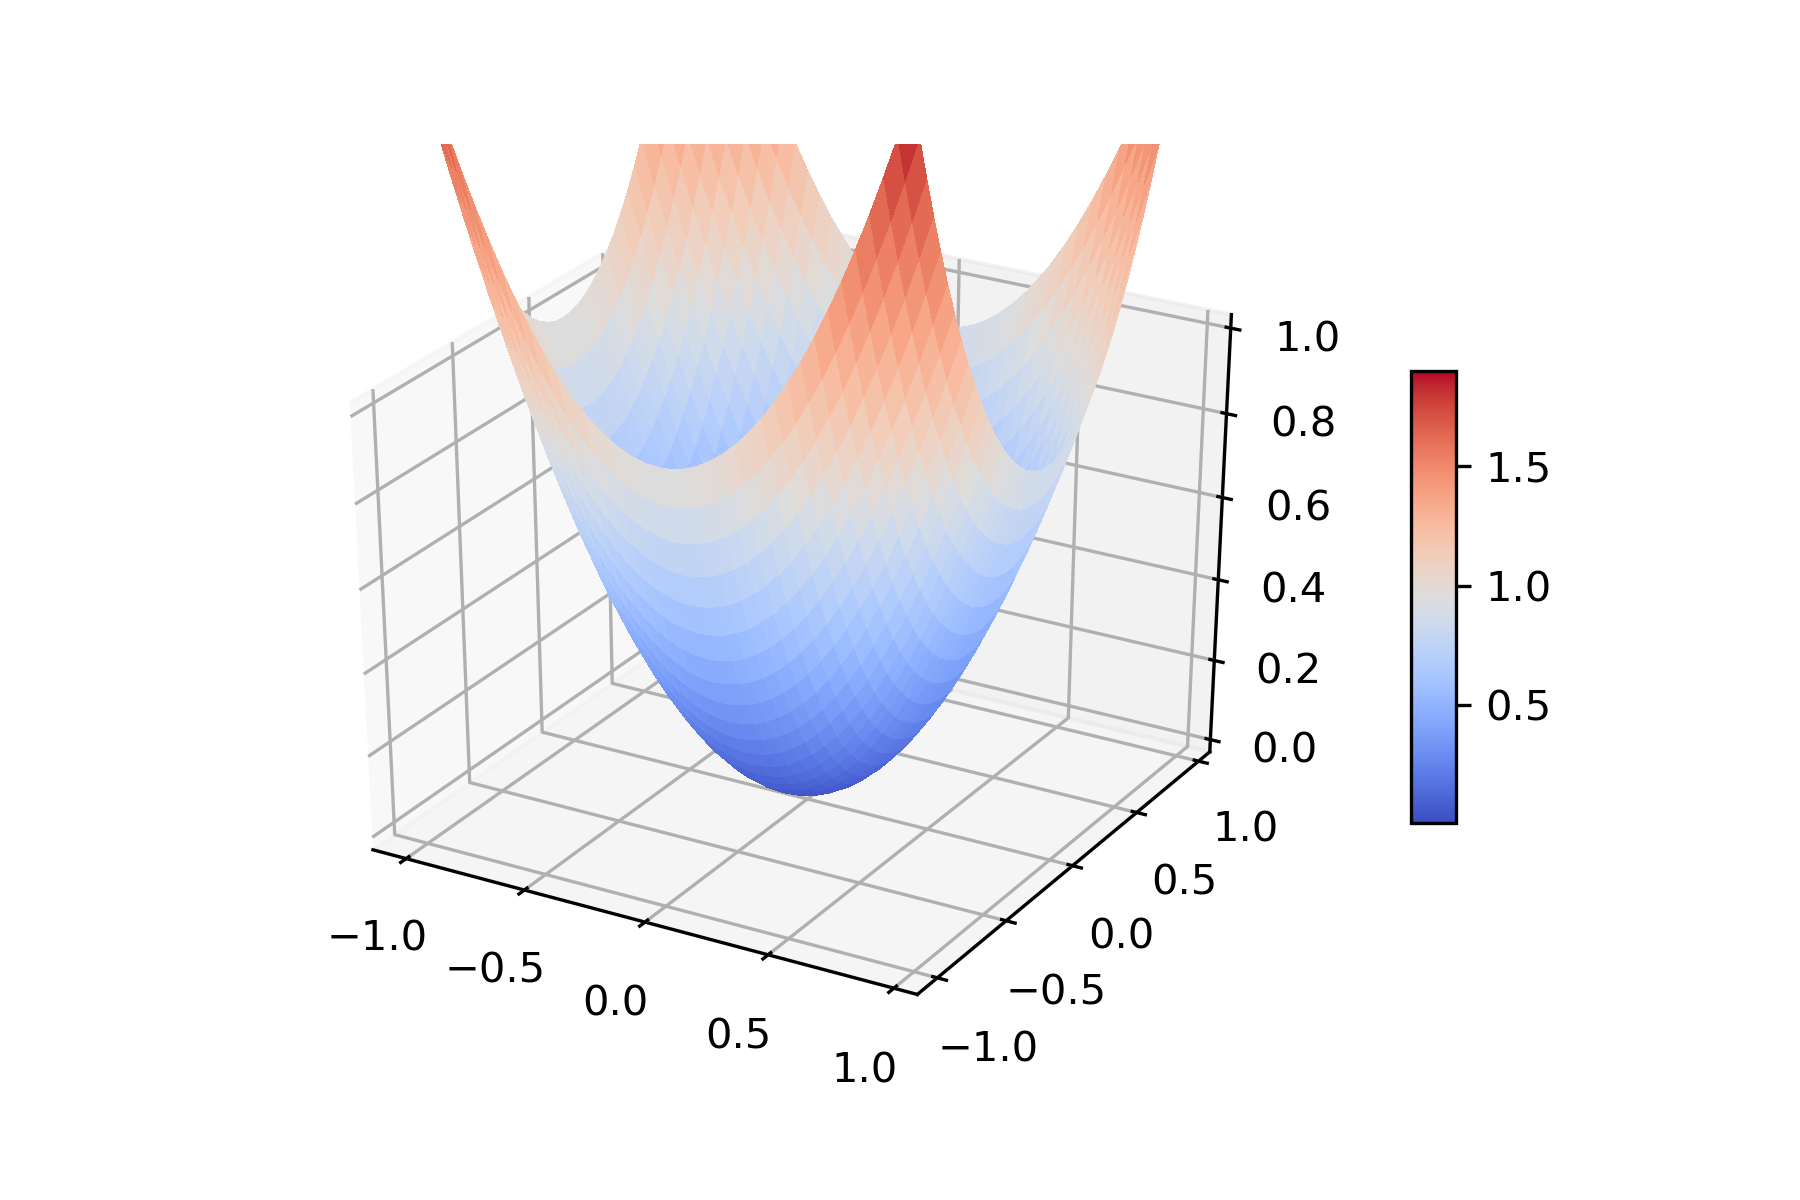
\includegraphics[scale = 0.5]{Figures/graph_positive.png}

\item Отрицательно определенная форма $z = - x^2 - y^2$.
Начало координат -- точка максимума.

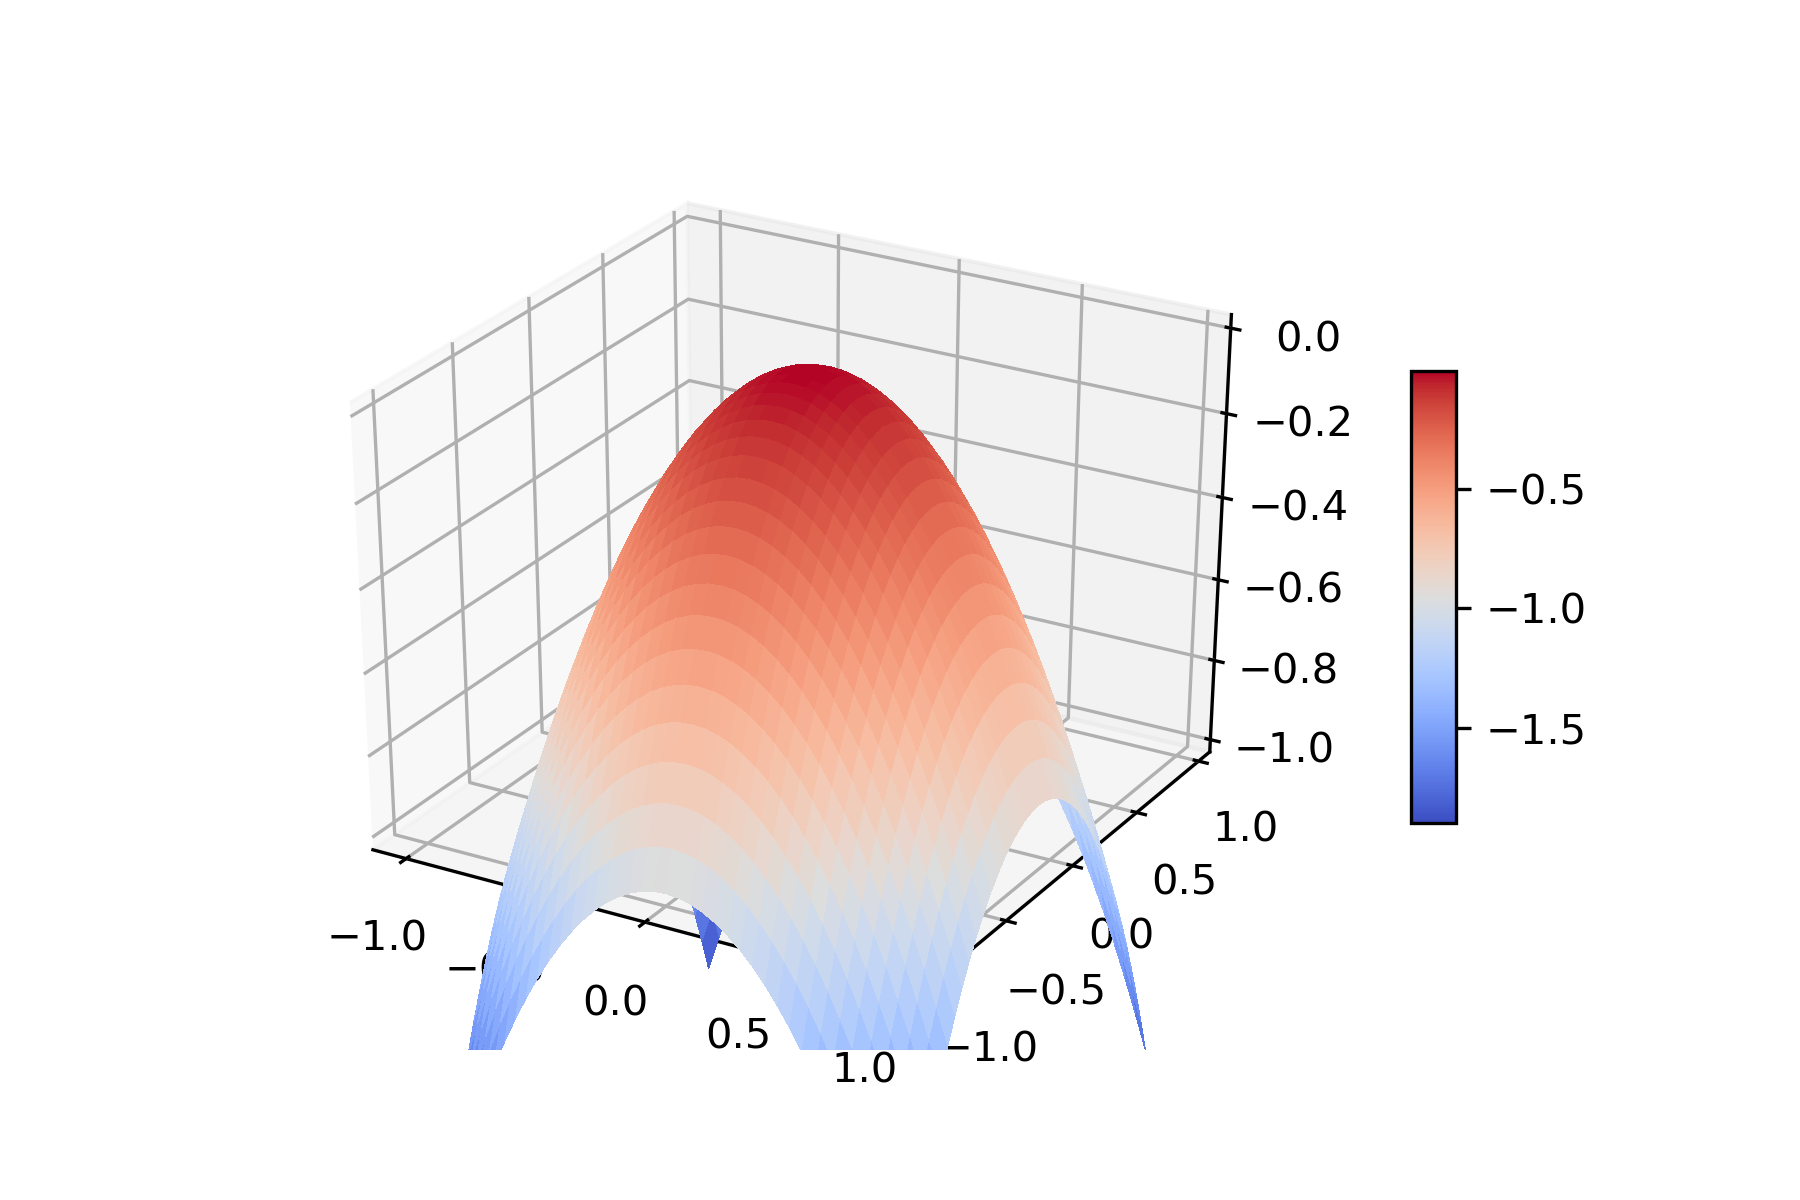
\includegraphics[scale = 0.5]{Figures/graph_negative.png}

\item Неотрицательно определенная форма $z = x^2$.
Минимум достигается на прямой $ x = 0$.

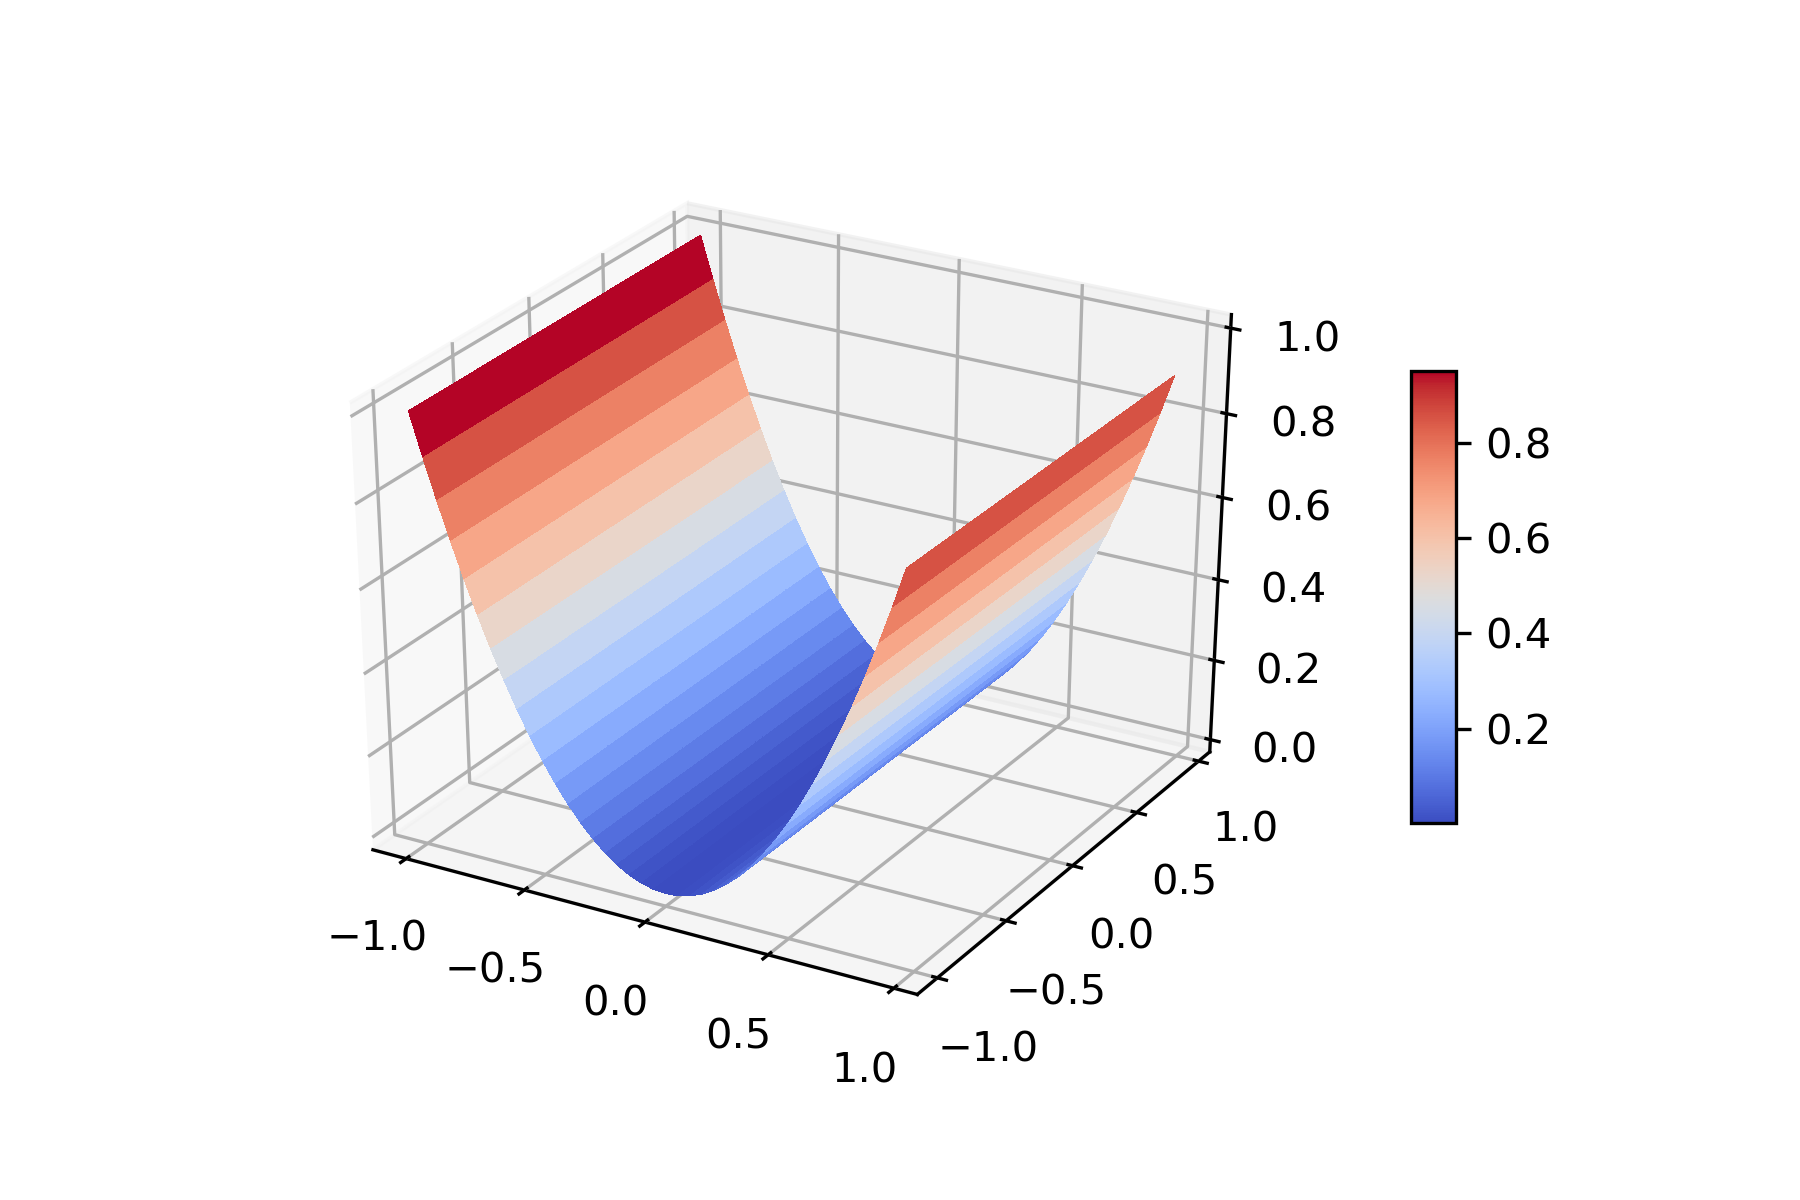
\includegraphics[scale = 0.5]{Figures/graph_non_negative.png}

\item Неположительно определенная форма $z = - x^2$.
Максимум достигается на прямой $x = 0$.

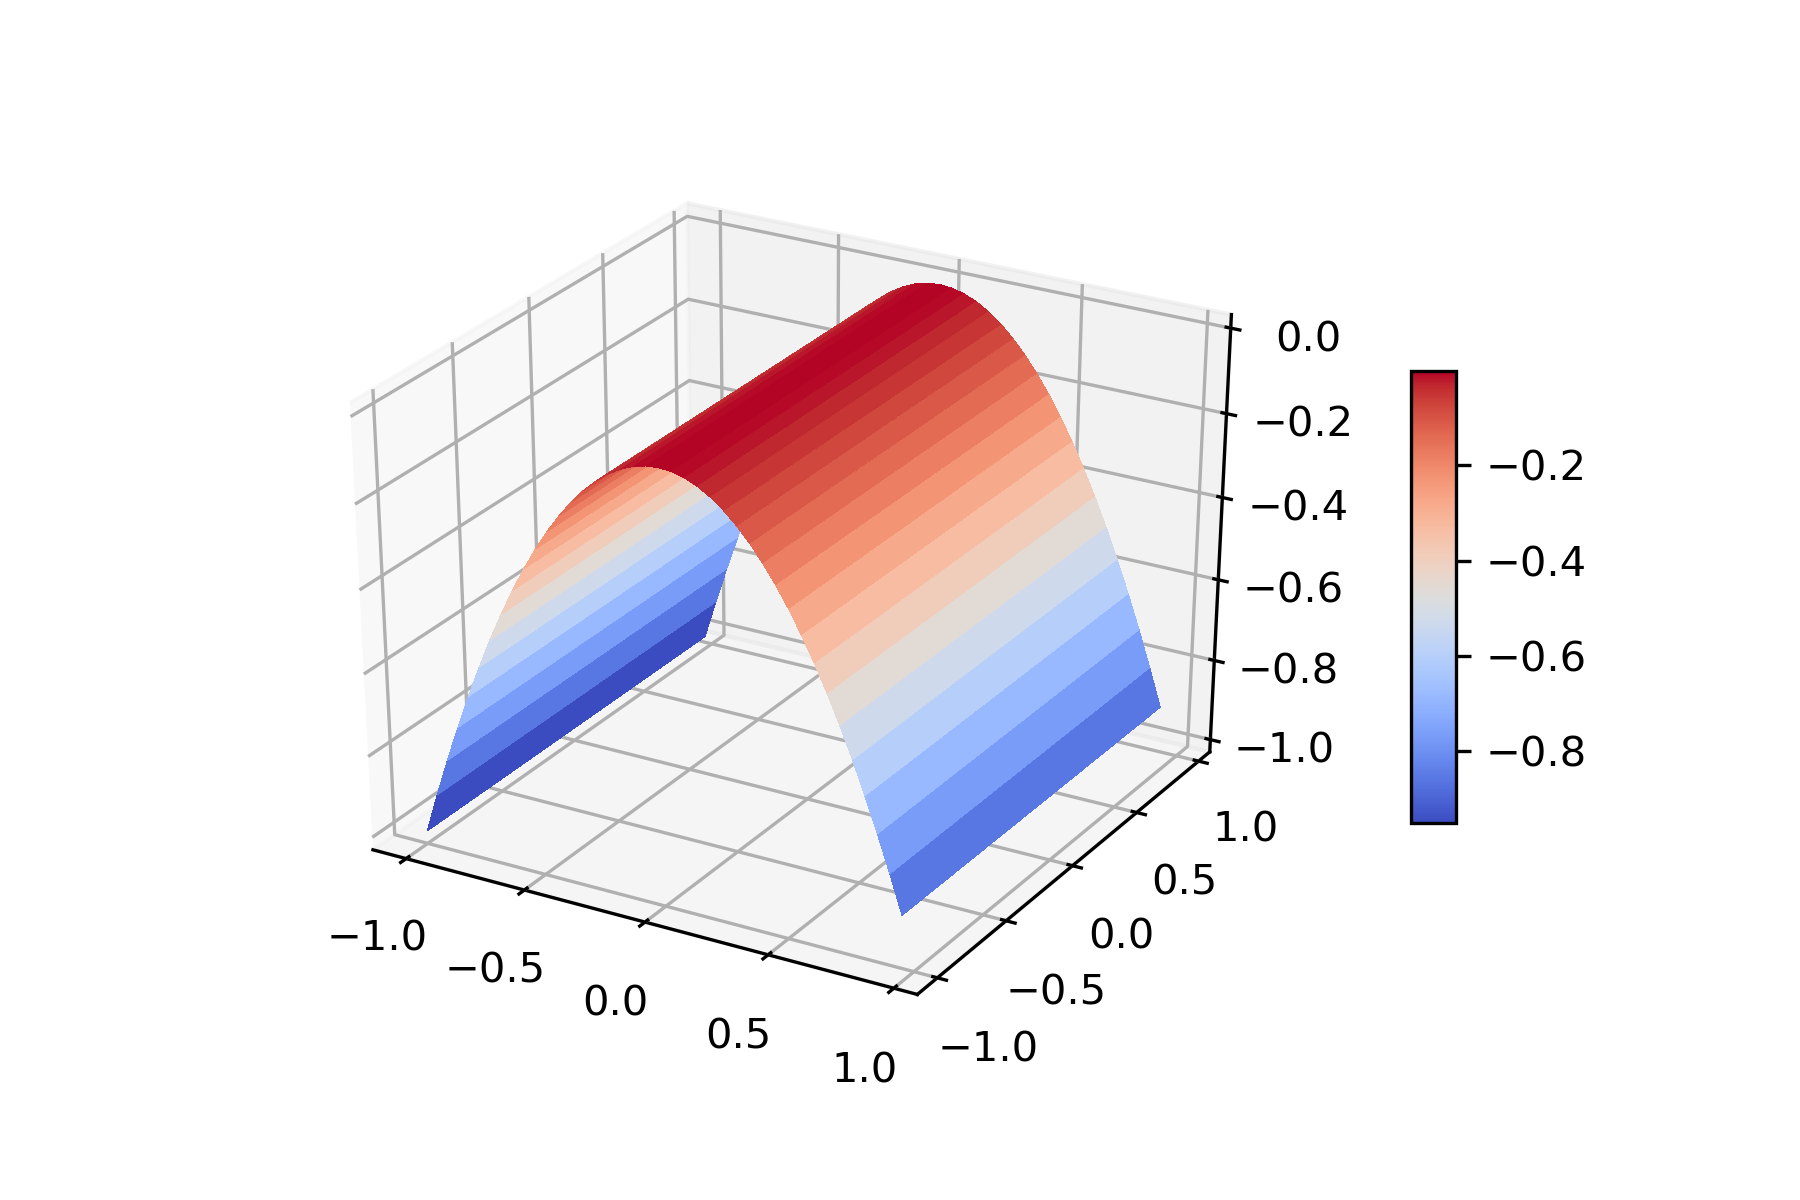
\includegraphics[scale = 0.5]{Figures/graph_non_positive.png}

\item Неопределенная форма $z = x^2 - y^2$.
Начало координат -- седловая точка.

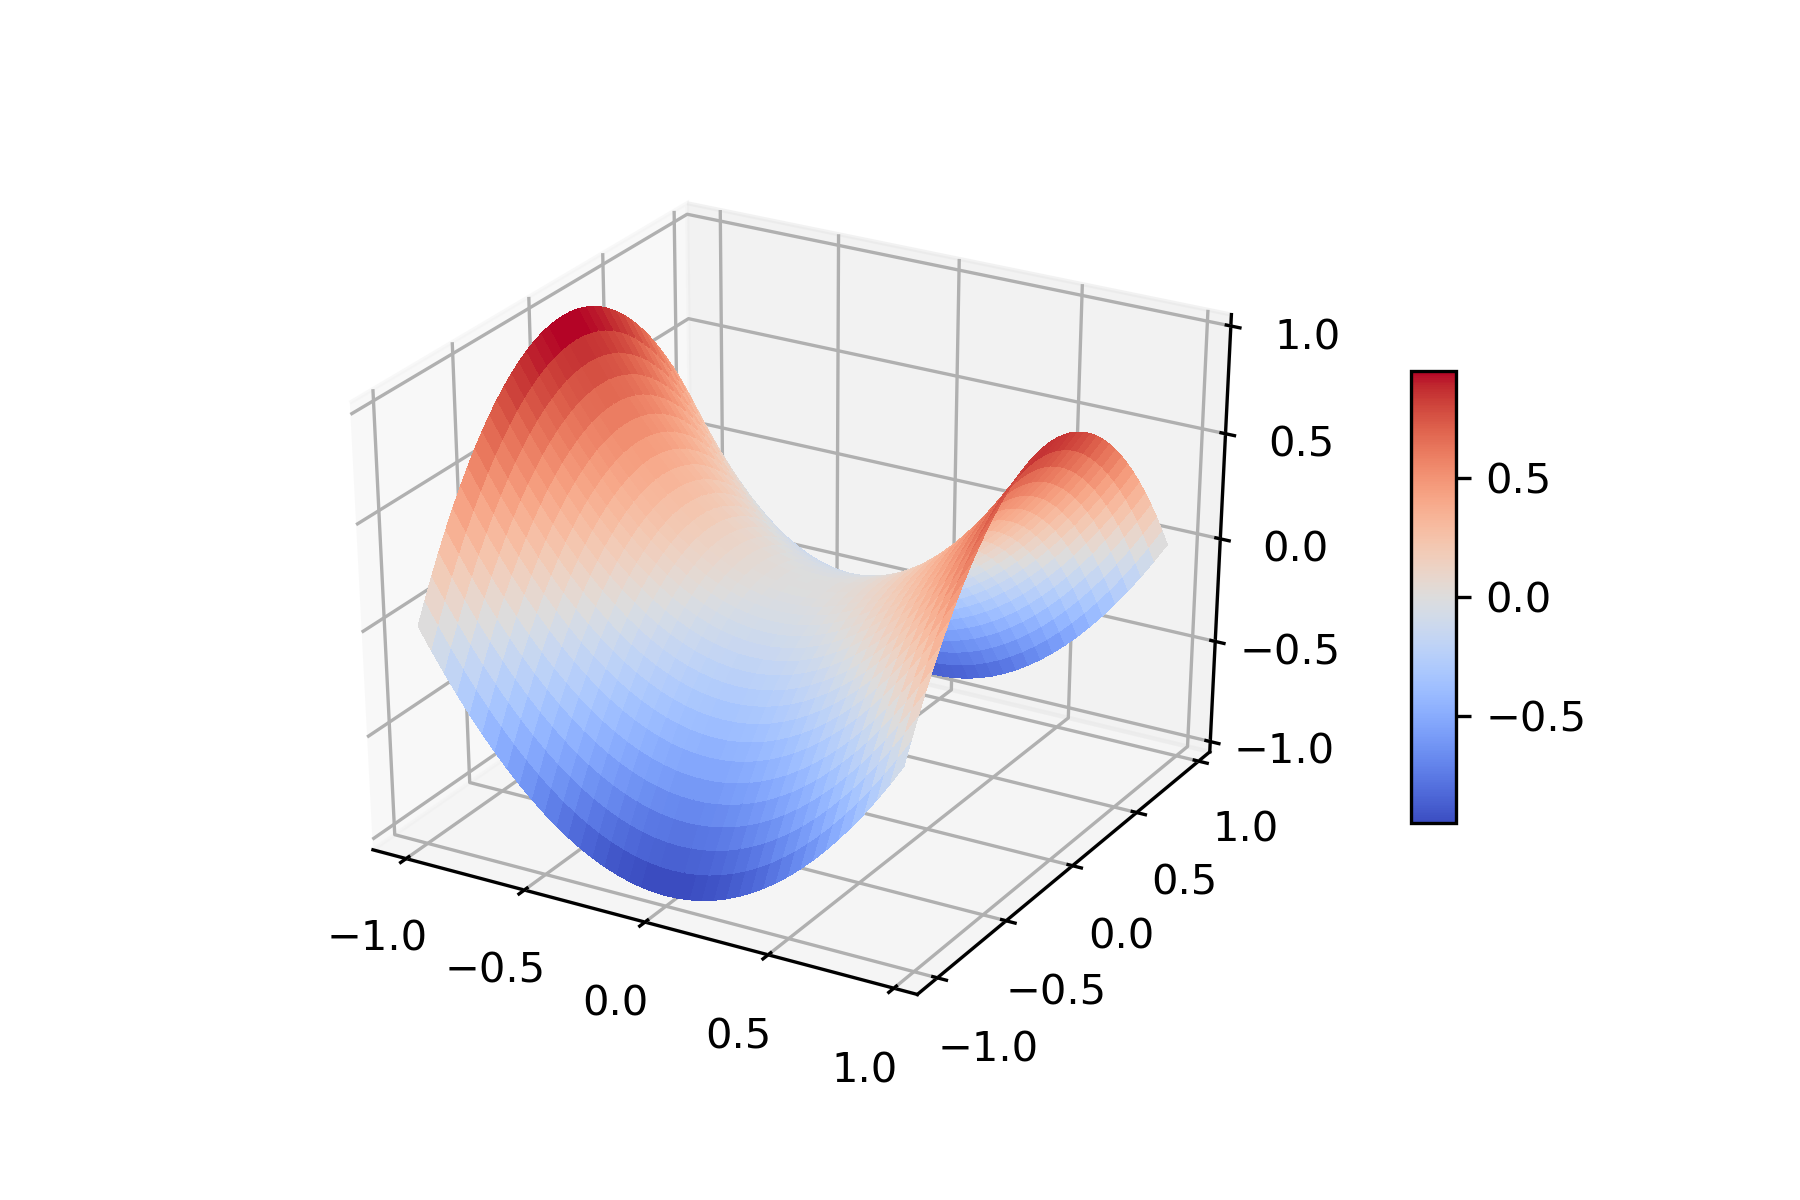
\includegraphics[scale = 0.5]{Figures/graph_saddle.png}
\end{enumerate}


\subsection{Анализ поверхности}

Квадратичные формы применяются для анализа поверхности графика функции от многих переменных.
Давайте я вкратце обрисую как.
Пусть $f\in C^2(\mathbb R^n)$ -- функция $n$ переменных, дифференцируемая дважды и вторые производные все непрерывны.
Тогда для любой точки $a\in \mathbb R^n$ выполнено разложение Тейлора
\[
f(z) = f(a) + \sum_{i=1}^n \frac{\partial f}{\partial x_i}(a)(z_i-a_i) + \sum_{ij=1}^n\frac{\partial^2 f}{\partial x_i\partial x_j}(a)(z_i-a_i)(z_j-a_j) + o(|z - a|^2)
\]
Здесь $o(|z-a|^2) = |z-a|^2 o(1)$, где $o(1)\to 0$ когда $z \to a$.
Геометрический смысл слагаемых следующий
\begin{enumerate}
\item Первое слагаемое $f(a)$ -- значение функции в точке.
Тут я никого этим не удивил.
Это лучшее приближение константой для нашей функции в точке $a$.

\item Второе слагаемое
\[
\sum_{i=1}^n \frac{\partial f}{\partial x_i}(a)(z_i-a_i)
\]
задает касательную плоскость в точке $a$ к графику функции $y = f(z)$.
То есть это линейное приближение для графика функции.
Эта плоскость горизонтальна тогда и только тогда, когда $ \frac{\partial f}{\partial x_i}(a) = 0$ для всех $1\leqslant i\leqslant n$.

\item Третье слагаемое 
\[
\sum_{ij=1}^n\frac{\partial^2 f}{\partial x_i\partial x_j}(a)(z_i-a_i)(z_j-a_j)
\]
является квадратичным приближением для графика функции.
Матрица с коэффициентами $\frac{\partial^2 f}{\partial x_i\partial x_j}(a)$ задает квадратичную форму называемую гессианом.
Если касательная плоскость горизонтальна, то сигнатура этой квадратичной формы определяет поведение графика в окрестности точки.
\begin{itemize}
\item Если форма положительно определена, то это точка локального минимума.

\item Если форма отрицательно определена, то это точка локального максимума.

\item Если форма не вырождена и неопределена, то это седловая точка
\end{itemize}
\end{enumerate}


\newpage
\section{Евклидовы пространства}

\subsection{Определение и примеры}

\begin{definition}
Евклидово пространство -- это пара $V$ и $({-},{-})$, где 
\begin{itemize}
\item $V$ -- векторное пространство над полем $\mathbb R$.

\item $({-},{-})\colon V\times V\to \mathbb R$ -- билинейная форма
\end{itemize}
При этом выполнены следующие аксиомы:
\begin{enumerate}
\item Форма $({-},{-})$ симметрическая.

\item Форма $({-},{-})$ положительно определена.
\end{enumerate}
Такая билинейная форма называется скалярным произведением.
\end{definition}

Очень часто, для краткости, когда задано евклидово пространство $V, ({-},{-})$, говорят, что $V$ является евклидовым пространством, подразумевая, что на нем есть скалярное произведение.

\paragraph{Примеры}

\begin{enumerate}
\item Пространство $\mathbb R^n$ со стандартным скалярным произведением $(x,y) = x^t y$.
Тогда $Q(x) = x^t x = \sum_{i=1}^n x_i^2 > 0$ при $x\neq 0$.

\item Пространство $\Matrix{n}$ со скалярным произведением $(A, B) = \tr(A^t B)$.
Тогда $Q(A) = \tr(A^t A) = \sum_{i,j=1}^n a_{ij}^2 > 0$ при $A\neq 0$.

\item Пусть $C[0,1]$ -- пространство непрерывных функций на отрезке $[0,1]$ сл скалярным произведением $(f,g) = \int_0^1 f(x) g(x)\,dx$.
Тогда $Q(f) = \int_0^1 f^2(x)\,dx > 0$ при $f \neq 0$.%
\footnote{В силу непрерывности, если $f(x)\neq 0$, то в какой-то окрестности $(x-\delta, x+\delta)$ точки $x$ имеем $|f(y)| > |f(x)| - \varepsilon$.}
\end{enumerate}

Важный вопрос: а как задавать скалярные произведения на некотором пространстве $V$?
Если в $V$ выбрать базис, то оно превратится в $\mathbb R^n$.
Тогда скалярное произведение задается симметричной матрицей $B$ с положительной сигнатурой.
Самый неудобный момент здесь заключается в том, что вообще говоря, глядя на матрицу $B$ не очевидно является ли она положительно определенной или нет.
Для этого надо пользоваться критерием Сильвестра (утверждение~\ref{claim::SilvCrit}).
Оказывается есть способ лучше, его мы обсудим далее.


\subsection{Ортогональные и ортонормированные базисы}

\begin{definition}
Пусть $V$ -- евклидово пространство.
Тогда
\begin{itemize}
\item Набор $v_1,\ldots,v_k\in V$ называется ортогональным, если $(v_i,v_j) = 0$ для всех $i\neq j$.


\item Набор $v_1,\ldots,v_k\in V$ называется ортонормированным, если он ортогонален и $(v_i,v_i) = 1$ для любого $i$.
\end{itemize}
Если $e_1,\ldots,e_n$ -- базис $V$, то он называется ортогональным или ортонормированным базисом, если набор $e_1,\ldots,e_n$ ортогонален или ортонормирован.
\end{definition}

\paragraph{Замечания}

\begin{itemize}
\item Базис является ортогональным тогда и только тогда, когда матрица скалярного произведения в нем диагональная.

\item Базис является ортонормированным тогда и только тогда, когда матрица скалярного произведения в нем единичная.

\item Утверждение~\ref{claim::SBilReal} говорит, что матрицу скалярного произведения всегда можно привести к единичной в некотором базисе.
То есть ортонормированные базисы существуют.

\item Процесс применяемый в методе Якоби (раздел~\ref{subsection::JacobyAlg}) превращает любой базис в ортогональный.%
\footnote{В евклидовых пространствах этот процесс называется процессом ортогонализации Грама-Шмидта.
Определение будет дальше.}
\end{itemize}


\begin{claim}
\label{claim::ScalarDef}
Пусть $V$ -- векторное пространство над $\mathbb R$.
Тогда для любого базиса $e_1,\ldots,e_n$ существует единственное скалярное произведение $({-},{-})$ на $V$ такое, что $e_1,\ldots,e_n$ является ортонормированным базисом.
\end{claim}
\begin{proof}
Зафиксируем базис $e_1,\ldots,e_n$.
Тогда задать билинейную форму -- это все равно, что задать матрицу $B\in \Matrix{n}$ (утверждение~\ref{claim::BilinearMatrices}).
Когда такая матрица $B$ задает скалярное произведение, в котором $e_1,\ldots,e_n$ -- ортонормированный базис?
Тогда и только тогда, когда $B = E$.
\end{proof}

По ортогональным и ортонормированным базисам удобно раскладывать произвольные векторы.

\begin{claim}
Пусть $V$ -- евклидово пространство, $e_1,\ldots,e_n$ -- базис и $v\in V$ -- произвольный вектор.
Тогда
\begin{enumerate}
\item Если $e_1,\ldots,e_n$ ортогональный, то 
\[
v = \frac{(v,e_1)}{(e_1,e_1)}e_1 + \ldots + \frac{(v,e_n)}{(e_n,e_n)} e_n
\]

\item Если $e_1,\ldots,e_n$ ортонормированный, то
\[
v = (v,e_1)e_1+\ldots+(v,e_n)e_n
\]
\end{enumerate}
\end{claim}
\begin{proof}
Вторая формула есть элементарное следствие первой, так как $(e_i,e_i) = 1$ для ортонормированного базиса.
Потому достаточно доказать первую формулу.
Пусть $v = \alpha_1e_1+\ldots+\alpha_n e_n$.
Умножим скалярно левую и правую часть на вектор $e_k$, тогда получим $(v, e_k) = \sum_{i=1}^n \alpha_i(e_i, e_k) = \alpha_k (e_k,e_k)$.
Значит, $\alpha_k = \frac{(v,e_k)}{(e_k,e_k)}$, что и требовалось.
\end{proof}


\begin{claim}
Пусть $A\in \Matrix{n}$.
Тогда следующие условия равносильны
\begin{enumerate}
\item $A^t A = E$.

\item $AA^t = E$.

\item $A^t = A^{-1}$.
\end{enumerate}
\end{claim}
\begin{proof}
Это следует из существования и единственности обратного при наличии левого или правого обратного (утверждение~\ref{claim::InvertibleDiscription}).
\end{proof}

\begin{definition}
Матрица $A\in \Matrix{n}$ называется ортогональной, если выполнено одно из эквивалентных свойств из предыдущего утверждения, например, $A^t A = E$.
\end{definition}

\paragraph{Замечание}

Рассмотрим в $\mathbb R^n$ стандартное скалярное произведение.
Если $A\in\Matrix{n}$, то условие $A^t A = E$ означает, что столбцы матрицы $A$ образуют ортонормированный базис.
Условие $A A^t = E$ означает, что строки матрицы $A$ образуют ортонормированный базис.
Важно понимать, что эти условия эквивалентны.
А именно, если вы возьмете ортонормированный базис в $\mathbb R^n$ и поставите эти векторы в столбцы матрицы $A$, то строки этой матрицы автоматически образуют некий другой ортонормированный базис в $\mathbb R^n$.

\begin{claim}
\label{claim::OrthoBasisDiscrEucl}
Пусть $V$ -- евклидово пространство.
Тогда
\begin{enumerate}
\item Если $e_1,\ldots,e_n$ и $f_1,\ldots,f_n$ -- два ортонормированных базиса, то матрица перехода между ними будет ортогональна.

\item Если $e_1,\ldots,e_n$ -- ортонормированный базис и $C\in \Matrix{n}$ -- ортогональная матрица, то базис $(e_1,\ldots,e_n)C$ будет ортонормированным.
\end{enumerate}
\end{claim}
\begin{proof}
(1) Пусть $(f_1,\ldots,f_n) = (e_1,\ldots,e_n)C$, где $C\in \Matrix{n}$.
Так оба базиса ортонормированные, то матрица скалярного произведения в каждом из этих базисов единичная.
По правилу изменения матрицы билинейной формы при смене базиса получаем $E = C^t E C$.
Значит $C$ ортогональная.

(2) Пусть $(f_1,\ldots,f_n) = (e_1,\ldots,e_n)C$.
В базисе $e_1,\ldots,e_n$ матрица билинейной формы $E$, так как он ортонормированный.
Матрица в базисе $f_1,\ldots,f_n$ будет $C^t E C$.
Так как $C$ ортогональная, то это будет $E$, то есть $f_1,\ldots,f_n$ -- ортонормированный базис.
\end{proof}

Таким образом за переход между ортонормированными базисами отвечают только ортогональные матрицы.

\subsection{Классификация Евклидовых пространств}

Если у нас есть два векторных пространства $V$ и $U$, то они изоморфны (то есть по сути одно и то же векторное пространство, но заданное по-разному) тогда и только тогда, когда у них одинаковые размерности (утверждение~\ref{claim::VectorClassific}).
Теперь мы хотим решить ту же самую задачу для евклидовых пространств -- понять, когда они будут одинаковыми.
Для начала надо объяснить, что значит изоморфизм евклидовых пространств.

\begin{definition}
Пусть $V$ и $U$ -- два евклидовых пространства.
Линейное отображение $\phi\colon V\to U$ называется изоморфизмом евклидовых пространств, если
\begin{enumerate}
\item $\phi$ -- изоморфизм векторных пространств.

\item Для любых $v,u\in V$ выполнено $(v, u) = (\phi(v), \phi(u))$.%
\footnote{Здесь слева скалярное произведение в пространстве $V$, а с права в пространстве $U$.}
\end{enumerate}
При наличии изоморфизма между евклидовыми пространствами $V$ и $U$ они называются изоморфными.
\end{definition}

Второе условие в определении можно выразить коммутативностью следующей диаграммы
\[
\xymatrix@R=6pt@C=40pt{
	{V\times V}\ar[dd]^{\phi\times \phi}\ar[rd]&{}&{(v,u)}\ar@{|->}[dd]\ar@{|->}[rd]&{}\\
	{}&{\mathbb R}&{}&{(v,u) = (\phi(v),\phi(u))}\\
	{U\times U}\ar[ru]&{}&{(\phi(v),\phi(u))}\ar@{|->}[ru]&{}
}
\]
Смысл определения в том, что при изоморфизме не только вектора и операции над ними переходят в соответствующие вектора и операции, но и скалярное произведение на первом пространстве превращается в скалярное произведение на втором после применения измоморфизма.
Значит при таком изоморфизме вся структура евклидова пространства сохраняется, а значит мы считаем, что такие пространства одинаковые, как евклидовы пространства.
Более того, все свойства таких пространств (если они выражены в терминах евклидова пространства) одинаковые и одно можно безболезненно менять на другое, если это удобно.


\begin{claim}
\label{claim::EuclideanIsom}
Два евклидовых пространства $V$ и $U$ изоморфны тогда и только тогда, когда $\dim V = \dim U$.
\end{claim}
\begin{proof}
Ясно, что у изоморфных пространств одинаковая размерность.
Потому надо показать, что из условия $\dim V = \dim U$ найдется изоморфизм, согласованный со скалярным произведением.
Давайте выберем ортонормированный базис $e_1,\ldots,e_n$ в $V$ и ортонормированный базис $f_1,\ldots,f_n$ в $U$.
Тогда построим линейное отображение $\phi\colon V\to U$ отправляющее $e_i\mapsto f_i$ (такое найдется единственное по утверждению~\ref{claim::LinMapExist}).
Если векторы $v,u\in V$ имеют координаты $x,y\in \mathbb R^n$ в базисе $e_1,\ldots,e_n$, то векторы $\phi(v),\phi(u)\in U$ имеют те же самые координаты $x,y$ в базисе $f_1,\ldots,f_n$.
Тогда $(v,u) = x^ty$ и $(\phi(v),\phi(u)) = x^ty$.
\end{proof}

\paragraph{Замечания}

\begin{itemize}
\item Таким образом добавление скалярного произведения к пространству не увеличивает количество не изоморфных векторных пространств.

\item Пространство $\mathbb R^2$ со стандартным скалярным произведением является <<школьной плоскостью>>, которую мы все долго и упорно изучали в курсе геометрии школьной программы.
А пространство $\mathbb R^3$ со стандартным произведением является <<школьным пространством>>.

\item Самым важным с идейной точки зрения является следующее наблюдение, которое вытекает из предыдущего утверждения.
Пусть мы хотим доказать что-то про два вектора $v,u\in V$ в каком-то евклидовом пространстве.
Тогда они обязательно содержатся в каком-то двумерном подпространстве $U\subseteq V$.
Само $U$ тоже является евклидовым вместе с ограничением скалярного произведения с $V$.
Но у нас есть школьная плоскость, которая тоже является двумерным евклидовым пространством.
А значит, это то же самое пространство, что и $U$.
То есть нам достаточно доказать факт для произвольных двух векторов на школьной плоскости.
Получается, что автоматически можно пользоваться результатами школьной геометрии.
Аналогичная идея работает с тремя векторами и сведением задачи к школьной стереометрии.

\item Несмотря на то, что можно пользоваться школьной геометрией, бывает полезно понять, как именно доказывать те или иные утверждения пользуясь формализмами линейной алгебры напрямую.
Потому я буду периодически демонстрировать какие-то вещи в лоб.
\end{itemize}


\subsection{Геометрия в Евклидовых пространствах}

\begin{definition}
Пусть $V$ -- евклидово пространство и $v\in V$ -- произвольный вектор.
Определим длину вектора $|v| = \sqrt{(v,v)}$.
\end{definition}

\paragraph{Замечания}

\begin{itemize}
\item Именно для того, чтобы определить длину произвольного вектора, нам нужна положительная определенность в определении скалярного произведения.

\item Обратите внимание, что $|v| = 0$ тогда и только тогда, когда $v = 0$.

\item Если выбрать ортонормированный базис, то $|x| = \sqrt{\sum_{i=1}^n x_i^2}$.
То есть это $|{-}|_2$ норма на $\mathbb R^n$.
На самом деле можно развивать теорию норм на произвольных векторных пространствах, как это делается в функциональном анализе.
\end{itemize}

\begin{claim}
[Неравенство Коши-Буняковского]
Пусть $V$ -- евклидово пространство, $v,u\in V$, тогда $|(v,u)|\leqslant |v| |u|$.
Кроме того, равенство достигается тогда и только тогда, когда $u$ и $v$ лежат на одной прямой.
\end{claim}
\begin{proof}
Так как у нас всего два вектора, можно считать, что $V$ двумерно.
Выберем первый базисный вектор $e_1$ вдоль $v$ (если $v$ нулевой, то выбираем любой), а второй -- любой ортогональный к $e_2$ и длины $1$.
Тогда
\[
v = 
\begin{pmatrix}
{a}\\{0}
\end{pmatrix}
\quad\text{и}\quad
u = 
\begin{pmatrix}
{b}\\{c}
\end{pmatrix}
\]
Тогда $|(v, u)| = |ab|$, а $|v||u| = |a|\sqrt{b^2 + c^2}$.
Доказываемое неравенство превращается в $|ab|\leqslant |a|\sqrt{b^2 + c^2}$, что очевидно.

Давайте проанализируем, когда в нем достигается равенство.
Во-первых, если $a = 0$.
В этом случае $v$ и $u$ лежат на одной прямой.
Если $a \neq 0$, то мы получаем условие $|b| = \sqrt{b^2 + c^2}$, что равносильно тому, что $c = 0$.
В этом случае векторы тоже лежат на одной прямой.
Обратно, если векторы лежат на одной прямой, то $v = \lambda e$ и $u = \mu e$ для некоторого ненулевого вектора $e\in V$.
Тогда $(v,u) = \lambda\mu (e,e)$, а с другой стороны $|v||u| = |\lambda e||\mu e| = |\lambda \mu| |e|^2 = |\lambda \mu|(e,e)$.
\end{proof}

\paragraph{Замечание} 

Хочу обратить внимание на то, что по сути доказательство можно было закончить на первой строчке, где я ссылаюсь  на школьную геометрию.
Вся остальная часть всего лишь доказывала факт из школьной геометрии.
Это было сделано для полноты изложения.
К тому же я продемонстрировал метод последовательного выбора удобных базисных векторов, который часто применяется при решении задач аналитической геометрии.
Подобный метод позволяет упростить разбор общего случая в координатах за счет наличия большого количества нулей в векторах.
В нашем случае ноль был всего один, но это сильно сократило вычисления.

Из неравенства Коши-Буняковского следует, что для любых двух ненулевых векторов $v,u\in V$ верно $-1\leqslant \frac{(v,u)}{|v| |u|}\leqslant 1$.
А значит найдется единственное число $\alpha\in [0,\pi]$ такое, что $\cos \alpha = \frac{(v,u)}{|v| |u|}$.

\begin{definition}
Пусть $V$ -- евклидово пространство и $v,u\in V$ -- два вектора.
Тогда число $\alpha$ такое, что $\cos \alpha = \frac{(v,u)}{|v| |u|}$, называется углом между векторами $v$ и $u$.
Будем этот угол обозначать через $\angle(v, u)$.
\end{definition}

\paragraph{Замечание}

Так как два вектора $v$ и $u$ всегда лежат внутри <<школьной плоскости>>, то определение угла превращается в то самое определение угла, которое дается в школьном курсе геометрии.
Потому от этого угла надо ожидать ровно то же самое поведение, к которому мы привыкли в курсе школьной геометрии.
Просто потому, что это тот же самый угол.


\begin{claim}
[Теорема Пифагора]
\label{claim::Pythagoras}
Пусть $V$ -- евклидово пространство и $v,u\in V$ -- два ортогональных вектора, тогда $|v + u|^2 = |v|^2 + |u|^2$.
\end{claim}
\begin{proof}
Формальное доказательство в этом случае является наиболее простым:
\[
|v+u|^2 = (v+u, v+u) = (v,v) + (v,u)+(u,v) +(u,u) = (v,v) + (u,u) = |v|^2 + |u|^2
\]
Здесь $(v,u)=(u,v) = 0$ из ортогональности $u$ и $v$.
\end{proof}

Процесс, применяемый к базисным векторам в методе Якоби (раздел~\ref{subsection::JacobyAlg}), в случае евклидова пространства называется ортогонализацией Грама-Шмидта.
Единственное отличие -- ортогонализация Грама-Шмидта применяется не только к линейно независимым векторам, а к произвольным системам векторов.

\subsubsection*{Ортогонализация методом Грама-Шмидта}

\paragraph{Дано}

Евклидово пространство $V$, система векторов $\{v_1,\ldots,v_k\}\subseteq V$.%
\footnote{Обратите внимание, что $V$ не обязательно задано как пространство столбцов $\Vector{n}$.
Это может быть и пространство многочленов определенной степени или пространство тригонометрических функций, или вообще что угодно.
Даже если $V$ задано как $\Vector{n}$, то скалярное произведение не обязательно стандартное, т.е. скалярное произведение может быть задано любой положительной симметрической матрицей.}

\paragraph{Задача}

Найти систему ортогональных векторов $\{u_1,\ldots,u_r\}\subseteq V$ такую, что $\langle v_1,\ldots,v_k\rangle = \langle u_1,\ldots,u_r\rangle$.

\paragraph{Алгоритм}

\begin{enumerate}
\item В качестве первого вектора $u_1$ берем первый ненулевой вектор из $v_i$.
Если таких нет, то ответ -- пустое множество.

\item Пусть мы нашли вектора $u_1,\ldots,u_s$ и пусть $v_d$ -- первый еще не просмотренный вектор среди $v_i$.
Посчитать вектор 
\[
u' = v_d - \frac{(v_d, u_1)}{(u_1,u_1)} u_1 - \ldots - \frac{(v_d, u_s)}{(u_s, u_s)}u_s
\]

\item Если $u' \neq 0$ положим $u_{s+1} = u'$, иначе пропустим $v_d$.
Теперь перейдем к предыдущему шагу с вектором $v_{d+1}$ вместо $v_d$.
\end{enumerate}

% Надо переместить вперед, ближе к объемам
\subsection{Матрица Грама}
\label{subsection::Gram}

Давайте поговорим о еще одном объекте, который возникает в связи с конечной системой векторов в Евклидовом пространстве.
Таким объектом является матрица Грама.
Она в частности используется для определения объемов.

\begin{definition}
Пусть $V$ -- евклидово пространство и $v_1,\ldots,v_k\in V$ -- произвольный набор векторов ($k$ НЕ обязательно равно размерности пространства).
Тогда матрица
\[
G(v_1,\ldots,v_k) =
\begin{pmatrix}
{(v_1,v_1)}&{\ldots}&{(v_1,v_k)}\\
{\vdots}&{\ddots}&{\vdots}\\
{(v_k,v_1)}&{\ldots}&{(v_k,v_k)}\\
\end{pmatrix}
\in\Matrix{k}
\]
называется матрицей Грама системы векторов $v_1,\ldots,v_k$.%
\footnote{Обратите внимание, тут важен порядок векторов.
То есть формально матрица Грама зависит от набора $(v_1,\ldots,v_k)\in V^k$.}
\end{definition}

Если $e_1,\ldots,e_n$ -- некоторый базис пространства $V$, то $B = G(e_1,\ldots,e_n)$ -- матрица скалярного произведения заданная в базисе $e_1,\ldots,e_n$.
Таким образом матрица Грама -- это некоторое обобщение матрицы билинейной формы.

Теперь вспомним, что у любой билинейной формы есть операторная запись.
Давайте введем следующее обозначение: для произвольных векторов $w, u\in V$ положим $w\cdot u = (w, u)$.
Тогда для набора $v = (v_1,\ldots,v_k)$ выполнено
\[
G(v_1,\ldots,v_k) = 
\begin{pmatrix}
{v_1}\\{\vdots}\\{v_k}
\end{pmatrix}
\cdot
\begin{pmatrix}
{v_1}&{\ldots}&{v_k}
\end{pmatrix}
=
v^t \cdot v
\]

Пусть теперь $C\in \MatrixDim{k}{r}$ -- некоторая матрица.
Тогда из набора $(v_1,\ldots,v_k)$ можно построить новый набор $(u_1,\ldots,u_r) = (v_1,\ldots,v_k)C$ или кратко $u = vC$.
Тогда 
\[
G(u) = G(vC) = (vC)^t \cdot vC = C^t v^t \cdot v C = C^t G(v) C
\]
То есть $G((v_1,\ldots,v_k)C) = C^t G(v_1,\ldots,v_k)C$.


\begin{claim}
\label{claim::GramMatrixFull}
Пусть $v_1,\ldots,v_k\in V$ -- произвольный набор векторов в евклидовом пространстве.
Тогда
\begin{enumerate}
\item Пусть $\alpha_1,\ldots,\alpha_k \in \mathbb R$, введем обозначение $\alpha = (\alpha_1,\ldots,\alpha_k)^t$.
Тогда следующие условия эквивалентны:
\begin{enumerate}
\item $\alpha_1 v_1 + \ldots + \alpha_k v_k = 0$.

\item $G(v_1,\ldots,v_k)\alpha= 0$.

\item $\alpha^tG(v_1,\ldots,v_k)\alpha= 0$.
\end{enumerate}
\item $\rk G(v_1,\ldots,v_k) = \dim \langle v_1,\ldots,v_k\rangle$.

\item  $\det G(v_1,\ldots,v_k)\geqslant 0$.
При этом равенство достигается тогда и только тогда, когда векторы линейно зависимы.

\item Если $C\in\Matrix{k}$ является матрицей элементарного преобразования I или II типа, то 
\[
\det G(v_1,\ldots,v_k) = \det G((v_1,\ldots,v_k)C)
\]
\end{enumerate}
\end{claim}
\begin{proof}
1) Пусть $v = (v_1,\ldots,v_k)$.
Тогда условие $v\alpha = 0$ влечет, что $v^t \cdot v\alpha = 0$.
Но это означает, что $G(v_1,\ldots,v_k) \alpha = 0$.
Домножая слева на $\alpha^t$ получаем, что $\alpha^t G(v_1,\ldots,v_k) \alpha = 0$.
Осталось показать из последнего в первое.
Для этого заметим, что $0 = \alpha^t G(v_1,\ldots,v_k) \alpha = \alpha^t v^t \cdot v\alpha = (v\alpha, v\alpha)$.
А значит $v\alpha = 0$.

2) Пункт~(1) эквивалентность (a) и (b) означает, что векторы $v_1,\ldots,v_k$ обладают теми же линейными зависимостями, что и столбцы матрицы $G(v_1,\ldots,v_k)$.
В частности столбцовый ранг $G(v_1,\ldots,v_k)$ равен рангу системы векторов $(v_1,\ldots,v_k)$.
А последняя совпадает с размерностью линейной оболочки $\langle v_1,\ldots,v_k\rangle$.

3) Давайте на пространстве $\mathbb R^k$ рассмотрим билинейную форму $\beta(x,y) = x^t G(v_1,\ldots,v_k)y$.
Давайте покажем, что она не отрицательно определена.
Тогда, ее определитель должен быть не отрицательным.
Действительно, тогда в каком-то базисе ее матрица диагональна с $1$ и $0$ на диагонали, а значит в этом базисе определитель будет неотрицательным.
Но определитель билинейной формы не меняет знак при замене базиса (раздел~\ref{subsection::BilChar}).
Теперь остается лишь проверить, что $\beta(x,x)\geqslant 0$ для любого $x\in \mathbb R^k$.
Действительно
\[
x^t G(v_1,\ldots,v_k) x = x^t v^t\cdot v x = (vx, vx) \geqslant 0
\]
Последнее неравенство выполнено для любого вектора $vx\in V$ по определению скалярного произведения.

4) Если $C$ -- матрица элементарного преобразования, то $G((v_1,\ldots,v_k)C) = C^t G(v_1,\ldots,v_k)C$.
А значит $\det(G((v_1,\ldots,v_k)C)) = \det(G(v_1,\ldots,v_k))\det C^2$.
Но для элементарных преобразований I и II типов $\det C = \pm 1$.
\end{proof}

Заметим, что из третьего пункта следует вот какое наблюдение.
Если $v_1,\ldots, v_k$ -- линейно независимый набор векторов, из которого процессом ортогонализации Грама-Шмидта мы получили набор $u_1,\ldots,u_k$, то $\det G(u_1,\ldots,u_k) = \det G(v_1,\ldots,v_k)$.


\end{document}
